\documentclass[11pt, twoside, openright]{book}

% DA CITARE FONTE: https://icons8.com/icons/set/light-o

% aggiungere in piccolo "a cura di jb"

%%% Font, caratteri speciali e lingua %%% 
\usepackage[T1]{fontenc}
\usepackage[utf8]{inputenc}
\usepackage[french]{babel}

%%% Per ringraziamenti a forma di cuore
\usepackage{shapepar}
\usepackage{lipsum} % For placeholder text

%%% simbolo mail
\usepackage{fontawesome}

%\raggedbottom %annulla riempimento della pagina in verticale con spazi aggiuntivi tra capoversi o ambienti

%%% Stile della pagina %%%
\pagestyle{headings} %Ved. p. 35
\usepackage{emptypage}
%%%%%%%%%%%%%%%%

\usepackage{graphicx}
\usepackage[paperheight=9in, paperwidth=6in]{geometry}
%\usepackage[a4paper]{geometry}
\usepackage{afterpage}
\usepackage[svgnames, dvipsnames]{xcolor}

\usepackage{pagecolor}
%\usepackage{gfsdidot}
\usepackage{charter}
\usepackage{qrcode}
\usepackage{etoolbox}
\renewenvironment{quote}{%
   \list{}{%
     \leftmargin0.1cm   % this is the adjusting screw
     \rightmargin\leftmargin
   }
   \item\relax
}
{\endlist}


\DeclareRobustCommand{\augiefamily}{%
  \fontfamily{augie}\fontseries{m}\fontshape{n}\selectfont}
\DeclareTextFontCommand{\textaugie}{\augiefamily}

\usepackage[object=vectorian]{pgfornament}

\usepackage{changepage}

\usepackage{titling}
\patchcmd{\titlepage}{\setcounter{page}\@ne}{}{\message {Successfully patched titlepage.}}{\message {Failed to patch titlepage.}}


\usepackage[skins]{tcolorbox}

%%%%%%%%%%%%%%%%%%%%%%%%%%
% Dedication's package
\usepackage{emerald}
\pdfmapfile{=emerald.map}
%%%%%%%%%%%%%%%%%%%%%%%%%%

\newtcbox{\whiteshadowbox}[1][]{%
  enhanced, 
  center upper,
  fontupper=\large\bfseries,
  drop fuzzy shadow southeast,
  boxrule=0pt,
  sharp corners,
  colframe=blue,
  colback=white!10,
  before={\begin{center}},
    after={\end{center}},
  #1%
}
%%%%%%%%%%%%%%%%%%%%%%%%%
\usepackage{tocloft}


%%% PACKAGES
\usepackage{dramatist}

\usepackage{titling}% Allows for multiple \titles within one document

\let\oldmaketitle\maketitle
\renewcommand{\maketitle}{%
\newpage
\phantomsection
  \addcontentsline{toc}{chapter}{\thetitle}
\oldmaketitle

\markboth{\MakeUppercase{\thetitle}}{\MakeUppercase{\thetitle}}
}

\renewcommand{\casttitlename}{
\includegraphics[scale=.14]{emoji/personadzo.png}\hspace{.5mm} Personadzo 
\includegraphics[scale=.15]{emoji/personadzo.png}}
\renewcommand{\actname}{}
\renewcommand{\scenename}{\textit{Scène}}
\renewcommand{\printscenenum}{%
\scenenumfont \thescene}

\renewcommand{\StageDir}[1]{%
    \begin{stagedir}
    #1
    \end{stagedir}
    %\vspace*{.5cm}
}

\setlength{\afteractskip}{10pt}
\setlength{\beforesceneskip}{10pt}
\setlength{\aftersceneskip}{10pt}
\setlength{\aftercasttitleskip}{20pt}


%%%%%%%%%%%%%%%%%%%%%%%%
% FOTO COPERTINA
%%%%%%%%%%%%%%%%%%%%%%%%
\newcommand{\fotocopertina}[4]{
\cleardoublepage 
%\newpage
\vspace*{\fill}
\begin{center}
\textbf{\LARGE Le Digourdì di #4}
\end{center}

\begin{figure}[h]
\centering
\whiteshadowbox{
\includegraphics[height=4cm,keepaspectratio]{#1}
}
\end{figure}
\noindent
\textbf{Drette}: \textit{#2.}
\newline
\newline
\textbf{Achouatoù}: \textit{#3.}
}
%%%%%%%%%%%%%%%%%%%%%%%%

%%%%%%%%%%%%%%%%%%%%%%%%
% LINK PIESE
%%%%%%%%%%%%%%%%%%%%%%%%
\newcommand{\LinkPiese}[3]{
\vspace*{\fill}
\begin{figure}[h]
\centering
\foreach \x [count=\i] in {#1} {
 \foreach \y [count=\j] in {#2} {
  \ifnum\i=\j
      \begin{subfigure}{#3\textwidth}
  \centering
    \video\hspace*{0.5mm} \textsc{\x}\hspace*{0.5mm} \video\\
 \vspace*{2mm}
\qrcode[hyperlink, height=0.75in]{\y}
  \end{subfigure}%
   \fi
 }
}
\end{figure}
\vspace*{\fill}
}
%%%%%%%%%%%%%%%%%%%%%%%%

%%%%%%%%%%%%%%%%%%%%%%%%
% Souvenir
%%%%%%%%%%%%%%%%%%%%%%%%
\newcommand{\souvenir}[2]{
\section*{Lo souvenir de l'atteur}
\og #1\fg{}
\newline
\newline
\hspace*{\fill} \textit{#2}
}
%%%%%%%%%%%%%%%%%%%%%%%%

%%%%%%%%%%%%%%%%%%%%%%%%
% Queriaouzitoù
%%%%%%%%%%%%%%%%%%%%%%%%
\newcommand{\queriaouzitou}[1]{
\subsection*{Queriaouzitoù}
#1
}
%%%%%%%%%%%%%%%%%%%%%%%%

%%%%%%%%%%%%%%%%%%%%%%%%
% Scénographie
%%%%%%%%%%%%%%%%%%%%%%%%
\newcommand{\Scenographie}{
\newpage
\begin{center}
\Large
\textsc{\scenographie\ \textit{Scénographie} \scenographie}
\end{center}
}
%%%%%%%%%%%%%%%%%%%%%%%%

%%%%%%%%%%%%%%%%%%%%%%%%
% CAST
%%%%%%%%%%%%%%%%%%%%%%%%
\newcommand{\name}[1]{eunterprétoù pe \textsc{#1}.}
\newcommand{\nameF}[1]{eunterprétaye pe \textsc{#1}.}
%%%%%%%%%%%%%%%%%%%%%%%%

%%%%%%%%%%%%%%%%%%%%%%%%
% Dérì le Rido
%%%%%%%%%%%%%%%%%%%%%%%%
\newcommand{\DeriLeRido}{
%\newpage
\cleardoublepage 
\thispagestyle{empty}
\begin{center}
\textbf{\LARGE Derì le rid\'o}
\end{center}
\vspace{.2cm}
}

\usepackage{pgffor}
\newcommand{\RoleNoms}[2]{
\begin{center}
 \textbf{#1}\\\vspace{.05cm}
  \foreach \x in {#2} {
    \x\\
  	}
  	\vspace{.01cm}
\end{center}
}
%%%%%%%%%%%%%%%%%%%%%%%%  

%%%%%%%%%%%%%%%%%%%%%%%%
% VIDEO
%%%%%%%%%%%%%%%%%%%%%%%%
\usepackage{float}
\newcommand{\listvideos}{Liste di \textit{vidéo}}
\newlistof{videos}{vds}{\listvideos}

\newcommand{\StartVideo}[3]{
\refstepcounter{videos}

\begin{figure}[H]
%\vspace*{-5pt}
\StageDir{\hspace{2.5em}Teuppe \lemieBa .}
\centering
\foreach \x [count=\i] in {#1} {
 \foreach \y [count=\j] in {#2} {
  \ifnum\i=\j
      \begin{subfigure}{.75\textwidth}
  \centering
    \video\hspace*{0.5mm} \textsc{\small\y}\hspace*{0.5mm} \video\\\vspace*{2mm}
    \qrcode[hyperlink, height=0.5in]{\x}
  \end{subfigure}%
  \ifnum\i=1
   \vspace{2.5mm}
   \fi
  \addcontentsline{vds}{section}{\y}
   \fi
 }
}
\ifstrempty{#3}%
    {\StageDir{Lemie \lemieSi .}
    {}
%\vspace*{-5pt}
}%
\end{figure}%
#3
\ifstrempty{#3}
    {}
    {\vspace*{-2em} \StageDir{Lemie \lemieSi .}
    }
}
%%%%%%%%%%%%%%%%%%%%%%%%
\usepackage{subcaption}
%%%%%%%%%%%%%%%%%%%%%%%%
% MEZEUCCA
%%%%%%%%%%%%%%%%%%%%%%%%
\usepackage{xparse}
\usepackage{xstring}

\newcommand{\listsounds}{Liste di mezeucque}
\newlistof{sounds}{snd}{\listsounds}

\NewDocumentCommand{\sound}{m m O{true}}{%
  \refstepcounter{sounds}

  \begin{figure}[h!]
    \centering
    \soundcloud \hspace*{0.5mm} \href{#1}{\color{RawSienna}{\textsc{#2}}} \hspace*{0.5mm} \soundcloud%
    \vspace{-5pt}
    % \vspace*{2mm}
    % \qrcode[hyperlink, height=0.5in]{#1}
  \end{figure}

  \IfStrEq{#3}{true}{%
    \addcontentsline{snd}{section}{#2}
  }{}
}
%%%%%%%%%%%%%%%%%%%%%%%%

%%%%%%%%%%%%%%%%%%%%%%%%
% Effet
%%%%%%%%%%%%%%%%%%%%%%%%
\newcommand{\listeffets}{Liste di-z-éffé sonore}
\newlistof{effets}{eff}{\listeffets}

\NewDocumentCommand{\effet}{m m O{true}}{%
  \refstepcounter{effets}

  \begin{figure}[h]
    \centering
    \soundcloud \hspace*{0.5mm} \href{#1}{\color{RawSienna}{\textsc{#2}}}\hspace*{0.5mm} \soundcloud%
  \end{figure}%
  \vspace{-0pt}
  \IfStrEq{#3}{true}{%
    \addcontentsline{eff}{section}{#2}%
  }{}
}
%%%%%%%%%%%%%%%%%%%%%%%%

%%%%%%%%%%%%%%%%%%%%%%%%
% Foto
%%%%%%%%%%%%%%%%%%%%%%%%
\newcommand{\listfotos}{Liste di foto}
\newlistof{fotos}{fot}{\listfotos}

\newcommand{\foto}[2]{
\refstepcounter{fotos}

\begin{figure}[h]
\centering
\instagram \hspace*{0.5mm} \textsc{#2}\hspace*{0.5mm} \instagram\\
 \vspace*{1mm}
\qrcode[hyperlink, height=0.5in]{#1}
\end{figure}
\addcontentsline{fot}{section}{#2}
}
%%%%%%%%%%%%%%%%%%%%%%%%

\newcommand{\ridoiver}{
%\vspace*{-.55cm}
\begin{center}
\raisebox{-.2mm}{
\includegraphics[scale=.1]{emoji/ridoIver.png}} {\large\textsc{Se ivre lo rid\'o}} \raisebox{-.2mm}{
\includegraphics[scale=.1]{emoji/ridoIver.png}}
\end{center}
}

\newcommand{\ridocliou}{\vspace*{15pt}
\begin{center}
\raisebox{.1mm}{
\includegraphics[scale=.07]{emoji/tsilateila.png}} {\large \textsc{tsi la tèila}}  \raisebox{.1mm}{
\includegraphics[scale=.07]{emoji/tsilateila.png}}
\end{center}
\vspace*{.25cm}
}

\addto\captionsfrench{\renewcommand{\contentsname}%
    {Pièse}%
}
\newcommand{\moublotitlename}{Moublo}
\newcommand{\moublo}{\newpage \centering\textsc{\moublotitlename}}

%%%%%%%%%%%%%%%%
%%% File sty personali  %%%

%%% Emoticons %%%
\usepackage{emoticons}

%%%%%%%%%%%%%%%%

%%% Collegamenti ipertestuali %%%
\usepackage{hyperref}
\hypersetup{
    colorlinks=true,
    linktoc=all,
    linkcolor=Brown,
    urlcolor = Sepia
}





\begin{document}

\frontmatter
%----------------------------------------------------------------------------------------
%	TITLE PAGE
%----------------------------------------------------------------------------------------
\afterpage{%
\newgeometry{margin=0cm}

\pagecolor{LightSkyBlue}\afterpage{\restorepagecolor}

\begin{titlepage}
\vspace*{\fill}
\vspace*{-1cm}
	\begin{center}
	\textcolor{White}{ % Red font color
		{\fontsize{40}{40}\selectfont \augiefamily Dji cou digourd\`i}
	}
	\vspace*{\fill}
	\end{center}
	
	%\vspace{0.025\textheight} 	
	%\rule{0.3\textwidth}{0.4pt} 	
	%\vspace{0.1\textheight} 
	
	%{Pièce icrita pe\\\vspace{0.25cm} \Large \textsc{Le Digourdì de Tsarvensou}} % Author name
	
	%\vfill % Whitespace between the author name and publisher
	
	%------------------------------------------------
	%	Publisher
	%------------------------------------------------
%\begin{center}
%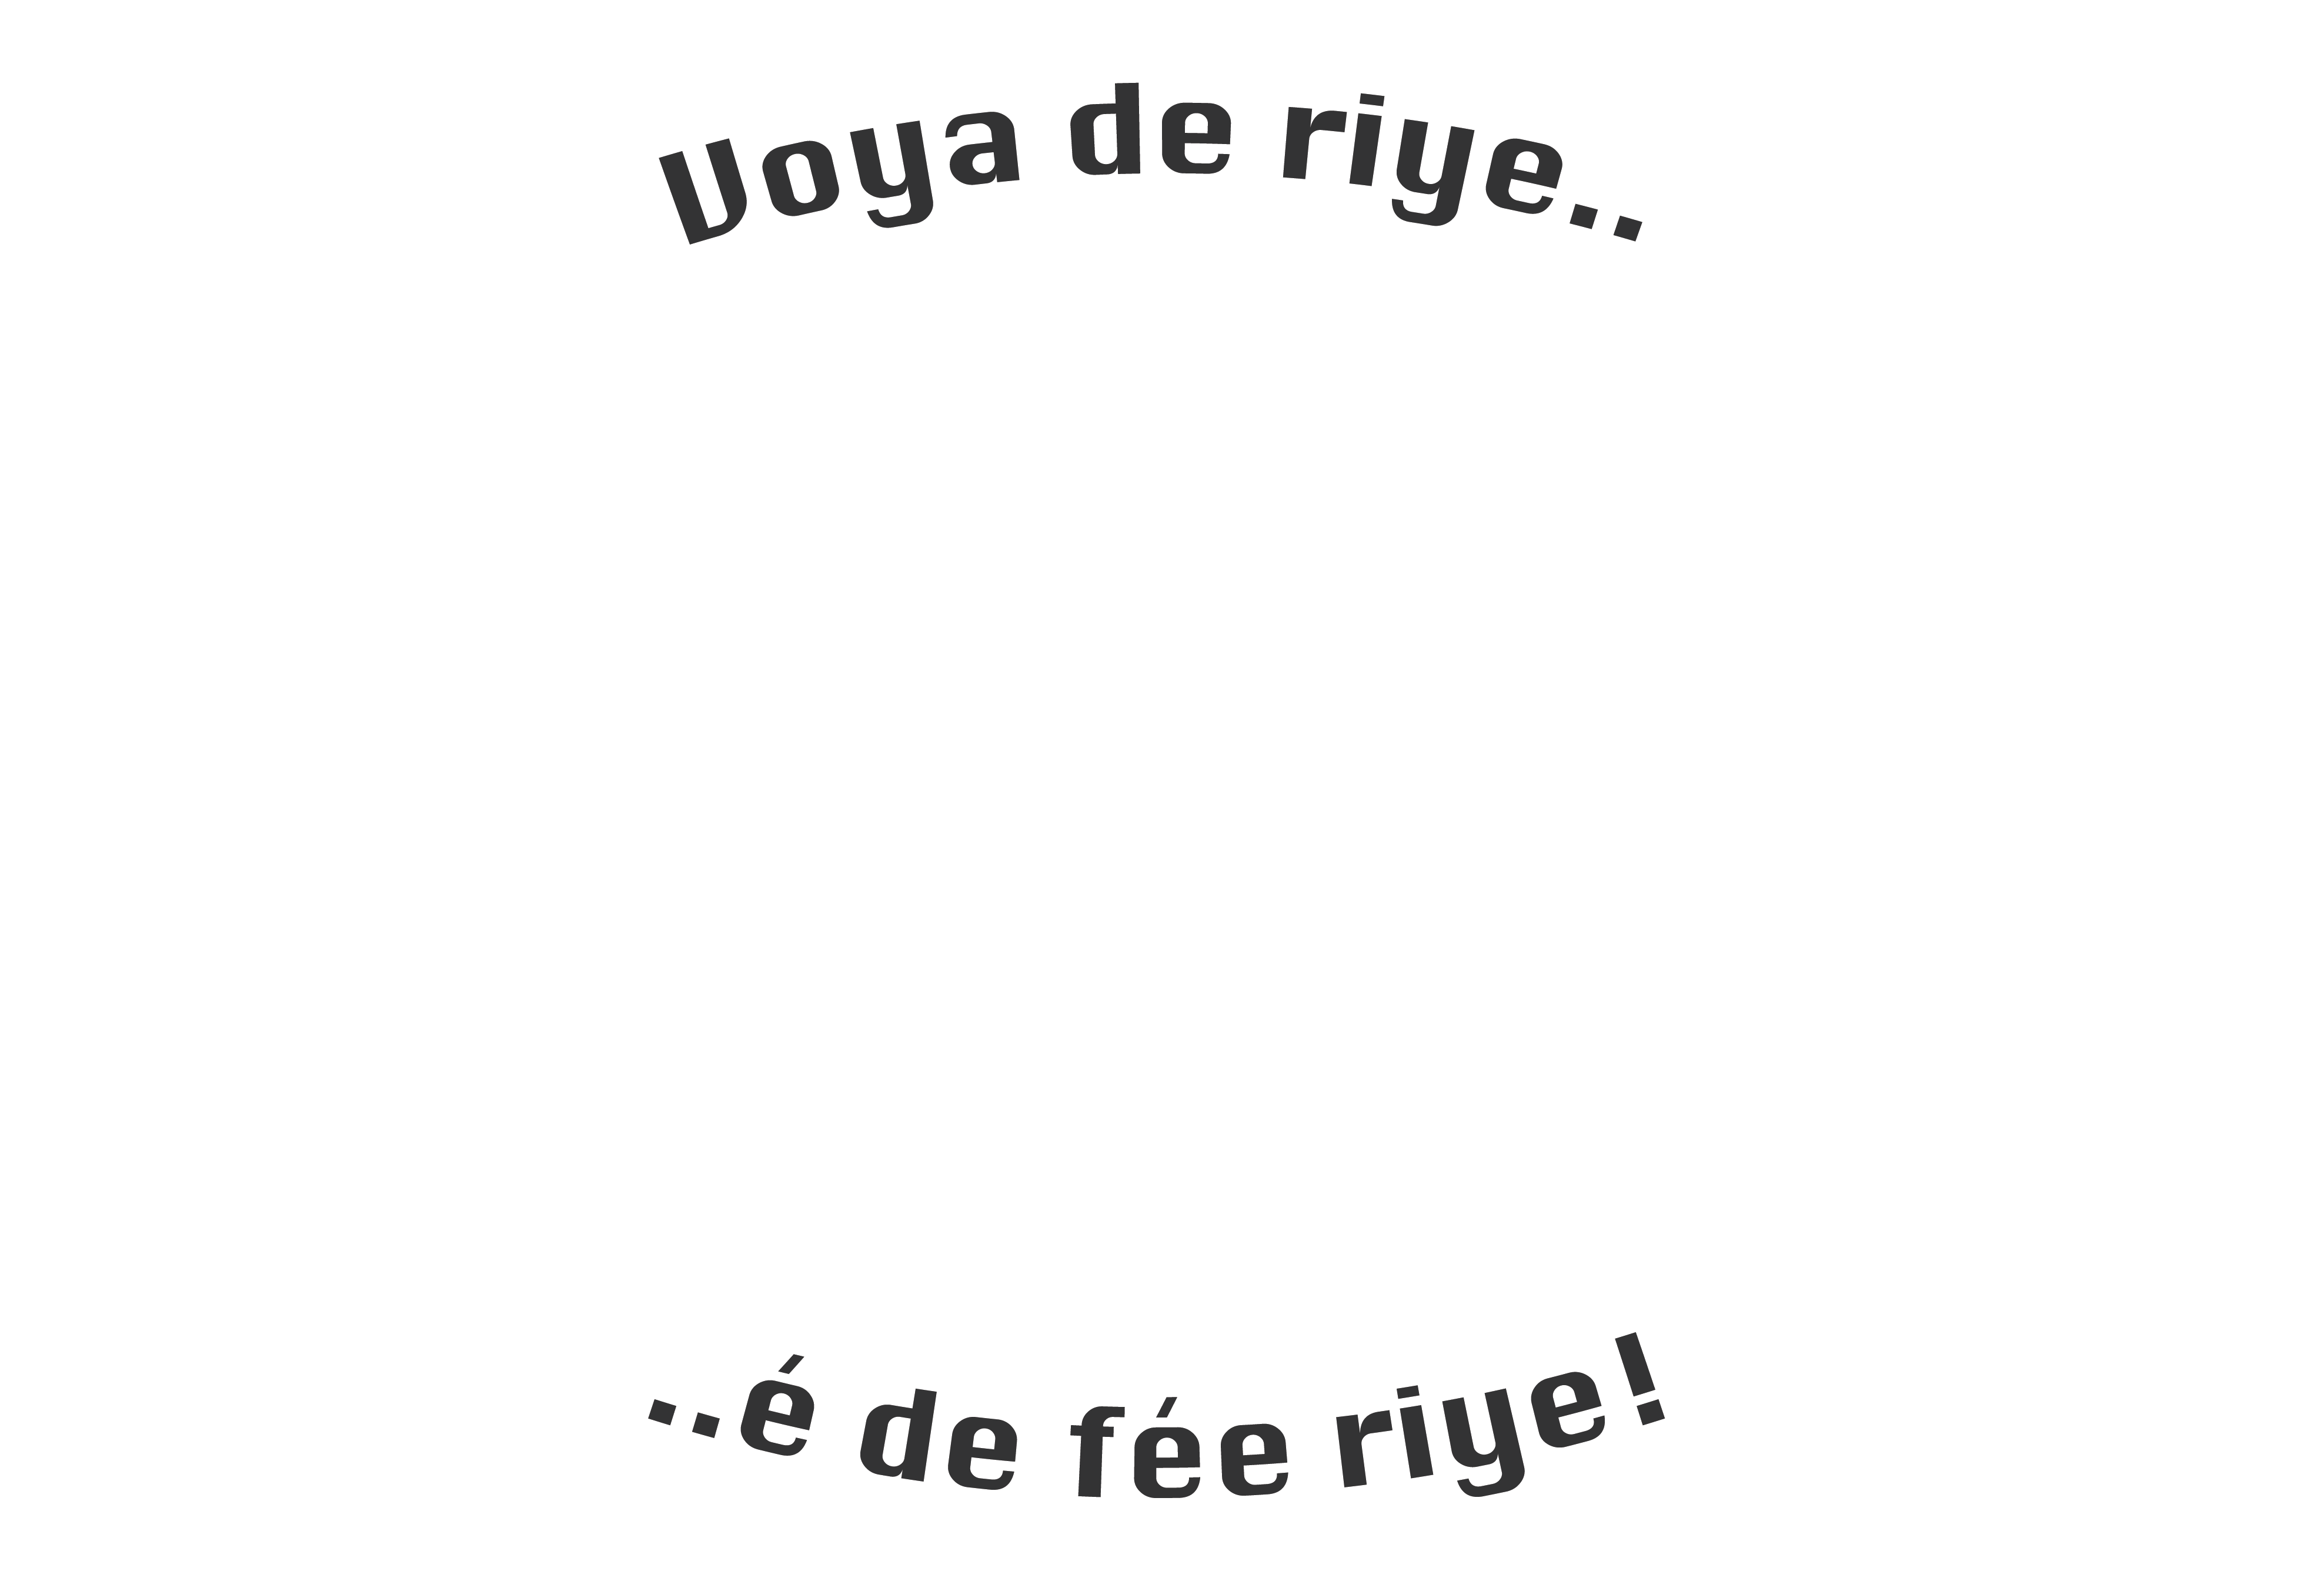
\includegraphics[scale=0.075]{07_official_bianco_stampa.png}\\[0.5\baselineskip] 
%\end{center}
	
	%{\large\textsc{the publisher}} % Publisher
	
	%\vspace{0.1\textheight} % Whitespace under the publisher text
	
	%------------------------------------------------
	%	Bottom rules
	%------------------------------------------------
	
	%\rule{\textwidth}{0.4pt} % Thin horizontal rule
	
	%\vspace{2pt}\vspace{-\baselineskip} % Whitespace between rules
	
	%\rule{\textwidth}{1pt} % Thick horizontal rule
	
\end{titlepage}
\nopagecolor

\clearpage
\restoregeometry
} 

\clearpage
\thispagestyle{empty}
% Ved. p.34 per ordine su dispensa latex (anche per copyright : latex, emoticon)

\chapter*{Colophon} 

\shapepar{\squareshape}{%(vedi computer science per layout colophon)
Si livro l'è it\'o icrì avouì \LaTeX (La(mport)\TeX), eun lojisiel gratouì de compozich\'on \textit{typographique} réalizoù pe Leslie Lamport, que eumplèye \TeX, créach\'on de Donald Ervin Knuth deun lo 1982, comme moteur de compozich\'on.
FONT Nome, autore: "ArsClassica, uno stile
ispirato a Gli elementi dello stile tipografico di Robert Bringhurst"
Le-z-\textit{emoji} FACCINA son it\'o ditsardjà avouì libre lisanse pe lo site \href{https://icons8.com/icons/}{icons8.com}, eun projé a code iver GESTITO/MANTENUTO da ved. COMPUTER SCIENCE....
La COPERTINA di livro l'è itaye réalizaye pe PIPPO é COSA RAPPRESENTA?}
% prendere spunto da colophon della dispensa Pantieri o computer science
\vfill 
\noindent\makebox[\textwidth][c]{%
  \busta\ \href{mailto:jbollon94@gmail.com}{jbollon94@gmail.com}
}
\noindent\makebox[\textwidth][c]{%
  \busta\ \href{mailto:digourdi.tsarvensou@gmail.com}{digourdi.tsarvensou@gmail.com}
}

\newpage 

\clearpage
\begin{center}
\thispagestyle{empty}
\vspace*{\fill}
\Large
\ECFJD
Pe noutra Pach\'on\\
Téatro, Patoué\\
Lenva, \'Emoch\'on\\
rèise de digourdia Amitié
\vspace*{\fill}
\end{center}
\newpage

% pe lo Comédie é lo Patoué
% Istouére é Lenva
% simàn de digourdia Amitié

% cercare di togliere il "de la" 

%%% Indice generale*
\tableofcontents
\clearpage
\listofvideos
\listofsounds
\listofeffets
\listoffotos
\chapter*{Préfach\'on} 
L’aruye po tcheu le dzor, mimo se vo trailledde i Guetsè leungueusteucco, d’eunvian-é eun voyadzo  pai lon é stimulàn a traé d’eun patouè. Patouè d’an quemeun-a mi, euncó de pi, patouè d’an comunitó, euntenduya comme esprèchòn vivanta de eungn eunsemblo de dzi que se recougnison a l’euntor d’eun projè, d’an lenva é d’eun téritouéo. Vouè, péquè le Digourdì son po mocque de brao-z-atteur, son avàn to de dzoun-io Tsarvensolèn, que l’an lo plèizì de pourté su lo palque leur vécù é leur éritadzo, atò l’entouziasme, la frècheur é la voya d’amuzé eun s’amuzèn que l’apartchàn a leur éyadzo.
 
Bièn cheur tsicque jénérachòn eunterprette a sa modda l’éritadzo quemeun. É l’è fran a traé de heutta eunterprétachòn todzor nouila que lo pasó se fa prézèn - attuel é vivàn - é pouze le fondemèn pe l’avin-ì.  Pouchà d’an curiozitó é de eungn’estraordinéa voya de se beté eun djouà, le Digourdì l’an reléó tcheu le défì que lèi son ihó propouzó, eun parcourèn d’an magnî trasversalla de nombreu janre arteusteucco : de la réalizachòn de queurmétradzo eun patouè comme La reconstitution é Là-bas au front, i spettacle final de la 63a édichòn di Concours Cerlogne, eun pasèn pe l’euvra téatralla L’homme au cœur valdôtain dédiéye a la memouî d’Émile Chanoux a l’occajòn di 50o aniverséo de sa mor. Mi étò la produchòn muzicalla, fétte de reprèize de boucòn fameu é de compozichòn orijinelle, é la réalizachòn de nombreu clip vidéó. Le Digourdì prèdzon eun langadzo moderno, frique é ironeucco é lo partadzon su le preunsipal rézó sosial di dzor de vouì : Instagramm, Facebook, YouTube, TikTok, mi étò su de plattefourme muzicalle comme Spotify é Apple Music. 

La Valoda d’Ouha l’areu po pousù espéré de-z-ambasadeur mèilloi di patouè ! 
Pe levré, dz’ouì souligné eungn otro particulié que fa oneur i Digourdì é que témouagne de la maturitó d’an compagnì ioi que l’éyadzo mouayèn di-z-atteur pase po le 25 an : le Digourdì s’eungadzon étò dedeun la formachòn di patouazàn de demàn. Dze penso a l’organizachòn d’ateillì de téatro pe le mèinoù é a la consecanta créachòn, a l’euntèrieur de la compagnì, di grouppe di Pégno Digourdì de Tsarvensoù que l’a débutó su lo palque di Splendor l’an 2023.
Voualà donque eun dzen témouagnadzo de la vitalitó de nouha queulteua é eun motif d’espouer pe son avin-ì.

La publicachòn de hi livro, l’è eungn otro boucòn que se djoueun a an produchòn dza remarcobla. La révijòn di teste l’a demandó an confrontachòn continuella avouì Jordy, é dze crèyo que l’espérianse siye ihéye eunrechissanta pe tcheu dou. Pe mè avàn to que, a traé de l’étsandzo, n’i pousù vivre di dedeun la jénèze di pyihe, eun m’obledzèn a me confronté avouì eun langadzo que évoluye dézò l’eumpulchòn di tsandzemèn que tsicque jénérachòn que lo prèdze pourte avouì sè ; mi, dze crèyo, eunrechissanta étò pe l’oteur, que dz’i vu crèihe di poueun de vuya de l’atenchòn a la lenva é de la métrize de la grafiya.
Eun parcourèn le dji pyihe, lo lèiteur manquerè po d’aprésié l’évoluchòn arteusteucca de la compagnì. Di premî compozichòn que s’ensérèison dedeun la tradichòn populéa pi classeucca canque i teste pi métatéatral de la dérî produchòn.
Eungn ouvradzo complè, an sorta d’antolojì multimédialla di premî dji-z-àn d’an compagnì nèisuya caze pe riye é que avouì lo ten s’et eumpouzéye comme eunna di réalitó pi dinameucque, novatrise é complette di panoramà téatral valdotèn. 

Eun reprègnèn le mo de l’oteur : eun jeste d’amour.
\newline
\newline
\hspace*{\fill} \textit{Daniel Fusinaz}

\chapter*{}
\heartpar{Un grand merci profond et sincère à Daniel Fusinaz, pour avoir cru en cette œuvre, pour la patience et la passion qu'il a déployées dans la relecture de l'ensemble du texte, et pour l'honnêteté intellectuelle avec laquelle il m'a initié à la graphie BREL.
Je remercie également Diego Lucianaz, pour ses conseils, ses suggestions et sa disponibilité sans faille.
Éventuels sponsors à mentionner (?) (Commune de Charvensod, Lucianaz...)}


%Introduzione non numerata
\chapter*{Introduction} 
\markboth{\MakeUppercase{Introduction}}{\MakeUppercase{Introduction}}

%IDEA: APPENDICE CON STATISTISCHE: parole totali, nome più frequente, verbo più frequente ecc.... parola più lunga...; totale e per pièce

% DA QUALCHE PARTE SCRIVERE CHE per i suoni e le musiche c'è un link su soundcloud per trovare ciò che abbiamo creato o salvato. Le canzoni o le sigle non ci sono se non sono state create da noi. Si possono trovare su yt.

% DA QUALCHE PARTE SCRIVERE:  non sono state inserite le indicazione di scena in merito agli ingressi/uscite da dx/sx, se non strettamente necessario... MOtivo: per non appesantire la lettura del racconto con note tecniche di regia.

\paragraph*{Pourquoi Dji Cou Digourdì}
Le recueil Dji Cou Digourdì est né de la nécessité de rassembler toutes les pièces de théâtre interprétées par la compagnie Le Digourdì de Tsarvensoù à l'occasion de ses participation au Printemps Thé\^atral. Presque toujours, les versions finales des textes sont retouchées à la main lors des dernières répétitions, ce moment mystérieux où surgissent, pour une étrange raison, les répliques et les idées les plus drôles, pétillantes et piquantes, et donc les plus efficaces pour l’essor du spectacle. Pour cette raison, les textes théâtraux, archivés quelque part dans les ordinateurs des acteurs, sont restés figés sur une ancienne version du scénario, peu fidèle à la représentation réellement jouée sur scène.

Par ailleurs, les pièces des Digourdì ont souvent intégré au scénario des contenus multimédias: enregistrements sonores, bruitages, vidéos ou images. Ainsi, au-delà de la volonté de témoigner fidèlement des pièces interprétées sur la scène du Printemps Thé\^atral, Dji Cou Digourdì constitue également un archivage des contenus multimédias créés par la compagnie théâtrale \textit{tsarvensolentse}.

Bref, Dji Cou Digourdì s'offre aux lecteurs comme un témoignage vivant et un inventaire précieux de l'art théâtral cultivé par les Digourdì.

\paragraph*{Le contenu}
Dji Cou Digourdì rassemble les dix premières pièces interprétées par la compagnie Le Digourdì de Tsarvensoù à l'occasion de ses participation au Printemps Thé\^atral entre le 2009 et le 2019\footnote{ Au total, cela fait 11 ans ; cependant, en 2017, Les Digourdì n'ont pas participé au Printemps Thé\^atral. La raison de cette absence est expliquée dans le chapitre dédié à l'année 2017.}. Chaque pièce constitue un chapitre et s'articule de la manière suivante :
\begin{itemize}
\item[$\bullet$] Couverture de la pièce avec titre, auteurs, lieu et date de la représentation ;
\item[$\bullet$] Photographie de groupe accompagnée de la liste des acteurs et d'un QR Code pour visionner la vidéo intégrale de la pièce ;
\item[$\bullet$] Entretien avec un acteur, incluant un souvenir personnel et quel\-ques curiosités ou anecdotes liées à la pièce ;
\item[$\bullet$] Description de la scénographie et des principaux éléments de décor utilisés sur scène ;
\item[$\bullet$] Présentation des personnages, dans l’ordre d’apparition, avec le nom de l’acteur qui les incarne ;
\item[$\bullet$] Texte de l’avant-spectacle, le cas échéant ;
\item[$\bullet$] Texte intégral de la pièce ;
\item[$\bullet$] Liste des collaborateurs ayant travaillé en coulisses.
\end{itemize}

\paragraph*{L'habillage}
C'est avec plaisir que je commente également le soin apporté à l'habillage du contenu de Dji Cou Digourdì. J'ai personnellement veillé à ne pas me limiter à la simple rédaction d'un volume réunissant une série de pièces de théâtre classées par ordre chronologique. Étant donné que les Digourdì, depuis leur création, ont toujours cherché à proposer un théâtre novateur, dynamique et créatif, j'ai voulu que ce recueil  reflète cette philosophie à travers une présentation originale, agréable à lire, visuellement attrayante et enrichie d’éléments multimédias.

Pour cela, j'ai choisi de concevoir Dji Cou Digourdì avec \LaTeX, un logiciel gratuit de composition typographique, reconnu pour la qualité exceptionnelle des documents qu’il permet de produire. La grande flexibilité de \LaTeX\ m’a permis d’adapter la mise en page classique d’un script théâtral - pensée à l’origine pour faciliter la lecture par un acteur - en une en une version plus fluide et lisible pour un lecteur intéressé par l’intrigue du scénario. En effet, la beauté d’une composition typographique ne réside pas uniquement dans le texte lui-même, mais aussi dans la manière dont ce texte est disposé : une mise en page réussie sait rester discrète, sobre et cohérente, sans attirer inutilement l’attention ni nuire à la lecture par des espacements incohérents ou des variations injustifiées de style ou de caractère\footnote{ Fazio, Luciano. \textit{Introduzione all'arte della composizione tipografica con LaTeX}. Università degli Studi di Messina, n.d., \url{https://mat521.unime.it/~fazio/tesi/GuidaGuIT.pdf}}. Par conséquent, je suis certain que le lecteur saura apprécier le soin de la composition typographique de \textit{Dji Cou Digourdì} autant que la richesse de son contenu.

Pour apporter une touche de couleur au texte, je me suis inspiré du livre \og Computer Science Distilled: Learn the Art of Solving Computational Problems\fg\footnote{ Waisman, Wladston Ferreira Filho. \textit{Computer Science Distilled: Learn the Art of Solving Computational Problems}. Code Energy LLC, 2017.}, dans lequel les auteurs utilisent des émoticônes pour égayer la lecture de sujets liés à l'informatique. J'ai repris cette idée non seulement pour enrichir visuellement le texte et lui donner une touche d'originalité, mais aussi dans un but didactique: faciliter la compréhension de certains termes ou expressions en patois. Ainsi, le lecteur rencontrera régulièrement des émoticônes représentant un objet, une émotion ou un animal immédiatement après le mot correspondant : \textit{martelette}\martello, \textit{innamoroù}\inamourou, \textit{gadeun}\gadeun.

Enfin, compte tenu de la fonction d'archive de ce recueil, j'ai souhaité rendre facilement accessible au lecteur tout le matériel multimédia produit par les Digourdì au fil des pièces. Grâce à des QR Codes intégrés dans le texte, le lecteur peut accéder directement aux plateformes YouTube, Facebook, Instagram ou SoundCloud pour découvrir les vidéos, les photos, les bruitages et les musiques\footnote{ Les bruitages et les musiques sont accessibles via la version en ligne du présent recueil. Version archivée au sein du dépôt GitHub (voir \hyperref[vers_num]{Annexe - Version numérique}).} réalisés par les Digourdì.

\paragraph*{Méthode}
Maintenant que la raison d'être de Dji Cou Digourdì, son contenu et son habillage ont été clarifiés, il est temps d’en présenter brièvement la réalisation.

La première phase a consisté à rassembler les textes des pièces, sous format papier et/ou numérique, en privilégiant les versions les plus à jour. Ensuite, j'ai entrepris un long travail d’archivage et de visionnage minutieux de toutes les captations vidéo des représentations théâtrales de 2009 à 2019. Ce fut sans aucun doute la phase qui a demandé le plus de temps. En regardant et en écoutant chaque réplique, j'ai mis à jour tous les scripts, en y intégrant également les improvisations - par nature absentes des textes d’origine. De plus, j'ai structuré toutes les pièces en séquence de scènes, chacune dotée d’un titre éloquent.

Une fois terminée la transcription intégrale de toutes les pièces, une phase de révision linguistique a été menée en collaboration avec le Guichet linguistique francoprovençal de la Vallée d’Aoste. Tout le contenu de Dji Cou Digourdì a été corrigé sur le plan orthographique et, du moins en partie, lexical.

En parallèle de ces deux grandes étapes, j'ai aussi collecté l'ensemble du matériel multimédia produit par Le Digourdì\footnote{ Malheureusement, une seule vidéo n'a pas été archivée car elle a été égarée on ne sait où. La vidéo représentait parodiquement la publicité pour l'eau de Santa Colomba « qui, si tu la bois, est une bombe ! » (voir pièce « Eun drolo de distributeur »).} et je l'ai rendu disponible, lorsque ce n’était pas encore le cas, sur YouTube \href{https://www.youtube.com/@the_digourdi}{\yt} pour les vidéos, et sur SoundCloud \href{https://soundcloud.com/user-234168361/sets}{\pppp} pour les bruitages et les chansons.

De plus, pour chaque pièce, j'ai mené un entretien avec un ou plusieurs acteurs afin de recueillir ces souvenirs, anecdotes et émotions qui rendent chaque interprétation unique et irremplaçable. Ces échanges se sont voulus aussi spontané que possible, menés individuellement ou en petit groupe, autour d'un apéritif convivial qui a aidé l'acteur à partager toute son expérience personnelle avant, pendant ou après les représentations.

Je terminerai par quelques notes méthodologiques concernant la scénographie, les costumes, les avant-spectacles et la mention des collaborateurs.
La description de la scénographie vise uniquement à relever les éléments les plus marquants du cadre dans lequel se déploie l’action. Elle s’accompagne d’une liste approximative de certains accessoires de scène utilisés par les personnages. Cette énumération ne se veut absolument pas une reproduction fidèle de la fiche technique détaillée.

Quant aux costumes, j'ai choisi de ne pas leur consacrer une section dédiée. En cas de tenues particulières, celles-ci sont indiquées en note ou dans la description des personnages, lorsque cela s’avérait pertinent.
J'ai également transcrit les avant-spectacles lorsque le script ou l'enregistrement vidéo était disponible\footnote{ En 2014, Jo\"elle Bollon et Laurent Chuc ont chauffé le public avec un avant-spectacle dont, malheureusement, ni le texte ni aucune preuve vidéo n'ont été retrouvés.}. Enfin, j’ai tenu à mentionner, à la fin de chaque pièce, les collaborateurs ayant travaillé en coulisses. Cependant, certains enregistrements de pièce ne comportaient pas les remerciements finaux, j’ai dû m’appuyer sur des photos et des témoignages pour tenter d’identifier les membres de l’équipe. Il est possible que certaines personnes n’aient pas été citées, et si tel est le cas, je l’assure : ce n’est nullement intentionnel !

\paragraph*{Notes stylistiques}
À mesure que le travail avançait, selon la méthodologie exposée dans le paragraphe précédent, j'ai dû faire des choix stylistiques.

Tout d’abord, le patois étant une langue minoritaire, plusieurs mots n'existent pas ou se sont perdus avec le temps. Pour combler ce vide lexical, il est d'usage courant de recourir à des emprunts à la langue française. Toutefois, dans certains cas, j'ai suivi les conseils de Diego Lucianaz, ardent défenseur de Le Digourdì pour le rôle que la compagnie joue dans la diffusion du patois auprès des jeunes générations. Il m'a suggéré de privilégier, lorsque cela était possible, la création de néologismes plutôt que le simple emprunt au français. À titre d'exemple, pour traduire le mot italien « cancelletto (\#) » (dièse en français), j’ai opté pour un néologisme original et adéquat au contexte théâtral : « petchoudacllenda ». Un mot inventé, certes, mais qui, dans le cadre d’une pièce, trouve toute sa légitimité - et qui sait, pourrait un jour entrer dans l’usage quotidien. Un autre exemple : pour « sedia a sdraio » (chaise longue en français) », j'ai proposé le néologisme « caèya di solèi ».
Cependant, chaque fois que la création d’un néologisme n’était pas pertinente ou satisfaisante, j’ai emprunté le terme français correspondant, en l’écrivant en italique. En général, tous les mots provenant d'une autre langue (italien, français, anglais) ont été écrits en italique: \textit{proscenium}, \textit{scène}, \textit{scénographie}.

Les noms propres, en revanche, ont conservé leur graphie d'origine sans italique : Ferrari, Champagne, Facebook, Orage, Pierre, Francesca... Dans ces cas, la première lettre majuscule suffit à signaler au lecteur qu’il s’agit d’un nom propre à lire tel quel, dans sa forme d’origine.

La ponctuation, l'emploi des majuscules, la graphie des nombres en toutes lettres ainsi que les autres conventions linguistiques suivent, en principe, les règles de la langue française.

Un autre aspect très important ayant nécessité une prise de position concerne les nombreuses variantes phonétiques du francoprovençal. Il est connu, du moins parmi ses locuteurs, que le patois varie fortement d’une commune à l’autre, ce qui en fait une langue profondément hétérogène. Pour des raisons évidentes, la variante utilisée dans Dji Cou Digourdì est le patois de la Commune de Charvensod. Cependant, même au sein de cette seule aire linguistique, on y trouve de nombreuses variantes phonétiques : \textit{éve/ive, me plé/me pli, féyo/fio, aprestoù/aprestó}. Face à cette très vaste richesse phonétique, j'ai cherché un compromis entre cohérence et valorisation des variantes qui, à mon modeste avis personnel, représentent une facette précieuse de l'identité de ses locuteurs et méritent d’être conservées. Par conséquent, dans une même pièce de théâtre, le lecteur trouvera le même mot écrit de manière différente. J’ai toutefois veillé à ne pas faire coexister deux variantes en même temps dans une même phrase (\textit{èitsa}/\textit{èita}, \textit{counte}/\textit{conte}).

Par principe, les variantes phonétiques influencées par la langue italienne n'ont pas été retenues, afin de privilégier, chaque fois que possible, l'origine française du terme.

Dernier point, mais non des moindres : la graphie à adopter pour écrire le patois de Charvensod. Jusqu’à présent, j'ai toujours écrit le patois de manière approximative, m'inspirant des règles phonétiques de la langue française et consultant des collègues plus expérimentés. Néanmoins, pour pouvoir publier Dji Cou Digourdì, il me fallait faire appel à quelqu’un en mesure de corriger quelque 450 pages de script. La seule institution en Vallée d'Aoste offrant ce type de révision gratuitement était le Guichet linguistique francoprovençal de la Vallée d'Aoste, qui applique la graphie définie par le BREL\footnote{ Bureau Régional Ethnologie et Linguistique.}. Par conséquent, l'intégralité du texte de Dji Cou Digourdì, a été relue et corrigée selon ces règles. Cette graphie repose sur une logique simple : écrire chaque mot tel qu’il est prononcé, chaque lettre étant porteuse d’un son précis, permettant au lecteur de reconstruire fidèlement la prononciation.

Je n'entrerai pas ici dans le détail des avantages ou limites de cette convention graphique, car il s'agit d'un sujet qui exigerait des connaissances et des compétences bien au-delà des miennes. L'objectif de ce paragraphe est uniquement de justifier le choix stylistique qui a été fait. Un choix dicté par une raison pratique, à savoir la possibilité de faire réviser l’ensemble d’un corpus de 450 pages dans une graphie cohérente et reconnue.

\paragraph*{Un don}
Dji Cou Digourdì n’est pas seulement un travail de mémoire. C’est un geste de reconnaissance envers une communauté, un don offert à Le Digourdì, à son histoire, à ceux qui l’ont fait vivre, à ceux qui en ont ri, applaudi, parfois même pleuré. C’est aussi, profondément, un acte d’amour, car ce recueil m’a demandé une quantité de temps incalculable — et le temps donné c’est la forme la plus pure d’amour.
\newpage
\begin{center}
Il ne me reste plus qu'à vous souhaiter une\ldots\\\vfill bonne lecture !\\\vfill\#todzorpidigourdì
\end{center}

%Dji Cou Digourdì est un don offert à Le Digourdì, à son histoire, à ceux qui l’ont fait vivre, à ceux qui en ont ri, applaudi, parfois même pleuré. C’est aussi, profondément, un acte d’amour. Car ce projet m’a demandé une quantité de temps incalculable — et le temps donné, c’est la forme la plus pure d’amour.
%Dji Cou Digourdì n’est pas seulement un travail de mémoire ou un objet éditorial. C’est un geste de reconnaissance envers une communauté, un patrimoine, une langue fragile mais tenace. C’est ma manière de rendre ce qui m’a été transmis, de remercier par l’écriture, la recherche, l’écoute, et de faire durer ce qui, autrement, pourrait s’effacer.
%Ce projet est en lien avec une tradition vivante que je suis fier d’avoir, peut-être, contribué à faire perdurer.





\mainmatter

%\title{L’OPETAILLE MODERNO}
\author{Pièse icrita pe Jo\"{e}l Albaney}
\date{Téatro Giacosa de Veulla, 15 mi 2009}

\maketitle

\fotocopertina{Foto/2009/gruppo_red.jpg}{Paola Lucianaz, Francesca Lucianaz, Jo\"{e}l Albaney, Jasmine Comé, Paolo Cima Sander, Giada Grivon, Paolo Pession, Pierre Savioz, Ilaria Linty}{Valeria Brunod, Serena Giorgi, Jo\"{e}lle Bollon, Simone Roveyaz, Laurent Chuc, Ester Bollon, Marco Ducly}{2009}\label{link}

\LinkPiese{L'opetaille moderno}{https://www.youtube.com/watch?v=lP22_oK_hws&list=PLBofM-NS_eLJUln45l7VH457fGak_Bk5O&index=10}{.5}

\souvenir{Mon souvenir de l'Opetaille moderno l'è, sensa doute, salla sensach\'on que sayò eun tren de vivre eun sondzo, eugn'émoch\'on euncrouayable. L'ie lo premì cou que noutra compagnì, djeusto nèisiya, pouyè si eun vrèi palque\ldots é lo fé que si palque l'ie fran lo Téatre Giacosa, \textit{symbole} di téatro populéro valdotèn, l'ie eunna \textit{source} pouissante de jouà é responsabilitoù. Dze n'i eun dzen souvenir pe la collaborach\'on que n'en i avouì lo Charaban, eun particulié avouì Vittorio Lupi, Mauro Rossi é Giovanni Neri. L'an fé-no découvrì comme s'apreste a niv\'o professionnel eun spectaclle téatral, sourtoù pe sen que regarde la \textit{scénographie} é le costume. Me rappelo avouì plèizì que Aldo Marrari l'ayè chouivino deun la produch\'on de totta la pièse.

Deun mon \textit{cœur} l'Opetaille moderno l'a cheur eun caro eumpourtàn, pequé l'a dimoutro-me que n'a ren de pi dzen que traillì avouì de dzi é de-z-amì que l'an la mima pach\'on de té.}{Jo\"el Albaney}

%
\queriaouzitou{
\begin{itemize}

\item[$\bullet$] La \textit{scène} di maladdo \textit{psychiatrique} l'è itaye eumprovisaye deun la dériye proua jénérale sensa que Ester diise ren a gneun! Pouade imajiì la réach\'on é le riaye de totta la compagnì.

\item[$\bullet$] Lo Téatre Giacosa de Veulla l'a lo palque eunna mia dicllo ver lo pebleuque. Donque, tcheu le-z-objé avouì de raoue dèyon itre blocoù pe pa colaté. Malereuzamente, d'eunna \textit{scène} avouì bièn de trimadzo, le fren di raoue de la coutse de Geromine son digantsa-se. Bièn aloù que noutro Paolo Cima Sander l'è arrevoù  a vardé lo pèise de la coutse que l'ie eun tren de colaté ver lo pebleuque! Queriaou de savèi pe queunta \textit{scène} capite? Alade la tsertchì deun la \textit{vidéo} de la pièse\footnote{ QR code a padze \pageref{link}}.

\item[$\bullet$] Pe la pièse l'Opetaille moderno le Digourdì l'an rejistroù leur premiye parodì d'eun \textit{refrain} publisitère: \og Di Congo pe travaill\fg. La publisit\'o orijinelle l'è seutta:

\begin{figure}[H]
%\vspace*{-5pt}
\centering
      \begin{subfigure}{.75\textwidth}
  \centering
    \video\hspace*{0.5mm} \textsc{\small Bollywood TVC - Rio Casa Mia}\hspace*{0.5mm} \video\\\vspace*{2mm}
    \qrcode[hyperlink, height=0.5in]{https://www.youtube.com/watch?v=EoVlYvr5JbI}
  \end{subfigure}%
\end{figure}

\item[$\bullet$] Sel\'on lo premì Prézidàn di Digourdì, Jerome Saccani lamè traillì derì le rid\'o pe pouèi veure le dzente feuille de la compagnì totte eun ganeuss\'on!
\end{itemize}
}

\Scenographie
\begin{itemize}
\item[$\bullet$] 2 coutse d'opetaille é 1 coutse a doe plase bièn comodda \lettodoppio ;
\item[$\bullet$] 3 \textit{tables de nuit};
\item[$\bullet$] 2 armouére;
\item[$\bullet$] 2 caèye nèye eun plasteucca ;
\item[$\bullet$] 1 pourtamantì;
\item[$\bullet$] 1 poltronna bièn comodda;
\item[$\bullet$] 1 fondal téatral avouì eunna pourta i mentèn pe laquella le-z-atteur pouon entré é chotre;
\item[$\bullet$] 1 bourset pe le grou sou é 1 pe le sou tri;
\item[$\bullet$] 1 campaneun \campanellino ;
\item[$\bullet$] 3 botèille de \textit{gatorade} ;
\item[$\bullet$] 1 flute ;
\item[$\bullet$] 2 cabaré d’ardzèn: 1 pe pourtì eun \textit{cracker} é l'atro pe la cachoula de la \textit{bourguignonne} ;
\item[$\bullet$] 1 per de motchaou;
\item[$\bullet$] 2 platte de papì, de fortsette é de caoutì \posate ;
\item[$\bullet$] 2 cachoule: eunna grousa pe fé la puré é l'atra pi pégna pe fé bolequé  l'ouillo de la \textit{bourguignonne};
\item[$\bullet$] 1 vèyo é 1 paille.
\end{itemize}

\setlength{\lengthchar}{3.25cm}

\Character[PIERRE]{PIERRE}{Pierre}{Premì prézentateur, \name{\\Pierre Savioz}}

\Character[LAURENT]{LAURENT}{Laurent}{Sec\'on prézentateur, \name{\\Laurent Chuc}}

\Character[GEROMINE]{GEROMINE}{Geromine}{Eunna viille madama\ \viille\ recovéraye a l'o\-pe\-taille, \nameF{Jo\"{e}lle Bollon}}

\Character[CASIMIR]{CASIMIR}{Casimir}{Vétchot \viou\ campagnar  recoveroù a l'opetaille, \name{Jo\"{e}l Albaney}}

\Character[ARISTOCRATE]{ARISTOCRATE}{PersEmpourtanta}{Mesieu bièn eumpourtàn, noble é aristocrate, recoveroù a l'opetaille, \name{Marco Ducly}}

\Character[GASTON]{GASTON}{Eunfeurmi}{L’eunfermì personnel de l'Aristocrate, \name{Laurent Chuc}}

\Character[PRIE]{PRIE}{Prie}{Lo prie de l'opetaille \prete , \name{Pierre Savioz}}

\Character[FENNE\\ DI POULISIE]{FENNA DI POULISIE}{Fennepulisie}{Femalle arbeillaye comme le méccanisièn de la \textit{Ferrari}, eunterprétaye pe \textsc{Jasmine Comé}, \textsc{Giada Grivon} é \textsc{Serena Giorgi}. Giada é Jasmine feràn eunc\'o le-z-eunfermiye de la \textit{psychiatrie}.}

\Character[STARTER]{STARTER}{Starter}{Cape di fenne di poulisie, \name{\\Simone Roveyaz}}

\Character[EUNFERMIYE]{EUNFEURMIYE}{Eunfeurmie}{Eunfermiye de l'opetaille avouì eun caratéo d'eun maréchal, \nameF{\\Francesca Lucianaz}}

\Character[JOSETTE]{JOSETTE}{Felie}{La feuille de Geromine, \nameF{\\Ilaria Linty}\\}

\Character[MEDESEUN\\ MITCHO]{MED. MITCHO}{MedMitcho}{Lo \textit{Doctor House} de l'opetaille, \name{Paolo Cima Sander}}

\Character[FERNANDA]{FERNANDA}{Fernanda}{Lo Chef de l’opetaille, \nameF{Ester Bollon} Ester ferè eunc\'o lo maladdo \textit{psychiatrique}.}

\Character[TSAMBR\`I]{TSAMBR\`I}{Tsambri}{Tsambrì personnel de l'Aristocrate, \name{Pierre Savioz}}

\Character[]{FENNA DI POULISIE I}{FennepulisieA}{\hspace*{0cm}}
\Character[]{FENNA DI POULISIE II}{FennepulisieB}{\hspace*{0cm}}
\Character[]{FENNA DI POULISIE III}{FennepulisieC}{\hspace*{0cm}}

\DramPer

\act[\avanSpect\ Avanspettaclle \avanSpect]
\StageDir{\hspace*{2.5em}Se senton de vouése que veugnon de dérì la tèila.}

\begin{drama}

\Pierrespeaks Laurent entra té, mé n'i pouiye.

\Laurentspeaks Pouiye? Feulla!

\Pierrespeaks \direct{Ajitoù\ajitou} Soplé va té!

\Laurentspeaks T'i tan grou é t'a pouiye de cattro personne que son vie no vére?!

\Pierrespeaks Ad\'on fièn na baga? Baillèn dou creppe a la moura!

\StageDir{Le dou fan eunna man a la moura (\og tchisse, cattro, totta man, satte\ldots \fg ).}

\Laurentspeaks Ah! Pierre, deusteun! Feulla!

\Pierrespeaks\direct{Eun prégnèn coadzo} Ad\'on vou mé!

\StageDir{Lemie \lemieSi\ desù lo \textit{proscenium}. Pierre chor de dérì la tèila.}

\Pierrespeaks Bonsoir a tcheutte!

\StageDir{Entre eunc\'o Laurent é se plache a drèite de Pierre.}

\Pierrespeaks\direct{A Laurent} Mondjemé véo de dzi oueu lo nite! N'ayoù pa la fèi tan pai!

\Laurentspeaks\direct{Eun avèitsèn lo pebleucco} N'ayoù pa la fèi tan pouèi!

\Pierrespeaks A mé l'ay\'on deu-me que dèi seu desù lo palque te vèyave ren de sen que capitae déz\'o lo palque! \direct{Ajitoù} Mi me semble pa! Se vèi totte!

\Laurentspeaks Eh ouè! Mi se t'avèitse amoddo trèi car de la sala son pa de Tsarvensoù!

\Pierrespeaks T'a rèiz\'on! Can mimo\ldots a Fin-is l'an pi eunc\'o de dzente feuille! \`Eita salle do lé eun premì feulla!

\StageDir{Laurent seuble i feuille.}

\Pierrespeaks Mi va savèi péqué n'a pi de dzi de Fin-is oueu!

\Laurentspeaks Pierre! Avouì tcheu le tracasse que le Tsarvensoulèn l'an i dzor de oueu, fegueua-té se l'an lo ten de vin-ì sé pe avèitchì no!

\Pierrespeaks T'a rèiz\'on! Son tcheu pi greundzo\ldots pe deue\ldots té pensa que eun cou t'ayè praou te réchì a satte é demì pe alé eun Veulla a ouètt'aoue. Ara, avouì seutta dzenta arionda que l'an fé-no ba i Pon-Suà te fa te réchì a chouì é demì! Péqué eun cou que t'i  ba, te fa baillì la présédanse i Gressaèn; aprì pi de 50 an que n'en i no si drouette! \'E comme se bastise pa, can te feullon devàn l'an eunc\'o eun grou sourì a 32 di \sorrisone .

\Laurentspeaks T'a rèiz\'on! Aprì te fa eunc\'o chotre demì aoua devàn di travaille pe alì a l'icoula prende le botcha é alì i mitcho pe fé medjì!

\Pierrespeaks Mi na! Senque te me di? L'è pa lo travaille di-z-ommo sitta! Son le fenne que dèyon pensé i megnadzo!

\Laurentspeaks \direct{Ironique} Eh brao! Eun cou l'ie pouèi! Aya a Tsarvensoù, dèi can la betoù si do formach\'on di femalle di fiolet, leur pi grou tracasse l'è si d'aprestì l'èima, baillì la biacca i fiolet é prenotì le campe réjonal pe la demendze.

\Pierrespeaks Ouè, ouè\ldots sitta cou va fran tott'a bal\'on!

\Laurentspeaks Te pou pa resté avouì seutta vya! T'i stressoù! Aprì fenèi que eun se beutte maladdo!

\Pierrespeaks Queutta pédre! Te la sa la dériye?

\Laurentspeaks Di-mé.

\Pierrespeaks Noutro Senteucco, Ennio Subet, dèi can l'a si qué que lo Ministre Brunetta l'è fé-se eunna loué si lo travaille, l'a voulì eunc\'o llou fé la sin-a.

\Laurentspeaks N'ayò sentì de seutta loué: la \textit{Subettina}. Espleucca vèi comèn fonchoun-e!

\Pierrespeaks Ad\'on, te sa que Brunetta l'a desid\'o d'aoumenté l'oréo de la \textit{mutua}; donque, lo noutro Senteucco la betoù na riilla pe tcheut le sitouayèn! Dèi ara can eun l'è maladdo, l'è maladdo i $100\%$! Te pou gnenca pamì alì ba a la crotta pe prendre eunna boua botèille de veun ou alì de foua pe couillì le pomme \mela .

\Laurentspeaks Ah ara n'i comprèi péqué l'è na senâ que vèyo pa lo meun vezeun di mitcho é pe tèra n'at totte le pomme pouriye.

\Pierrespeaks \ldots é fa fé attench\'on! Péqué lèi  son le vallet de veulla que pasoun, dzor é nite, mitcho pe mitcho pe verifiì. An effè, l'an pamì lo ten de pasì i mentèn de la parotse pe baillì la multa i machine parquédjaye mal!

\Laurentspeaks \ldots é comme se n'isse panco praou, n'a eunc\'o d'atro mé cher-z-amì, péqué eun cou que t'a aprést\'o sin-a, t'a baillà medjì i mèinoù é t'a lav\'o le-z-éze\ldots te l'amerie pa t'itaoulé eun momàn desù lo chofà pe avèitchì lo \textit{Grande Fratello}?

\Pierrespeaks Ouè!

\Laurentspeaks Eh na! Péqué totte le souaré, can si preste m'achouaté si lo chofà lo tseun comenche a djapì é molle pa tanque lo pourto pa féye eun tor deun lo péi!

\Pierrespeaks Mi senque te me di? Itèn pa pe eunna grousa Veulla! T'a praou baillì campa a la tsèin-a é lo tor se lo fé da solette!

\Laurentspeaks A Tsarvensoù?! Mi t'i matte! Fenèi que lèi teurion desì avouì lo fezì!

\Pierrespeaks Me rappelao pamì de seutta counta! \'E t'a sentì que n'at eunc\'o la finanse é le carabignì di bouque que son eun tren de cayì to pe l'er lo péi pe tchertchì seutte-z-arme?

\Laurentspeaks N'ay\'o sentì de seutta counta; é say\'o tellemàn tracachà que n'i falì euntéré deun lo courtì le dou pistolet a éve: le dou \textit{Super Liquidator} di botcha!

\Pierrespeaks Acouta vèi seuilla.

\StageDir{Laurent s'aprotse.}

\Pierrespeaks \direct{Eun moutrèn quetsouza déz\'o la djacca} Te vèi lo pistolet a éve que n'i seuilla?
Me fa todzor lo pourté aprì\ldots l'è pa denonchà.

\Laurentspeaks Oh pouff, que viya! No n'en eunc\'o baillà lo non Digourdì a noutra compagnì!

\Pierrespeaks Ouè que coadzo!

\Laurentspeaks  Spéèn que le tréze que son séilla dérì \direct{moutre la tèila} teugnon pi ate lo non di groupe!

\Pierrespeaks Can mimo douàn can sen chortì di tend\'on n'ay\'on tan pouye di dzi\ldots ara n'en finque prèi tro de coadzo.

\Laurentspeaks N'en eunc\'o prao deu-nen! Spéèn can mimo que la quemeua é tcheutte le Tsarvensolèn contenisa no baillì na man; piatro sit an l'è lo premì é dérì an que fièn lo \textit{Printemps Thé\^{a}tral}.

\Pierrespeaks Ouè! \direct{Eun avèitsèn la moutra \orologio} Ara senque te nen di se prézentisan la pièse?

\Laurentspeaks \direct{Eun avèitsèn lo seun pouse sensa moutra \footnote{ Malerezamente Laurent l'è oublia-se de betì la moutra, mi lo pebleucco l'a bièn riette pe seutta gaffe.}} Ouè l'è l'aoua de comenchì, mi devàn vourio fé na présizach\'on pe tcheu le Tsarvensolèn: tcheu sise manifeste que n'en bet\'o ia pe la parotse, l'è pa pequé gavon l'éve ou l'élétrisit\'o, mi l'è pe lo spétaclle de seutta nite! Tracachade-v\'o pa!

\Pierrespeaks Amoddo! Mogà no sistémèn an miya pe la prézentach\'on?

\StageDir{Pierre é Laurent se cllouzon la djacca é drichon lo papillon \papillon . Eun pi, Laurent se beutte si le poueunte di pià é Pierre se plèye si le dzegnaou de fas\'on que sisan ate tcheut dou igale.}

\Pierrespeaks \textit{Mesdames} é \textit{Messieurs} a vo \og L'opetaille moderno\fg . Pise icrita pe Jo\"{e}l Albaney.

\Laurentspeaks Boun-a souaré a tcheut!

\StageDir{Pierre é Laurent chorton. Teuppe \lemieBa .}

\act[Acte I]
\pagestyle{headings}

\ridoiver

\scene[-- L'Aristocrate é le pouo matasse]

\StageDir{Partèi la tsans\'on:}

\sound{https://www.youtube.com/watch?v=cntvEDbagAw}{A Message to You Rudy - The Specials}

\StageDir{Eun \textit{scène} n’a trèi coutse. Doe coutse, salle iaou son itaouloù Casimir é Geromine, son bièn seumple é protso n'a maque doe caèye é doe \textit{tables de nuit}; i contréo, la trèjima coutse (a gotse) salla de la personna eumpourtanta l’è d’ott\'on, queusseun de sèya, \textit{couvre-lit} avouì le frandze. Acoutì n'at eunna comodda poltronna é eunna \textit{table de nuit}. Pe completì la \textit{scénographie}, i fon di palque n'a dou-z-armouére eun feur, eun pourtamantì é eun grou fondal avouì eunna pourta i mentèn.\\ L'aristocrate l’è catchà déz\'o le queverte é l'è eun tren de drimì. Geromine l’et eun tren de fé lo tsaous\'on é lo vioù l’et eun tren de lie lo journal avouì le lenette ba desì lo na.}

\StageDir{Se sen pamì la tsans\'on.}

\Gerominespeaks \direct{A Casemir} L’è na senâ que si seuilla dedeun é si pa senque atègnon a me fé chotre.

\Casimirspeaks T’atten pi eunc\'o té comme tcheutte!

\Gerominespeaks Si pi praou coudzia. Mi mé sensa lo meun courtì é le mie dzeleunne \gallina\ si perdiya!

\Casimirspeaks \direct{Euntre lli} Eunna pi, eunna mouèn\ldots

\Gerominespeaks N’i pa comprèi\ldots senque t’a deu?

\Casimirspeaks Ren, ren! Diavo maque que te pouave te le porté avouì té! Omouente n’ario magà pouì féye de nouo discour avouì caqueun. Le-z-aoue comenchon itre londze seuilla dedeun\ldots é lo spettacllo l’et todzor lo mimo \direct{avouì lo dèi moutre \deidreite\ Geromine} é ta viya la si perqueue: l’è chouì cou que te me la conte!

\Gerominespeaks Te pense que a mé fiyisse plèizì restì seuilla avouì eun rabadàn comme tè? Surtoù veure, can te tsandzon le fise, eun moustre patanì pi é ouse, blan comme lo lasì é sensa pamì ren de euntéressàn pe le femalle.

\Casimirspeaks Magara pe de femalle comme té! Se le femalle que travaillon seuilla son jantile maque avouì mé n’aret eunna rèizón! \'E té te fa pa itre dzalaouza! \'E aprì resta maque tranquilla, itsauda-té pa\ldots piatro te pren eugn atro \textit{infarto}!

\Gerominespeaks Mé ara resto adì bièn é si pa senque baillerio pe itre eun campagne.

\Casimirspeaks Ouè fa beun diye que s’en eun trèi malado eun tsambra é l’atro \direct{moutre la personna eumpourtanta} l’a panco t’an prédzà.

\Gerominespeaks Ouè ren! S’en gneunca lo non. Se n'i comprèi a\-mod\-do dèi itre euna grousa tita.

\Casimirspeaks Eh vouè, t’ayè panco comprèi-lo? Mi te avèitse pa lo TG3? Sitte l'é tcheu le momàn eun télévij\'on \tv . Eun dzor pe an bagga é eun dzor pe eugn'atra.

\Gerominespeaks Na. Mé acouto maque la \textit{Voix de la Vallée} desù la radi\'o \radio .

\Casimirspeaks Ad\'on l’é l’aoura que te te modernizisse an miya!

\Gerominespeaks Mé reusto bièn pai: de ouette a onze se si i mitcho \textit{Radio Zeta} avouì Ciccetti é a maenda lo \textit{Gazzettino}, avouì Cesarino!

\StageDir{Se rèche l'aristocrate que l’ie eun tren de drimì. Se derèidì é aprì pren lo campaneun \campanellino\ pe querì lo seun valet.}

\PersEmpourtantaspeaks Gaston! Gastooon!

\StageDir{Entre Gaston.}

\Eunfeurmispeaks Bondzor mesieu! Sade dza réchà?

\PersEmpourtantaspeaks Djaque!  Queun dzor l'é oueu? 

\Eunfeurmispeaks Oueu l'è devendro 15 Mi. L'è onj'aoure é sinque di mateun, lo ten l'è séèn é eun Val d'Outa l'è pa capitoù ren d'eumpourtàn.

\PersEmpourtantaspeaks Amoddo, ad\'on refèicha-mè djeusto le queverte.

\Eunfeurmispeaks To de chouite!

\StageDir{Gaston gnouye refèichì le queverte.}

\PersEmpourtantaspeaks Tro itrèite! 

\Eunfeurmispeaks\direct{Eun refèichèn} Va mioù pouai?

\PersEmpourtantaspeaks Tro lardze!

\StageDir{Gaston moungouye eunc\'o eun momàn.}

\Eunfeurmispeaks Va bièn ara?

\PersEmpourtantaspeaks Ouè va bièn.

\StageDir{Lo vioù, que l'a vi la \textit{scène}, l’a i fon de la coutse le queverte beuttaye mal é lo toppon pa totte. Ad\'on pe pa trebelì proue a se fé èidjì.}

\Casimirspeaks Gaston! Squezade Gaston! 

\StageDir{L’eunfeurmi fé semblàn de ren, ad\'on lo vioù tourne lo criì eun vouaillèn.}

\Casimirspeaks Deh, Squezade! 

\Eunfeurmispeaks Ouè.

\Casimirspeaks Me refèichade la coutse i fon pe plèizì?

\Eunfeurmispeaks Mi squersade pa mesieu, pouì pa vegnì tanque lé! Aprì qui reste seuilla a avèitchì lli?

\Casimirspeaks Que demanda foula que n’i fé. L’é vrèi n’ayoù pa pensou-lèi.

\StageDir{Se viounde di coutì de la viille é sopatte la tita.}

\scene[-- Le sen-z-ouillo]

\StageDir{Entre, de la pourta i fon di palque, eun prie tot arbeillà de neur, avouì la Bible eun man.}

\Priespeaks\direct{Eun fièn la croueu} Bondzor a tcheutte.

\Casimirspeaks Bondzor Monseur.

\StageDir{Lo prée s'aprotse a Gaston, que l'ie eun tren de poulitì le-z-onlle de l'aristocrate.}

\Priespeaks Mesieu\ldots

\Eunfeurmispeaks Ouè.

\Priespeaks \ldots qui l'è lo pi vioù é pi maladdo seuilla?

\Eunfeurmispeaks \direct{Eun moutrèn Casimir}
L'è si lé!

\Priespeaks Mersì.

\StageDir{Lo prie s'aprotse a la coutse de Casimir é dousemàn, avouì bièn de pitié, lèi fé la croueu \croce\ si lo fron.}

\Casimirspeaks\direct{Eun branquèn lo bri di prée} \'E so?! Que fiade? Mi squersade pa!

\Priespeaks \direct{Eun lèi prédzèn comme fuse eun pouo matasse} Mesieu, comme la demando-me voutra fameuille si vin-ì vo saliì pe lo dérì cou.

\Casimirspeaks \direct{Eun se totsèn le-z-attribus} Mi na na! Que fiade? Si pa preste a moueure mé!

\Gerominespeaks Mi senque te te totse? N'a pamì ren lé \riye !

\Casimirspeaks Ah! souplì là!

\Priespeaks \direct{\'Eton-où \ouaou} Comèn?! Mi seutta l’è pa la tsambra numer\'o 17?

\Casimirspeaks Na, na seutta l’é la tsambra nimér\'o\ldots \direct{se veurie ver Geromine} nimér\'o?

\Gerominespeaks \direct{A basa vouése} 23.

\Casimirspeaks Seutta l’è la 33!

\Gerominespeaks \direct{Eun vouaillèn} 23!

\Priespeaks Boundjeu de la France! Squezade-mé tan! Si fran trom\-pou-me! Ad\'on me fa belle partì, piatro me scappe finque lo mor!

\StageDir{Baille la bénédich\'on a la tsambra é can l'è preste a chotre tourne eun derì ver Casimir.}

\Priespeaks Mesieu, si pa se v'ouèide sentì que no fa refé lo tette de l’éillize. Se vouillade pouade fé can mimo eunna queilletta pe l’éillize\ldots

\Casimirspeaks Na mé n'i dza baillà proou a meun ten.

\Priespeaks\direct{Diplèizì} Ah. \direct{Ver Geromine} Vo madama?

\Gerominespeaks Me deplì, mi mé se dérì n'i pa lo boursette. Pi que de bot\'on n'i pa.

\Priespeaks Fé pa ren ad\'on. Fé pa ren. Tracachade vo pa.

\Casimirspeaks Acoutade na baga: \direct{eun moutrèn la personna eumportanta} deumandade a llou que nen n'a d’avanse!

\Priespeaks Ah mersì bièn.

\StageDir{Lo prie va ver l'aristocrate.}

\Priespeaks\direct{A Gaston} Bondzor mesieu. Poui-dz\'o lo réchì?

\Eunfeurmispeaks Eh na, l'è eun tren de drimì. L'è mioù que lo rècho mé.

\Priespeaks Va bièn. Vito que n'i prisa.

\StageDir{Gaston to todzèn tsertse de réchì lo seun mesieu.}

\Eunfeurmispeaks\direct{Eun totsèn la man a l'aristocrate} Mesieu. Mesieu\ldots

\StageDir{L'aristocrate se rèche pa.}

\Priespeaks \ldots squezade. Mi n'i fran prisa. Lèi penso mé.

\Eunfeurmispeaks Va bièn, comme vouyade.

\StageDir{Lo pri beutte eunna man si l'ipala de l'aristocrate.}

\Priespeaks\direct{Eun braillèn} Mesieu!

\StageDir{L'aristocrate se rèche épouvant\'o .}

\PersEmpourtantaspeaks Ah! Eh! Oh, senque?!

\Priespeaks Bondzor.

\PersEmpourtantaspeaks Salì!

\Priespeaks Mesieu l’an deu-me que v'ouèi de voye moustre de fé de bienfezanse pe l’éillize.

\PersEmpourtantaspeaks Oué\ldots \direct{Ver Gaston} va prende lo bourset.

\StageDir{Gaston pren lo bourset di mesieu é teurie foua bièn de sou \cash . Lo mesieu lèi di de na avouì la tita; ad\'on Gaston nen teurie foua eugn atro pi petchoù é lo mesieu tourne lèi diye de na.}

\Eunfeurmispeaks Monseur n'i pa de tri. Vou a vére pe lo bourset di pise.

\StageDir{Gaston tourne eun derì avouì eun per de sou tri eun man.}

\Eunfeurmispeaks N'i acap\'o so!

\StageDir{Gaston baille i prie le dou tri que l'a prèi pe lo bourset.}

\Priespeaks Oh mersì. \direct{Ironique} V'ouite fran itoù jantilo.

\Eunfeurmispeaks Mersì a vo.

\Priespeaks Oueu lo nite fiyo eunna prière pe tcheu vo é tourno vo troué demàn mateun. Repouzade-v\'o. Orvouar a tcheutte.

\StageDir{Lo prie fé la marca de la croueu é chor.}

\scene[-- Ferrari \ferrari\ poulisie]

\StageDir{Entron trèi femalle di poulisie: son arbeillaye avouì eun tone rodzo de la Ferrari. Eunna avouì l'icaoua \scopa , l’atra avouì de prodouì pe poulitì é la dérie avouì eun tchappapoussa.}

\Fennepulisiespeaks Bondzor a tcheutte!

\Casimirspeaks \direct{Eun fièn vère que l’è to contèn} Bondzor! Voualà l'è dza torna aoura di poulisie!

\FennepulisieAspeaks Bièn lévoù?

\Gerominespeaks Mi ouè, mersì, é vo?

\FennepulisieBspeaks To bièn, mersì madama.

\Gerominespeaks V'ouite dza torna preste pe eunna nouva galoppaye?

\FennepulisieBspeaks Eh no totse\ldots

\Casimirspeaks Ouè mi sen comèn l’an aprèi amoddo lo patoué seutte!

\FennepulisieCspeaks Sen itaye coudziye. Diyon que lo maladdo se te l’èi prèdze sin-a lenva se queutte bièn pi alé\ldots

\Casimirspeaks Ouè, ouè fran pèi!

\StageDir{A si poueun, entre lo cape avouì eun cronomètre \cronometro\ é eunna bandjèira a car\'on blan é ner (salla que emplèyon pe le compétich\'on di machine).}

\Starterspeaks Sah, sah, ad\'on v'ouite tcheu preste? Dai eh! Beut\-ta\-de-v\'o totte eun reugga, eunc\'o té!

\FennepulisieAspeaks Mi vouè, resta tranquilo. Oueu si eun plèin-a forma!

\Starterspeaks No fa betì mouèn de do meneutte, piatro no payon pamì! Perqué lo cou passoù \direct{avèitse eunna fenna di poulisie} l'amia de té l’an spédi-la ià perqué l’a ralent\'o totte le-z-atre!

\FennepulisieBspeaks Ouè, fa beun diye que l’an beutt\'o pi de do meneutte!

\FennepulisieCspeaks Pensa que salla poura matassa perdave de ten a poulitì tcheut le cassette!

\FennepulisieAspeaks Bondàn ézajér\'o! L’ayè panco comprèi comèn martse seuilla dedeun. Djeusto la mandì i mitcho!

\Starterspeaks Bon perdèn pa de ten, prest? Trèi, dou, eun\ldots Via!

\StageDir{Fé partì lo cronomètre é sopatte la bandjèira \bandiera\ pe l’er. Le femalle totte a galoppe pouliton lo pi vito poussiblo; saouton d’eun coutì a l’atro; eun mimo ten tsanton é danchon totte eunsemblo, avouì finque le dou vioù, la tsans\'on:}

\sound{https://soundcloud.com/user-234168361/di-congo-pe-travailli}{Di Congo pe travaillì - Le Digourdì}

\StageDir{Can la mezeucca fenèi, se plachon protso i leur cape.}

\Starterspeaks Stop! Brave!

\FennepulisieBspeaks Si cou l’è fran bièn aloù.

\Starterspeaks Ouè, an meneutta é 36 seconde! Eh, can v'ouite vo trèi l’è totte eugn atro travaillì! 

\Fennepulisiespeaks Iuhuh!

\Starterspeaks Ara vo béyade maque eun bon \textit{Gatorade} pe eunna\ldots

\FennepulisieCspeaks Vito que n'en sèi!

\StageDir{Lo cape distribuèi lo bèye eun terièn foua de l'abrosaque trèi botèille de \textit{Gatorade}.}

\Starterspeaks \ldots é lo \textit{champagne} \champagne\ vo atèn pi de foua!

\Fennepulisiespeaks Iuhuh!

\StageDir{Chorton tcheu catro.}

\Gerominespeaks Son tcheu mat seuilla dedeun!

\Casimirspeaks Dériàn recoverì seutte dzi é pa no!

\Gerominespeaks Crèyo beun!

\scene[-- L'aoua di vezeutte]

\StageDir{Entre l’eunfermiye.}

\Eunfeurmiespeaks \direct{Eurle avouì acsàn tédesque} L'oréo di vezeutte comenche ara!

\Eunfeurmispeaks Sht! Te vèi pa que lo meun Chef drime!

\Eunfeurmiespeaks \direct{Arroganta} Me euntéresse pa, sitte l'è lo meun répar é fio sen que n’i voya!

\Eunfeurmispeaks Avouì llou \direct{moutre lo seun Chef} séilla véyèn pi tanque can!

\Eunfeurmiespeaks Acouta bièn pégno eunfermì de prouva: mé n'i 27 an de servicho é de seutta plasse l’a jamì tramou-me gneun! A-te comprèi?

\Eunfeurmispeaks Mah, lèi dzouyério pa le mitcho.

\Eunfeurmiespeaks Can mimo torno repété: \direct{eun vouaillèn} L’oréo di vezeutte comenche ara!

\StageDir{L'eunfermiye chor de \textit{scène}.}

\Gerominespeaks Sen pamì tan dzoun-euo mi n’en praou de sentì eun cou pe comprendre senque no dion.

\Casimirspeaks Ah se l’è comme totta la senâ vou cheur me lagnì avouì to si mondo que veun me trouvì.

\Gerominespeaks Compregno beun perqué t’a pa gneun. T’i gramo comme eun pet.

\Casimirspeaks \direct{Eun desuèn la vouése de Geromine} T'i gramo comme eun pet!

\PersEmpourtantaspeaks \direct{Ver l’eunfermì} Acoutta, n’i sèi.

\Eunfeurmispeaks Ouè,  vo pourto eun vèyo d'éve \bicchiere ?

\PersEmpourtantaspeaks Vèi té.

\Eunfeurmispeaks Vouillade salla di grousse boule ou salla di seunteucco?

\PersEmpourtantaspeaks Salla di boule va bièn.

\Eunfeurmispeaks Ouè to de chouite, mesieu.

\StageDir{L'eunfermì reumplèi eunna flute d'éve é la soum\'on a l'aristocrate (djeusto eunna pégna gotta). Aprì, reprèn lo vèyo é lo beutte eun caro. Dimèn entre eunna dzenta feuille blounda, Josette, la feuille de Geromine.}

\Feliespeaks Bondzor a tcheutte!

\Casimirspeaks \direct{Eun se terièn si de la coutse pe vère mioù} Bondzor!

\Gerominespeaks Oh! Avèitsa qui se vèi. Ad\'on te sa qué que t’a na mamma?

\Feliespeaks Mamma di pa pouèi. N’i pa i lo ten devàn é avouì tcheu le-z-eungadzemèn que n'i.

\Gerominespeaks Ouè, ouè, bailla-mé eun poteun.

\StageDir{Se baillon eun poteun. Josette s'achouatte si la quèya protso de la coutse.}

\Feliespeaks Can mimo to bièn? Comèn se reuste seuilla?

\Gerominespeaks \direct{D’eun ton ironique} Se reste bièn. L’è caze eun oberdze. Si poste seuilla ara l’a maque trèi-z-itèile \stella\ pequé la catrima l’an djeusto gavou-la. \direct{Avèitse Casimir ironiquemàn} Aprì la compagnì l’è fran dzenta! Fiyèn de salle riaye é de salle fite que avèitsa!

\Feliespeaks S’i fran contenta. Ad\'on t’a fran fata de ren ad\'on? Mé n'i pensoù de pourti-te an bouite de biscouì.

\Gerominespeaks Oh mersì Josette. \direct{Avèitse la conféch\'on} Lo pri te pouave lo gavì!

\Feliespeaks An ouè n’i oublià! Squeza-mé!

\Gerominespeaks Pe $0.80$ santime t’aré cheur atseuttou-me de biscouì \biscotto\ bièn bon!

\Feliespeaks Mamma n’ayet l’offre a la LIDL é pouèi n’i fé que spendre an mia de pi pe atsetì doze conféch\'on.

\Casimirspeaks Seutta l’è cheur tin-a feuille!

\Gerominespeaks Ita tchica quèi té! Pa fata d'acouté noutre conte!

\PersEmpourtantaspeaks \direct{Ver l’eunfermì} Gaston, n’i fan: quetsouza a medjì.

\Eunfeurmispeaks Vo baillo eun \textit{cracker}. 

\PersEmpourtantaspeaks Va bièn.

\Eunfeurmispeaks To de chouite, mesieu. Vouillade sise avouì la sa ou sensa sa?

\PersEmpourtantaspeaks Avouì la sa. 

\StageDir{L'eunfermì, avouì eun cabaré d'ardzèn, lèi pourte eun \textit{cracker}; l'aristocrate lèi baille eunna mordia é tourne lo pouzé desì lo cabaré. L'eunfermì beutte tourna totte eun caro.\\ Entre lo medeseun.}

\scene[-- Medeseun Mitcho \casa]

\MedMitchospeaks Bondzor a tcheutte!

\Eunfeurmispeaks  Bondzor mesieu! L'è arreuvoù Doctor \textit{House}!

\Casimirspeaks Qui?

\Eunfeurmispeaks Medeseun Mitcho!

\MedMitchospeaks Ad\'on comèn l'è, to bièn pe seuilla?

\Gerominespeaks Todzor bièn mesieu lo medeseun. Mé resto bièn eunc\'o oueu.

\MedMitchospeaks Véyèn pi ara, madama. Ad\'on, teuriade si la mandze é baillade-mé lo bri.

\StageDir{Lo medeseun mezeue la préch\'on.}

\MedMitchospeaks\direct{Eun s’apesissèn de la feuille \inamourou} \ldots é seutta dzenta demouazella de iaou chort?

\Gerominespeaks L’è ma feuille.

\MedMitchospeaks Ah n’i comprèi\ldots

\StageDir{Lo medeseun fenèi de prendre la préch\'on.}

\MedMitchospeaks Voualà lèi s’en caze madama! Dou où trèi dzor é vo mando i mitcho.

\Gerominespeaks Ouè l’è devendro é vo èi dza deu-me seutta baga demarse!

\MedMitchospeaks Me diplì mi la voutra préch\'on monte é bèiche tcheu le momàn; é aprì avouì an feuille pai penso que vo féyo pi restì eunc\'o seuilla doe ou trèi senâ.

\Gerominespeaks Ah! Restade maque tranquillo que vo èi vi-la oueu é la vèyade cheur pamé a me trouvì!

\Casimirspeaks Pa deutte\ldots l’a eunc\'o onze conféch\'on de biscouì a fére foura!

\Gerominespeaks Resta tchica quèi té!

\StageDir{Lo medeseun fé lo tor de la coutse é euncrije le joueu de Josette, laquelle se trame pe lo quetì traillì.}

\MedMitchospeaks\direct{A Geromine} Mé aya l'amerio\ldots teriàde-vo si.

\StageDir{Geromine se beutte achouataye si la coutse avouì eunna mia de difficult\`o.}

\MedMitchospeaks Amoddo, teriade si le bri, si lo cou, cllouzade le joueu, sarade bièn la botse é ara sarade é cllouzade le man pe trèi car d'aoua de ten\ldots 

\StageDir{Geromine fé totte senque lèi di lo medeseun é, dimèn que ivre é cllou le man, lo medeseun nen profite pe fé lo fleungàn avouì Josette.}

\MedMitchospeaks\direct{A Josette, bièn malisieu \malisieu} Ad\'on squezade, mi queun l'è lo voutro non?

\Feliespeaks Si Josette, plèizì!

\MedMitchospeaks Oh Josette! Mé si \textit{House}! Medeseun \textit{House}, mi criàde-me maque Mitcho; é diade-mé, an fenna dzenta comme vo senque fé? Queun travaille fé?

\Feliespeaks Si dirijanta eun Réj\'on.

\Gerominespeaks\direct{Eunfastedjaye \malechaa\ pe itre itaye abandonaye} Va bièn pouèi medeseun!

\MedMitchospeaks Ouè madama! Trèi car d'aoua n'en deutte.

\Gerominespeaks Mi comencho a itre lagnaye!

\MedMitchospeaks Alé, conteniade.

\StageDir{Geromine conteneuvve a clloure é ivrì le man avouì le joueu clloujì. Lo medeseun Mitcho reprèn a martélé Josette.}

\MedMitchospeaks\direct{A Josette} Ad\'on diavo, an dzenta feuille com\-me vo l'è mariaye?

\Feliespeaks Na si \textit{single}\ldots

\MedMitchospeaks Ah v'ouite \textit{single}! Me deplì\ldots

\Gerominespeaks A mé na! Ad\'on va bièn pai medeseun?

\MedMitchospeaks Ouè madama! 

\StageDir{Lo medeseun tourne s'occupé de Geromine.}

\MedMitchospeaks Ad\'on madama, teriade foua le pià de la coutse é itade achouataye. Levade si le man é aprì pléyade l'itseun-a é portade le man tanque i fon di pià.

\StageDir{La poua Geromine se plèye si é ba eun per de cou avouì l'èidzo di medeseun que la cllou é l'ivre comme eun livro.}

\MedMitchospeaks Ba é si, si é ba\ldots tourna trèi car d'aoua pai.

\Gerominespeaks Todzor avouì le joueu cllouzì?

\MedMitchospeaks Ouè.

\StageDir{Lo medeseun tourne avouì Josette.}

\Casimirspeaks\direct{Eun desuèn Josette} Si! Ba. Si é ba! Si, si, si!

\StageDir{To d'eun cou, entre eun maladdo psychiatrique que, eun trambélèn, eurle:\og Tchouf, tchouf! Tchouf, tchouf!\fg . Aprì eun per de seconde doe eunfermiye entron i galoppe, fan eunna pouenteua i pasiàn ià de tita, l'eumbrancon é lo teurion foua de pèise. Dimèn medeseun \textit{House} tranquilize Josette é Geromine.}

\MedMitchospeaks\direct{Ver Casimir} Ara pasèn a vo. 

\Casimirspeaks Ouè, prest!

\StageDir{Medeseun \textit{House} s'aprotse a Casimir.}

\MedMitchospeaks Lo bri mersì é si la mandze.

\StageDir{Lo medeseun mezeue la préch\'on, mi dimèn avéitse Josette é sensa s’apesèivre countenie a saré la poumpetta de la préch\'on que sare todzor pi lo bri di pouo Casimir.}

\Casimirspeaks\direct{Eun souffràn \dolore} Ahi, argh, ahi!

\MedMitchospeaks Ouè mi que préch\'on ata! 

\Casimirspeaks Que drolo! La feuille que l’è seuilla protso l’è dza eun momàn que l’è arrevaye é penso fran que sise sen!

\MedMitchospeaks Souplé! Son pa de bague pe voutro éyadzo!

\Casimirspeaks Avèitsade que mé tanque ara le pastiille bleuve n’i maque vi-le eun publisitoù!

\MedMitchospeaks Lèi manque eunc\'o finque lo \textit{Viagra}, pai te me stchoppe comme eun pallontcheun! Sa, ara ivrade la botse\ldots

\StageDir{Avouì eunna lemie medeseun Mitcho avèitse dedeun la botse de Casimir, mi teurie vitto eun déri la tita.}

\MedMitchospeaks Ouè mi que bon flo de crotta! Senque vo baillon medjì seuilla dedeun lo mateun? \textit{Bagna cauda} é biscouì? 

\StageDir{Lo medeseun pren coadzo é avèitse tourna deun la botse de Casimir.}

\MedMitchospeaks Diade ouè\ldots

\Casimirspeaks\direct{Avouì la botse iverta} Ouè!

\MedMitchospeaks Diade na\ldots

\Casimirspeaks\direct{Avouì la botse iverta} Na!

\MedMitchospeaks Ouè\ldots Mogà oueu lo nite devàn que alì a drimì queuttade la dentchiye \dentiera\ dedeun la \textit{conegrina}!

\Casimirspeaks Va bièn, comme vouillade vo medeseun mitcho.

\MedMitchospeaks \ldots é demàn mateun lèi baliade eunc\'o eunna dzenta frotaye. Ara teriàde-vo si.

\StageDir{Casimir, avouì an miya de difficult\'o, se beutte achouatoù si la coutse.}

\MedMitchospeaks Teurriade si la flanella\ldots

\Casimirspeaks  Eh fiade vo mé arevo pa!

\MedMitchospeaks\direct{Eun terièn si la maille} Oh que bon flo de servadzo! Demàn mateun mogà frottade eunc\'o déz\'o le bri! Ara fiade de pégno crep de tosse.

\StageDir{Casemir fé fran de son pezàn é plen de catarre; lo medeseun dimèn que lo vezeutte avèitse to di lon la dzenta Josette, laquelle, de louèn, rep\'on avouì de sourì malisieu.}

\MedMitchospeaks N’i deu pégno!

\StageDir{Lo vioù le fé pi pégno.}

\MedMitchospeaks Lèi sen caze. Sel\'on mé, se vouillade eunna tosse tchica pi sètse vo consèillo de passé de trèi a dou paquet de \textit{trinciato} pe dzor!

\Casimirspeaks Voué, va bièn medeseun, comèn vouillade vo.

\MedMitchospeaks \ldots aya le tsambe é aprì n'en fenì. 

\StageDir{Lo medeseun fé lo tor de la coutse é se pourte devàn Casimir; avouì eun martelette \martello\ léi baille eun crep deur desì lo dzegnaou, mi Casimir levve eun bri; lo medeseun lèi baillie eugn atro crep mi, comme douàn, Casimir levve lo bri. Dimèn Josette avouì la squiza de beté eun plase la coutse de la mamma se fé avèitchì lo qui di medeseun, loquel, distré pe Josette, baille eun crep de martelette si la tsamba de Casimir: la réach\'on, si cou, l'è eun caouse i bale i medeseun que fenèi pe tèra. Josette lo èidze a se terì si.}

\Feliespeaks \direct{Eun galoppèn vitto ver lo medeseun} Medeseun, medeseun, v'ouite fé-vo de mou?

\MedMitchospeaks  Na, na, to a poste! Tracachade vo pa. 

\StageDir{Josette tourne protso a Geromine.}

\Casimirspeaks\direct{I medeseun} Eh squezade mé!

\MedMitchospeaks Ouè, ouè\ldots eun jénéral le bague semblon normalle. Ara passerio a noutro pi eumpourtàn cliàn!

\StageDir{Lo medeseun s'aprotse a l’eunfermì.}

\Eunfeurmispeaks Eh drime, me diplì tan!

\MedMitchospeaks Gneun problème. Passo pi mé pi tart. An djeusto eunna bagga: va-tì bièn la coutse que n’en beuttou-lèi protso a la fenitra? Sade, l’amen fére contèn le noutro pi eumportàn cliàn.

\Eunfeurmispeaks Ouè, fran amoddo! Aprì de seuilla vèi bièn lo Mont-\'Emilius que llu l’ame da mat.

\MedMitchospeaks Si fran contèn. Ad\'on tourno pi tar. Tanque!

\Eunfeurmispeaks Ouè vo remersio. Tanque!

\StageDir{Med. Mitcho torne avouì Casimir.}

\MedMitchospeaks\direct{Ver Casimir} Bon ara me nen vou. Mogà tourno pi tar pe eun dzen \textit{clistere}! \direct{Avèitse la dzenta feuille} \ldots é vo\ldots v'ouèide eunna beurta grima, vo vèyo an mia blaye. Pe mé v'ouèide fata de eunna pégna vezeutta!

\Gerominespeaks A mé semble pa: l’è todzor igalla.

\Feliespeaks Mamma mé vou vère. Vourriyo jamì que aprì me sento mal djeusto foura de l’opetaille. 

\Gerominespeaks Josette fé atench\'on!

\StageDir{Josette baille dou pouteun \bacino\ a la mamma é chor avouì lo medeseun.}

\Gerominespeaks \direct{Avèitsèn lo medeseun} Té pren-te varda!

\MedMitchospeaks Ouè. \direct{Eun chortèn avouì Josette} \textit{Au revoir} a tcheutte!

\StageDir{Josette é medeseun Mitcho chorton.}

\scene[-- Lo motchaou]

\StageDir{Lo vioù pren eun motchaou desù sin-a \textit{table de nuit} mi lèi tsi pe tèra. A si poueun pe lo prendre se dèi caze cayì pe tèra é se trèinì pe lo prendre. L’eunfermì, que l'a vi amoddo la \textit{scène}, baoudze pa eun dèi. Lo maladdo pren lo motchaou eun se lagnèn é a fose se souffle lo na.}

\StageDir{L'aristocrate iternèi \starnutire .}

\Eunfeurmispeaks Mondje prégnade pa de frette! Vo prègno to de chouite eun motchaou!

\StageDir{L'eunfermì galoppe pe prende eun dzen motchaou de tissù.}

\PersEmpourtantaspeaks Fiade vito!

\Eunfeurmispeaks Ouè, ara fiade eunna dzenta soufflaye\ldots

\StageDir{L'eunfermì pourte lo motchaou i na de Gaston, lequel souffle détchis.}

\Eunfeurmispeaks Oh\ldots fran eunna dzenta soufflaye! V'ouèide caze eumpli-lo!

\Gerominespeaks Na, mi se pou pa itre fagnàn pouèi?

\Casimirspeaks Ouè, l’atro l’at caze fé-me moueure pe coillì lo motchaou é avèitsa avouì sit ommo senque l’a fé? 

\StageDir{Dimèn l'eunfermì arendze l'atchaou di queseun a Gaston.}

\scene[-- L'aoua de maènda]

\StageDir{Entre l’eunfermiye maréchal avouì  eun per de platte, vèyo é fourtsette de papì.}

\Eunfeurmiespeaks L’oréo di vezeutte fenèi ara! \direct{Ver Casimir é Geromine} La maenda l’è caze presta. A vo lo plat é le fortsette de papì.

\StageDir{L'eunfermiye tappe le-z-éze si la coutse de Casimir é Geromine.}

\Gerominespeaks Mersì! Todzor de papì?

\Eunfeurmiespeaks Vouillade lavé vo le-z-éze \posate?

\Gerominespeaks La mia l'ie eunna demanda\ldots feyavo pe riye\ldots mondje!

\Casimirspeaks Qui areuvve no pourté a medjì?

\Eunfeurmiespeaks Areuvve ara Fernanda vo servì. \direct{Ver l'eunfermì} \ldots é pe llu \direct{avouì la tita moutre Gaston} areuvve eunc\'o lo menù spésial. \textit{Au revoir}!

\StageDir{L'eunfermiye chor.}

\Casimirspeaks\direct{A Geromine} Mé medzì seuilla dedeun lamo ren!

\Gerominespeaks A qui te lo di!

\Casimirspeaks Me semble de itre a eunna de salle fìte di Pro Loco.

\Gerominespeaks Aprì fa totte pouzì desù le queverte pequé te te beurle le tsambe.

\Casimirspeaks Vrèi eunc\'o sen.

\StageDir{Entre Fernanda, lo Chef de l’ipetaille, eunna fenna grousa, avouì eun gran faoudè de la Pro Loco é eun grou sourì que moutre eunna groussa di nèye. Avouì eun bri pourte eunna grousa cachoula é avouì l'atra man teun eunna potse que eumplèye pe fé an miya de ravadzo eun la bouéchèn countre la cachoula.}

\StageDir{Partèi lo jénérique de:}

\sound{https://soundcloud.com/user-234168361/extrait-de-il-pranzo-e-servito}{Il pranzo è servito (Sigla) - Augusto Martelli}

\Fernandaspeaks V'ouite pa eunc\'o mor?

\Casimirspeaks Ouélla Nanda, t’areuvve pountuella eunc\'o oueu!

\Fernandaspeaks Comme todzor! T’a bièn fan oueu? Ou pa tan?

\Casimirspeaks Ouè, dièn que eunna dzenta \textit{bistecca} \bistecca\ lèi resterie.

\Gerominespeaks Sondza maque! Véyèn se eundovin-o: oueu n’a puré é straqueun! Na oubliavo, n’at eunc\'o la \textit{minestrina}.

\Fernandaspeaks Te sa que t’a belle eundovin-où! Oueu n'a lo menù spésial: polenta é fricand\'o ou tartiffle i beuro avouì lo lapeun!

\Casimirspeaks Mondje! Ad\'on beutta belle eun platte de polenta!

\StageDir{Fernanda teurie foua de pégne pastiille \pillola .}

\Fernandaspeaks Voualà! Polenta é fricandò! Seutte son le noue pillule iofilizaye: te le tappe ba avouì eunna gotta d'éve é t'i plen pe to lo dzor.

\Casimirspeaks Seutte pégne bague?

\Fernandaspeaks  Ouè.

\Gerominespeaks\direct{A Casimir} Fé vèi veure!

\StageDir{Casimir alondze lo bri pe pasé la pillule a Fernanda, mi malerezamente lèi tchi pe tèra. Fernanda lo reprodze eun lèi baillèn, avouì la potse, eun crep desì lo djise.}

\Fernandaspeaks Mi Casimir! T’a fé tchire la Polenta é fricandò! 

\Casimirspeaks Ouè é té t'a to rempli-me de puré!

\Fernandaspeaks \direct{Eun perdèn la pachense} Ouè, ouè. Ad\'on v'ouèide desidoù senque vouillade medzì? N'i pa de ten a pèdre!

\Casimirspeaks Ouè, ouè. N'i désidoù: vou desù la puré é straqueun. Te sa n’i pa l’ive de viya pe dijirì to si medjì.

\Fernandaspeaks Beutta eun sé lo plat ad\'on.

\StageDir{Fernanda beutte ba eunna bella potchaye, eun icretèn tchica desì la coutse.}

\Fernandaspeaks  Eunc\'o an mia?

\Casimirspeaks  Na, na, n'a prao!

\StageDir{Fernanda lèi beutte ba eugn'atra potchaye.}

\Fernandaspeaks Eunc\'o eunna potchà! N'i pa voya que aprì te va i mitcho é te di que Nanda te baille pa prao medjì!

\Casimirspeaks Na, na, seu n'a prao!

\Fernandaspeaks\direct{Eun s'aprotsèn a Geromine} Geromine te vou eunc\'o té?

\Gerominespeaks Mi ouè. Perqué se meudzo pezàn aprì resto rechaye totta l'éproù.

\StageDir{Comme douàn, Fernanda tappe ba eunna potchaye eun icretèn la poua Geromine.}

\Fernandaspeaks  Eunc\'o eunna potchà?

\Gerominespeaks  Na, na, n'a prao!

\StageDir{Sensa lèi baillì lo ten de fenì, Fernanda remplèi pe lo sec\'on cou lo platte de Geromine.}

\Fernandaspeaks\direct{Eun se poulitèn le mandze é le lenette} Mersì madama! Mersì!

\StageDir{Fernanda s'apersèi d'avèi to pouertchà Geromine. Pe rezoudre, pren lo panamàn, lo lètse é lo frotte countre lo vezadzo é le lenette \lenette\ de Geromine.}

\Fernandaspeaks Mondjemé, squezade n'i to pouertcha-vo!

\Gerominespeaks\direct{Eun tsertsèn de pa se fé totchì} Ouè, mersì madama, mersì!

\Fernandaspeaks Voualà é se v'ouèide eunc\'o fan criade-mé. A vo lo baillo!

\Gerominespeaks Na, na, pa fata.

\Fernandaspeaks Bon, ara vou di dentiste.

\Casimirspeaks N'i la fèi que l'è pouza que te remande.

\Fernandaspeaks  Eun per de-z-àn!

\StageDir{Fernanda chor.}

\Gerominespeaks L’et pi caze satte dzor que meudzo so é tcheu le dzor l’a caze eun gou nouo.

\Casimirspeaks Todzor a te lamenté! L'è beun bon so!

\PersEmpourtantaspeaks \direct{Ver l’eunfermì} Gaston!

\Eunfeurmispeaks Ouè mesieu!

\PersEmpourtantaspeaks N’i peucca a l’itsin-a\ldots

\Eunfeurmispeaks Ouè, ad\'on teriade-v\'o si que vo fiyo eun dzen servicho.

\StageDir{L'Aristocrate se teurie si é Gaston comenche a lèi froté l'isteun-a.}

\Eunfeurmispeaks Seuilla?

\PersEmpourtantaspeaks Na, pi aoutre.

\Eunfeurmispeaks Seuilla?

\PersEmpourtantaspeaks Na, tchica pi ba.

\Eunfeurmispeaks Ad\'on seuilla?

\PersEmpourtantaspeaks Ouè brao fran li!

\Eunfeurmispeaks Oh mesieu si bièn contèn de vo fé contèn!

\PersEmpourtantaspeaks Ouè si contèn can te me fé contèn!

\StageDir{Entre eun tsambrì avouì lo papillon \uomoelegante\ é va ver l'aristocrate que i mimo ten se beutte comoddo si la coutse. Gaston lèi refèiche le lenchoueu.}

\Tsambrispeaks Bondzor a tcheut! Bienvenù a l’opetaille moderno. Senque vouillade medjì oueu?

\PersEmpourtantaspeaks Senque v'ouèide?

\Tsambrispeaks \direct{Pren lo menù é li} Ad\'on lo chef vo propoze, comme \textit{entré}:

\begin{itemize}
\item[--]  \textit{moules à la francillon};
\item[--]  \textit{soufflé au fromage de montagne};
\item[--]  \textit{mousse de saumon avec crevettes};
\item[--]  \textit{salade et vinegrette}.
\end{itemize}

pe premì n’en:

\begin{itemize}
\item[--]  \textit{bouillabaisse marseillaise};
\item[--]  \textit{soupe aux legumes}.
\end{itemize}

pe sec\'on:

\begin{itemize}
\item[--] \textit{mérou au bresse bleu};
\item[--]  \textit{encornets a la biscaïenne};
\item[--]  \textit{ratatouille};
\item[--]  \textit{tartiflette}.
\end{itemize}

Pe lo bèye vo propozo Cabernet di 1932 ou Merlot 1927.

\StageDir{Le dou vioù s’avèitson amoddo é arreuvon pa a comprendre \confuso \boh.}

\PersEmpourtantaspeaks Na, na\ldots lèi sen pa. Mé vouillavo eunna \textit{bourguignonne}!

\Tsambrispeaks Eunna \textit{bourguignonne}, n'a gneun problème. Vo apresto totte!

\StageDir{Lo tsambrì chor.}

\PersEmpourtantaspeaks\direct{A Gaston} Que servicho!

\Gerominespeaks \direct{Eun desuèn Casimir} Que bon-a la puré!

\Casimirspeaks\direct{Eun tsertsèn de semblì a Geromine} Que bon-a la puré! Que nen sayoù mé?!

\Gerominespeaks Mi fi-te feun!

\StageDir{L’eunfeurmì dimèn apreste l'aristocrate eun lèi betèn  la servietta i cou.}

\Gerominespeaks Can mimo dedeun sit ipetaille n’en pi dza vi-nen de bague drole!

\Casimirspeaks Ah ouè, bondàn! Va savèi senque l’arèn eunc\'o da vère noutro dzouvin-o!

\Gerominespeaks Que l’opetaille l’ise eun tsandzemèn me vatte, mi moderno tanque a si poueun na!

\StageDir{Entre lo tsambrì avouì eun cabaré \cabaret .}

\Tsambrispeaks Mesieu la voutra \textit{bourguignonne}! Vouillade veure?

\StageDir{L'aristocrate di de ouè avouì la tita. Lo tsambrì levve lo topèn é s'aprotse a la coutse, mi malerezamente s'euntsambotte é vouidze to l'ouillo bolequèn adosse a l'aristocrate. Le dou vioù, dimèn que l'aristocrate braille di mou, s'avèitson é se fan an dzenta riaye.}

\ridocliou

\newpage

\scene[-- Se torne i mictho]

\StageDir{\Fv{Eun per de dzor aprì}}

\ridoiver

\StageDir{Eun \textit{scène} n’at a la coutse l'aristocrate to fèichà di pià a la tita. Tellamente que l'è fèichà, son eunfermì lèi baille bèye avouì eunna paille. De l'atro coutì, le dou vioù son eun pià eun tren de s'arbeillì é de presté le valize, vu que, finalemàn, chorton de l'opetaille. I mimo ten entre lo medeseun.}

\MedMitchospeaks Bondzor a tcheutte!

\Gerominespeaks Oh Bondzor!

\Casimirspeaks Bondzor medeseun!

\MedMitchospeaks\direct{A Geromine} Ad\'on oueu l’è lo dzor! Fiade le voutre valize que vo mando i mitcho perqué si cou l’è totte eun plase! Saliade-mé la feuille!

\Gerominespeaks\direct{Pa tro convencua} Ouè, ouè!

\StageDir{Medeseun Mitcho baille lo foillette de l'opetaille a Casimir é Geromine.}

\MedMitchospeaks\direct{A Casimir, itèn bièn louèn pe pa sentre lo seun flo} Itade-mé bièn eunc\'o vo.

\Casimirspeaks Ouè mersì, salì!

\MedMitchospeaks\direct{Eun chortèn} Salì  a tcheutte!

\StageDir{Lo medeseun Mitcho chor.}

\Casimirspeaks A forse pouì tornì eun cantin-a a bèye lo vèyo \bicchiererosso\ é  féye la belote!

\Gerominespeaks Ouè, fé maque lo feun, pouèi demàn ti tourna seuilla!

\Casimirspeaks\direct{Eun desuèn la vouése de Geromine} T'i torna seuilla! \direct{Avouì la sin-a vouése} Te tsandze pa té!

\StageDir{Casimir pren la valiza \valigia .}

\Gerominespeaks T'a prèi totte?

\Casimirspeaks Ouè, mé si prest\ldots

\Gerominespeaks La tita?

\Casimirspeaks \ldots te tsandze pa le batiye?

\Gerominespeaks \direct{Eun prégnèn sa valiza} Na! A propoù! Alèn saliì noutro vezeun?

\Casimirspeaks Ouè! \'Eita-l\'o ba lé!

\StageDir{Casimir é Geromine s'aproston a l'aristocrate.}

\Gerominespeaks\direct{A l'aristocrate} Te queutto la bouite di biscouì, te le meudze\ldots ouè, can t'areuve pi a le medjì!

\StageDir{Geromine baille le biscouì a l'eunfermì.}

\Eunfeurmispeaks Mersì madama!

\Casimirspeaks\direct{Eun se moquèn de l'aristocrate} Ad\'on! T'areuve pa a fé plin plin? \direct{Eun sopatèn la tita} T'areuve pa? Alé! Fé plin plin!

\Gerominespeaks\direct{Eun baillèn manforta a Casimir} Ouè betèn si a\-mod\-do le queverte é\ldots ah\ldots atèn, mogà dèi se soufflé lo na!

\StageDir{Geromine teurie foua eun motchaou é lo pourte i na de l'aristocrate.}

\Gerominespeaks Souffla lo na, ouè souffla, souffla!

\StageDir{L'aristocrate tsertse de diye de na é de se difendre.}

\PersEmpourtantaspeaks Mmm, mmm, mmm! 

\Gerominespeaks Mi brao!

\Casimirspeaks L'a gnenca eumpli-lo! Aprì la \textit{cannuccia}! Te bèi deun la \textit{cannuccia}\ldots é\ldots é t'a voya de me gratì l'itseun-a eunna miya? Na?\direct{A Geromine} Gratta té!

\Gerominespeaks\direct{Eun gratèn l'itseun-a de Casimir} Ah ah ah, ouè, ouè grato mé, grato mé!

\Casimirspeaks Bon, vo salièn! Conserva-té di gamolle!

\Gerominespeaks Ouè si cou l'è praou fèichà \bendato! Salì!

\PersEmpourtantaspeaks\direct{Malechà \malecha} Mmm, mmm, mmm! 

\Eunfeurmispeaks Salì!

\StageDir{Casimir é Geromine chorton.}

\ridocliou

\DeriLeRido

\RoleNoms{Collaborateur}{Flavio Albaney, Paola Lucianaz, Fabrizio Pession}
\RoleNoms{Costumiste}{Roberta Charrere, Ornella Grivon}
\RoleNoms{Souffleur}{Valeria Brunod}
\RoleNoms{Tramamoublo}{Jean-Pierre Albaney,  Jerome Saccani}

\end{drama}
%\title{FORUM VALDOT\`EN}
\author{Pièse icrita pe Le Digourdì}
\date{Téatro Giacosa de Veulla, 7 mi 2010}

\maketitle

\fotocopertina{Foto/2010/gruppo.jpg}{Francesca Lucianaz, Marco Ducly, Ilaria Linty, Paolo Cima Sander, Simone Roveyaz, Jo\"{e}l Albaney, Laurent Chuc}{Jo\"{e}lle Bollon, Giada Grivon, Pierre Savioz, Jasmine Comé}{2010}

\LinkPiese{Forum Valdotèn}{https://www.youtube.com/watch?v=VQUzYb-3Mdw&list=PLBofM-NS_eLJUln45l7VH457fGak_Bk5O&index=8}{.5}

\souvenir{Pe mé Forum Valdotèn l'è itaye la pièse pi dzenta de totte. Lo 2010 l'è itoù l'an di premì cou: \textit{vidéo} pe eunna pièse, imitach\'on d'eun personadzo fameu (dzeudzo Santi Licheri), parodì d'eun programme télévizif. L'avanspettaclle l'ayè tsaoud\'o lo pebleucco, lo ritme de la résitach\'on martsè é dérì le rid\'o totte l'è aloù amoddo. Tsaqueun de sise petchoù boc\'on l'a fonchoun-où pe son contcho é betoù eunsemblo l'an cré\'o la pièse pi dzenta di Digourdì.
}{Francesca Lucianaz}

%Per me 2010 pièce più bella per il nostro gruppo -  l'anno delle prime volte: Primi video, prima  imitazione del giudice, ritmo alto, Prima pièce su programma televisivo,tutto è andato Perfetto (anche avan spectaclle) (è un insieme riuscito), prima volta danza sul palco
\queriaouzitou{
\begin{itemize}

\item[$\bullet$] Lo vrèi dzeudzo Santi Licheri, que Jo\"{e}l Albaney imite, l'è mor eun mèis douàn de la prézentach\'on de Forum Valdotèn (4 avrì 2010). Donque, sensa lo volèi, la pièse l'è itaye eunc\'o eun ommaje a la mémoué de Santi Licheri, fameu majistrà é personadzo télévisif.

\item[$\bullet$] Orijinellamente, le doe \textit{scène} prensipale sayòn deun l'odre eunvése: douàn la counta de Tchièn Frottapanse é aprì salla di dou-z-ipaou. I dérì momàn son itaye eunvertiye, vu que lo ritme de la premie l'ie pi ate.

\item[$\bullet$] La \textit{vidéo} de l'arrestach\'on di pouo Tchièn Frottapanse l'è itaye réalizaye avouì eun seul \textit{plan-séquence}\footnote{ \textit{Dans le plan-séquence, ces plans sont filmés sans interruption, ni montage. Un plan-séquence ne dispose donc pas de coupure et se caractérise par son action continue. Le spectateur peut ainsi suivre une action du début à la fin sans qu'il y ait d'arrêts}. Source: \href{https://www.cinecreatis.net/lexique/le-plan-sequence/}{CinéCréatis}.}. Catro meneutte de \textit{vidéo} que le-z-atteur son arrev\'o a eunterpretì to deun creppe. Mi l'è pa it\'o seumplo, di momàn que Rosina, Gilda é d'atre campagnar avouì l'Ape s'aprotsoon pe dimandé (mogà finque eun braillèn): \og Senque l'è capit\'o? \fg, \og Senque v'ouite eun tren de fé?\fg ou \og Pequé n'a le carabegnì?\fg.
\end{itemize}
}

\Scenographie
\begin{itemize}
\item[$\bullet$] 2 cllende de bouque pe le-z-eumputé di tribunal;
\item[$\bullet$] 1 grousa tabla relevaye é 1 quèya avouì le raoue pe lo dzeudzo \tribunale ;
\item[$\bullet$] 1 martelette de bouque pe lo dzeudzo \martelloGiudice ;
\item[$\bullet$] 1 plimetta USB \usb ;
\item[$\bullet$] 1 bourset avouì dedeun de DVD \dvd ;
\item[$\bullet$] De matériel pe baillì lo blan: 1 itchila \scala , 1 pénnel \pennello\ é 1 sidel;
\item[$\bullet$] 1 atéstà di \textit{Guinness dei primati} é 1 groussa botèille \bigBottle ;
\item[$\bullet$] 1 fondal maròn avouì i mentèn eunna tèila iaou veun proyettaye l'icrita ``FORUM VALDOT\`EN''. Si la mima tèila ser\'an proyettaye le vidéo de la pièse.
\end{itemize}

\setlength{\lengthchar}{3.5cm}

\Character[PIERRE]{PIERRE}{Pierre}{Prézentateur de la pièse, \name{Pierre Savioz}}

\Character[LAURENT]{LAURENT}{Laurent}{Prézentateur de la pièse, \name{Laurent Chuc}}

\Character[RITA DE L’ÉILLIZE]{RITA}{Rita}{L’istorique prézentatrise de la trasmechón \textit{Forum}, \nameF{Francesca Lucianaz}}

\Character[FENNA\\ DI MAQUIADZO]{MAQUIADZO}{Maquillage}{Femalla di \textit{staff} de la trasmech\'on que s'occupe de truqué le partésipàn, \nameF{Giada Grivon}}

\Character[PASCAL]{PASCAL}{Pascal}{Assistàn de Rita arbeillà comme eun valet de veulla, \name{Marco Ducly}}

\Character[EUMPRÉZÉYE]{EUMPRÉZÉYE}{Eumprezeo}{Eumprézéye euntsardjaye de baillì lo blan i meur di tribunal, \nameF{Jasmine Comé}}

\Character[SIMON]{SIMON}{Simon}{Botcha de l’eumprézéye, arbeillà comme eun eumbianqueun, \name{Simone Roveyaz}}

\Character[DZEUDZO\\ SENLIQUEUR]{SENLIQUEUR}{DzeudzoSenliquer}{Dzeudzo de la trasmech\'on \textit{Forum}, \name{Jo\"{e}l Albaney}}

\Character[TOBIE RASCARD]{TOBIE}{Tobie}{Ommo de Bertina, eumplouayé réjonal dzouvenno que lame fé la dzenta viya, \name{Laurent Chuc}}

\Character[BERTINA\\ RESETTA]{BERTINA}{Bertina}{Fenna dzouveunna propriétéa di bazar di péì é fenna de Tobie, \nameF{Jo\"{e}lle Bollon}}

\Character[TCHIÈN\\ FROTTAPANSE]{FROTTAPANSE}{Cien}{Eumputé sensa permì de gueuda, \name{Pierre Savioz}}

\Character[FRANCO TIC]{TIC}{Tic}{Maréchal calabrotte di carabegnì, \name{Paolo Cima Sander}}

\Character[CARLO TAC]{TAC}{Tac}{Carabegnì \carabiniere vénéchàn i premi-z-arme, \name{Simone Roveyaz}}

\Character[MADAMA TISSOT]{M.me TISSOT}{Tissot}{Dzeudzo di \textit{Guinness dei primati}, \nameF{Ilaria Linty}}

\Character[]{TCHEUTTE}{tcheutte}{\quad}

\DramPer

\act[\avanSpect\ Avanspettaclle \avanSpect]

\StageDir{\hspace*{2.5em}Lemie \lemieSi.}
\StageDir{\hspace*{2.5em}Si le \textit{proscenium} se prézente Pierre, arbeillà bièn élégàn.
}

\begin{drama}

\Pierrespeaks Squezade l'è capitoù eun problème. Eun de no di Digourdì, lo meun compagn\'on que derie itre seu avouì mé, se fé pamì acappé.

\StageDir{Di fon di téatre se sen Laurent braillì.
}

\Laurentspeaks Euh, eh! Atèn eun momàn vah!

\StageDir{Laurent galoppe \galoppe\ i mentèn di pebleucco é rejouèn Pierre eun saoutèn si lo palque. L'è to blette de tsa é l'a la djacca deun la man. Eunc\'o llou l'è élégàn.
}

\Pierrespeaks Mi iaou t'ie? Te semble lo case de fé atendre tcheutte seutte dzi? Iaou t'ie?

\Laurentspeaks \direct{Avouì lo flo i queur} Te pouè pa atendre seun meneutte douàn de comenchì?

\Pierrespeaks \direct{I pebleucco} Squezade! \direct{A Laurent} Se pou savèi iaou t'ie fenì?

\Laurentspeaks Squezade tcheut! Mé sayoù aloù aoutre i Splendor! 

\Pierrespeaks I Splendor?! Mi t'i ià de tita? Te sa pa que sen seuilla?

\Laurentspeaks Ouè mi n'i deutte: vi que sit an n'atte le-z-éléch\'on comunalle, a forse ivron si Splendor! Mi ren da fé! Pouèi n'i pa vi gneun, n'i vi to frémoù, si tracacha-me é si vin-ì sé a flamma. L'è aloù eunc\'o bièn que n'i acapoù eun poste vouido seu douàn, piatro\ldots !

\Pierrespeaks Ara que te me di so\ldots eugn éffé l'a fé drolo eunc\'o a mé; pequé seun meneutte fé n'i avèitchà foua de la fin-itra é n'i vi lo plasal di machine, seuilla eun fase, vouido.

\Laurentspeaks L'an pasoù si plasalle l'ie to plen! Eh mi sit an le dzi son organizou-se eh! Sinque pe machina é caqueun l'è eunc\'o finque viì ba a pià! Pequé te sa, deun le dérì-z-an le bague son tchica tsandjaye!

\Pierrespeaks Sen cheur, pequé fa deue que dèi lo premì janvieur n'en pamì\ldots

\StageDir{Pierre pren lo portafoille \portafolie\ é teurie foua eunna carte é la moutre i pebleucco.}

\Laurentspeaks \ldots la \textit{Carte Vallée}!

\Pierrespeaks Can mimo l'è beur queryi-la pouèi, pequé pe no Valdotèn l'ie de pi de eunna seumpla carte, l'ie lo sembole de l'autonomie, l'ie eunna amia, eunna de fameuille.

\Laurentspeaks Ouè! No Valdotèn belle can alaon a la mer\ldots pitoù oubliavon lo paréo, lo achiamàn\ldots mi la \textit{Carte Vallée}?! Ah salla na eh! Tcheutte avouì la \textit{Carte Vallée} deun lo portafoille!

\Pierrespeaks \ldots é mé si preste a betì la man \man\ si lo fouà \foua\ que \direct{i pebleucco} la ouèide eunc\'o tcheut pe lo portafoille! L'è-tì pa vrèi? Lévise la man qui l'a dza caya-la ià! 

\Laurentspeaks Eh, èita! Gneun! Cayade-la pa ià eh! Pequé n'i sentì de ouése que la réj\'on vou eumpléì seutta carte de magnie que tcheut le rézidàn entron gratouitamente pe le comeun pebleucco!

\Pierrespeaks Ad\'on na cayade-là pa ià!

\Laurentspeaks \ldots é n'i eunc\'o sentì que vouillon fé comme pe l'imondicha, que te baillon eun pri eun fonch\'on de la cantitoù que te fé.

\Pierrespeaks Seutta n'ayoù panco senti-la!

\Laurentspeaks Can mimo fa diye que sensa l'è totta eugn'atra viya, no sen itoù tro acoutemoù amoddo. Aprì can mamma Réj\'on baille eunna man, no lèi prégnèn le bri!

\Pierrespeaks Mi pe sen baste veure lo dérì de l'an! De tratteur, de-z-Ape, de porter, de machine. Tcheut eun quiya douàn le distributeur\distributeur . N'ayè de fameuille que eumplisaon seutte \textit{taniche} \tanica\ da pourté i mitcho\ldots é Graziano, eun noutro amì de Riccione, \direct{a Laurent} counta vèi senque l'a deu-no!

\Laurentspeaks L'a avèitcha-me pe le joueu é la deu-me \direct{avouì eun assàn romagneul}: ``\textit{Ma quando si diceva che il Valdostano l'ultimo giorno dell'anno fa sempre il pieno\ldots ah io immaginavo tutta un'altra cosa!}''.

\Pierrespeaks \ldots é lo 31 eun tchi no senque l'et?

\Laurentspeaks Da no lo 31 l'è eunc\'o finque Patr\'on! Mi a Tsarvensoù qui l'a fé lo Patr\'on? Gneun! Tcheutte ba i distributeur eun quiya avouì seutte \textit{taniche}!

\Pierrespeaks \ldots é gnenca lo premì de l'an sen it\'o tranquilo. N'ayè eun trimadzo pe sise mitcho! De passamàn eun avouì l'atro: fa beun beuté eun caro le \textit{taniche}. Pouèi n'en eumplì le crotte, le cantin-e, no chortao finque foua di fin-itre!

\Laurentspeaks Boneur que la Réj\'on l'è vii-no eun countre avouì seutta loué di \textit{Piano Casa}, que baille la possibilitoù d'alardjì lo mitcho di $20\%$, piatro iaou le beuttavon totte seutte \textit{taniche}!

\Pierrespeaks Can mimo Laurent fa deue eunna baga: la Réj\'on de tenzentèn fé de bique!

\Laurentspeaks Mi Pierre! Eunc\'o Paolo Comé, lo noutro pi for djouyaou di Fiolet fé de bique! Feguea-té la Réj\'on!

\Pierrespeaks Ouè mi seutta l'è fran grousa! Aprì a no de Tsarvensoù no totse de protso, pequé l'è capitaye djeusto dameun lo péì!

\Laurentspeaks Dameun Tsarvensoù? Mi senque l'è capitoù?

\Pierrespeaks Mi salla counta, bièn eumpourtanta, lé dameun lo péì!

\Laurentspeaks \ldots dameun lo péì\ldots Na! Di-me pa que aprì la \textit{tangenziale} a Comboé ara vouillon fé l'\textit{autogrill} i Peseun-e?!

\Pierrespeaks Mi na, mi senque t'a comprèi?! Mé si eun tren de prédjì di tréneun \tren\ de Cogne!

\Laurentspeaks Oh mondjemé, t'a fé-me viì eun creppe!

\Pierrespeaks Can mimo pe seutta counta di tren l'an caya-no ià de sou! 

\Laurentspeaks Mi Pierre, lo discoù di tréneun l'è tchica complecoù\ldots é damadzo que pa tcheutte lo san. Mi mé te diyo que le noutre politisièn son itoù pi veusto de sen que tcheu no seu dedeun pensèn! 

\Pierrespeaks Mi counta vèi ad\'on!

\Laurentspeaks Té pensa senque l'è capitoù eun Val d'Outa deun la dériye périodda\ldots

\Pierrespeaks Bah, deun la dériye périodda\ldots Ah! Lo \textit{Bon Chauffage}! A mé l'è bièn allo-me: si arrevoù a atseté $12\ 353$ \textit{pellet}, mi que t'ou de pi!

\Laurentspeaks Mi na! Mi que le \textit{Bon Chauffage}! Salle son totte de counte foule! Seutta l'è eunna baga bièn, bièn, bièn eumpourtanta é fa die que la tchica tracachà tcheutte!

\Pierrespeaks T'i eun tren de prédjì di tramblemèn de tèra? Mondje que pouiye que n'i prèi si dzor! N'i to vi boudjì la coutse, si to aloù ba a lambo pe le-z-itchilì tanque foua de foua. Se lèi penso\ldots

\Laurentspeaks Voualà! Mé l'è sé que te vouillavo! Té t'i convencù de seutta baga. N'an prédja-nen le journal \journal , le TG réjonalle, grou titre ``\textit{Epicentro a Bionaz}''\ldots mi son totte de counte foule!

\Pierrespeaks De counte foule? Mi t'i matte?

\Laurentspeaks Totte de counte foule! 

\Pierrespeaks Mi comèn? Mi se l'è pa itoù lo tremblemàn de téra, ad\'on senque l'è itoù?

\Laurentspeaks L'ie ba eun Veulla la \textit{trivella} que fiè la borna pe la \textit{Metropolitana}!

\Pierrespeaks Mi ad\'on ara mé n'i to comprèi comèn son alaye le bague! Voualà iaou catson le tréneun de Cogne!

\Laurentspeaks Eh ouè! Lo catson lé déz\'o! Can mimo n'en prao deu-nen eunc\'o sit an!

\Pierrespeaks Ouè!

\Laurentspeaks Aprì n'en fé eunc\'o tchica tar!

\StageDir{Laurent se teurie si la mandze pe avèitchì la moutra \orologio\ que l'è oublia-se de beutì\footnote{Erreur que l'è itoù bièn apréchà pe lo pebleucco que l'a bièn riette a seutta gaffe.}!}

\Laurentspeaks Mé dériyo de comenchì a prézentì la pièse.

\Pierrespeaks Betèn-no an mia eun plase\ldots

\StageDir{Pierre é Laurent se cllouzon la djacca é se beutton a poste la tsemize.}

\Pierrespeaks Vèyo que t'i pa fran ren crèisì de l'an pasoù! Me totse eunc\'o sit an lo mou i dzegnaou?

\Laurentspeaks Na! Sit an si organiz\'o-me\ldots

\StageDir{Laurent va dérì la tèila. Aprì eun per de sec\'onde torne avouì eun sgabel de bouque. Lo pouze protso a Pierre é lèi mounte desì. Ara l'è pi ate de Pierre é dèi donque pléì le dzegnaou pe itre a la mima atchaou de Pierre.}

\Pierrespeaks \textit{Mesdames et Messieurs}\ldots

\Laurentspeaks \ldots pièse icrita pe le Groupe Téatral le Digourdì de Tsarvensoù\ldots

\Pierrespeaks \ldots a vo Forum Valdotèn!

\StageDir{Teuppe \lemieBa .}


\act[Acte I]

\ridoiver

\scene[-- Aprestèn l'éillize]

\StageDir{La \textit{scénographie} l’è la copie di programme télévisif Forum: dou ban pe le-z-eumputé é eun ban pe lo dzeudzo. Eun \textit{scène} n’a Rita De l’\'Eillize que se boudze d’eun coutì a l’atro avouì eunna femalla di maquiadzo que lèi galoppe aprì pe la beutté eunna mia eun plase. Son panco eun dirette é donque le lemie son base. Pascal, l'assistàn de Rita, l'è eun tren d'apresté la plase di dzeudzo.}

\Ritaspeaks \direct{I caméramèn foua \textit{scène}} Apresta-mé la sinque\ldots Vouè salla va bièn! \direct{Ver la fenna di maquiadzo} Beutta-mé pa troppe de coleu \trucco\ i vezadzo que me fé viille da matte. Vouè pouèi va mioù! É Pascal iaou l’è ? L’è todzor eun treudda si ommo lé, te lo queurie é repón pa, te lo tsertse é l’è pa, can t’a fata l’è ià\ldots

\Pascalspeaks Rita si seuilla! Sayò djeusto eun tren de beutté eun plase le noutre bague pe la trasmichón. Semble pa avì mi se te te rèche pa a satt'aoue di mateun te fé pocca ou ren.

\Ritaspeaks É pensa a mé! Que dèyo me féye totta dzenta pe lo meun poubleuque.

\Pascalspeaks T’a de gran fastide té!

\Ritaspeaks Pensa que l’è dza la 2647 pountaye de Forum Valdotèn é si todzor ajitaye comme se fise la premie!

\Pascalspeaks Mé na. L’è eun an é chouì mèis que traillo seuilla é diyo trèi paolle pe dzor\ldots é chourtoù todzor le mime!

\Ritaspeaks Oh, acouta! De carabegnì comme té nen n'a plèin-a la Val d’Outa! Baillo eun caouse a eun bouèis\'on é nen chorton eun mouì! Euh que tracasse!

\Pascalspeaks Na, na: le nite le fio pa, de frette nen prègno pa\ldots na na Rita resto séilla!

\Ritaspeaks Mi vouè! \direct{Totta dousa} Resta seuilla avouì Rita, que sen belle afféchouou-no a té!

\StageDir{Entroun, eun fièn bièn de cazeun, dou-z-eumbianqueun, l’eumprézéye é lo botcha Simon. Pascal tsertse de le-z-aritì.}

\Pascalspeaks Senque fiade séilla? Pouade pa entrì!

\Eumprezeospeaks M’enteresse pa! Trama-té!

\Ritaspeaks Senque capite? 

\StageDir{Rita s'aprotse a l'eumprézéye é a Pascal. La fenna di maquillage lèi reste todzor protso. Dimèn Simon mounte l'itchila si la gotse di palque, ver lo fon.}

\Pascalspeaks Si pa te die.

\Ritaspeaks \direct{Inervaye \bienMalechaie} Euh madama no sen eun télévijón seuilla, n'en pa de ten a pédre, soplé!

\Eumprezeospeaks Restade maque tranquilla, ajitade-v\'o pa, l’è totte icrì neue si blan!

\StageDir{L'eumprézéye baille eun papì a Rita.}

\Ritaspeaks Vouì veure!

\Eumprezeospeaks  Vèyade si papì? L’è lo contrat avouì l’Endemol que m’autorize a baillì lo blan oueu devendro satte de mi!

\Ritaspeaks Mi pouade pa fé pi tar ou eugn atro dzor?

\Eumprezeospeaks Na pequé dèi demàn ivrèn lo cantchì si a Senta-Colomba é lé nen n’en pe pouza, rèizón eun pi pe fenì vitto oueu!

\Ritaspeaks Mi lo prée l'a totta seutta prisa! 

\Pascalspeaks Pouriye fé comenchì a la tsantì vi que son an blita.

\Eumprezeospeaks Na, Na, Na! No sen proféchonnel é surtoù n’i pa de ten a pédre, donque comenchèn, alé Simon!

\StageDir{L'eumprézéye comenche a dirijì lo travaille é Simon ataque a baillì lo blan. Le dou restéràn pe to lo ten di prosé pe eunna coueugne a gotse di palque, de fas\'on que se véisan pa tan.}

\Ritaspeaks Madama! Euh madama! Prèdzo avouì vo madama\ldots

\StageDir{L'eumprézéye se vionde eun baoudelièn.}

\Ritaspeaks Lé a l'anglle, vouì pa vo veure é pa vo sentì don! Sen eun télévij\'on seuilla!

\Pascalspeaks Rita, tracacha-té pa le avèitso mé!

\Ritaspeaks \direct{Ironique} Ah sit cou si tranquila!

 \StageDir{\Fv{Rita t’i presta? L’è djeusto fenì \textit{Mattino Cinque} é sampouza totse a no}}

\Ritaspeaks Vouè, vouè! \direct{A Pascal} Ià, ià! T’i eunc\'o seuilla, l’è panco ton momàn, pousa, totse a mé, ià, ià!

\StageDir{Pascal chor de la \textit{scène}. La fenna di maquiadzo porte a Rita le botte é lèi arendze le potte \labbra . Aprì chor eunc\'o lleu de \textit{scène}.}

\StageDir{\Fv{Attenchón, diretta de sé a ouette, satte, chouì, sinque, catro, trèi\ldots }}

\sound{https://www.youtube.com/watch?v=pzCaXpeXSgo}{Forum - Sigla}

\StageDir{Dimèn pase la fenna di maquiadzo avouì eun grou cartel avouì icrì:``BOUÉCHÌ DI MAN''. Fenì lo refrèn, la cllert\'o di lemie veun aoumentaye.}

\scene[-- Gagnì pe la viya]

\Ritaspeaks Bondzó a tcheut é bienvin-ì a eunna noua émichón de “Forum Valdotèn”. Si fran contenta perqué ieue n’en totchà eunna poueunte di 42$\%$ de \textit{share}! Mersì bièn a tcheut vo que no avèitsade chouèn. Bon adón comenchério to de chouitte avouì lo premì cas de seutta dzournoù. Veun Pascal!

\StageDir{Pascal entre.}

\Ritaspeaks Que dzen te veure Pascal!

\Pascalspeaks Mersì Rita! Douàn de comenchì, vouriyo djeusto saliì euncó mamma que l’a prèi eunna bronchite é l’è platta a la coutse.

\Ritaspeaks \direct{Jèinaye \imbarazzatoo} Vouè Pascal, la salièn tcheut euncó no é spéèn que tournise totte eun plase! Conteugna pe plèizì\ldots

\Pascalspeaks Ouè, pe lo premì case de oueu n'en mesieu Tobie Rascard que porte la fenna, madama Bertina Résetta.

\StageDir{Entroun tsaqueun di seun djet, se plachon dérì lo leur ban é salliyon lo poubleuque.}

\Ritaspeaks Bièn, adón vi que son tcheut i leur poste, fiyèn entré lo dzeudzo Senliqueur!

\StageDir{Rita chor de la \textit{scène}. Pascal va dérì lo ban di dzeudzo, soue lo campaneun \campanel\ é aprì doe seconde lo dzeudzo entre. La fenna di maquiadzo pase douàn lo pebleucco avouì eun cartel avouì icrì:``TCHEU DRETTE''.}

\Pascalspeaks \direct{I pebleucco} Tcheu drette! 

\DzeudzoSenliquerspeaks \direct{Dimèn que Pascal lo èidze a s'achouatté} Achouattade-v\'o maque, mersì Pascal. Adón n'en oueu lo cas de Tobie Rascard \direct{avèitse Tobie} diyo bièn?

\Tobiespeaks Vouè, vouè mesieu lo dzeudzo.

\DzeudzoSenliquerspeaks Vouè é Bertina Resetta djeusto?

\Bertinaspeaks Vouè mesieu lo dzeudzo.

\DzeudzoSenliquerspeaks Adón a vo la paola mesieu Rascard.

\Tobiespeaks Bondzó mesieu lo dzeudzo, oueu si seuilla pe eunna bagga bièn seumpla.

\DzeudzoSenliquerspeaks Ouè, se l'ie tan seumpla vegnavade pa seuilla!

\Tobiespeaks La baga l'è seumpla, mi avouì eunna fenna pai l'è pa seumplo ren se betì d'acor. Lo mèise pas\'o, feniya eunna pezanta demì dzornoù de traille, si passó bèye eugn apéritif avouì de-z-amì é n’i vi que a l’anglle de la cantin-a n’ayè eunna bour\'o de dzi. Queuriaou de seutta bagga si approtcha-me é n’i vi que djouyaon tcheutte a si nouo djouà que va tan de modda ara. L’é si djouà iaou te fa eundovin-ì dji numéró desì 20 pe arrevé a gagnì 4000 \textit{euro} i mèise pe 20 an sensa fata de féye ren, caze comme eun poleteucco de \textit{Place Deffeyes}.

\DzeudzoSenliquerspeaks Diyèn pa de counte foule va souplé; can mimo n’i comprèi de queun djouà prèdzade: lo Lot \lotto.

\Tobiespeaks Na mesieu lo dzeudzo\ldots

\DzeudzoSenliquerspeaks Vouè squezade-mé si troumpo-me vouillao diye lo \textit{Gratta e Vinci}.

\Tobiespeaks Na na sise son de djouà passó, lèi djouye pamì gneun. Sitta se queurie \textit{Pin for Five}.

\Bertinaspeaks Mi resta quèi Tobie que l’è dza dzen que mamma Réjón te paye lo \textit{bilinguisme}.  Mesieu lo dzeudzo, se queurie \textit{Win For Life}, gagnì pe la viya.

\DzeudzoSenliquerspeaks Vouè, vouè, ara n’i to cllèe! Contegnade maque avouì voutra conta mesieu Tobie.

\Tobiespeaks Bièn, tornèn i discoù: eun cou vi totte seutte dzi, n’i voulì proué eunc\'o mé a djouì  dji numérò. Malerezemàn, me nen vegnòn eun devàn maque satte, pouèi vi que la fenna l'a eunc\'o praou de chanse, tcheu le-z-àn gagne quèichouza a la lottìi di Sci Club é i tombol\'on de Tsalendre n’i téléfoun-ou-lèi \chiamare\ pe me fé èidjì. É sade comèn l’è allaye a fenì la conta?

\DzeudzoSenliquerspeaks Na diyade-mé\ldots

\Tobiespeaks Soun chortì tcheut é dji le numérò é pouèi n’en gagnà.

\DzeudzoSenliquerspeaks Istooo!

\Bertinaspeaks Vouè é dèi si dzor la noutra viya l’é vin-a eungn enfeue.

\DzeudzoSenliquerspeaks Senque vouillade diye?

\Bertinaspeaks Deun lo noutro mitcho l’è totta an desquechón; se pou pamì vivre: d'an premì n’ayòn prèdjà de eumplèyì le sou pe alardjì é valorizé lo petchoù bazaa i mentèn di péi que \ldots

\Tobiespeaks Mi pren-té varda! Feguea-té se n’i deu so, caya ba salla boteucca que te fé maque pédre de ten.

\Bertinaspeaks Mesieu lo dzeudzo, prèdze pouèi perqué vouriye spendre tcheu le sou pe fé la dzenta viya.

\Tobiespeaks Lamondjeu! Mi qui l'a fé-me-l\'o fé de te téléfoun-ì si dzor lé!

\Bertinaspeaks T'ise pa téléfoun-ou-me n’ayòn gneunca lo tracasse d’itre seuilla oueu.

\DzeudzoSenliquerspeaks \direct{Boueuche avouì lo martelette de bouque \martelloGiudice} Todzèn, todzèn, prèdze eun pe cou seuilla dedeun!

\Tobiespeaks Adón d’an premì n’i pensó de fée mèitchà di sou avouì la fenna, aprì l’è vi-me eun devàn que satte numér\'o si dji n’i cherdi-le mé! Donque me totsériye lo 70$\%$ di gagnadzo!

\Bertinaspeaks Mon cher, l’è mersì i trèi numérò que n’i bailla-te mé que n’en gagnà! Lo dzor, lo mèise é l’an di noutro mariadzo.

\Tobiespeaks Di pa de counte foule BERTINAAA! Lo 13, que l’è lo dzor que s’en maria-no n’ayò dza djouya-lo mé!

\Bertinaspeaks Sen maria-no lo 12 Touéno! \direct{Eun plaouen \piangere} Vèyade mesieu lo dzeudzo, comèn féyo a resté eunc\'o avouì eungn ommo pouèi!

\DzeudzoSenliquerspeaks V'ouèi pa tcheu le tor\ldots

\Bertinaspeaks L’è eumpousiblo se beutté d’accor avouì eugn ommo avouì le secotse créaye!

\Tobiespeaks Adón conteugna a te le fé pequé di banque.

\DzeudzoSenliquerspeaks \direct{Boueuche lo martelette \martelloGiudice} Silanse, tchica de sèriét\'o, mi perqué fiade pa \textit{fifty-fifty}, mèitchà pe eun?

\Tobiespeaks Mi commèn mèitchà pe eun? Fisse pe salla accrapiya n’ario gneunca djouyà ``la schedina'' é aprì perqué divijì eun partie igale di momàn que mé n'i djouyà satte numer\'o countre le trèi de lleu!

\Bertinaspeaks Ah vouè, l’è pouèi que se rèizoun-e? Ad\'on spleucca-mé perqué lo gagnadzo di bazar fa lo divijì can si maque mé a lèi travaillì dji-z-aoue pe dzor?!

\Tobiespeaks Mi planta-là lé!

\DzeudzoSenliquerspeaks \direct{Boueuche lo martelette \martelloGiudice} Squezade, l’è pa clléa eunna bagga, v'ouite eun comugnón di bièn?

\Tobiespeaks Malerezemàn vouè mesieu.

\Bertinaspeaks Ouè dzeudzo, me si mariaye bièn dzoueun-a é\ldots \direct{eun braillèn \bienMalechaie} bièn foula!

\Tobiespeaks Ah pe sen t’a pa fé de grou tsandzemèn!

\Bertinaspeaks Mi senque me fa sentì! Saloppe, permè-té pa!

\DzeudzoSenliquerspeaks \direct{Boueuche lo martelette \martelloGiudice} Ah deun si cas la loué prèdze cllèe. Se arrevade pa a vo beutté d’accor, fa divijì eun partiye igale: 50$\%$ é 50$\%$! Si articllo, l’articllo 111 di Code \textit{civil}, l’è pa valido deun lo cas de \direct{fé le corne \corna}, ``adulterio, incapacità di intendere é volere, non adempiere ai propri doveri di coniuge''\ldots

\Bertinaspeaks Ah vouè? Adón ara terièn to foua, mesieu lo dzeudzo! Me euntérèche pa pi de fé eunna beurta fegueua.

\Tobiespeaks Teuria maque to foua, n’i pa ren a catchì!

\Bertinaspeaks Ah ouè?

\Tobiespeaks Ouè!

\Bertinaspeaks Ouè?

\Tobiespeaks Ouè!

\Bertinaspeaks Ad\'on te te rappelle la tin-a dériye chortia pe traille a Romma?

\Tobiespeaks Vouè, lo \textit{Convegno} di fondachón \textit{anti-sismiche}, qui se la obliye, l’è itaye bièn stoufianta, é pe fenì n’i eunc\'o tchap\'o eugn’eunseurtaye di dirijàn perqué n’i perdì la machina di fotografiye \macchinaFoto\ de l’uficho!

\Bertinaspeaks Na mon chèe, t’a pa perdi-la, l'iye dézò lo sédil de la machina!

\Tobiespeaks \direct{\'Etoun-où é tracachà \ajitou} Dézò lo sédil de la machina ? É té te me lo di ara ?

\Bertinaspeaks Mesieu lo dzeudzo, vouriyo fé veure seutte fotografiye\ldots aprì véyèn se l’articllo 111 di code l’è eunc\'o valido.

\DzeudzoSenliquerspeaks Pascal sitta l’è lo teun traille.

\Tobiespeaks Na, na, na, na, na eh!  Baillo pa lo permì pe veure le foto! Son de bague eunterne di travaille, que l’an pa ren a veure avouì lo prosé.

\DzeudzoSenliquerspeaks Se voulièn rezoudre la situach\'on fa vère le foto, piatro\ldots

\StageDir{Dimèn Pascal pren la plimetta USB de Bertina é la porte eun réjie.}

\StageDir{Veugnon proyettaye eun per de foto\footnote{Malerezemàn le fotografie son pe l'archive priv\'o di dzeudzo Senliqueur! Donque la seula magniye pe le vère l'è eugn avèitchèn la vidéo de la pièse dèi la meneutta 25$:$33.} de Tobie avouì de femalle tchica peillotte \fennaTsada . Pa ren de pezàn mi djeusto de llou eumbrachà a de fenne pa tan toppaye.}

\DzeudzoSenliquerspeaks \direct{A Tobie} Complemàn, pa mal!

\Simonspeaks Que boun-e!

\Eumprezeospeaks Mi que te fé? Botchassa, trailla!

\DzeudzoSenliquerspeaks \direct{A Tobie} Mon cher, v'ouite mal plachà. Bon can mimo seutte foto le teugno pi mé perqué dèyo le beutté a verbal, eh Pascal?  \ok

\Pascalspeaks \direct{Eun catsèn to ià} Vouè, vouè to vrèi!

\DzeudzoSenliquerspeaks Me retério pe baillì eunna soluchón i voutro cas.

\sound{https://www.youtube.com/watch?v=pzCaXpeXSgo}{Forum - Sigla}[false]

\StageDir{Avouì lo jénérique de Forum, lo dzeudzo chor.}

\scene[-- La sentense de Senliqueur]

\Ritaspeaks \direct{De foua \textit{scène}} Ara la poublisitó!

\StageDir{La cllertoù di lemie bèiche.}

\Tobiespeaks \direct{Eun tsemièn ver Bertina to dispé\'o} Ah Bertina! Mi t'i foula? Te me porte seu eun télévij\'on é te fé veure seutte bague douàn tcheutte!

\Bertinaspeaks \direct{Malechaye \malecha} Ah te crèyo! T’a praou fé-me-nèn vère va! 

\Tobiespeaks Pe eunna petchouda fita \fitaa\ que l’è chortiya si dzor! É aprì se vèi pa ren d’atro si salle imadze. N’i maque fé caque foto avouì seutte femalle tchica plèizente, voualà lo totte!

\Pascalspeaks \direct{Eun tsertsèn de divijì le dou} Plan plan!

\Bertinaspeaks Pe fourteun-a que n’a pa eunc\'o lo restàn perqué piatro fayè féye Forum eun ``fascia protetta'' aprì 11 aoue di nite!

\Eumprezeospeaks N’i dza vi djeusto entraye de sen que l’è fé si seuilla. Se cougnisón dza di prédjì sise!

\Tobiespeaks Mi senque nen vouillade savèi vo? Contegnade a baillì lo blan va! Eumbianqueun de la \textit{mutua}!

\Simonspeaks Deh mamma réjón! Calma!

\Ritaspeaks \direct{A Tobie} Deh vo restade tchica pi tranquillo! \direct{Ver l'eumbianqueun} É aprì vo-z-atre ba lé baillade lo blan é eunmélade-vó de vo bague!

\Simonspeaks Rita l’a rèizón. Can eun sa pa, l’é mioù que restise quèi.

\Eumprezeospeaks Mi a té caqueun la dimando-te quèitsouza? Na, dimando?!

\Simonspeaks Na, na! Acouta, seu vou tanque a la reugga?

\Eumprezeospeaks Vouè, pa pi si eh! É pren-te varda de fé de dan!

\Simonspeaks Vouè, vouè, féyèn todzor \textit{pennellato} ou comencho lo \textit{spazzolato}?

\Eumprezeospeaks \textit{Pennellato} va bièn!

\Ritaspeaks \direct{Pitoù inervaye \stouffie\ ver le dou} Pe plèizì!

\Tobiespeaks Can mimo Rita, vouillavo djeusto présizé que mé n’i todzor travaillà pe la fameuille é eun Réjón s’i todzor fé-me eun toumeun pouèi \direct{Eun moutrèn avouì le man é lèi veun tchica lo plaouo \triste} Pe senque? Pe ren, pe eunna Bertina que vou me rouvin-ì!

\Eumprezeospeaks Mi planta-là lé va deun toumeun!

\Bertinaspeaks Vouè l’a fran rèizón!

\Tobiespeaks  \direct{Tsandze de ton,  tchica pi vendicatif} Ah mi se gagno mé tcheut le sou di \textit{Win For Life}, te me vèi pamì cheu: me n'en vou i Maldive!

\Simonspeaks Eunc\`o mé, eunc\'o mé!

\Eumprezeospeaks Té pensa maque a travaillì vah! Que te fa n'en féye eunc\'o de mètre caró pe atseuté eun beillette pe le Maldive!

\Bertinaspeaks \direct{A l’ommo} Vouè, te nen accape pi eunna aoutre per lé que lave, steurie é fé to lo reste i mitcho comme fiao mé. Critin-a que s’i!

\Tobiespeaks Ah tracassa-té pa! Que nen trouo beun eunna dzenta é dzoueun-a.

\Simonspeaks Comèn salle di foto?

\Eumprezeospeaks Se te la plante pa te féyo pi travaillì eunc\'o la demendze mateun!

\Simonspeaks Na, na, resto quèi!

\StageDir{\Fv{Dirette de sé a ouette, satte, chouì, sinque, catro, trèi, dou\ldots } Tcheut dimèn prègnon leur plase. Pascal soun-e lo campaneun \campanel .}

\Pascalspeaks Tcheu drette!

\StageDir{Lo dzeudzo entre é s'achouatte eun saoutèn desì la caèya. Pascal lo plache amoddo douàn lo ban.}

\DzeudzoSenliquerspeaks Adón, sentì la diquiarachón de M. Rascard é de Mma Resetta vo liyo la sentensa: vi le proue que l’an vi tcheutte, i sense de l’art. n. 435 ter comma 3 di Code \textit{civil}, lo mesieu seuilla prézèn l’a pa reuspétó le chouivèn articllo:
\begin{itemize}
\item[$\bullet$] art. n. 235 di Code \textit{civil} que prèdze di drouet de l’ommo ver la fenna;
\item[$\bullet$] art. n. 1352 di Code pénal \textit{ubriachezza molesta} \pionn;
\item[$\bullet$] eun mouì d’atre eunfrachón que n’i désidó de pa tin-ì countcho pe pa rendre la voutra situachón eunc\'o pi grave.
\end{itemize}
Eun considérachón de sen que n’i deu tanque ara n'i desidoù que lo gagnadzo dèi pi alé divijà d’eun seutta magniye:
\begin{itemize}
\item[$\bullet$] la tseufra de \textit{euro} 1000 a tcheut dou pe eumpléyì pe lo bazar;
\item[$\bullet$] \textit{euro} 2500 a Bertina pe sé ézijanse;
\item[$\bullet$] \textit{euro} 500 a Tobie pe sé voye.
\end{itemize}
eun pi pe vo mesieu:
\begin{itemize}
\item[$\bullet$]  la tseufra de \textit{euro} 5000 a baillì a l’Amministrachón réjonalla pe lo dan d’immadze que v'ouèi proquero-lèi.
\end{itemize}
Pouèi n'i desidoù, orevouà a tcheutte!

\tcheuttespeaks Orevouà mesieu lo dzeudzo.

\sound{https://www.youtube.com/watch?v=pzCaXpeXSgo}{Forum - Sigla}[false]

\StageDir{Avouì lo jénérique de Forum, lo dzeudzo chor.}

\scene[-- Réclamme tsarvensolentse]

 \StageDir{Pascal, Rita, Tobie é Bertina se pourton i mentèn di palque: Pascal é Rita i mentèn, Rita a gotse é Tobie a drèite.}

\Eumprezeospeaks Brao Merlo! A la plase de resté quèi i micho!  Bièn fé!

\Simonspeaks \direct{Eun dimontèn l'itchila \scala} Se te tsachon pi de la Réjón te queutto pi la mia plase.

\StageDir{Le dou eumbianqueun chorton.}

\Ritaspeaks \direct{A tobie} Mesieu vouillade diye quèichouza?

\Tobiespeaks Ah Rita\ldots \direct{levve le-z-ipale} senque vouillade que vo diiso? Pi mal, pouchè cheur pa alé!

\Bertinaspeaks Si cou te beutte ba la tita a fose!

\Ritaspeaks Pe plèizì madama, lo voutro ommo me semble dza prou démoralizó pe la sitouachón.

\Tobiespeaks Pensa que fegueua deleun eun Réjón avouì tcheut. Na, na, n’i fran lo moral dézò le botte! Féyo pi fran comme n’i deu; féyo la valiza \valigia\ é vou a tchertchì lo tsaa.

\Bertinaspeaks Ah, ouè, ouè, va mai a tchertchì lo tsaa! Tobie, mé magaa n’i ézajéró a dédiì tan de ten i bazaa, mi n’i jamì fé-te manqué la tsaleue de la fameuille, é té? Té l’è pouèi que t’a remersia-me? T’a tchertchà la tsaleue d’eungn atro djet!

\Ritaspeaks Me diplé bièn pe comèn l’è alló a fenì lo voutro cas è spéo que magaa vo tournise allé an mia pi d’accoo.

\Tobiespeaks N’i fran pa la fèi de tournì allé d’acoo avouì seutta tsapletta! Rapélla-té bièn Bertina que mamma de mé l’a todzoo deu-me que le pateun se lavoun i mitcho! Sbailla-té pa pi bon!

\Bertinaspeaks Ita mai tranquilo que n’i praou lavo-nen de patteun i mitcho deun tcheu sise-z-àn! Mi ara praou, can l’è trop l’è trop, y è an limitta a tot!

\Tobiespeaks Tsapletta!

\Ritaspeaks Bièn ad\'on mé vo salio, vo remersio bièn, salì!

\StageDir{Bertina é Tobie salion Rita, se mandon a caqué é chorton de \textit{scène}.}

\Ritaspeaks É voualà que lo premì cas de seutta émichón l'é allaye-se-nèn. \'E ara la reclamme!

\StageDir{Rita é Pascal chorton.  Vegnon proyettaye doe poublisitó:
\begin{enumerate}
\item  lo cafì \caffe\ d'Ampaillan, que se te lo bèi te fé eunna dzenta man (i fiolet), é la Betsì de Ferré, que te fé pa biqué;
\item la trifolla \trifolla\ de Feleunna que can te la queurie nen areuvve eunna.
\end{enumerate}
}

\StartVideo{https://youtu.be/cD-6tZxgx4s, https://youtu.be/9jccI7Xurl0}{Lo caf\`i d'Ampaillan é la bets\`i de Ferré, La trifolla de Feleunna}

\scene[-- Quatro é seuncanta!]

\StageDir{\Fv{Rita t'i presta? Tornèn comenchì''. Pascal é Tobie entron eun \textit{scène}}}
 
\Ritaspeaks Mondje, vouè, vouè!

\StageDir{\Fv{Presta pe la diretta, 6-5-4-3-2\ldots }}

\Ritaspeaks Bièn tornoù a tcheut. No contegnèn la trasmichón avouì eun nouo cas. Pascal prézenta-no le-z-eumputé.

\Pascalspeaks Vouè Rita. Adón n'en mesieu Tchièn Frottapanse contre dou carabegnì \carabiniere\ di veulladzo: mesieu Franco Tic é Carlo Tac.

\StageDir{Le-z-emputé entron é se plachon douàn lo leur ban.}

\Ritaspeaks Bièn comenchèn adón, fiyèn entré lo dzeudzo Senliqueur.

\StageDir{Pascal va dérì la caèya di dzeudzo é soun-e lo campaneun \campanel .}

\Pascalspeaks Tcheu drette!

\StageDir{Entre todzor la femalla di maquiadzo avouì lo cartel ``TCHEU DRETTE''. Entre lo dzeudzo.}

\DzeudzoSenliquerspeaks Bondzó a tcheutte, n'en seuilla pe lo secón cas de seutta dzornoù mesieu Tchièn Frottapanse que l'a portó lo Maréchal Franco Tic é lo Caporal Carlo Tac, la paolla a mesieu Tchièn.

\Cienspeaks Bondzó, mesieu lo dzeudzo, bondzó a tcheutte.

\DzeudzoSenliquerspeaks Voué n’en comprèi-lo, bondzó eunc\'o a vo, comenchade pe plèizì a conté la voutra conta.

\Cienspeaks Adón, l'iye lo 25 d’avrì; sade l'è eun dzor de fita é fran si dzor n’i fé la sin-a di tet, perqué sade si eun tren de fé lo mitcho é, l’è euncó bièn allo-me, perqué si arreuv\'o a prendre lo ``contributo'' pe beutté le labie i tet. Iaou arendzo l’è eun poste bondàn particuillì perqué l’è pe la \textit{zona A} pe lo mentèn istorique; can mimo n’i fé seutta sin-a é sade comèn l’è, criya Binno de l'eumprèiza, criya Cino di simàn, Louis di bouque é euncó la fenna Fonsine, mondjemé salla fenna fé de douse que son an boumba é\ldots

\DzeudzoSenliquerspeaks \direct{Boueuche lo martelet \martelloGiudice} Praou, praou, praou, copade la conta! N’i pa fata savèi tcheut le particuillì é souplé arrevade i beut.

\Cienspeaks Vouè, vouè, vouè, squezade-mé bièn mesieu lo dzeudzo, can mimo sayò eun tren de diye que n’en fé fita é a la diye totta n’en eunc\'o tchica ézajéró avouì lo bèye, perqué n’en comenchà avouì lo Muller de la Cave comme apéritif, aprì sen passó i Torrette, perqué avouì la tseue \carne\ t’i coudzì de bèye eun bon rodzo\ldots

\DzeudzoSenliquerspeaks Praou! Arrevade a la questchón pe plèizì!

\Cienspeaks Vouè, vouè, vouè, squezade-mé bièn mesieu lo dzeudzo. Adón eun cou fenì le dijestif é fé doo tsansón n’i prèi lo tsemeun di mitcho é malerezemàn n’i pamì pensó que la Réjión l’a beuttó a dispozichón de tcheut si dzen servicho de taxi que te porte i mitcho avouì poca sou, \textit{Allô Nuit} se criye; é n’i fé la counta foula de prendre ma machina é de me beutté a la gueudda. A eun sertèn poueun, to pe eun momàn la lemìye bleuvva, é voualà!

\DzeudzoSenliquerspeaks  Si stouffie d'acouté voutre conte foule que me spleccade ren, ara acoutèn lo carabegnì Franco Tic!

\StageDir{Franco Tic prèdzerè todzor avouì eun acsàn calabrotte.}

\Ticspeaks Mesieu lo dzeudzo, bondzò, la nite di 25 avrì 2010, mé, lo soussegnà Marechal Tic nèisì a Gioia Tauro lo 3/3/73 é lo caporal Tac seu, nèisì a\ldots nèisì a\ldots

\Tacspeaks Bassano del grappa,  lo 7/7/77.

\Ticspeaks  No no plachòn eun localitó Chef-Lieu de la quemeua de \textit{Tsarvensoddi} pe eun normalle controlle can a chouì-z-aoue é 23 di mateun no-z-appesisèn que l’è eun tren de arrevé an machina que avanchè eun magniye pa conforme i Code di tsemeun. 

\Cienspeaks Na, na, na mesieu lo dzeudzo mé guedavo tranquilo pe mon tsemeun!

\DzeudzoSenliquerspeaks \direct{Boueuche lo martelet \martelloGiudice}  Ouè, ouè, acouttade vo ouèide dza prèdjà, ouèide dza i lo voutro ten\ldots

\Ticspeaks Diavo: aprì que n’en bailla-lèi la tsasse eun bon momàn\ldots

\Cienspeaks Na, na, na mé si arretou-me to de chouite!

\DzeudzoSenliquerspeaks \direct{Boueuche lo martelet \martelloGiudice}  Pascal pensa lèi té!

\StageDir{Pascal s'aprotse a Tchièn é lo eunvite a se calmé.}

\Ticspeaks N’en arritó la machina \machina\ é, constatoù l’évidàn statte di mesieu que guedèe, n’en fé-lèi lo test alco\ldots alcoli\ldots eh lo test di pallontcheun é, selón le prescrichón de la loué, n’en reterià lo permì de gueudda.

\DzeudzoSenliquerspeaks Bièn comencho a comprendre sen que l'è accapitó, mi comprègno pa lo perqué vou ite seuilla mesieu Frottapanse!

\Cienspeaks Mesieu lo dzeudzo mé n’i bi, n’i guedó é n’i cheue pa fé amoddo, beutto pa eun doute so. Mesieu lo dzeudzo, prégnade-v\'o varda, djeusto que l'isan gavo-me totte! Mé can mimo, oueu si seuilla perqué la nite eun questchón n’i soufló dedeun salla pégna machina que l’an sise dou lé, é n’i soufló la valiya de 4,50! Si cheue de so, lèi beutto la man \man\ si lo fouà \foua.

\DzeudzoSenliquerspeaks Bièn, mi iaou vouillade arrevé?

\Cienspeaks Mon tracasse l’è que pe seutta bagga n’i pa de rési que me dimoutre la validitó de l'alcoltest perqué Tic é Tac seuilla, l’an pa voullì me baillì lo verbal.

\Ticspeaks Mi mesieu lo dzeudzo no n’en baillà-lèi-l\'o!

\Cienspeaks Vouè mi deussì si croué bocón de papì que vo criyade verbal l'é pa marcaye la valliya de véo n’i souffloù. Comprégnade mesieu lo dzeudzo?

\DzeudzoSenliquerspeaks Na pe ren. Mi diyade-mé: perqué vouillade eun resì, se n’i bièn comprèi, que dimoutrise que v'ouèi souffloù \soffiare\ a si valeue tan ate? Mé areuvvo pa a comprende! Areuvvo pa a comprende ren!

\Cienspeaks Perqué mesieu lo dzeudzo\ldots vouì entré pe lo  \textit{Guinness dei primati}!

\DzeudzoSenliquerspeaks Comèn lo \textit{Guinness}?!  L'an gavou-vo lo permì de gueudda, l'an reteria-vo la machina é vo\ldots vo vo tracachade di \textit{Guinness}?!

\Cienspeaks Mi vouè, mesieu lo dzeudzo. Mé si pa pe le bague matérielle, lo permì de guedda aprì eugn an te lo rendoun, le machine te le atseutte. Mi lo \textit{Guinness}, l'è lo \textit{Guinness}, entré pe lo \textit{Guinness} l'a pa de pri. É i dzor de oueu qui l'è que fé 4 é 50?

\DzeudzoSenliquerspeaks Eugn éffé v'ouèi pa tcheu le tor.

\Ticspeaks N'a cheur a se blagué, de n’abreuttì!

\Cienspeaks Vouè, mesieu lo carabegnì rapellade-v\'o bièn que l'è mioù itre pi\'on que marón, perqué la piorna passe\ldots

\Ticspeaks \direct{Malechà \malecha} Oh senque?! Restade tchica calmo!

\DzeudzoSenliquerspeaks \direct{Boueuche lo martelet \martelloGiudice} Todzèn avouì le paolle, piatro vo féyo chotre tcheut.

\Cienspeaks Na, na, squezade mesieu lo dzeudzo, si fé-me prendre tchica la man! Mesieu lo dzeudzo, vouillavo renque vo diye eunc\'o que mé oueu n’i portó seuilla avouì mé lo dzeudzo di \textit{Guinness}, madama Tissot. Soplé, pouèn la fé entré?

\DzeudzoSenliquerspeaks Va bièn, Pascal, fiade entré madama Tissot.

\Pascalspeaks Vouè, mesieu lo dzeudzo, to de chouite.

\StageDir{Pascal acompagne madama Tissot eun \textit{scène}. Madama Tissot prèdze eun patoué tchica amériquèn.}

\Tissotspeaks Bondzó mesieu lo dzeudzo, é a vo tcheut, vo porto le salì de l'assembloù NGRW \textit{National Record Guinnes of the World}. Si oueu seuilla eun tsardze de dzeudzo pe rendre offisiel lo \textit{record} de mesieu Tchièn Frottapanse.

\DzeudzoSenliquerspeaks \direct{Avouì acsèn amériquèn} Bièn madama, de senque v'ouèide fata, diade-mé.

\Tissotspeaks N’ario praou de eunna proua \textit{audio-video} ou icrita de salla valeue que tan vou ite eun tren de prédjì.

\Tacspeaks \textit{Video}? \textit{Ostregheta} se n’en lo \textit{video}.

\Cienspeaks T'a eun \textit{video}? Teuria foua adón!

\DzeudzoSenliquerspeaks \direct{Surprèi} A mi adón ouèide eunna vidé\'o de si dzor lé?

\Ticspeaks \direct{Fé de gramo joué \malechaa\ i Caporal} \textit{Video}? Vouè l’é la \textit{camera-car} que n’en todzó deussì noutre machine mi ara sarè ba i fon d'eun magazeun\ldots avouì tcheut le filmà que n’en eun cazerma lèi allérèn chouì mèis pe accapé fran si que tsertsade. \direct{Eun avèitsèn lo Caporal} Djeusto?

\Tacspeaks Na maréchal. Vo rappelade pa le dispozichón di comandàn? No fa todzor no porté aprì le réjistrachón di dérì mèis, eugn éffé le n’i fran seuilla. 

\StageDir{Tac ivre lo bourset é se beutte a tchertchì lo DVD \dvd.}

\Tacspeaks \ldots lo dzor di bat\'on d'or\ldots na, lo dzor de la fita de la birra \ldots na, ah voualà lo 25 d'avrì!

\DzeudzoSenliquerspeaks Bièn, bièn, Pascal prégnade la proua video é fiade-n\'o la vère.

\StageDir{Pascal pren la casetta é chor foua de \textit{scène}. Veun proyettaye eunna vidéo iaou le carabegnì aritton Frottapanse, lo maltratton é, aprì èi fé-lo soufflé, déclaron que la valia l'è de 4.50.}

\StartVideo{https://www.youtube.com/watch?v=CrRZhSjnl6k&t=110s}{Tchièn Frottapanse\ldots 4.50!}

\StageDir{Pascal tourne eun \textit{scène}.}

\DzeudzoSenliquerspeaks Ah, bièn si cou n’i praou de proue eun man, me reteurio pe désidé, Pascal la caèya pe plèizì.

\sound{https://www.youtube.com/watch?v=pzCaXpeXSgo}{Forum - Sigla}[false]

\StageDir{Pascal èidze lo dzeudzo a chotre.}

\scene[-- Atégnèn la sentense]

\StageDir{Rita se plache i mentèn de la \textit{scène}.}

\Ritaspeaks Voualà l’è arrevó lo momàn di téléfoun-aye! Dimandèn squeuza se no pouèn pa vo sentì tcheut mi sade tellamente nombreu, mi contegnade a proé, se sa jamì. Adón sentèn la premì téléfoun-aye de oueu\ldots ouè, qui n’en eun leugne?

\StageDir{\Fv{ \direct{Eun cognèn} Ouè, s’i Tchaspeun de Cogne. Bondzó a tuit, Rita t'i toujour pi dzenta, vouillavo diye a Tchièn que dèi remèasiì la fenna de mè que lou dzor de la singna de la séchòn de la rebatta eun tchi Pèatse la ramacha-me tchica veutchou piatro lo \textit{record} di cattrou é sinquenta lo pourtavo si a Dzéméillàn\ldots aou, te lo raccoumando! Salì é mersì Rita!}}

\Ritaspeaks Salièn é remersièn tcheutte Tchaspeun de Cogne pe la sin-a euntéressanta osservachón. Passèn a la seconda é deriye téléfoun-aye de seu matteun ouè, qui n’en eun leugne?

\StageDir{\Fv{\direct{Avouì acsàn de Fin-is} ``Ouè, mondje mondje n’i prèi la leugne Piero, que émosón Rita, 'on de-r-an que aprouo, mondje, mondje!}}

\Ritaspeaks Si fran contenta pe vo Madama!

\StageDir{``Ouè squezode, mé dze 'i Rina de Féic é, vuoillavo difendre Tchièn eun diyèn que le dou carabegnì a la pla'e de fouété le dzi pourion se compolté tchica miouc avouì le sitouayèn perqué son bièn malpoulic. Eun pouteun \bacino\ a Pascal!''.}

\Ritaspeaks Salì Rina, é brao Pascal, eunc\'o ba pe Fin-ise t’a de sucsé eh? Lo ten di téléfoun-aye l’è fenì pe oueu me diplé, ara no fa allé sentì senque l’a  no diye lo dzeudzo.

\Pascalspeaks Vouè Rita.

\scene[-- Eun Frottapanse a New York]

\StageDir{Pascal va dérì la caèya di dzeudzo é soun-e lo campaneun \campanel .}

\Pascalspeaks Tcheu drette!

\StageDir{Entre la femalla di maquiadzo avouì lo cartel ``TCHEU DRETTE''. Entre lo dzeudzo.}

\DzeudzoSenliquerspeaks Mersì Pascal. Adón diyo que lo cas l'è pi lèin-o de senque pensao. L'articllo n. 35 bis comma trèi di Code \textit{civil} prévèi que le proue \textit{audio} é \textit{video} van trèi cou sen que vatte eunna temouagnanse é son a tcheut le-z-éffé la vetó é la dimostrachón de senque l’è accapitó si dzor lé. Donque mesieu Frottapanse l'a tcheu le drouet pe demandé lo seun fameu \textit{Guinness dei Primati}.

\StageDir{Son tcheutte countèn eun \textit{scène}; tchica mouèn le carabegnì.}

\DzeudzoSenliquerspeaks Mi fenèi pa seuilla. Selón le-z-articllo 39-43-52 di Code Pénal, gneun-a aoutoritó pou se permettre de abuzé di pouè, le dou carabegnì Tic é Tac que, dedeun lo filmà djeusto vi, baillòn de caouse é lévòn le man countre si pouo mesieu, dèyon pe loué paì le dan pe la tseuffra de \textit{euro} 4000 a Frottapanse: 
\begin{itemize}
\item[$\bullet$] 3000 pe le dan moral que vou èi fé-lèi;
\item[$\bullet$] 1000 perqué n’i désido-lo mé, é mé si la loué.
\end{itemize}
Pouèi l'é itoù désidó. Lo cas l'è cllou.

\sound{https://www.youtube.com/watch?v=pzCaXpeXSgo}{Forum - Sigla}[false]

\StageDir{Lo dzeudzo chor. Comme douàn, tcheut se plachon i mentèn di palque.}

\Ritaspeaks Oh voualà! Que détchijón l’a prèi lo noutro dzeudzo. N'arriyo jamì deu-lo é gneunca lo poubleuque l'arriye pensó a tan.

\Cienspeaks Ah lèi reste bièn, a sise dou!

\Ticspeaks\direct{Ver Tac} Deh que boillón que n'en tchapó! Le 4000 \textit{euro} te le ren pi tcheu té eunc\'o pe mé!

\Ritaspeaks Mesieu Frottapanse si contenta pe vo perqué sise dou carabegnì se meuton maque so. De gran malédec\`o!

\Tissotspeaks Vouè si contenta eunc\'o mé pe vo, vi que v'ouèide tsertcha-me de New York; oumouèn n’i pa fé eun vouayadzo pe ren.

\Cienspeaks É ara pe lo \textit{Guinness}? Senque fa fé?

\Tissotspeaks Mesieu Frottapanse, sitte l’è eun atéstà que dimoutre la valeue di voutro \textit{record} é seutta\ldots

\StageDir{Pascal lèi pase eunna grousa botèille \bigBottle .}

\Tissotspeaks \ldots l’è lo pri que vo porto a non de l’assembló NRGW \textit{National Record Guinness of the World} pe vo euncoradjì a ameilloré eunc\'o de pi lo voutro \textit{record}!  Mogà pe arrevé a eun dzen sinque i pallontcheun! Vo attègno a New York deun lo meun ouficho pe légalizé lo tot.

\Ritaspeaks Ouè réjie fièn eunna foto!

\StageDir{Rita, Tchièn, madama Tissot se beutton eun pouza pe la foto.}

\Ritaspeaks Mesieu Frottapanse vouillade diye quèichouza a propoù de la sentanse?

\Cienspeaks Si bièn contèn perqué si pouì lo premì Frottapanse fameu deun lo mondo é seurtoù lo premì Frottapanse que vat a New York!

\Ritaspeaks Ouè mesieu é rappelade-v\'o de prédjì de noutra trasmechón can vo dimandoun pi di voutro \textit{record}.

\Cienspeaks San doute Rita. Pouì pa vo oubliì.

\Ritaspeaks  Bièn ad\'on mé vo remersio é vo salio. Complemàn! Salì!

\StageDir{Tcheut chorton sof Rita é Pascal.}

\Ritaspeaks Adón Pascal n'en fenì!

\Pascalspeaks Ouè, l’é itaye diya pe seuilla.

\Ritaspeaks Eh vouè, spérèn que bièn de dzi l’issan vi-no perqué la pountaye de oueu l’iye cheur pa da pédre. Adón salièn tcheut, a no revère demàn mateun a la mima aoura. Salì a tcheut!

\Pascalspeaks Poudzo!

\sound{https://www.youtube.com/watch?v=pzCaXpeXSgo}{Forum - Sigla}[false]

\ridocliou

\DeriLeRido

\RoleNoms{Collaborateur}{Flavio Albaney, Ester Bollon, Paola Lucianaz, Aldo Marrari, Fabrizio Pession, Livio Viano, Valentino (lo tecnisièn de Livio)}
\RoleNoms{Miijì}{Diego Bollon}
\RoleNoms{Souffleur}{Valeria Brunod}
\RoleNoms{Tramamoublo}{Jean-Pierre Albaney, Louis Bollon, Jerome Saccani}

\end{drama}

%\queriaouzitou{
\begin{itemize}
\item[$\bullet$] Waka Watse l'è itaye la premiye \textit{cover}\footnote{ Deun lo 2009, l'ie itaye djeusto réjistraye la parodì d'eun \textit{refrain} publisitère.} di Digourdì. Avouì seutta tsans\'on le Digourdì l'an eunc\'o réalizoù, pe lo premì cou de leur istouéré, eunna \textit{chorégraphie} que l'an danchà i mentèn de seutta pièse.

\item[$\bullet$] La \textit{chorégraphie} de Waka Watse l'è itaye repropouzaye i mariadzo de Pepe e Paoletta.

\item[$\bullet$] Pe la \textit{vidéo} Catalogue Boeuf n'at eun bitchoulì que pe eun per de seconde arrevè pa a comprendre comèn eun bou piémontèis pouè prédjì devàn a eunna machin-a di reprèize!
\end{itemize}
}

%\subsection*{Queriaouzitoù}
%\title{EUN DROLO DE DISTRIBUTEUR}
\author{Pièse icrita pe Joël Albaney}
\date{Téatro Giacosa de Veulla, 11 mi 2012}

\maketitle

\fotocopertina{Foto/2012/gruppo.jpg}{Pierre Savioz, Ilaria Linty, Francesca Lucianaz, Stéphanie Albaney, Stefano Vermillon, Jo\"{e}l Albaney, Simone Roveyaz, Giada Grivon, Jasmine Comé, André Comé, Jordy Bollon}{Jean-Marc Savioz, \'Etienne Linty, Ester Bollon, Aimé Squinabol, Laurent Chuc, Philippe Vermillon, Marco Ducly, Julie Squinabol, Michel Ventrice, Lilys Galloni, Paolo Cima Sander, Sophie Comé, Jo\"{e}lle Bollon}{2012}

\LinkPiese{Eun drolo de distributeur}{https://www.youtube.com/watch?v=8yMGnxab5aY&list=PLBofM-NS_eLJUln45l7VH457fGak_Bk5O&index=9}{.75}

\souvenir{Me rappello pocca bague di pièse, n'i pa eunna grousa mémouée.
Mi can mimo me rappello amoddo comèn l'è nèisiya la compagnì di Digourdì!

L'ie lo 2007 é sayoo eun tren de guedé pe bèichì ba eun Veulla. S'ayoo presque foua d'Ampaillan, can sento a la radi\'o eugn'annonse publisitère d'eunna compagnì téatrale é to de chouite diyo a mé mimo: \og mi pequé seu a Tsarvensoù n'en pa eunna compagnì de téatro?\fg. Areuvvo i Pon-Sià é acappo le trèi de l'Ave Maria: Giada, Ester é Jasmine. Teurio ba lo finestreun é, tot entuziaste, lèi diyo: \og Oh mi pequé fièn pa eunna compagnì téatrale? An matse de Quemeue nen an eunna. Pouèn pa pa èi la noutra!\fg. Dèi si dzor gnouo a pompé de dzi pe terì si eunna compagnì. A la feun lo \textit{zoccolo duro} que me baillè fose l'ie la classe di '84: Jo\"elle, Jo\"el, Ester, Jasmine; aprì n'en eunc\'o terià dedeun d'atre amì: Francesca ('83), Giada é Pierre ('85). 

Caque ten aprì no-z-accapèn eun tchi Gidio (restoràn Monte Emilius) pe no-z-organizé é tsertchì d'atre dzouveunno. Sayoon eun tren de no-z-achouaté deun la pégna tsambretta a gotse di banc\'on, can Jo\"el se prézente avouì eun que n'ayoon jamì vi: botte blantse (que gneun betè), \textit{jeans} to strachà é polo de la Fred Perry avouì lo colette terià si! Me prézento: \og Salì, mé si Laurent\fg; \og \textit{Ciao, io sono Paolo}\fg. Ester m'avèitse comme pe diye \og mi sitte sa gneunca prédjì patoué\fg. Eun pi l'ie pi vioù de no!\\ \'E beun… sitte l'ie lo super Paolo Cima Sander: l'è itaye la vrèya rivélach\'on di Digourdì (pa fata de counté véo de cou lo pebleucco l'a riette grase a llou!). 

Dèi salla premiye réuni\'on n'en comenchà a no troué pe eunna sala de la viille bibliotèque (eun cou eunc\'o finque pe eunna sala dézò Mèiz\'on Quemeua), pe liye de teste téatral é fée de premiye proue. Eun teste que n'en prouoù mi jamì prézentoù l'è \og Piéreun lo stchapeun\fg\ !

Aprì fayè chédre eun Prézidàn. Can n'en fé la réuni\'on n'i to de chouite pompoù Jo\"el  \og Ouè té t'i adatte pe fé lo Prézidàn, t'i fran eun gamba, t'i lo top!\fg\ldots é pouèi n'en accapoù qui sariye aloù douàn lo dzeudzo d'eun lo case saoutisan foua de problème légal.

N'en pa moloù de no-z-accapé é de proué de teste téatral tanque lo dzor iaou sen senti-no preste pe prézenté eun premì spettaclle a totta la populach\'on de Tsarvensoù, lo 17 mi 2008 a la bibliotèque communale de Tsarvensoù. L'entuziasme que n'ayoon l'ie contajeu é lo pebleuque l'a to de chouito comprèi-lo. L'è itoù, sensa doute, l'eungrédiàn secré de noutro sucsé.

Pouèi son nèisì le Digourdì… ah na! Pouèi l'è comèn l'è nèisiya la compagnì. Mi pequé \og Digourdì\fg é pa \og Le compagn\'on de la fiacca\fg ou \og Le botchassa de Tsarvensoù\fg?

Eunna nite mé é Simone no no reteriavon aprì eun mariadzo. L'ie beun tchica tar mi n'ayoon pa voya de no reterì. Adon désidèn d'ataqué si pe Cogne. Passèn donque i mitcho de Simone pe prende le cllo de la machina. Mé attégnao foua di mitcho é for probablo que Simone l'arè fé de cazeun eugn entrèn i mitcho, pequé, aprì eun per de seconde, sa mamma chor foua si la louye é no di: \og Iao alade?\fg. Simone lèi rep\'on: \og Alèn si eun Cogne\fg. Dispéraye la mamma no braille: \og Si eun Cogne?! Fiade pa tro le digourdì!\fg.
Attaquèn si pe Cogne é dimando a Simone: \og Mi senque vou deue digourdì?\fg; \og Boh, si pa, mamma me lo di todzor\fg. Dèi salla nite n'i mémorizoù lo numér\'o de téléfonne de Simone comme \og Digourdì\fg!

Aprì tchica de ten, lo lon d'eunna proua, sen deu-no: \og Mi queun nom no no baillèn?\fg. Aprì trèi meneutte propouzo: \og Le Digourdì!\fg, \og Mi senque vou diye?\fg; avèitsèn sen que di lo dichonnéo: \og Abile, actif, euntelledzèn\fg\ldots \og Sen no!\fg.

Voualà comèn son nèisì Le Digourdì!}{Laurent Chuc}

\queriaouzitou{
\begin{itemize}
\item[$\bullet$] Pe Jordy Bollon, futur Prézidàn di Digourdì, é André Comé, futur Vise-prézidàn, \og Eun drolo de distributeur \fg reprézente leur débù deun la compagnì. \\

\item[$\bullet$] Pe lo premì cou, pouyon si lo palque de mèinoù é de megnotte.\\

\item[$\bullet$] Pe la majorité di Digourdì, seutta l'è la pièse mouèn dzenta ou que l'a baillà mouèn de soddisfach\'on.\\

\item[$\bullet$] Michel Ventrice l'è l'atteur lo pi ansièn que l'isa jamì resit\'o si eun palque avouì le Digourdì.
\end{itemize}
}

\Scenographie
\begin{itemize}
\item[$\bullet$] 1 distributeur \textit{automatique} d'éve, ate pi de dou mètre é lardzo trèi pa. L'at eunna brotsetta i mentèn, iaou le dzi pouon terì l'éve. Desì la brotsetta lèi son dji bot\'on pe séléchouì le caletaye d'éve. Eun pi, desì la machina, n'at eun grou pleuro iaou le cantognì micllon de poutreungue pe apresté le caletaye d'éve que le sitouayèn séléchouon;
\item[$\bullet$] 1 grou lenchoueu pe toppé la machina;
\item[$\bullet$] Pe le cantognì desì la machina, totte sorte de baradziye pe apresté le caletaye d'éve (1 modeun, de pousse, de benziya, de-z-erbe\ldots ) é de confettì\footnote{ \textsc{Larouss.fr} - \textit{Mince rondelle de papier coloré qu'on lance par poignées lors de certaines festivités (carnaval). À l'origine, confetti est un pluriel (confetto = boulette de plâtre frais roulée, confectionnée à la main, remplacée plus tard par un petit rond en papier dans les festivités du carnaval). Ce mot niçois et italien s'est imposé en français comme un singulier.}};
\item[$\bullet$] Pe le sitouayèn, de botèille, de tsaèn, de boteill\'on (eun vèyo ou eun plasteucca) pe terì l'éve;
\item[$\bullet$] Pe tcheu le sitouayèn, de \textit{tessere} pe paì l'éve di distributeur;
\item[$\bullet$] 1 ribàn de la Val d'Outa, de grouse fosette é 1 opinel;
\item[$\bullet$] 1 grou cartel de cart\'on avouì l'icrita: \og SISENSASOU\fg;
\item[$\bullet$] 1 banquetta \panchina ;
\item[$\bullet$] 1 pal de la lemie;
\item[$\bullet$] 1 cartel avouì icrì de comunicach\'on pe la populach\'on.
\end{itemize}

\setlength{\lengthchar}{3.25cm}

\Character[ATTILA]{ATTILA}{Attila}{Cantognì cost\'o todzor arbeillà eun man\-dze queur\-te é avouì tan de-z-àn d'espérianse eun Quemeua, \name{Simone Roveyaz}}

\Character[DIEGO]{DIEGO}{Diego}{Cantognì dzouvin-o avouì pocca d'espérianse, \name{Paolo Cima Sander}}

\Character[SEUNTEUCCO]{SEUNTEUCCO}{Seunteucco}{Seunteucco fenna de Tsarvensoù; fé dzenta fegueua l'è son objectif, déterminaye é sensa tracasse pe le trebelach\'on di-z-atre, \nameF{Francesca Lucianaz}}

\Character[DON\\ CARMELITO]{DON CARMELITO}{Don}{Don Carmelito, lo préye di péì, \name{Jordy Bollon}}

\Character[SERVÀN\\ DE MESSA]{SERVÀN DE MESSA}{Chir}{Servàn de messa de Don Carmelito, \name{Philippe Vermillon}}

\Character[POPULACH\'ON]{LE DZI}{Dzi}{La tsantiì di péì: \textsc{Joël Albaney, \\Ester Bollon, Paolo Cima Sander, \\Michel Ventrice};\\ Lo fotografe \textsc{André Comé};\\ Lo cap di-z-alpeun: Marco \textsc{Ducly};\\ Dou mèinoù de la \textit{Gaie Famille}:\\ \textsc{Aimé Squinabol} é \textsc{Julie Squinabol};\\ Le personadzo de la pièse é trèi mèinoù di péì: \textsc{Jean-Marc Savioz}, \textsc{\'Etienne Linty} é \textsc{Lilys Galloni}.}

\Character[VALLET\\ DE VEULLA]{VALLET}{Vallet}{Vallet de veulla fenna, jantilla é dilijanta, \nameF{Joëlle Bollon}\\}

\Character[CLAUDINE]{CLAUDINE}{Claudine}{Fenna veullatchiye que pourte ià pe lo péì son pé\-gno tseun, catchà dedeun la boursetta, \nameF{Stéphanie Albaney}}

\Character[GIACO]{GIACO}{Giaco}{Gars\'on dzouvin-o é tchica malédecoù,\\ \name{Pierre Savioz}}

\Character[GIADA]{GIADA}{Giada}{Femalla que pase pe case protso i distributeur, \nameF{Giada Grivon}}

\Character[PIERLUIGI]{PIERLUIGI}{Pierluigi}{Comandàn di-z-alpeun,\\ \name{Marco Ducly}}

\Character[SEUR\\ CLARETTA]{SEUR}{Seur}{Seur que l'at a queur lo bièn spirituél (é économique) de l'èillize, \nameF{\\Sophie Comé}}

\Character[V\'ETCHOT]{V\'ETCHOT}{Vetchot}{Ommo ansièn di péì, \name{\\Michel Ventrice}}

\Character[PROSPERO]{PROSPERO}{Prospero}{Vioù bièn veuste que lame s'euntremelé deun le-z-affère di-z-atre, \name{\\Joël Albaney}}

\Character[VOLONTÉO\\ DI SECOUR]{VOLONTÉO}{Volontero}{Volontéo di premì secour, fier d'itre volontéo é di drouet que lèi baille, \name{\\Pierre Savioz}}

\Character[LUCIANO]{LUCIANO}{Luciano}{Ommo si la carentèin-a que fé le \textit{turni} a la Cogne, bièn prisoù,\name{\\André Comé}}

\Character[MATASSA]{MATASSA}{Matassa}{Femalla sensa sou que dimande l’armoun-a, \nameF{Stéphanie Albaney}}

\Character[JACK]{JACK}{Jack}{\textit{Gay} cobloù avouì John,\\ \name{Laurent Chuc}}

\Character[JOHN]{JOHN}{John}{\textit{Gay} cobloù avouì Jack,\\ \name{Stefano Vermillon}}

\Character[NAIMA]{NAIMA}{Naima}{Femalla tunizine que tsemie avouì eun grou tsaèn si la tita é avouì a per le seun sinque mèinoù, \nameF{Ilaria Linty}}

\Character[FRANÇOIS]{FRANÇOIS}{Francois}{Lo pi\'on di péì, \name{\\Marco Ducly}}

\Character[TROUPE RAI]{TROUPE RAI}{Journaliste}{Journaliste fenna, eunterprétaye pe\\ \textsc{Giada Grivon}, é opérateur \textit{vidéo} de RAI 3, \name{André Comé}}

\Character[]{MACHIN-A}{Machina}{\hspace{1cm}}


\DramPer

\act[Acte I]

\scene[-- Me raccomando!]

\StageDir{Lemie \lemieSi\ si lo proscenium.}
\StageDir{ Di dou coutì di palque entron Attila (a drèite) é Diego (a gotse). Attila l'at avouì sé eun abrosaque é l'è arbeillà avouì eunna crè flanella. Diego, i contréo, l'è bardoù tanque i cou é se frotte le man pe lo frette.}

\begin{drama}
\Diegospeaks\direct{Eun baillèn la man \strettadimano\ a Attila} Ad\'on comèn l'è?

\Attilaspeaks \direct{Eun sarèn for la man a Diego} Amoddo!

\Diegospeaks\direct{Se totse la man} Ahia! Maladetto! Ad\'on sen eun retar?

\Seunteuccospeaks T'a vi lo Seunteucco?

\Attilaspeaks Na\ldots

\StageDir{A gotse entre lo Seunteucco. Tsemie bièn fièira é se plache i mentèn di dou.}

\Seunteuccospeaks Bondzor! Ad\'on n’i volì prédjì avouì vo dou, devàn que l’inaougurach\'on de oueu l’aviproù, pe vo rappelé voutra fonch\'on a la machina que n'en plachà é que demàn allèn ivrì.

\Diegospeaks Tourna? Mi se n'en fé pe trèi mèis lo course i BIM tcheu le feun senà é n'ayè dza si floque d'eun Assésseur que no féyè eunna tita pèi a forse de no diye sen que no déyèn féye a seutta fameuza machina de l'éve.

\Seunteuccospeaks Vouè lo si, mi vi que vo cougniso, gate pa repeté eun cou de pi le bague. Ad\'on, can le dzi\ldots

\Attilaspeaks\direct{Per la pachense} Eunc\'o? Mi vouè, no fa mandé a la brotsetta la caletoù d’éve que le dzi l’an cherdì!

\Seunteuccospeaks Bon, bon, mioù pèi. L’eumportàn l’è que demàn a choui-z-aoue di mateun v'ouisa tcheu dou a voutra plase perqué n’arè la quiya di dzi a prende l’éve é mé n’i pa voya de féye beurta fegueua!

\Diegospeaks Qui vou-teu que se lévise pèi vitto, de demendze, i fret a prende d’éve?

\Attilaspeaks Pe mé, can arrevèn a ouet aoue n’at praou é d'avanse.

\Seunteuccospeaks Se n’i deu choui-z-aoue, l’é choui-z-aoue, va-ti bièn? A do-z-aoue de l’iproù vo baillon pi lo tsandzo d'atre dou\ldots é pe lo nite de dji a chouì s'i eun tren de pensì de criì torna vo.

\Diegospeaks Tourna no dou?

\Seunteuccospeaks Ouè!

\Attilaspeaks Na, na, na! La fenna sensa de mé drimme pa lo nite.

\Diegospeaks \direct{Malisieu} Ouè, l’an beun deu-me-lò\ldots \malisieu

\Diegospeaks \direct{Suspecteu} Senque l'an deu-te?

\Seunteuccospeaks\direct{Eun copèn la counta di dou} Seutta l’é eunna situach\'on d’émerjensa!

\Diegospeaks Mi comèn trèi tourni? Véyo coute to so a la quemeun-a?

\Seunteuccospeaks So son pa de-z-affé que vo regardon!

\Diegospeaks Na, sarèn pa de problème de no dou mi de totta la popolach\'on de Tsarvensoù\ldots

\Attilaspeaks \ldots é squezade-mé, avouì totte seutte spèize, dedeun lo pat de stabilitoù comèn fiade a resté?

\Seunteuccospeaks Mi pensa pitoù a la tin-a de stabilitoù can te torne lo nite i mitcho! Can mimo, se n'i deu choui-z-aoue l'è choui-z-aoue, pa eunna meneutta pi tar! Bon ara mé vou, pequé sarèn dza tcheut lé m’atendre. Salì é a choui-z-aoue! 

\StageDir{Lo seunteucco chor.}

\Attilaspeaks Mi di-me té se fa féye no si travaille? Avouì to sen que n'en a féye eun quemeun-a!

\Diegospeaks Mi l'è pa ren sen. L'è que no fa resté lé a la machina tanque no baillon pa lo tsandzo!

\Attilaspeaks \ldots é aprì féye le trèi tourni perqué le dzi veugnon a prende l'éve a totte-z-aoure! Ah, mi mé me féyo pi appresté pe la fenna eun paneun avouì eunna grousa \textit{cotoletta} eumpanaye.

\Diegospeaks La \textit{cotoletta}? I fret? \frette

\Attilaspeaks Mi que fret!

\Diegospeaks Te reste pi totte desù lo \direct{ironique} petchoù estomac  que t'a! Mé n'i deu a la choze de me presté eun vazet de Danette, pouèi si a poste pe to lo dzor\ldots é se n'i eunc\'o tchica pi fan dimando eun toque de ta \textit{cotoletta}!

\Attilaspeaks Mi \direct{eun moutrèn lo seun grou bri} gnenca pe sondzo! T'a maque da te organizé devàn, comme mé!

\Diegospeaks Que jantillo! \'E mé que te rècho todzor can areuvve lo seunteucco ou la jeunte desù lo poste de travaille! 

\Attilaspeaks Mi di pa de conte foule, mé si todzor bièn réchà! Ah\ldots pe bèye senque te porte di mitcho?

\Diegospeaks Da bèye? Mi se n'en lo distributeur de l'éve seuilla!

\Attilaspeaks Te bèi pi té sen. Mé n'i todzor avouì mé eunna gotta de veun \direct{teurie foua lo boteill\'on di saque} perqué lo paneun fé sèi.

\Diegospeaks \direct{Avouì eun ton malisieu, eun avèitsèn lo boteill\'on} Eun boteill\'on de dou litro! Cheur d'avèi-nèn praou? 

\Attilaspeaks Penso beun; aprì se nen n'i pa praou baillo eun cou de fi a la fenna que veun sé avouì lo bis.

\Diegospeaks Ah! Bon l'è dza tar, senque fièn? Alèn?

\Attilaspeaks Ouè, ouè si qué que la Pro-Loco l’at aprestoù eunna mordia pe tcheut. 

\Diegospeaks Ad\'on vito alèn!

\StageDir{Chorton tcheu dou. Se tchouèyon le lemie \lemieBa .}

\scene[-- L'inaougurach\'on]

\ridoiver

\StageDir{Se avion le lemie \lemieSi .\\ Totta la pièse vionde a l'entor d'eunna machina de distribuch\'on  de l'éve, plachaye a gotse di palque. La particularitoù de si distributeur l'è que baille tan de calitoù d’éve. La machina l’at maque eun robinet é dameun lo distributeur l'è plachà eun grou pleuro. Pe l'inaougurach\'on la machina l'è topaye pe eun grou lenchoueu. \\ Eun scène, a gotse, douàn lo distributeur, n'at Attila, eun vallet de veulla, lo Seunteucco é lo préye avouì son servàn de messa; a drèite, n'at totta la populach\'on : lo cap di groupe di-z-alpeun avouì leur gonfal\'on, la tsantiì, eun fotografe, dou mèinoù de la Gaie Famille é bièn d'atre dzi.\\ Si lo fon di palque n'at eunna tèila iaou l'è proyettaye l'icrita \textit{Acqua Santa Colomba}. Pe clloure, comme décor, a gotse l'è plachà eun cartel avouì icrì de mésadzo pe le sitouayèn é a drèite n'at eunna banquetta é eun pal de la lemie.}

\Seunteuccospeaks \textit{Mesdames} é \textit{messieurs}, sitouayèn de Tsarvensoù, bondzor a tcheut é bienviì a l'inaougurach\'on de seutta moderna machina, frouì de la meillaouza tecnolojì!

\StageDir{Le dzi a drèite boueuchon di man.}

\Seunteuccospeaks Diavo, machina que baille totte le calitoù d’éve poussible é immajinable!

\StageDir{Le dzi boueuchon di man.}

\Seunteuccospeaks Mersì, mersì. Diavo, que baille totte calitoù d’éve poussible é immajinable é que ma jeunte é mé n'en battéyà: La Bouteucca de l’éve!

\StageDir{Le dzi tornon bouechì di man \bouechiman .} 

\Seunteuccospeaks Mersì, mersì. Seutta l'é la premiye Bouteucca de l'éve que ivrèn eun Val d'Outa. Vio de cou atsetèn de botèille d'éve que sen pa de iaou veugnon? \'E ad\'on l’Amministrach\'on diqué l’a fé? L'a pensoù de beté 18 caletaye d’éve\ldots

\StageDir{Lo vallet de Veulla bloque lo Seunteucco é lèi di de pa sparé tro ate avouì le num\'er\'o.}

\Seunteuccospeaks \ldots 15 caletaye d’éve\ldots

\StageDir{Comme douàn: lo vallet de veulla consèille i Seunteucco de calé.}

\Seunteuccospeaks \ldots Dji caletaye d’éve
 diffiente!
 
 \StageDir{Le dzi tornon bouechì di man todzor pi for.} 
 
\Seunteuccospeaks  Dji caletaye d’éve
 diffiente pe bailli-vo la possibilitoù de chédre queunta vo euntéresse. Mersì a eun pégno èidzo réjonal n'en pouì beutté a si distributeur eun \textit{software} de dérì jénérach\'on. Pe chédre l'éve que vo euntéresse baste eunsérì \direct{eun terièn foua eun paquet de \textit{tessere}} seutta \textit{tessera}\ldots
 
  \StageDir{Dimèn lo Seunteucco baille le \textit{tessere} a la populach\'on.} 
 
\Seunteuccospeaks \ldots  chèdre la tipolojì d’éve volua é voualà que chor lo prodouì que v'ouèi comandoù. Eh ouè mé cher sitouayèn sit cou pouade eumpléyé l'éve de voutra quemeun-a pe féye de tot: se pou seumplemàn la bèye naturella ou \textit{mousseux}, eumpléi-la pe varì sertène patolojì é, se voulade, finque la vardé desù la crédense comme éve bénédiya!

\StageDir{Le dzi tornon bouechì di man bièn for.} 

\Seunteuccospeaks \ldots é fenèi pa lé! L’amministrach\'on comunala l’a pensoù a eun discour sosial: eun se trouèn seuilla a féye la quiya, pe prende l’éve, le dzi l’an la possibilitoù de se cognitre é de sosializé! Pe tcheut sise motif vouillo remersié totte le-z-aoutoritoù: ma jeunte é to lo Consèille comunal, le consèillì réjonal, lo chef di groupe di-z-alpeun, lo serdzèn di pompì, Monseur de noutra parotse\ldots

\Donspeaks \direct{Eun nen pouèn pamì} Amen! \stufo

\StageDir{Lo Seunteucco s'arite é comprèn d'itre tro tchatchar\'on.}

\Seunteuccospeaks \ldots é tcheu vo-z-atre seuilla prézèn!

\StageDir{Le dzi boueuchon di man bièn for.}

\Seunteuccospeaks Dimandériyo ara a Monseur, Don Carmelito, se pou no baillì eunna pégna bénédich\'on a seutta machina, a la Bouteucca \direct{eun gavèn ià lo lenchoueu que toppe la machina} de l'éve!

\StageDir{Le dzi boueuchon tourna di man. Dimèn lo prée avanche, ver lo mentèn di palque, é lo fotografe se plache douàn le dzi pe fé de fotografie.}

\Donspeaks Mersì Madame lo Seunteucco. Vouillò djeusto remersié eunc\'o mé l'amministrach\'on pe sen que l'a fé pe no parrouassièn. L'éve\ldots

\Dzispeaks Amen!

\Donspeaks \ldots l'è eunna rezoursa que l'a queuttou-no noutro Bon Djeu, mi que chouèn l'é pa appréchaye pe le dzi. L'éve,

\Dzispeaks Amen!

\Donspeaks que l'a fé é feré todzor de miacllo l'é lo bièn pi eumportàn pe vivre\ldots pe la viya de l’ommo. \'E aprì que dimandé de pi a noutro Seunteucco que, mersì a sa sensibilitoù, l’a beuttoù eunc\'o la calitoù de l’éve \ldots

\Dzispeaks \ldots Amen!

\Donspeaks bénédiya?

\Dzispeaks \textit{Ora pro nobis}!

\StageDir{Dimèn lo Seunteucco se fé fé de foto \flash\ pe la Vallée.}

\Donspeaks Ad\'on a si poueun baillerio eunna pégna bénédich\'on a la Bouteucca de l'éve.

\StageDir{Don Carmelito, avouì l'èidzo di servàn de messa, pren l'aspersoir pe la bénédich\'on.
Lo chef di groupe di-z-alpeun baille l'\og attenti\fg é tcheutte repoundon i seun odre. A si poueun, lo prée di caque paolle eun lateun é bénédèi la machina.\\ Aprì la bénédich\'on, la tsantiì ataque eun \textit{Salve Regina} pocca eunton-où.} 

\Seunteuccospeaks\direct{Bièn digoutaye pe la tsantiì} Mersì, ouè, mersì. \direct{I vallet de veulla} Dimanderio ara le fosette\forbici .

\Valletspeaks\direct{Eun s'ajitèn} Na n'i oublià le fosette!

\StageDir{Lo Seunteucco avèitse mal lo vallet, lequel se vionde é spédèi Attila, lo cantognì, a tsertchì de fosette. Dimouèn lo Seunteucco tsertse de contegnì lo discoù.}

\Seunteuccospeaks Ad\'on remerserio euncoa  Monseur de noutra parrotse, lo cappe di-z-alpeun, le pompì, la Pro-Loco que l'a aprestou-no eun petchoù \textit{casse-cro\^{u}te} é aprì remersio eunc\'o la tsantiì\ldots Na! La tsantiì na! Vo remersio tcheu vo seuilla prézèn!

\StageDir{Dimèn dou mèinoù de la Gaie Famille, douàn la Bouteucca de l'éve, sopendon eun lon ribàn rodzo é neur. I mimo ten arreuve Attila avouì de grou sicateue; le baille i vallet, lequel le moutre i Seunteucco. Sensa tan d'atre soluch\'on, lo Seunteucco pren lo sicateue é finalemèn l'è preste pe copé lo ribàn pe l'inaougurach\'on di distributeur.}

\Seunteuccospeaks Decllaro iverta la Bouteucca de l'éve!

\StageDir{Le dzi boueuchon di man, mi lo Seunteucco arreuve pa a copì lo ribàn. Pe l'èidjì arreuve Attila que avouì eun grou opinel lo coppe a mèitchà.\\
Se tchouèyon le lemie \lemieBa .}


\scene[-- George é l'éve naturella]

\StageDir{L’è choui-z-aoue di mateun. Se sen lo:}

\effet{https://soundcloud.com/user-234168361/verso-del-gallo}{Chan di pou}

\StageDir{Desì la Bouteucca de l'éve, iao l'è plachà eun grou pleuro, n'a le dou cantognì que son dza prest pe fé leur servicho. Naturellamente son panco bièn réchà \sbadiglio .\\ A drèite, iao n'at eunna banquetta pe s'achouatì, areuvon le premì dzi: eunna mamma avouì eunna petouda é eunna madama (Claudine) bièn arbeillaye avouì eun crè tseun deun sa boursa. La mamma, rapidamente, avanche ver la machina é teurie eun litre d'éve. Dimèn, Attila, avouì eun grou modeun pe la polenta, modde le potreungue que Diego tappe dedeun lo pleuro. Can la mamma l'a fenì de terì l'éve, chor foua avouì sa feuille é la madama avouì lo tseun s'aprotse i distributeur.}

\Claudinespeaks Oh, a forse! \direct{I tseun} Vitto George! Féyèn totte a galoppe, pèi aprì te pourto a féye la cacca!

\Machinaspeaks \direct{Avouì eunna cadense électrique} Eun-se-rì la \textit{tes-se-ra}.

\StageDir{Claudine teurie foua la \textit{tessera} é l'enserèi deun la machina. Dimèn areuvve eun mètre di-z-esquì (Giaco) avouì an quése de botèille. Semble bièn pris\'o .}

\Machinaspeaks \direct{Comme douàn\footnote{ Dèi-z-ara lo icrièn: C.d.}} Ché-dre la ca-le-toù de l’é-ve.

\Claudinespeaks\direct{I tseun} Donque senque no prégnèn? Senque te di té? Prégnèn naturella!

\StageDir{Gnaque lo bot\'on de l’éve cherdiya. Le dou cantognì l’an pa comprèi queunta éve l’é itaye cherdiya.}

\Machinaspeaks \direct{C.d.} Pré-djì pi for é di-ye i mi-cro-fon-ne l’é-ve cher-di-ya.

\Claudinespeaks Ouff, que complecoù! \direct{Eun s’aprotsèn i microfonne é eun prédzèn pi for} Na-tu-rel-la!

\StageDir{Le dou cantognì, can sentèison la caletoù cherdiya, se boudzon pa é reston tranquilo a leur plase. Dimèn areuvve eugn'atra fenna (Giada) que s'achouatte tranquila si la banquetta.}

\Machinaspeaks Pla-chì le bo-tè-ille.

\Claudinespeaks Ouff, que complecoù!

\StageDir{Claudine plache le botèille.}

\Machinaspeaks Ché-dre la can-ti-toù.

\Claudinespeaks Prègno dou litre. 

\Giacospeaks\direct{Eun tsemièn nervezamente} Ad\'on no no boudzèn?! Nen pouì pamì! Dèyo fé les\'on mé é l'è do-z-aoue de ten que si protso \direct{eun moutrèn Giada} a seutta stoufianta!

\Claudinespeaks \direct{Épouvantaye} Eun momàn, tchica de pachense!

\Giacospeaks Pachense? Pachense pe senque? Pe prende d'éve naturella? Mi va ba eun Djouiye la prendre! Saquetta, mi rècha-té lo mateun! 

\Claudinespeaks\direct{``Indignata''} Mé me rècho totte le mateun pequé n'i George da porté féye le sin-e bague\cacca .

\Giacospeaks Qui t'a?

\Claudinespeaks\direct{Eun moutrèn la boursetta} George!

\Giacospeaks Senque l'è eun lapeun \coniglio ?

\Claudinespeaks L'è lo meun tseun!

\Giacospeaks Ah té t'i eunna de salle veullatchiye que vardon le tseun pe le mitcho é can l’an fata de fé leur bague le porton ià desì le terrèn di-z-atre.

\Claudinespeaks Que dzen carattéro! Voualà n’i fenì, si cou pouì alé-me-nèn!

\StageDir{Claudine se nen va eun borbottèn. Giaco se plache douàn la machina.}

\scene[-- Dji litre, pa de pi!]

\Giacospeaks\direct{Avouì eun ton amical} Tchao Machina!

\Machinaspeaks \direct{Todzor avouì eunna cadensa électrique} Tchao Gia-co!

\Giacospeaks Ad\'on, véyèn tchica senque n’at: mousseu na, éve naturella, éve djeusto que boudze é éve que bouleuque\ldots Oh voualà la min-a: microfiltraye i Tsarboùn Actif Ionizaye.

\Giadaspeaks Ah, l’é ti bon-a salla?

\Giacospeaks\direct{Bièn spac\'on} Seutta? Seutta l'é la rèina di-z-éve! Te fé féye de rotte que te le sen tanque a Seneun! 

\Machinaspeaks  Eun-se-rì la \textit{tes-se-ra}.

\Giacospeaks Eun momàn de pachense!

\StageDir{Pierre eunserèi la \textit{tessera} é plache eun boteill\'on. Aprì selechoue la caletoù é le dou cantognì gnoun-on a tappé ba deun lo pleuro totte sorte de pousse blantse.}

\StageDir{Aprì doe seconde se sen eun son deun seblé: lo vallet de veulla  entre eun scène é se plache douàn Giaco.}

\Valletspeaks \direct{A Giaco} Mesieu, se pou pa! 

\Giacospeaks Te di a mé?

\Valletspeaks Ouè, lo rèillemèn prévèi la possibilitoù de prende dji litre é vo v'ouèi chouì boteill\'on, que vou diye doze litre, que vou diye dou litre eun pi!

\Giacospeaks Ah v'ouite bon-a a fé le contcho! Ad\'on mé beutto pa plen le boteill\'on!

\Valletspeaks Se pou pa, la machina sa pa que dèi s'arité a dji litre!

\Giacospeaks\direct{Ironique} Le \textit{software} moderno! Bon, vou diye que eumplèiso pouì maque sinque boteill\'on.

\Valletspeaks Ouè!

\StageDir{Giaco conteneuvve a eumpleure le boteill\'on. Areuvve eunc\'o eun alpeun que s'achouatte si la banquetta pe atendre.\\ Dimèn le dou cantognì traillon pe vouidjì l'éve cherdiya.}

\Valletspeaks No no boudzèn?

\Giacospeaks Eun momàn de pachense!

\Giadaspeaks Mesieu Rotto, no no baoudzèn!

\StageDir{Aprì èi eumplì lo seunquimo boteill\'on, Giaco pren la cassa é s'apreste a partì.}

\Giacospeaks Orvouar! Ah se v'ouèide fata de eunna les\'on, vo queutto lo beillette \direct{eun terièn foua di pourtafoille dou beillette é eun le baillèn i vallet é a Giada}, é queriade-mé! Tanque! 

\StageDir{Giaco chor é finalemèn Giada teurie son litre d'éve.}

\Giadaspeaks \direct{I vallet, eun chortèn avouì sa botèille} Mersì é orvouar!

\Valletspeaks Orvouar.

\scene[-- Pe lo bièn de l'\`Eillize]

\StageDir{Totse a Pierluigi, lo chef di groupe di-z-alpeun. Se plache douàn la machina avouì lo barlet de 25 litre. Lo vallet de veulla, que vionde todzor per lé a l'entor di distributeur, can vèi lo grou conténiteur seuble to de chouite.}

\Pierluigispeaks Mi se pou pa féye eugn'esséch\'on? L’é pa pe mé, mi pe lo sièje di groupe!

\StageDir{Dimèn si la banquetta s'achouatte eunna Seur.}

\Valletspeaks Se l’é na, l’é na! Seuilla son tcheut igale.

\Pierluigispeaks N'i comprèi que sen tcheut igale, mi comèn fio oueu la viproù avouì le meun-z-alpeun sensa l'éve de sen Grat?

\Valletspeaks Ou vegnade avouì de botèille eun riilla ou piatro bèyade l'éve i rubinet de mèiz\'on. Va bièn?

\Pierluigispeaks Ouff! Fio pi que téléfon-ì a Piero\ldots mogà me pourte le botèille djeuste.

\Valletspeaks Ouè queriade Piero.

\StageDir{Pierluigi pren lo téléfonne é criye son amì alpeun. Lo vallet l'eunvite jantillamente a se tramì avouì son conténiteur pe quetì la plase i-z-atre. Dimèn entre eun vétchot (Prospero) avouì chouì botèille é s'achouatte protso de la Seur. L'è vioù, mi avouì sa baquetta tsemie leste.}

\StageDir{Partèi eunna réclamme que sponsorize l'éve de \textit{Sainte Colombe}\footnote{ Malerezamente sen pa arrevoù a troué seutta \textit{vidéo}. A mémoué, pouèn deu que n'ayè eunna boteille d'éve que colatè ba pe eun prou. Ester Bollon, métresse di-z-esquì, la chouivèi tanque i fon di prou. A la feun, pren la boteille é braille: \og L'\'eve de Senta-Colomba, se te la bèi l'è eunna bomba!  \fg.}.} 

\StageDir{Eunna personna attraverse lo palque.}

\Seurspeaks Mesieu lo vallet!

\Valletspeaks Ouè Madama!

\Seurspeaks Poui-dzò passì?

\Valletspeaks Ouè vegnade maque.

\Seurspeaks Mersì!

\StageDir{La Seur se levve é s'aprotse i distributeur.}

\Seurspeaks\direct{A Pierluigi} Bondzor Mesieu! Mi v'ouèide vi que dzenta la poublisitoù?! Finque paì Messner pe fiye la reclamme; la quemeua l'aré spendì cheur pa pocca!

\Pierluigispeaks Ah cheur! Se prégnaon la Chiabotto cheur lèi coutave mouén!

\Seurspeaks Sen si beun pa.

\StageDir{Comme douàn, la machina dimande la \textit{tessera}.}

\Seurspeaks\direct{Eun refléchisèn} Ad\'on mé la \textit{tessera} iaou l'è que n'ayoù pouzo-la? Ah ouè, inque pouèi\ldots

\StageDir{La Seur se teurie si la soutane pe terì foua di tsaus\'on la \textit{tessera} é dimèn Pierluigi é lo vallet avèitson queriaou si drolo de comportemèn. Aprì èi prèi la \textit{tessera}, la Seur l'eunsérèi deun lo distributeur.}

\Machinaspeaks Chédre la cale-cale-cale\ldots

\StageDir{Pierluigi baille eun creppe i distributeur. Dimèn entre eugn atro vétchot que s'achouatte protso a Prospero.}

\Machinaspeaks Caletoù de l'éve.

\Seurspeaks  \'Eve de \textit{Sainte Colombe}!

\Pierluigispeaks Mi squezade-mé: salla l'è la pi tchiya; nen va la pèin-a?

\Seurspeaks Ouè, ouè créyade-mé, Mesieu. Pensade que mé si arrevaye pocca fé de Lourdes é eunc\'o aoutre per li prèdzon de noutra éve. L'éve de \textit{Sainte Colombe} comme éve de guérizòn!

\Pierluigispeaks Mi pensa té.

\Seurspeaks Ouè é inque a dou dzor torno aoutre avouì le maladdo di péì. Ad\'on pensavo de pourté eun per de litre é de le vendre. Que restise euntre no\ldots \direct{eun bèichèn la vouése} inque la payo satte santime é aoutre la vendo a seun euro i litre! Pe lo bièn de l’èillize eh!

\Pierluigispeaks Ouè cheur\ldots lo bièn de l'èillize! Mi eun éffé l'è pa mal comme magniye pe féye le sou. Caze caze dèyo prédji-nen avouì lo directif: se arrevisan eunc\'o no a vendre la noutra de sen Grat\ldots magà eunsemblo i \textit{vin brulé} a la véillà de Tsarvensoù\ldots

\Seurspeaks Crèyade-mé que l'è eun bon affiye. Voualà! Fenì eunc\'o mé. Vo v'ouèi dza prèi la voutra?

\Pierluigispeaks Na. N'i pa pouì pequé lo conténiteur de mé \direct{eun desuèn lo vallet} va pa bièn.

\Seurspeaks Ah\ldots eummajin-o que vo prégnade l'éve de sen Grat, vrèi Mesieu?\direct{Se fé lo signe de la croueu} Se vèi de louèn!

\Pierluigispeaks Ah cheur\ldots é aprì se t'i alpeun te la paye eunc\'o mouèn. L'é cllè que te fa alì eun Quemeua fiye eun papì asprése pe seutta dzenta é comodda ajévolach\'on. Mi squezade\ldots se vouillade pouade vegnì eunc\'o vo amì di-z-alpeun! Pouai pe tsaque sinque litre que teriade reusparmiade eunna santima!

\Seurspeaks\direct{\'Emochon-aye}  Eunna santima! Mersì Mesieu que v'ouèide di-me seutta bagga fran dzenta! Ara fa scapì, mi lèi penso pi! Mersì é\ldots eunna pégna bénédich\'on a tcheutte.

\StageDir{Baille la bénédich\'on é aprì chor.}

\scene[-- Prospero]

\StageDir{Ià la Seur, Pierluigi vèi arrevé Piero.}

\Pierluigispeaks\direct{Eun chortèn} Oh l'è arrevoù Piero!

\StageDir{Di momàn que n'a pa gneun douàn lo distributeur, Prospero se levve de la banquetta, pren le botèille é avouì la baquetta trampèille ver lo distributeur. I mimo ten, Pierluigi entre é acappe Prospero douàn de llou. Tsertse, donque, de lo pouchì ià.}

\Prosperospeaks\direct{A Pierluigi} Euh na, na! Lèi si mé ara! Fiade pa lo feun!

\Pierluigispeaks Mi senque diade? Mé l'é dza eun momàn que si seuilla é ara totse a mé.

\Prosperospeaks Mi lèi penso fran pa. Mesieu lo vallet sit fé lo feun!

\StageDir{Lo vallet seuble é se beutte i mentèn di dou. Dimèn areuvve eunc\'o l'atro vétchot pe queriaouzé.}

\Valletspeaks \direct{A Pierluigi} Te pou pa fiye comme t'a voya té! Te fa torna fiye la quiya. \direct{I vétchot} Vo Mesieu, soplé, réstade achouatt\'o lé que lèi penso mé!

\StageDir{Lo vallet acompagne lo vétchot a la banquetta é aprì tourne protso i distributeur pe controlé la discuch\'on.}

\Prosperospeaks\direct{A Pierluigi} La quiya l'é la quiya.\direct{I vallet} L'an la plima eun tita é penson de itre va saì qui! Alisan ba a l'Adunata!

\Pierluigispeaks Mi Mesieu lo vallet, si seuilla dèi sinque mouèn car é pouì pa tournì i fon djeusto perqué n'ayoù pa le conténiteur djeusto.

\Valletspeaks Vouillade eun verbal?

\Prosperospeaks Ouè, vouillade eun verbal?

\Valletspeaks \direct{A Prospero} Souplì, lèi si mé pe seutte bague!

\Prosperospeaks Ouè, ouè, mi fiade-lèi maque eun dzen verbal. Se lo meutte!

\Pierluigispeaks\direct{Démoralizoù} Ad\'on vouì pa lo verbal; \direct{ironique} tourno aoutre eun Veulla é voualà! Tante n'i to lo dzor! 

\Valletspeaks Ouè, sayo!

\StageDir{Pierluigi pren son conténiteur é s'achouatte si la banquetta.}

\Prosperospeaks\direct{I vallet} Te vèi que lèi fièn pouiye a sit eh?!

\Valletspeaks Ouè, ara totse a vo, mi boudzade-v\'o! 

\Machinaspeaks Eun-se-rì la \textit{tes-se-ra}.

\Prosperospeaks\direct{I vallet} Cougnì vito!

\Valletspeaks Ouè boudzade-v\'o que n'a tchica de dzi, soplé.

\StageDir{Prospero teurie foua di pourtafoille la \textit{tessera} é l'eunfeulle deun lo distributeur.}

\Machinaspeaks Eun-se-rì la \textit{tes-se-ra}.

\Prosperospeaks Mi n'i djeusto eunseri-la! Se vèi que la li pa!

\StageDir{Prospero pren la \textit{tessera} é la poulite: la lètse é lèi souffle desì. Aprì tourne la catchì dedeun.}

\Machinaspeaks Ché-dre la ca-le-toù de l'éve.

\Prosperospeaks\direct{Eun plachèn la botèille} Ad\'on la caletoù de l'éve\ldots me rapello pamì, n'ayoù icri-lo seu mateun si lo beillette mi n'i perdi-lo\ldots senque l'ie\ldots ah ouè!  V-Power de Mori\'on! Dèi can bèyo so n'i pamì de mou a l'itsin-a é avouì la fenna totte semble pi amoddo. Si pa se me compregnade Madame lo vallet\ok !

\StageDir{Le cantognì tappon ba pe lo pleuro de drole pouse.}

\Valletspeaks\direct{Eun l'eunvitèn a pensé i sin-e botèille} Ouè, ouè soplé !

\StageDir{Entre eun volontéo avouì an \textit{tanica} de 15 litre é s'achouatte si la banquetta. Dimèn Prospero teurie sa éve avouì bièn de calma.}

\Prosperospeaks Mi\ldots eh ouè\ldots l'a fi beur totta la senà é baille tourna beur! Ren a fiye! Seutta senà l'a pa voya de chotre si solèi!

\Prosperospeaks\direct{Eun avèitsèn foua di palque} Tchao, tchao! Ouè sen seu a proué lo moublo nouo! Ouè, ouè, la fenna lèi va beun, l'è i mitcho tranquila. Mi son tcheu dou de té? Mondje se l'è crèisì lo premì! Mi l'è igala a mamma, toutouteun a la mamma! Que dzen botcha; te queutto que la botèille l'è plèin-a. Tchao, tchao!

\StageDir{Prospero plache eugn'atra botèille é conteneuvve a fé la conta.} 

\Prosperospeaks\direct{I vallet} Si pa se le cougnisade\ldots

\Valletspeaks Eh na!

\Prosperospeaks Llou l'a marià\ldots atèn\ldots me rapello pamì se\ldots na \direct{i vallet} vo cougnisade pa!

\StageDir{Prospero se beutte a seblì \seble\ eun pégno refrain.}

\Prosperospeaks\direct{I dzi achouattoù} Deh vouillade savèi eunna conta que fé riye?

\StageDir{Le dzi achouattoù si la bantse repoundon: ``Na mersì!''.}

\Prosperospeaks Ad\'on vo la counto! N’atte eun Italièn, eun Fransé é eun Angllé\ldots 

\Vetchotspeaks \ldots mi l'ie pa eun Maroqueun?

\Prosperospeaks Mi te la sa pa! Comèn te fi a saèi que l'ie eun Maroqueun?

\StageDir{Douàn de contenevì, Prospero s'apersèi que la botèille l'è plèin-a! Galoppe (eun trampeillèn) ver lo distributeur pe plachi-nen eunna vouida.}

\Prosperospeaks\direct{Tourna ver le dzi achouattaye} Ad\'on tourno diye: n'ayè eun Maroqueun, eun Fransé é eun Angllé\ldots é si cou n'at lo Maroqueun. Son ià pe lo bouque é eun l'a frette pequé l'è iveur. Ad\'on sitte di a l'atro:\og Beutta de bouque \legna\ i fornet pequé fi frette\fg . L'atro lèi di:\og Nen n'ario! Lo ferio bièn volontchì!\fg .

\StageDir{Prospero se beutte a riye to solette. Tcheu le-z-atre s'avèitson sensa diye ren.}

\Prosperospeaks Seutta l'è eunna di pi dzente que si!

\scene[-- 25 litre pe le volontéo]

\Volonterospeaks \direct{A Prospero} Ouè, v'ouite a poste Mesieu?

\Prosperospeaks Ouè si arrevoù i dérì litre! 

\StageDir{Lo volontéo se levve avouì sa \textit{tanica} é s'aproste a Prospero.}

\Prosperospeaks Iaou alade-v\'o avouì si conténiteur?

\Volonterospeaks Mé si volontéo! No volontéo n'en la convench\'on! Tanque a 25 litre pouèn terì.

\Prosperospeaks Na, na, seu pouade maque teryì tanque a 15 litre!

\Volonterospeaks Na mi mé n'i beun de papì \direct{eun tsertsèn deun le secotse}\ldots voualà!\direct{Eun terièn foua eun foillette} L'é to icrì neur desì blan: volontéo di secour, 25 litre!

\StageDir{Prospero pren lo foillette é se beutte a lie eunsemblo i vallet de veulla. Dimèn s'euntremelle eunc\'o lo vétchot.}

\Prosperospeaks\direct{I vétchot} Mi sit senque vou?! L'è tcheu le momàn seu!

\Valletspeaks\direct{Eun prégnèn pe eun bri lo vétchot} Soplé! Alade vo achouattì que seu lèi penso mé!

\StageDir{Lo vallet accompagne lo vétchot a la banquetta.}

\Volonterospeaks\direct{I vallet} Todzèn i mesieu \direct{eun moutrèn lo vétchot} que l'a tchica de problème de santé\ldots

\Valletspeaks Vouillade eun verbal eunc\'o vo?

\Volonterospeaks Na, na.

\Prosperospeaks\direct{I vallet} Vegnade vèi sé!

\StageDir{Eunsemblo lion lo foillette. Lo vallet comprèn to de chouite que l'è totte eun riilla, mi Prospero lèi beutte bièn pi de ten a lie é semble pa tan convencù.}

\Prosperospeaks Ouè semblerie beun tot a poste.

\Volonterospeaks Me baillade lo papì?

\StageDir{Prospero ren lo papì i volontéo.}

\Prosperospeaks Ad\'on teriade maque.

\StageDir{Prospero gave ià la dérie botèille di distributeur é reprèn sa \textit{tessera}.} 

\Prosperospeaks \ldots pregnèn la \textit{tessera}, vi que salle que n'i queuttoù dedeun le-z-atre machine l'an foutu-me seun \textit{euro}! Seutte machine!

\StageDir{Dimèn lo vallet lèi pren lo tsaèn di botèille pe bailli-lei eunna man é pe fé pasé lo volontéo.}

\Prosperospeaks Mi iaou alade avouì le min-e botèille!

\StageDir{Prospero avouì eun sate pren lo tsaèn, mi lo vallet lo molle pa. Comenchon avouì bièn d'énerjì se terì ver leur lo tsaèn, tcheu dou eun braillèn: lo vallet vou maque baillì eunna man, Prospero vou pa itre èidjà. Aprì eun per de seconde, lo tsaèn tsi pe tèra. Lo volontéo galoppe per recoillì le botèille.}

\Prosperospeaks\direct{I vallet} Lazar\'on!

\Valletspeaks Ah sitte l'è lo remersiemèn que me baillade?! Mé \direct{eun tramèn lo tsaèn de douàn lo distributer} vo baillo eunna man\ldots

\Prosperospeaks \ldots é tourna!

\StageDir{Lo volontéo baille a Prospero eunna botèille que l'ie tsiziya.}

\Volonterospeaks\direct{A Prospero} Mesieu lo \textit{pacemaker} l'è a poste?

\Prosperospeaks\direct{Inervoù}  Ouè! Vouillè \direct{ver lo vallet} me pourtì  ià le botèille!

\Valletspeaks Na, n'i maque bailla-vo eunna man!

\Prosperospeaks\direct{Todzor pi malechà é offenchà} Mi n'i pa fata de vo pe sen! N'i fata d'atro!

\StageDir{Eunc\'o eunna mia malechà, Prospero pren son tsaèn é se plache protso di distributeur. Dimèn lo volontéo se plache douàn le distributeur é eunserèi la \textit{tessera}.}

\Volonterospeaks Donque\ldots \direct{eun lièn le caletaye} sen Grat, Mori\'on, Tsarb\'on\ldots ah voualà: l'éve \textit{effervescente} naturelle de Ponteille. D'abor le medeseun dion que l'è l'éve pi boun-a pe le maladdo!

\Prosperospeaks \'Eve?

\Volonterospeaks Ponteille! Salla que reboudze ba pe lo tor\'on!

\StageDir{Lo volontéo plache lo conténiteur déz\'o la brotsetta. Entre Luciano eun saoutèn la quiya.}

\Pierluigispeaks\direct{A Luciano} Oh mi iaou alade? N'a la quiya!
 
\Lucianospeaks Acoutta, mé si eun retar!

\Pierluigispeaks \ldots é senque m'eunteresse que t'i eun retar?!

\StageDir{Lo vallet eunterveun pe bloqué la discuch\'on que dimèn s'itsaoude euntre Luciano, Pierluigi é lo vétchot. I mimo ten, pe queriaouzé, s'aprotse eunc\'o Prospero.\\ Aprì eun per de seconde la situach\'on se calme é Luciano vèi lo grou conténiteur di volontéo.}

\Lucianospeaks Ouè mi sitta véo de litre l'at a terì?


\Prosperospeaks\direct{Eun prégnèn da par Luciano} Na l'é totte a poste.  N'i dza totte avèitchà mé. 

\StageDir{Lo vétchot se levve eugn atro cou de la banquetta pe acouté sen que Prospero di, mi i mimo ten lo vallet lo reprodze.}

\Prosperospeaks Ad\'on n'i dza totte avèitchà mé é sitte pou terì tanque a 25 litre pe dzor pequé l'è di secour.

\Lucianospeaks Vouè mi mé a do-z-aoue vou travaillì. Si dza eun retar! 

\Prosperospeaks Attégnade pi eun momàn eun pi, comme tcheut! No n'en tcheut atégnì!

\Lucianospeaks Ouè mi oueu l'é demicro!

\Prosperospeaks \'E beun é ad\'on?

\Lucianospeaks V'ouite todzor a tsapléttì é vo sade pa le bague pi eumportante. Lo demicro l'éve avouì lo gas l'é bièn pi gazaye!

\Prosperospeaks Mi pe dab\'on? \confuso\ Comèn fiade a savèi so?

\Lucianospeaks La fenna de mé, l'atro dzor, l'é vin-a seuilla i distributeur devàn que l’iverteua é dèi avèi sentì, si pa da qui, seutta dzenta novalla. Mi diade-l\'o pa a tcheut\ldots perqué piatro fièn trop de quiye lo demicro é a mé totsériye magà partì demì aoura devàn de méiz\'on.

\Prosperospeaks Na, na, tranquilo diyo ren a gneun!

\Lucianospeaks \direct{Ver lo volontéo} Vouè mi sitte l'è eunc\'o seuilla. \direct{A Prospero} Acoutade: pouì queuttì a vo lo tsaèn di botèille?

\Prosperospeaks Mi n'i pa pouì to si ten. Mé n'i eunc\'o lo courtì, le jirani\'on\ldots n'i pa lo ten!

\Lucianospeaks Jirani\'on d'iveur?

\Prosperospeaks Mi a no d'Ampaillan areuvon douàn!

\Lucianospeaks\direct{Eun baillèn eun man a Prospero lo tsaèn} Fiyo passì pi tar la fenna lo reteryì! \direct{Eun lèi baillèn la \textit{tessera}} Voualà la \textit{tessera} é supergazaye de Fontan-a Tsada.

\Prosperospeaks Ouè vèyo sen que pouì fiye. Si pa cheur\ldots 

\Lucianospeaks Mi ouè l'è an bagga de dji meneutte de ten. Mersì!

\Prosperospeaks Salì.

\StageDir{Luciano galoppe ià. Dimèn lo volontéo l'a fenì d'eumpleure lo conténiteur de 25 litre.}

\Prosperospeaks\direct{I volontéo} Sit cou l'è plen!

\Volonterospeaks Eh ouè, pouèi le maladdo son contèn! Orvouar!

\StageDir{Lo volontéo chor eun trèinèn la \textit{tanica} plèin-a d'éve.}

\scene[-- La flemma di vétchot \viou]

\Valletspeaks\direct{I vétchot}  Voualà Mesieu totse a vo ara! Plan planotte, alade maque.

\StageDir{Avouì an flemma que la mèitchà baste, lo vétchot se levve é, to todzèn, s'aprotse i distributeur. }

\Vetchotspeaks\direct{I vallet} Mi senque fa fiye?

\Valletspeaks Se vouillade l'éve, teriade l'éve\ldots mi vo manque la botèille. Se vouillade pouade la dimandé i Mesieu \direct{eun moutrèn Prospero} que l'è bièn jantillo\ldots

\StageDir{Aprì èi eunserì la \textit{tessera}, lo vétchot s'aprotse a Prospero.}

\Vetchotspeaks \direct{Eun prégnèn eunna botèille di tsaèn de Luciano} Mesieu, que v'ouite tan jantillo, pouì prendre eunna botèille?

\Prosperospeaks\direct{Aprì èi avèitchà mal lo vétchot} Mi ouè teriade maque voutra éve.

\StageDir{Lo vétchot tsertse de plachì la botèille, mi sa man tremble trop. Prospero eunterveun eunfastedjà.}

\Prosperospeaks Mi èita! Deh so va rotte! L'è nouo! Se v'ouite pa bon mandade la fenna! Beutto mé!

\StageDir{Prospero pren la botèille é la plache dez\'o la brotsetta.}

\Valletspeaks Todzèn!

\StageDir{Aprì èi terià l'éve, lo vétchot reteurie la \textit{tessera} é, accompagnà pe lo vallet, chor foua.}

\StageDir{Pierluigi s'aprotse i distributeur, teurie finalemèn l'éve pe le seun-z-alpeun é chor.}

\StageDir{Prospero pren lo tsaèn de Luciano é teurie l'éve. Dimèn entre eunna fenna poua, avouì eun grou cartel de cart\'on avouì l'icrita \og SI SENSA SOU\fg é s'achouatte pe téra pe dimandé l'armoun-a \elemosina .}

\Matassaspeaks Avèitsa sé que dizastre! Gnenca eun poste libro pe pouzì le dzin-aou, i mentèn de sise escremèn de tseun é tsatte! Le dzi l’an fran pa de reuspet pe no pouro matasse sensa sou.

\Prosperospeaks Que no euntéresse a no!

\StageDir{Dimèn que la botèille se reumplèi, Prospero s'aprotse a la fenna pe liye lo cartel.}

\Prosperospeaks Senque l'è so?\direct{Eun lièn mal} Si-sensa-sou, sisensa-sou, sisensasou, si-sensasou!

\scene[-- John, Jack é l'amour]


\StageDir{Entron, man deun la man, Jack é John, eunna cobla \textit{homosexuelle}.}

\Jackspeaks\direct{Tot(ta) grasieu(za), ver Prospero} Oh Prosper!

\Johnspeaks\direct{C.d.} Oh Prospé!

\Prosperospeaks Oh mondjeu!

\StageDir{Le dou s'aprotson a Prospero pe bailli-lei eunna man: tsertson de lèi passé le botèille pe terì l'éve.}

\Prosperospeaks Beuttade ba seutte botèille! N'i pa fata de vo-z-atre! Alade ià!


\StageDir{Avouì la baquetta é lo tsaèn pe le man, Prospero tsertse de le vardé louèn de llou é tchica pe cou se trame di distributeur.}

\Johnspeaks Ouè mi que caratéo!

\Jackspeaks\direct{A John} Avèitsa Pippi! L'é todzor dzen tournì seuilla, na? \inamourou

\Johnspeaks Ouè, lo poste iaou sen cougni-no, meneun! 

\Jackspeaks Mersì a si poste ma viya l'a prèi fourma. N'i torna vi le couleur a la plase de vère totte blan é ner!

\Johnspeaks Te te rapelle s'i dzor li? Mé me lo oubliériyo jamì! T'a fé-me passì devàn é mé n'ayoù dza perdì lo queur pe té. Mé l'iyo eun tren de chédre la caletoù pouèi é\ldots

\StageDir{John se plache douàn lo distributeur.}

\Jackspeaks \ldots é mé n'i moutrou-te comèn se eumpléyave l'\textit{écran}, pouèi\ldots

\StageDir{Jack se plache dérì John, eun l'eumbrachèn.}

\Johnspeaks Que dzen momàn!  \'E totte mersì a si distributeur.

\StageDir{John, euforique, eumbrache Prospero, que, digout\'o, se reveurie.}

\Matassaspeaks Baillade caque tsouza pe eunna poua femalla sensa sou!

\Jackspeaks Mi avèitsa seutta! Mi senque te vou? \direct{Eun tsertsèn pe le secotse} Mé n'i pa de pise, té John?

\Johnspeaks Mmm\ldots

\Jackspeaks\direct{\malisieu} Fé-me sentì se ta de pise\ldots

\StageDir{Jack, to todzèn, s'aprotse a John pe lo prendre avouì sin-e man, mi John recule jèinó tanque i poueun de pitì le pià de Prospero, lequel, tourna eunfastedjà, avouì la baquetta baille eun creppe si lo qui de John.}

\Johnspeaks Ahia!

\Jackspeaks\direct{A Prospero } T'a fé mou a John! \malecha

\Prosperospeaks\direct{A John} Mi fé-té feun!

\Johnspeaks T'a fé-me de mou!

\Jackspeaks Queutta pédre John, veun sé. \direct{A la fenna sensa sou} T'a lo léteur di carte?

\Matassaspeaks Na.

\Jackspeaks \'E ad\'on ren. N'en pa de pise.

\Matassaspeaks Ah, ad\'on demàn m'atresso pi eunc\'o mé. Prègno pi lo lecteur di carte!

\Jackspeaks  Ouè, ouè, va bièn, pourta sen que t'a voya. \direct{A John} John! Cherdèn la caletoù de l'éve.

\Johnspeaks Douàn cherdèn la lenva.

\Jackspeaks  Djeusto! Ad\'on: italièn\ldots

\Johnspeaks Italièn\ldots naaa!

\StageDir{Dimèn entre eunna femalla d'orijine tunizine avouì seun mèinoù.}

\Jackspeaks Fransé?

\Johnspeaks Naaa!

\Jackspeaks Patoué?

\Johnspeaks Patoué!

\Jackspeaks Oh! Patoué particuillé \eccitato !

\Johnspeaks Particuillé!

\StageDir{Jack é John se totson lo dèi eun fièn le maron-ette. Dèi-z-ara la machina prèdze avouì eunna vouése féminile.}

\Machinaspeaks Eun-se-rì la \textit{tes-se-ra}.

\Jackspeaks John t'a té la \textit{tessera}?

\Johnspeaks Ouè.

\StageDir{John se viounde pe moutrì lo qui a Jack é lèi fé comprendre que la \textit{tessera} l'è dedeun la secotse di pantal\'on. \'Emochon-où, Jack la pren é la eunserèi deun la machina.}

\Machinaspeaks Tan-que i fon!

\Jackspeaks\direct{Eun pouchèn la \textit{tessera} tanque i fon} Tanque i fon!

\Machinaspeaks \textit{Tes-se-ra} pa va-li-da.

\Jackspeaks Pa valida! John! L’è pa salla djeusta! Iaou l'è salla djeusta?

\Johnspeaks Ah ouè, adoùn l’è dedeun lo bourset.

\StageDir{John s'aprotse a Jack eun lèi moutrèn lo bourset. Le dou moungouyon eun momàn pe tsertchì la \textit{tessera} deun lo bourset. Can l'acappon fan eun viondolet é a la feun l'eunserèison deun lo distributeur.}

\Machinaspeaks Pla-chì le bo-tè-ille.

\Jackspeaks Le ou\ldots

\Johnspeaks \ldots la?

\Machinaspeaks\direct{Avouì eunna vouése grave é pouissante} Eunna botèille!

\StageDir{John pren eunna botèille deun la boursa.}

\Johnspeaks La botèille! Pégno Jack, prégnèn torna l'éve que n'en prèi si dzor li?

\Jackspeaks Ouè! Raffor plus plus plus! Eun prodouì formidablo!

\Johnspeaks Euh Prospé! Seutta nite te veun danchì avouì no ?

\Prosperospeaks N'i pa lo ten pe sen! Fiade vo voutre bague!

\Jackspeaks Tante no t'envitaon pa Prosper!

\StageDir{Jack é John prègnon leur botèille plèin-a d'éve.}

\Jackspeaks Ara no prégnèn la botèille é la pourtèn i mentèn di verte de Comboé comme si cou lé é la ditoppèn\ldots é can la ditopèn ferè: pouf!

\Prosperospeaks Mi sampouza fio pi mé pouf!

\Johnspeaks Jack, la ditoppèn pi plan plan que lo pouo \textit{forcello} pouise s'accoblì tranquillamente! 

\StageDir{Le dou salion Prospero. John comenche a chotre ver la gotse.}

\Jackspeaks John! Mi atèn-mé!

\StageDir{John tourne eun dérì é Jack lèi pren la man. Tcheu dou sourièn, chorton eunsemblo.}

\scene[-- 1000 litre!]

\StageDir{La fenna tunizine s'aprotse i distributeur avouì seun sinque mèinoù é eun grou tsaèn desì la tita deun loquel n'at eunna matse de botèille.}

\Naimaspeaks\direct{Ver la fenna poua} Bondzor! \direct{A Prospero} Bondzor! Mèinoù, boudzade-v\'o, dérì de mé!

\Prosperospeaks Euh na, na! V'ouèide tro de litre! Me semble tchica trop de conténiteur!

\Naimaspeaks Ad\'on véyade de pa me aggredì de seutta magniye; mé n'i drouet a chouì litre pe mèinoù é ouette pe mé que si mamma sensa ommo.

\Prosperospeaks Fiade pa tan le feun! Fiade maque vère le documàn.

\Naimaspeaks Le documàn?! Qui v'ouite-v\'o pe me dimandì le documàn? 

\Prosperospeaks Madame lo vallet!

\StageDir{Eun seblèn entre lo vallet.}

\Valletspeaks Senque n'at eunc\'o?

\Naimaspeaks Me dimande le documàn!

\Valletspeaks Ah fiade veure le documàn!

\Naimaspeaks Le documàn? Dimandade a mé le documàn?

\Valletspeaks Ouè, ouè a vo. V'ouèide le documàn?

\Naimaspeaks N'i pa de documàn. Dimandade a salla lé \direct{eun moutrèn la fenna poua} le documàn!

\Valletspeaks Na lo dimando a vo.

\Naimaspeaks Mé n'i pa le documàn, n'i maque la carte \textit{oro}. \direct{Eun baillèn la carte i vallet} L'a bailla-me-là la \textit{Communauté de Montagne} é n'i 100 litre d'éve pe mèis gratouì. Mé é le meun mèinoù!

\Prosperospeaks \direct{Eun avèitsèn la carte} So l'è la carte \textit{oro}?

\Naimaspeaks Ouè \textit{oro}, carte d'or. \direct{Eun se reprégnèn la carte} Maque no n'en drouet a so.

\StageDir{Dimèn le mèinoù son achouato-se protso de la fenna poua.}

\Naimaspeaks \direct{Ver le mèinoù} Mi ad\'on mèinoù! Si de lé! Mi l'è pa poussiblo! Vegnade sé, alèn quiì l'éve ara.

\StageDir{Naima baille eunna botèille a tita i seun mèinoù é tcheut eunsemblo comenchon a terì l'éve. Dimèn entre François, lo pi\'on di péì.}

\Francoisspeaks Squezade, qui l'è lo dérì?

\Naimaspeaks Si mé la dériye.

\Francoisspeaks\direct{Eun moutrèn la banquetta} Ad\'on me beutto sé.

\StageDir{Lo vallet, eun vièn François eunna mia eun dificult\'o, lèi baille eunna man pe reustì drette.}

\Prosperospeaks François! L'a fèi t'a trompoù poste !

\Francoisspeaks Na, na.

\Prosperospeaks \ldots pequé sé baillon maque l'éve!

\Francoisspeaks Sitte l'è lo poste djeusto. Pequé demàn n'i le-z-analize. Ad\'on le vioù diyon que se te bèi eunna botèille d'éve de sent'Anna te tchoué tcheu le battère, tcheutte! Proua eunc\'o té!

\Prosperospeaks Mi mé n'i pa fata. \direct{Ver Naima} Euh madama aritade-v\'o, soplé. Pouade fiye passì lo mesieu que tante l'a djeusto eunna botèille? An pégna botèille!

\Naimaspeaks Pensa té se dèyo baillì eunna man a llou! Mé n'i totte le botèille di mèinoù seu!

\Prosperospeaks Fièn maque pasé douàn llou, l'a maque eunna pégna botèille!

\Naimaspeaks Mi penso fran pa, maque de drouet vouillade. Pa poussiblo!

\Prosperospeaks Baillade-mé eunna man, soplé!

\Naimaspeaks \ldots é ad\'on baillèn eunna man!

\StageDir{Naima é Prospero prègnon eun pe coutì lo pouo François, mi, aprì eun mètre, Prospero lo queutte tot a Naima, laquelle, eun trebelèn, areuvve a pourté François i distributeur. \\ Eun vièn an mia doblo, François eunserèi la \textit{tessera} é plache la botèille. Dimèn, Naima trame le seun botcha, louèn de François que l'è todzor preste a tsire.}

\Prosperospeaks \direct{A François} Ad\'on t'areuvve a séléchouì l'éve?

\Francoisspeaks Ouè, ouè\ldots sent'Anna.

\StageDir{François gnaque lo bot\'on de l'éve sent'Anna. \\ Se bèichon le lemie \lemieBa\ é partèi lo refrèn de :}

\sound{https://www.youtube.com/watch?v=Eef69_st5oI}{UEFA Champions League anthem}

\StageDir{Lemie \lemieSi .}

\Valletspeaks Vo imajinade gnenca sen que l’è capitou-vo! La sosiétoù que fé seutte machine l’a vendi-vo ara lo litre numér\'o 1000!

\StageDir{De dameun la Bouteucca de l'éve, le dou cantognì sparon pe l'er de confettì. \\ Areuvve eunc\'o lo Seunteucco.}

\Seunteuccospeaks Mondjemé, n’i fallì galoppì to de chouite eun sé! Mi que dzenta noalla! N’en no, a Tsarvensoù, lo venqueur di litre numér\'o 1000! \direct{I vallet} Va criì to de chouite lo TG3.

\Seunteuccospeaks\direct{A François, eun lèi sarèn la man} Complemàn, complemàn de la par de totta la jeunte, complemàn!

\StageDir{François veun tellamente sopat\'o pe lo Seunteucco que reusque de tsire pe tèra.}

\Naimaspeaks Mi pensa té sitte! Se passavo mé avouì meun litre, lo prégnò mé lo litre numér\'o 1000! \arrabbiato

\StageDir{Entron eugn opérateur di reprèize RAI é eunna journaliste. Dimèn, le dou cantognì bèichon ba di distributeur.}

\Valletspeaks\direct{I Seunteucco} Mondje que chanse! L'ian seuilla dérì  a fiye eun servicho desù le jiragn\'on de Mariolino Bonadé.

\Journalistespeaks \direct{I Seunteucco} Qui l'a gagnà?

\Seunteuccospeaks\direct{Eun moutrèn François} Llou, llou!

\StageDir{La journaliste se plache protso de François é l'opérateur di reprèize se pozechoun-e pe le reprendre. François l'è vard\'o drette grase a Attila; protso de leur n'at eunc\'o Prospero que salie la camérà.}

\Journalistespeaks Bondzor a tcheutte! Sen seu pe sentì sen que l'at a no diye lo Mesieu que la terià lo litre num\'er\'o 1000 a la Bouteucca de l'éve. Ara vèyèn sen que l'a gagnà. \direct{Eun aprotsèn lo microfonne ver François} Ad\'on Mesieu\ldots

\Francoisspeaks\direct{Eun se medzèn le paolle} Francois Treuncaillette.

\Journalistespeaks François comèn vo sentade aprì avèi i eunna satisfach\'on di janre?

\Francoisspeaks Eh?

\Journalistespeaks Diavo, comèn vo sentade aprì avèi i eunna satisfach\'on di janre?

\Francoisspeaks Ah, a mé l’è pa tchandjà ren.

\StageDir{Lo Seunteucco eunterveun eun prégnèn lo microfonne.}

\Seunteuccospeaks Ad\'on fa diye que no sen contèn d'èi sé a Tsarvensoù lo gagnàn di litre num\'er\'o 1000 de la Bouteucca de l'éve. La sosiétoù que l’a vendi-no la machina bailleré a Mesieu François eun bon de 200 litre pe caletoù d'éve da dzoure devàn lo 31/12/2012.

\StageDir{Prospero s'aprotse i microfonne.}

\Prosperospeaks Se va bièn nen avancheré trèi car!\riye

\Journalistespeaks Ouè ad\'on de Tsarvensoù l'è totte, mersì a tcheutte é orvouar a l'an que veun!

\ridocliou

\DeriLeRido
\RoleNoms{Réjì}{Paola Corti}
\RoleNoms{Collaborateur}{Valentina Ferré}
\RoleNoms{Mijì}{Renzo Bollon}
\RoleNoms{Souffleur}{Jasmine Comé}
\RoleNoms{Tramamoublo}{Jean-Pierre Albaney}

\end{drama}




%\title{MATTE\ldots SEN TCHEUTTE MATTE}
\author{Pièse icrita pe Le Digourdì}
\date{Téatro Giacosa de Veulla, 26 avrì 2013}

\maketitle

\fotocopertina{Foto/2013/gruppo.jpg}{Ester Bollon, Giada Grivon, Marco Ducly, Simone Roveyaz, Ilaria Linty, Laurent Chuc, André Comé, Pierre Savioz, Jordy Bollon}{Sophie Comé, Jasmine Comé, Jo\"{e}l Albaney, Jo\"{e}lle Bollon, Francesca Lucianaz, Paolo Cima Sander, Stéphanie Albaney}{2013}

\LinkPiese{Matte\ldots sen tcheutte matte}{https://www.youtube.com/watch?v=AKkdx5w1Mdk}{.75}

\souvenir{Eun souvenir particulié de \og Matte\ldots sen tcheutte matte\fg l'è la fasilit\'o avouì laquelle n'en cherdì la protagoniste de la counta: \og Qui de no s'arbeuille fran mal é l'et a la retsertse de l'amour de sa via?\fg; tcheutte son viondo-se ver mé. Pouò pa diye de na! \\Dèyo diye que aprì seutta pièse si belle meilloraye deun lo chouà di coteill\'on (si pa mé que lo diyo! L'è Laurent Chuc que l'a deu-me-lo!)\ldots é pe sen que regarde l'amour de ma viya pouo diye que ara si mamma d'eun mèinoù mervèilleu, que (boneur!) l'a ren a veure avouì Twitter!
\\N'i eunc\'o eun souvenir de seutta pièse, que me fé todzor mou\-eu\-re di riye: le patèle é le creppe que Ester baillè ba i pouo Marco can eunterprétoon la parodì de SOS tata. De salle baquettaye desì l'itseun-a!}{Jo\"elle Bollon}
\queriaouzitou{
\begin{itemize}
\item[$\bullet$] Pierre Savioz l'a i eun problème tecnique avouì son microfonne. Can l'a fallì chotre pe tsandji-lo, l'a désid\'o de resté foua \textit{scène} pe eun bon momàn, eun fièn eunna mia tracachì Jordy Bollon (que l'ie maque lo sec\'on cou que resitè si lo palque). Mi can l'è entroù l'a bièn esplecoù i pebleuque pequé l'ayè fallì scapé foua!\\

\item[$\bullet$] Pe lo premì cou, la prézentach\'on di-z-atteur l'è itaye féta de fas\'on diffienta reuspé a la tradichonella magniye de querì eun aprì l'atro tcheu le-z-atteur a la feun di spettaclle. Tcheu le-z-atteur son it\'o prézent\'o a l'entérieur de la danse \textit{chorégraphique} finale.
\end{itemize}
}

\Scenographie
\begin{itemize}
\item[$\bullet$] 1 pégno chofà, pe doe personne, é 1 télécomanda;
\item[$\bullet$] 1 sidel de Popcorn;
\item[$\bullet$] 1 pégna tabla, ata tchica mouèn d'eunna caèya;
\item[$\bullet$] 1 fondal gri ou \textit{beige}, lardzo eun car di palque;
\item[$\bullet$] 1 pourtamantì;
\item[$\bullet$] 1 manequeun fenna avouì eun coteill\'on élégàn;
\item[$\bullet$] 1 meriaou;
\item[$\bullet$] 1 poltronna de pi maròn;
\item[$\bullet$] 5 caèye coloraye;
\item[$\bullet$] 1 tabouré de bouque;
\item[$\bullet$] 1 tabla pe maenda é 1 pe traillì avouì l'ordinateur;
\item[$\bullet$] 3 caèye de bouque seumple, pe lo mitcho;
\item[$\bullet$] 1 bal\'on de SPUGNA pe le mèinoù;
\item[$\bullet$] 1 grousa busta de bouque, ata 2 mètre é lardze 3. Atatchà i panel de bouque n'at eun sec\'on panel triangulère que, eun cou iver, moutre eunna fenitra.
\end{itemize}

\setlength{\lengthchar}{3.5cm}

\Character[AUGUSTE]{AUGUSTE}{Viouj}{Vétchot avouì todzor la repounsa presta, \name{Pierre Savioz}}

\Character[JOSEPH]{JOSEPH}{Vioup}{Vétchot que comenche a pédre eun per de creppe, \name{Jordy Bollon}}

\Character[GUILLAUME]{GUILLAUME}{Guillaume}{Imitach\'on de \href{https://it.wikipedia.org/wiki/Enzo_Miccio}{Enzo Miccio} de la trasmech\'on \href{https://it.wikipedia.org/wiki/Ma_come_ti_vesti\%3F!}{\textit{Ma come ti vesti?!}}, \name{Laurent Chuc}}

\Character[CHÉRIE]{CHÉRIE}{Cherie}{Imitach\'on de \href{https://it.wikipedia.org/wiki/Carla_Gozzi}{Carla Gozzi} de la trasmech\'on \textit{Ma come ti vesti?!}, \nameF{Francesca Lucianaz}}

\Character[ALICE]{ALICE}{Alice}{Feuille dzouveunna, sa pa s'arbeillì é l'a pa eunc\'o acapoù l'ommo de sa viya, \nameF{Joëlle Bollon}}

\Character[MARIE\\ DE FELEUNNA]{MARIE DE FELEUNNA}{Marie}{Imitach\'on de \href{https://it.wikipedia.org/wiki/Maria_De_Filippi}{Maria de Filippi}, \nameF{Sophie Comé}}

\Character[TANTEUN]{TANTEUN}{Tanteun}{Eun \textit{tronista} de la trasmech\'on \href{https://it.wikipedia.org/wiki/Uomini_e_donne}{\textit{Uomini e Donne}}, \textit{tombeur de femmes}  que vou acapé la fenna de sa viya, \name{Paolo Cima Sander}}

\Character[LOUISE]{LOUISE}{Louise}{\textit{Trans} inamoroù de Tanteun, \name{André Comé}}

\Character[SPÉRANCE]{SPÉRANCE}{Sperance}{Dzouveunna grasieuza mi bièn déterminaye a gagné lo queur de Tanteun, \nameF{Stéphanie Albaney}}

\Character[TWITTER]{TWITTER}{Twitter}{Gars\'on eumpestoù é vichà, botcha de Alice é Tanteun, \name{Marco Ducly}}

\Character[TANTA FINE]{TANTA FINE}{Tanta}{Imitach\'on d'eunna BABY-SITTER/TATA de la trasmech\'on \href{https://it.wikipedia.org/wiki/SOS_Tata}{\textit{SOS Tata}} que eunsègne comèn terì si le botcha, \nameF{Ester Bollon}}

\Character[IPAD]{IPAD}{Ipad}{Feuille adolésante de Alice é Tanteun, \nameF{Stéphanie Albaney}}

\Character[GEPPINO]{GEPPINO}{Geppino}{Posteill\'on de la trasmech\'on \href{https://it.wikipedia.org/wiki/C\%27\%C3\%A8_posta_per_te_(programma_televisivo)}{\textit{C'è posta per te}}, \name{Simone Roveyaz}}

\Character[TURI TOUNEUN]{TURI TOUNEUN}{Turi}{Imitach\'on d'eun conséillì réjonal de la XIIIa léjislateua, \name{Joël Albaney}}

\Character[]{CHÉRIE E GUILLAUME}{ChEGui}{\quad}

\DramPer

\act[Acte I]

\ridoiver

\scene[-- Samsung\ldots lo quezeun de Balan]


\StageDir{\textsl{Lemie} \lemieSi\ a gotse di palque, iaou acapèn eun vétchot achouatoù si eun chofà. L'è eun tren d'atendre son meillaou amì.}

\begin{drama}

\Vioupspeaks\direct{I pebleuque} Di-me té si ommo! L'è todzor eun retar, maleur! Senque l'ayè tan a fé, me dimando mé. L'a pa de-z-oréo si ommo.

\StageDir{Se sen bouéchì a la pourta.}
			
\Vioupspeaks La fèi l'è lli!			
			
\Vioujspeaks \direct{Dèi dérì le rid\'o} Permì?

\Vioupspeaks Ouè veun maque!

\Vioujspeaks Salì!

\StageDir{L'amì d'Auguste entre.}

\Vioupspeaks Oh lo noutro, comèn l'è?

\Vioujspeaks N'a pamì de demì sèiz\'on!

\Vioupspeaks Sourtoù sit an!

\StageDir{Auguste s'avèitse a l'entor é comenche baillì de pégno creppe i solàn é i meur.}

\Vioupspeaks Senque t'i eun tren de fé?

\Vioujspeaks L’è-tì bon lo simàn?

\Vioupspeaks Lo simàn? Pe fose que l'è bon. T'a eunc\'o finque bailla-me eunna man a eumpasté la betumeuza! Te rapelle pa? L'ion le-z-àn 70! Mimo ten que l'an fé le-z-icoulle a Tsarvensoù.

\Vioujspeaks Fran sen que me tracache! Fé-lo controlì! 

\Vioupspeaks Mi soplé, achouatta-té, macaco!

\StageDir{Auguste s'achouatte protso Joseph.}

\Vioupspeaks Ad\'on, que te counte? T'atégnao pi vito. T'i todzor lo mimo!

\Vioujspeaks N'i rontì la moutra é n'i pamì eugn oréo.

\Vioupspeaks Pequé? Se te ron la moutra te pou pamì sèi quent'aoua l'é?

\Vioujspeaks Na, avèitso le-z-itèile mi dèyo atendre la nite pe sèi l'aoua.

\Vioupspeaks Acoutta eunna bagga, pequé te fé pa comme tcheu le-z-atre Tsarvensolèn que l'an la noua magniye pe sèi l'aoua?

\Vioujspeaks Queunta?

\Vioupspeaks Lo mateun, can van travaillì, se euncrouèijon salla que galoppe pe lo plan d'Ampaillan, ad\'on son tranquilo de teumbré eugn oréo; can, i contréo, la euncrouèijon i Fossà, son belle que tracachà!

\Vioujspeaks Ah!\direct{Eun tsandzèn discoù é eun moutrèn eun poueun douàn lli} Belle dzen lo nouo cadre que t'a pendì i meur?

\Vioupspeaks Queun cadre?

\Vioujspeaks Si lé to neur, dzen!

\Vioupspeaks Si lé to neur? Car\'o?

\Vioujspeaks Ouè, to neur, dzen!

\Vioupspeaks Ouè, dzen si cadre! N'i atseto-lo sit an a la Fèira, lo nouo sculteur, si itrandjì que l'a portoù pe lo premì cou!

\Vioujspeaks Cougniso, cougniso\ldots

\Vioupspeaks L'at eunc\'o finque lo non marc\'o dézò\ldots Samsung! Te lo cougnì? L'è fameu!

\Vioujspeaks Djèique que lo cougniso!

\Vioupspeaks Macaco! Te vèi pa que l'è eunna télévij\'on i LED!

\Vioujspeaks\direct{\'Eton-où} Télévij\'on i senque?

\Vioupspeaks I LED! Ara te l'aleummo\ldots

\StageDir{Joseph tsertse la télécomanda.}

\Vioupspeaks Te baillo eunc\'o le gran de meurga di-z-Amériquèn\ldots

\StageDir{Joseph teurie foua eun grou sidel de Popcorn é lo baille a Auguste. Aprì aleumme la télévij\'on. Can s'aleumme, la lemie é le couleur son tellamente forte que Auguste dèi clloure le joueu!}

\Vioupspeaks Avèitsa que couleur!

\Vioujspeaks Mondjemé! Atèn que beutto le lenette di solèi!

\StageDir{Auguste se beutte eun grou per de lenette di solèi.}

\Vioujspeaks Oh ouè! Ara ouè, fran dzen! Mi\ldots n'at eunna émich\'on que comenche? Senque l'é?

\Vioupspeaks \`Eita\ldots son euntellijante seutte télévij\'on. Baste gnaqué eun bot\'on é te di totte.

\StageDir{Joseph gnaque eun bot\'on é li lo titre de l'émich\'on.}

\Vioupspeaks \og Comèn te t'arbeuille?!\fg.

\Vioujspeaks\direct{Douteu, eun s'avèitsèn le pateun} De pantal\'on, ganeuss\'on, la tsemize é lo tsapì!

\Vioupspeaks Mi senque t'i eun tren de me diye té?

\Vioujspeaks M'arbeuillo pouèi mé!

\Vioupspeaks Mi na! \og Comèn te t’arbeuille?!\fg l’è lo non de l'émich\'on! Te sa beun senque l'é?

\Vioujspeaks Na! Mé avèitso pa seutte bague.

\Vioupspeaks \ldots é ad\'on dimanda touteun! Donque\ldots te euspleuccon comèn t'arbeillì a la modda.

\Vioujspeaks N'i la fèi que t'avèitse pa tan chouèn seutta émich\'on. T'a todzor le mimo dra de can t'ayè 20 an!

\Vioupspeaks\direct{Eun rièn} Té ouè que t'i seumpateucco! Ara quèi que comenche.

\StageDir{Teuppe \lemieBa .}

\scene[-- Mi comèn te t'arbeuille?!]

\StageDir{Lemie \lemieSi\ a drèite.}

\StageDir{Eun scène n’a Chérie, Guillaume é eun manequeun arbeillà avouì eun dzen coteill\'on. Comme fondal n'at eunna tèila desì laquelle l'è proyettoù lo logo de la trasmech\'on.}

\Guillaumespeaks Bonsouar a tcheutte! Oueu a la trasmech\'on \og Mi comèn te t'arbeuille?!\fg no éidzèn Alice, 28 an, eumplouayé réjonalla.

\Cheriespeaks T'a bièn deu Guillaume, oueu lèi tsandzèn sa magniye de s’arbeillì. Alice entra maque!

\StageDir{Entre Alice avouì eun pourtamantì  plen de dra.}

\Alicespeaks Bonsouar!

\StageDir{Guillaume é Chérie braillon épouvant\'o.}

\Guillaumespeaks Comme te vèi Chérie, Alice fé caquì!

\Cheriespeaks Guillaume t’i finque tro jantilo. 

\Alicespeaks Mi comèn? Oueu n'i finque betoù le botte de la mima couleur de la tsemize. Can mimo l'è beun vrèi que tcheutte me diyon que m'arbeuillo pa tan bièn\ldots é l'è fran pe sen que si viin-a seuilla: pe vo dimandé eunna man.

\Cheriespeaks L'an rèiz\'on le teun-z-amì! Mi ara alèn veure le pateun que l'at!

\Guillaumespeaks Alèn veure son armouare!

\StageDir{Chérie é Guillaume s'aprotson i pourtamantì de Alice. Chérie pren eunna maille é iternèi.}

\Cheriespeaks Mondjeu! Si allerjeucca i tissù di tchinèis!

\StageDir{Chérie braille comme se l'ise vu lo djablo.}

\Guillaumespeaks Mi senque t’a vi? Eun rat?

\Cheriespeaks Pire! Avèitsa!

\StageDir{Chérie teurie foua eun cachiné\footnote{ \textit{\'Echarpe} eun fransé ou \textit{sciarpa} eun italièn.}.}

\Alicespeaks Dzen sitte! L'a fé-me-l\'o magàn!

\Cheriespeaks Magàn?

\Guillaumespeaks Magàn? Ouè, avouì eunna man é avouì l’atra fiave la sepetta!

\StageDir{Chérie tappe ià lo cachiné.}

\Alicespeaks\direct{Dispéraye} Mi na!

\Cheriespeaks Ouè se pouè pa veure.

\StageDir{Chérie teurie foua eun foulard blan.}

\Cheriespeaks\direct{Ver Alice} \ldots é so?

\Alicespeaks So can fi frette.

\Cheriespeaks\direct{Digoutaye} Mondjeu flèrie finque!

\StageDir{Alice pren lo foulard di man de Chérie.}

\Alicespeaks \ldots avèitsa te fio vère: can fé frette mé fio pouai\ldots

\StageDir{Alice moutre a Guillaume é Chérie comèn se toppe di frette: avouì lo foulard se fèiche la tita.}

\Cheriespeaks Mi l'è pa eun \textit{burqa}! \'E t'i pa pi eunna seur! Ià so!

\StageDir{Alice baille lo foulard a Chérie.}

\Guillaumespeaks\direct{Ver Alice} Avèitsa dérì de té! Lo \textit{dahu}!

\StageDir{Alice se vionde pe veure. Sensa pédre de ten, Chérie tappe ià lo foulard.}

\Alicespeaks Mi n'i pa vi-lo!

\Cheriespeaks Mi que damadzo\ldots ara Alice te prézentèn lo bon gou. Te fièn veure comèn te dériye t'arbeillì.

\StageDir{Guillaume é Chérie moutron a Alice lo manequeun.}

\Cheriespeaks Voualà! N'en cherdì pe té eun tissù de Paris: Louis de Cagnon.

\Alicespeaks Senque?

\Cheriespeaks Louis de Cagnon! Totsa maque lo tissù!

\StageDir{Alice totse eun tissù a case.}

\Guillaumespeaks Mi na! Senque te fé? N'en deu-te Louis de Cagnon!

\Alicespeaks Mi senque vou diye?

\Cheriespeaks Cot\'on! Ouff\ldots

\Guillaumespeaks Ara que te cougnì tcheu le secret de la modda, va fé la spèiza di dra, pren la carte de \textit{crédit} é que lo bon gou\ldots

\ChEGuispeaks \ldots sise avouì té!

\scene[-- A tsasse d'éléganse]

\StageDir{Guillaume fé tsire pe tèra la carte. Alice la pren é galoppe foua totta contenta. Si la tèila veun proyéttaye eunna vidéo iaou Alice entre pe eun négose pe atseté de-z-arbeillemèn. Guillaume é Chérie, dimèn que avèitson la vidéo, dzeudzon sen que combin-e Alice\footnote{ Tanque a la feun de la proyéch\'on, le-z-ach\'on é le battiye de Alice icrite deun si tecste son salle que lleu eunterprète deun la \textit{vidéo}.}.}

\StartVideo{https://youtu.be/boRH83CCIPM}{Comèn te t'arbeuille?!}{

\Alicespeaks\direct{Eun entrèn deun lo négose, ver la serventa} Mé si l'amia de Chérie é Guillaume de la trasmech\'on \og Mi comèn te t'arbeuille?!\fg\ldots

\Guillaumespeaks Ah! Mé la denoncho!

\Cheriespeaks Mi sel\'on té n'en de-z-amie que s'arbeuillon mal pouai?

\Alicespeaks Fio eun tor, avèitso tchica de bague\ldots

\Guillaumespeaks Eun tor? Mi arbeillaye pouai te fé eun tor i bitche!

\Cheriespeaks Ouè pa de pi! Avèitsèn sen que pren! 

\StageDir{Alice cher eun coteillón bièn dzen mi lo pren pa.}

\Cheriespeaks Mi si lé l'ie dzen! \direct{Eun avèitsèn la vidéo} \'E ara\ldots dzen sise peundeun, i mitcho nen n'i eun per igale\ldots

\StageDir{Alice cher eunna jupe orribla.}

\Alicespeaks Sitte ouè! Avouì seutta jupe sario presta pe fé eun apér\'o

\Guillaumespeaks A Comboé te fé l'apér\'o!

\Cheriespeaks Salla jupe te la eumplèye comme nappa!

\StageDir{Alice pren eun coteillón orriblo.}

\Alicespeaks Ouè! So l'è cheur comèn s'arbeuille Chérie, l'è fran sa magniye de s'arbeillì!

\Cheriespeaks\direct{Scandalizaye} Mi sel\'on té m'arbeuillo pouai? Guillaume! Galoppa! Vito!

\Guillaumespeaks Vou mé! Lèi penso mé!

\StageDir{Guillaume chor de \textit{scène} é i mimo ten entre deun la vidéo. Reprodze Alice pe le beur pateun que l'a djeusto cherdì é lèi pren de coteill\'on élégàn.}

\StageDir{L'écran se tchoué.\newline}
}

\Cheriespeaks\direct{I pebleuque} Pe forteun-a l'è arrevoù Guillaume! Vo rendade contcho comèn s'arbeuille salla fenna? Guillaume!

\StageDir{Entre Guillaume.}

\Guillaumespeaks Chérie, n’i pensou-lei mé. Alice l'è fantastique. Alice entra maque!

\StageDir{Entre Alice avouì eun dzen coteill\'on neur.}

\Cheriespeaks Oh que dzenta que t'i! T'i contenta? T'i dza vi-te i meriaou?

\Alicespeaks Na!

\Cheriespeaks Vou lo prendre to de chouite.

\StageDir{Chérie chor é torne dedeun avouì eun grou meriaou.}

\Cheriespeaks\direct{Ver Alice} T'i presta? Eun, dou, trèi\ldots

\StageDir{Chérie vionde lo meriaou ver Alice.}

\Alicespeaks \textit{Wow}! Mi si fran mé?

\Guillaumespeaks Ouè Alice!

\Alicespeaks Na lèi crèyo pa!

\Cheriespeaks Oué é to mersì a no!

\Alicespeaks Mersì Guillaume, mersì Chérie!

\Cheriespeaks\direct{A Guillaume} Acoutta Guilaume, va veure deun lo poubleuque se n'a lo pappa de Alice, mogà l'a quetsouza a no deu.

\Guillaumespeaks\direct{Ver lo pebleuque} V'ouite lo pappa de Alice? Ah na... eugn éffé l'è tro arbeillà amoddo pe itre lo pappa de Alice\ldots probablemàn l'an pa fé-lo entré.

\Cheriespeaks Ouè cheur. \direct{Ver Alice} Mi ad\'on di-no sen que te nen pense té vi que lo pappa l'è pa.

\Alicespeaks Ara crèyo beun d'itre an mia pi dzenta, fran dzenta\ldots mi n'at eunc\'o eun petchoù problème.

\Cheriespeaks Queun?

\Alicespeaks Me manque eugn ommo!

\Cheriespeaks \ldots é ad\'on senque te atèn? Va lo tsertchì! Galoppa!

\StageDir{Tcheu trèi chorton contèn.}

 \StageDir{Teuppe \lemieBa .}

\scene[-- Dou Sen Pé é eun saout\'on]

\StageDir{Lemie a gotse \lemieSi .}
  
\Vioujspeaks Mi baillon-tì todzor seutta counta foula?

\Vioupspeaks Ouè, ll'è eunna counta noua tcheu le dzor. A propoù de counte\ldots é salla di Sen Pé? Avouì totte le dzi que trebeullon deun la viya é dèyon travaillì tanque a 70 an, pe lo premì cou deun l'istouére l'è all\'o lo Sen Pé eun pench\'on!

\Vioujspeaks Pouè pa fé comme tcheu le-z-atre?

\Vioupspeaks Ouè pequé son de chouà que porton eunc\'o de consecanse! Imajinate-l\'o eun quiya a la pousta pe reterì la pench\'on! 

\Vioujspeaks Prèdza-mé pa de pench\'on! Avouì sise cattro tri que n'i areuvvo pa a la feun di mèis! Mi ara tsandzerèn le bague\ldots pequé mé baillo pi la vouése a sise di saout\'on !

\Vioupspeaks A qui?

\Vioujspeaks Saout\'on \ldots Grillo! Pequé llou, avouì le noue-z-éléch\'on nachonalle, tsadzeré totte!

\Vioupspeaks Le noue-z-éléch\'on nachonalle? Mi se n'en djeusto fé-le eun mèis fi!

\Vioujspeaks Comèn que n'en djeusto fé-le? N'isàn fé-le, le bague sarian tsandjaye. Avèitsa si i Gouvernemàn: n'a todzor le mimo é lo Prézidàn de la Repebleucca\ldots tourna llou!

\Vioupspeaks Eugn éffé t'a beun pa tcheu le tor gneunca té.

\Vioujspeaks\direct{Eun avèitsèn la télévij\'on} Can mimo\ldots la réclamme l'è fenia.

\Vioupspeaks Ouè. Senque gnouerè ara? Dimandèn a Samsung.

\StageDir{Joseph gnaque eun bot\'on de la télécomanda.}

\Vioupspeaks \og Ommo é Fenne\fg\ldots te sa senque l'è?

\Vioujspeaks\direct{Eumbarachà} Na avèitso pa seutte bague.

\Vioupspeaks Ad\'on demanda! L'è suffizàn dimandé a Samsung é llou rep\'on .

\StageDir{Joseph gnaque eungn atro bot\'on.}

\Vioupspeaks Ah ouè n'i comprèi\ldots donque pe la diye avouì de paolle seumple, ll'et eugn ommo que dèi chédre de fenne\ldots tchica comme i martchà di vatse. La prézentatrise l'è Marie de Feleunna, la blounda.

\Vioujspeaks Ouè cougniso\ldots l'ommo l'è\ldots atèn que me veun pa lo non\ldots

\Vioupspeaks \ldots mondjeu eunc\'o mé me veun jamì son non\ldots ah oué! Maurice, Maurice!

\Vioujspeaks Ouè Maurice Costan! Couscrì a té?

\Vioupspeaks Na touteun, l'è bièn pi dzouveun-o. Can mimo mersì, vou deu que pourto fran bièn le-z-àn!

\Vioujspeaks Ara quèi que gnoue.

\StageDir{Auguste se beutte le lenette di solèi.}

\StageDir{Teuppe \lemieBa .}

\scene[-- Ommo é Fenne]

\StageDir{Lemie \lemieSi\ si la drèite di palque.}

\StageDir{I mentèn n'at eunna poltronna eun pi, a gotse trèi caèye coloraye é a drèite eun tabouré de bouque. Comme fondal n'at eunna tèila desì laquelle l'è proyettoù lo logo de la trasmech\'on é la fotografiye de Marie de Feleunna.}

\StageDir{Entre Marie de Feleunna dézò le notte di jénérique:}

\sound{https://www.youtube.com/watch?v=3i1OlH1e1go}{\textit{Uomini e Donne - Sigla}}%\label{uominidonne}

\Mariespeaks Bonsouar a tcheut é bienvin-ì a la 43$^a$ é deriye émich\'on de \og Ommo é Fenne\fg! Oueu, noutro Costanteun, pe tcheut \og Lo Dzen Tanteun\fg, cherdérè sa compagne de viya. Ad\'on fien-l\'o to de chouite entré: Tanteun!

\sound{https://www.youtube.com/watch?v=3i1OlH1e1go}{\textit{Uomini e Donne - Sigla}}[false]%\label{uominidonne}

\StageDir{Di pebleuque pouye si lo palque Tanteun, tot arbeillà élégàn. Dimèn que fé lo défilé, mande de poteun é saliye le fenne di pebleuque.}

\Tanteunspeaks Bonsouar a tcheut, bonsouar Marie, mi sourtoù bonsouar a totte le feuille que m'avèitson, me mioulon é que son belle itsaoudaye pe mé seutta nite! 

\StageDir{Tanteun é Marie s'achouatton: Tanteun si la poltronna (lo trone) é Marie si lo tabouré de bouque.}

\Tanteunspeaks\direct{Ver Marie} Aprì to lo ten pass\'o eunsemblo avouì totte le feuille que n’en cougnì sen arrevoù a la feun de seutta dzenta trasmech\'on . Te dèyo diye eunna bagga Marie: l'è fenì lo meun ten da fleungàn!

\Mariespeaks  Ouè, te faré praou ataqué a betì la tita a poste!

\Tanteunspeaks La tita a poste? Marie t’arito to de chouite. Dièn que tsertseriyo de fé tchica l'ommo tranquilo pe le prochèn dou ou trèi dzor.

\Mariespeaks Dou ou trèi dzor? Tanteun! Seutta l'è eunna trasmech\'on sérieuza! Fa pa fé seutte bague. Pe eunna tin-a désij\'on pouriye nèitre eunna noua fameuille.

\Tanteunspeaks\direct{Eunna mia perplecse} Va bièn, ad\'on\ldots comenchèn?

\Mariespeaks Ouè, perdèn pa d'atro ten. Fièn entré la premiye feuille. Oueu lo nite n'en Louise, 20 an, eunna mia particuilliye\ldots eun tsertsa de l'ommo de sa viya. Ad\'on fien-là entré. Louise!

\sound{https://www.youtube.com/watch?v=3i1OlH1e1go}{\textit{Uomini e Donne - Sigla}}[false]%\label{uominidonne}

\StageDir{Di pebleuque pouye si lo palque Louise. Pèi rouze é avouì de tsambe eunna mia tro peluye, Louise fé lo défilé eun salièn tcheut. Aprì s'aprotse a Tanteun. Louise prèdzerè todzor avouì eunna vouése déguizaye, bièn femminile.}

\Louisespeaks Bonsouar Tanteun, que dzen te reveure, fio pa d'atro que pensì a té.

\Tanteunspeaks\direct{Eunna mia digout\'o} Bonsouar Louise, \direct{ironique} si fran contèn de te veure.

\Louisespeaks M'achatto?

\Tanteunspeaks Ouè ouè!

\StageDir{Louise s'achatte si eunna caèya a drèite de Tanteun.}

\Mariespeaks La secounda feuille l'è Alice: l'at 28 an, eumplouayé réjonalla é l'è bièn lamaye di noutro Tanteun. L'a maque eun petchoù problème: l'é pa tan bon-a de s'arbeillì. Ad\'on vièn sen que l'a fé, oueu lo nite, pe plère a noutro Tanteun. Alice! Entra!

\sound{https://www.youtube.com/watch?v=3i1OlH1e1go}{\textit{Uomini e Donne - Sigla}}[false]%\label{uominidonne}

\StageDir{Di pebleuque pouye si lo palque Alice avouì lo coteill\'on cherdì pe Guillaume é Chérie. S'aprotse a Marie é Tanteun.}

\Alicespeaks \direct{Dousa é gracheuza} Bonsouar a tcheut, Bonsouar Tanteun. 

\Tanteunspeaks Bonsouar Alice.

\Alicespeaks Spéo que t'ise pass\'o eunna bon-a senà?.

\Tanteunspeaks Ouè bièn amoddo\ldots

\Alicespeaks Mé n'i tsertchà de fé lo poussiblo pe te plére tchica de pi, va bièn?

\Tanteunspeaks\direct{Eun avèitsèn to lo cor de Alice} Ouè, me semble que quètsouza l'è beun meilloroù!

\Alicespeaks Ad\'on vou m'achaté.

\StageDir{Alice s'achouatte protso de Louise.}

\Mariespeaks\direct{I pebleuque} Voualà, é ara la dériye feuille l'è noutra Spérance: lleu s'atèn pa de grouse bague de seutta trasmech\'on,  lleu vou maque eugn ommo pe bèye eun cafì de tenzentèn lo desandro ou pe fé de chortiye caque cou. Ad\'on fièn entré Spérance.

\sound{https://www.youtube.com/watch?v=3i1OlH1e1go}{\textit{Uomini e Donne - Sigla}}[false]%\label{uominidonne}

\StageDir{Di pebleuque pouye si lo palque Spérance avouì eun coteill\'on d'ipaouza. F\'e eun petchoù défilé é s'aprotse a Marie é Tanteun.}

\Sperancespeaks Bonsouar a tcheut, bonsouar Tanteun!

\Tanteunspeaks\direct{\'Eton-où} Bonsouar, amoddo? Mi comèn t'i ar\-be\-illaye?

\Sperancespeaks Squiza, mi n'i fran betoù la premiye baga seumpla é comodda que n'i acapoù pe l'armouare.

\Tanteunspeaks La pi seumpla é comodda?!

\StageDir{Spérance s'achouatte protso de Alice.}

\scene[-- Le-z-arme de l'amour]

\Mariespeaks Ara que no sen tcheutte inque, mé dze vo fériyo to de chouite vère eunna \textit{vidéo} de sen que la combin-à seutta senà noutro dzen Tanteun. \textit{Vidéo}!

\StageDir{Si la tèila veun proyettaye la chortiya amoureuza de Tanteun é Spérance: eunna romantinque sin-a i restoràn \textit{Monte Emilius}.}

\StartVideo{https://youtu.be/1pOl7vbd-v0}{Amour i Monte Emilius}

\Louisespeaks Mi Spérance, spleca-mé eunna baga: pequé t'a pa betoù si grou-z-arbeillemèn blan, que te semble eunna pou\-et\-ta féta i crotset, pe alì prendre eun apéritif ou medjì sin-a?

\Sperancespeaks  N'i la fèi, Louise, que té t'a pa vi amoddo la \textit{vidéo}\ldots é can mimo fran té te prèdze? Que t'i todzor arbeillaye comme eunna patoille? Iaou te crèi de itre? A Rio de Janeiro? Avèitsa que lo carnaval l'è fenì é dèi tchica!

\Louisespeaks Mi Marie, t’a sentì comèn m’eunseurte? Acouta seuilla bella! Mé si eunna patoille mi oumouèn n'i le bale pe deu sen que penso\ldots pa comme vo doe! Eunna reste quèya é l'atra se catse dérì eun grou-z-arbeillemèn blan!

\Alicespeaks  Louise! Rapella-té que pe prédjì maque pe baillì flo a la botse, l’è mioù resté quèi\ldots ou quèyà; \direct{ver Spérance} é té planta-là lé de te arbeillì avouì sise patrasse blan. Pequé Tanteun pourteré mé a l’aouté\ldots avouì mon charme!

\StageDir{Spérance, ofenchaye, se levve é s'apreste pe chotre.}

\Sperancespeaks Marie! Mé eun seutta condich\'on queutto la trasmech\'on. Me sento fran prèiza pe lo \textit{C}.

\StageDir{Alice se levve é eunvite Spérance a s'achouaté.}

\Alicespeaks Mi soplé saquetta! Tourna t'achouaté!

\Sperancespeaks Senque? Di-mé pa sen que dèyo fiye!

\StageDir{Le doe s'achouatton, mi conteneuvvon a tsacoté eun lévèn todzor pi la vouése. Dimèn\ldots}

\Louisespeaks\direct{A Tanteun} Tanteun fièn eunna danse?

\StageDir{Tanteun se levve é comenche a danchì avouì Louise. Marie, dimèn que Alice é Spérance mollon pa de tsacoté, avouì eun jeste fé partì:}

\sound{https://www.youtube.com/watch?v=qiiyq2xrSI0}{Unchained Melody - The Righteous Brothers}

\StageDir{Alice é Spérance s'apersèison de la danche é s'ariton de s'euncheurté. Louise é Tanteun son todzor pi llatoù: s'avèitson, s'acarèson, s'eumbrachon\ldots Tanteun, dousemàn, bèiche le man é sare lo qui de Louise. A si poueun Alice é Spérance se levvon é divijon Tanteun é Louise.}

\Alicespeaks\direct{A Tanteun é Louise} Oh mi senque fiade?

\Tanteunspeaks Eunna pégna danse, ren d'atro.

\Sperancespeaks Me semble fran pa lo ca de fi seutte danse!

\Tanteunspeaks Mondjeu que counte foule!

\StageDir{Tcheutte s'achouatton i leur poste.}

\Alicespeaks Marie! Mé si pa viin-a seuilla pe vère dou mèinoù que rijon to di lon. Dimanderiyo a Mediaset de pourtì foua seutte doe caramban-e!

\Mariespeaks Praou! Praou! Praou! Ara l'è lo mo\-màn iaou noutro Tanteun dèi chédre sa compagne de viya. Tanteun te dèi to de chouite me baillì lo non de la premie feuille de oueu lo nite.

\Tanteunspeaks\direct{Eundesì} L'è defesilo\ldots senque diye. Donque\ldots comencheriyo avouì\ldots Louise.

\StageDir{Louise souspire, spéranseuze.}

\Tanteunspeaks Louise n'i porto-te seuilla perqué tsertsavo de bague noue, diféente, mi si apersi-me que a la feun di contcho l'è fran la normalitoù sen que tsertso. Ad\'on pouì maque te diye que t'i pa la fenna pe mé.

\Louisespeaks \direct{Eun plaouèn} \'E beun Tanteun, te sa pa sen que te te per! T'i eunna grousa déluj\'on .

\Tanteunspeaks Touteun si beun que t'i pa eun gramo gars\'on ,\direct{eumbarachà} eunna grama feuille! Mi t'a pa i de chanse, squeza-mé.

\Mariespeaks Louise, t’i restaye-lèi praou mal\ldots pren eun motchaou.

\StageDir{Marie baille son motchaou a Louise.}

\Louisespeaks Mersì Marie. Tanteun l’ayè bailla-me l’eumpréch\'on de itre bièn euntérésoù a mé. Ara me nen vou!

\StageDir{Louise chor.}

\Mariespeaks Me diplé fran tan pe Louise. Mi no fa alé eun devàn. Tanteun, avouì qui te vou prédjì? Bailla-n\'o eun non.

\Tanteunspeaks Eugn atro non? L'atro non l'è si de Spérance.

\StageDir{Spérance sourì.}

\Tanteunspeaks Spérance\ldots ad\'on la viya l'è pa maque prendre eun seumplo apéritif eunsemblo ou eunna crè sin-a i restoràn. Donque, te diyo que t'i pa té la fenna pe mé.

\Sperancespeaks Mi Tanteun! Sel\'on té dze si arbeilla-me pouèi pe senque? T'i fran eun mar\'on! 

\StageDir{Spérance chor.}

\Tanteunspeaks\direct{I pebleuque} Eunc\'o di mar\'on n'i tchap\'o .

\Mariespeaks Ad\'on dze pouì pensé que la feuille que t'a cherdì l'è\ldots

\Tanteunspeaks\direct{Eun sourièn} Alice!

\StageDir{Alice se levve émochonaye.}

\Tanteunspeaks Mi avèitsa que dzenta, veun sé!\direct{Eun moutrèn son dzin-ao} Achatta-té sé!

\StageDir{Alice s'achouatte si Tanteun.}

\Tanteunspeaks\direct{A Marie} Te vèi que dzenta? \'E l'è pa maque euntellijanta, sa sourtoù restì quèya can se dèi! Caletaye i dzor de oueu bièn eumpourtanta!\direct{Ver Alice} Senque te nen di? Alèn ià?

\StageDir{Alice sourì amoureuza. Le dou chorton avouì lo refrèn de la trasmech\'on .}

\StageDir{Teuppe \lemieBa .}

\scene[-- Tsarvensoù-Becca-de-Noua]

\StageDir{Lemie \lemieSi\ a gotse.}

\Vioujspeaks Baillon de-z-émich\'on bièn euntellijante!

\Vioupspeaks Maleur, maleur! Deh, senque l'è salla réclamme?\direct{Eun avèitsèn la télévij\'on} \`Eita ! To lo bouque que beurle\ldots ll'è eunc\'o eunna verdzasse \ldots é ara peuque eun bonb\'on. Mi senque fé? Levve la patta é\ldots pette?! 

\StageDir{Le dou tchoppon di riye.}

\Vioujspeaks Eun verdzasse que pette!

\Vioupspeaks Mi se pou-tì de bague di janre?! Mé n'i jamì vi de verdzasse pété. Maleur la télévij\'on. N'i todzor deu que medjì de bonb\'on fé pa tan di bièn. Todzor mioù eun dzen toque de saouseuse.

\Vioujspeaks Ouè! Mi tsandzèn discoù:  n'i pamì sentì prédjì de Corméyaou\ldots salla counta\ldots

\Vioupspeaks Queunta? Lo caille (FRANA?) de La Saxe?

\Vioujspeaks Na\ldots que vouillon tsandjì lo non de la quemeua eun  Courmayeur-Mont-Blanc.

\Vioupspeaks Ouè! Te sa pa la dériye: eunc\'o noutro Seunteucco l'a désidoù de tsandjì lo non de la Quemeua. L'a dimand\'o lo condjà i Prézidàn! Te sa comèn vou la querì?

\Vioujspeaks Na.

\Vioupspeaks Tsarvensoù-Becca-de-Noua! 

\StageDir{Le dou tchoppon di riye.}

\Vioupspeaks A fose l'è fenia la réclamme!

\Vioujspeaks A fose !

\Vioupspeaks\direct{Eun prégnèn la télécomanda} Avèitsèn sen que gnoue\ldots  Samsung!

\StageDir{Joseph gnaque eun bot\'on . Le dou saron le joueu pe lie.}

\Vioupspeaks Ara comenche \og Èidza-mé tanta\fg. \direct{Ver Auguste} Te sa senque l'è?

\Vioujspeaks Na, avèitso pa seutte bague!

\Vioupspeaks Ad\'on demanda!\direct{Eun gnaquèn eugn atro bot\'on} Samsung! Donque\ldots eunna fameuille dispéaye\ldots dimande l'èidzo de tanta Fine. Té t'a comprèi quèichouza?

\Vioujspeaks Na\ldots

\Vioupspeaks Mé gnenca; ad\'on quèi é avèitsa.

\StageDir{Teuppe \lemieBa .}

\scene[-- Èidza-mé Tanta]

\StageDir{Lemie \lemieSi\ a drèite, iaou acapèn doe table: eunna pe maenda é l'atra pe travaillì avouì l'ordinateur.  Comme fondal n'at eunna tèila desì laquelle l'è proyettoù lo logo de la trasmech\'on \og Èidza-mé Tanta\fg.}

\StageDir{A gotse de la \textit{scène} n'at Alice. Achouataye, se fé le-z-onlle é avèitse son mèinoù, Twitter, que djouye dézò la tabla. A drèite n'at Tanteun, atatchà a l'ordinateur, bièn eungadjà avouì lo traille. Twitter, botcha fran bièn eumpestoù, molle pa de fé de braillo é de eunfastedjì pappa Tanteun.}

\Tanteunspeaks Vio de bague que n'i eunc\'o a fiye oueu, maladetto d'eun travaille\ldots 

\StageDir{Twitter, avouì eun pistolé a éve, icreutte d'éve i vezadzo di pappa.}

\Tanteunspeaks \ldots é planta-là eunc\'o té souplì, botcha eumpestoù! Avouì totte le bague que\ldots

\StageDir{Twitter icreutte eunc\'o d'éve.}

\Tanteunspeaks\direct{Malechà} Molla!

\Alicespeaks Papi! Papi?

\Tanteunspeaks\direct{Inervoù} Mé si pa papi a té! Véo de cou n'i deu-te que mé si l’ommo! Mar\'on mé que, si dzor a salla trasmech\'on de Marie de Feleunna, n’i cherdi-te. N’iso cherdì Spérance!

\Alicespeaks\direct{Eun lèi baillèn pa fèi} \ldots é beun, papi, te sa senque l'è capit\'o ? 

\Tanteunspeaks Na!

\Alicespeaks Sit an i Grande Fratello nen prègnon maque onze a la plase de doze comme l’an passoù!

\Tanteunspeaks\direct{Ironique} Mi pensa que bague bièn eumpourtante: onze pitoù que doze!

\Twitterspeaks Pappa! Pappa!

\Tanteunspeaks Senque?

\StageDir{Twitter teurie eun bal\'on eun tita a Tanteun.}

\Twitterspeaks Booom!

\Tanteunspeaks\direct{Malechà} Maladetto d'eun botcha eumpestoù! Mi va djouì i mentèn de la rotta réjonalla!

\Alicespeaks\direct{A Twitter, sourienta} Ah lo pop\'on de mé! Papiii!

\StageDir{Silanse.}

\Alicespeaks Papiii!

\Tanteunspeaks Mi senque n'at?

\Alicespeaks Te sa senque l'a deu-me Tine?

\Tanteunspeaks Tin-e? Na\ldots

\Alicespeaks L'a deu-me que son eun tren de tsertchì de bouye pe fé le seuntchiye de Cavalli. 

\Tanteunspeaks\direct{Ironique} Todzor de bague eumpourtante t'a pe la tita.

\StageDir{Twitter teurie eugn atro bal\'on si la tita de Tanteun.}

\Tanteunspeaks Mi te la plante li! Te tchouèyo!

\Alicespeaks Mi na lo meun petchoù\ldots

\Tanteunspeaks\direct{Inervoù, ver Alice} Pren si botcha soplé que me fé gnenca travaillì!

\Alicespeaks Mi l'è tan sayo.

\Tanteunspeaks Tan sayo? Si cou n'a praou. Ara lèi penso mé!

\StageDir{Tanteun gnouye a icrie.}

\Alicespeaks Ouè pensa-lèi té\ldots Twitter veun avouì mamma.

\Tanteunspeaks Queun non l'a-tì salla trasmech\'on iaou veun salla viille, salla tanta, pe baillì eunna man pe seutte \direct{moutre Twitter} bague eumpestaye que te roviyon la viya?

\Alicespeaks Si pa.

\Tanteunspeaks \og \`Eidza-mé Tanta\fg! Voualà comèn se queurie. Ara lo acappo si Google\ldots

\StageDir{Tanteun icrì eunna \textit{e-mail}. Dimèn Twitter conteneuvve a lo eunfastedjì. Alice, i contréo, djouye avouì lli.}

\Tanteunspeaks\direct{A Twittter, greuffo} Se t'acappo! \direct{Eun icrièn} \og Souplì, chère tanta, si eun pouo ommo de 34 an, resto a Tsarvensoù. N'en eun botcha mar\'on é nen pouèn pamì. Souplì, veun seuilla a Feleunna 36\fg. Voualà! 

\scene[-- Tanta Fine]

\StageDir{Se sen lo son d'eun:}

\effet{https://on.soundcloud.com/ovu3w}{Tchéqueun}

\Tanteunspeaks \ldots é ara qui n'at?

\Alicespeaks Papiii! Va té veure\ldots

\Tanteunspeaks Tourna avouì si Papi?! Papi l'è eun tren de travaillì. Va té veure!

\StageDir{Eun dzemotèn, Alice chor.}

\Alicespeaks\direct{Jantila} Bondzor, entrade maque.

\StageDir{Partèi lo jénérique de la trasmech\'on \og \`Eidza-mé Tanta\fg.}

\sound{https://www.youtube.com/watch?v=BEXJa_A7TZw}{\textit{SOS tata - Sigla}}\label{tata}

\StageDir{Entron Alice é Tanta Fine. Fine l'é arbeillaye avouì eunna londze jupe bleua  é eunna djaquetta de la mima couleur. Avouì eun per de lenette si la poueunte di na, l'è bièn sérieuze é \textit{autoritaire}. Deun eunna man l'at eun dossier, deun l'atra eunna baquetta.}

\Tanteunspeaks\direct{Eun avèitsèn Fine} Mi seutta baga de iaou chor?

\Tantaspeaks\direct{Seuria} Mé si Tanta Fine.

\Tanteunspeaks\direct{Sourprì} Oh Tanta Fine! N'i djeusto mando-vo eunna \textit{mail}.

\Tantaspeaks Donque v'ouite vo Tanteun?

\Tanteunspeaks Ouè.

\Tantaspeaks Amoddo. N'i désid\'o de vegnì péqué si la pi saventa.

\Tanteunspeaks Ad\'on sen a poste!

\StageDir{Fine se vionde é vèi Twitter.}

\Tantaspeaks\direct{Eun s'aprotsèn a Twitter} Que dzen si pop\'on.

\StageDir{Fine sare for lo bouigno de Twitter.}

\Tantaspeaks Tchao! \direct{Eun sarèn eunc\'o pi for} Tchao! Comèn te te queurie?

\StageDir{Twitter, épouvant\'o , se catse dézò la tabla. Alice tsertse de téri-lo foua.}

\Alicespeaks\direct{Ver Twitter} Alé, di-lèi queun non t'a?

\StageDir{Twitter repoùn pa.}

\Tantaspeaks L'è tchica chor?

\Tanteunspeaks Na l'è mar\'on .

\Alicespeaks Mi na, l'è que mon pop\'on l'è tchica timido. \direct{Eun alondzèn la man ver Twitter} Veun seuilla\ldots

\StageDir{Twitter scappe.}

\Tanteunspeaks\direct{Eun braillèn} Mi di-lèi tchao!

\StageDir{Tanta Fine baille eunna baquétaye si lo qui de Twitter.}

\Twitterspeaks Ahia!

\Alicespeaks\direct{A Fine} Llou se queurie Twitter.

\Tantaspeaks\direct{Chocaye} Senque? 

\Alicespeaks Twitter!

\Tantaspeaks Mi v'ouèide de paent\'o ba pe de lé?

\Tanteunspeaks Na, na, pa de paent\'o pe la Basa Valaye.

\Alicespeaks Na, na, mé é mon ommo n’en pensoù de bailli-lei eun non actuel, moderno!

\Tantaspeaks Can mimo\ldots si pa se cougnisade le riille de seutta\ldots

\StageDir{Twitter tappe lo bal\'on countre pappa. Fine, pe pénitense, lèi baille eunna baquétaye si le dèi.}

\Twitterspeaks\direct{Avouì le larme i joueu} Ahia!

\Tanteunspeaks\direct{Satisfé} Ah t'a tchapou-la!

\Tantaspeaks \ldots si pa se cougnisade le riille de seutta trasmech\'on\ldots

\Alicespeaks Na.

\Tantaspeaks Vo fiade maque voutra viya de tcheu le dzor, mé me beutto pe eunna coueugne é can n'a caque bague que va pa \direct{avouì la BACCHETTA lévaye} mé eunterveugno!

\Tanteunspeaks\direct{Ver Fine} Va bièn, ad\'on mé conteneuvvo a travaillì?

\Tantaspeaks Ouè.

\StageDir{Tanta Fine se beutte pe eunna coueugne.}

\scene[-- Le trèi riille]

\Alicespeaks Amoddo\ldots ad\'on té Twitter fé lo sayo. Veun seuilla\ldots

\StageDir{Twitter s'aprotse a mamma é Alice lèi baille lo \textit{ciuccio}.}

\Alicespeaks\ldots fé lo sayo é fé pa malechì pappa. Mé vou presté maenda.

\StageDir{Alice chor. Tanta Fine, sévère, boueuche la baquetta desì la tabla.}

\Tantaspeaks Riilla numér\'o eun! Mi touteun Tanteun!\direct{Eun moutrèn Twitter} L'a caze choui-z-àn, ià si \textit{ciuccio}!

\Tanteunspeaks Proua-lèi té de lo gavì!

\StageDir{Tanta Fine s'aprotse a Twitter, pren lo \textit{ciuccio} é tsertse de teri-lèi-l\'o ià avouì bièn de forse. Twitter molle pa de saré le di. A si poueun, Fine lèi baille eunna baquétaye si lo qui.}

\Twitterspeaks Ahia!

\StageDir{Fine tappe ià lo \textit{ciuccio}. Twitter comenche a plaoué.}

\Tanteunspeaks\direct{Satisfé} T'a tourna tchapou-la avouì la tanta! Te vèi que a forse te comenche a comprendre.

\StageDir{Eun sentèn le braillo de Twitter, entre Alice avouì eunna cachoula é de-z-éze.}

\Alicespeaks Mondje senque l'è capitoù? \direct{Ver Twitter} Senque l'a fé-te?\direct{Malechaye, ver Tanteun} Senque t'a fé-lèi?

\Tanteunspeaks Ara l'è coulpa de mé! Todzor a mé! Dimanda a la Tanta!

\StageDir{Alice preste tabla pe maenda.}

\Alicespeaks Eunc\'o avouì le mèinoù te te la pren! Mi l'è pa poussiblo. \direct{Ver Twitter} Senque l'a fé-te pappa? A propoù Twitter\ldots oueu mamma l'a prestoù catro sate eun pila! Veun t'achatì que l'è preste.

\Twitterspeaks Na, pa voya!

\Alicespeaks\direct{Dousa} Sayo Twitter, fé pa malechì!

\Twitterspeaks N'i pa voya!

\Alicespeaks Twitter!

\Twitterspeaks Pappa! Pappa!

\Tanteunspeaks Senque?

\StageDir{Twitter teurie lo bal\'on eun tita a Tanteun.}

\Tanteunspeaks\direct{Malechà} Mondjeu, lo tchouèyo si botcha!

\Alicespeaks\direct{Eun braillèn} Todzor la mima counta eun si mitcho! Twitter l'è preste! \direct{Eunc\'o pi for} Twitter! Veun seu t'achouaté!

\Twitterspeaks Na n'i pa voya!

\StageDir{Alice areuvve pa a fée achouaté Twitter si la caèya; donque lo pren é lo plache pe tèra protso la tabla.}

\Alicespeaks Achatta-té seu. Todzor la mima counta! Te vou medjì avouì le man? Meudza avouì le man!

\StageDir{Alice pren lo platte é lo beutte pe téra devàn a Twitter. Tanta Fine eunterveun. Avouì la baquetta boueuche si la tabla.}

\Tantaspeaks \direct{Ver Alice} Mi l'è pa pi eun tseun! Riilla noumér\'o dou: se meudze tcheutte a tabla! \direct{Ver Twitter} Pren lo platte.

\StageDir{Twitter ignore Tanta Fine. Fine levve la baquetta. \'Epouvant\'o , Twitter galoppe ià é s'achouatte a tabla. Fine lèi pren lo platte é lo pouze si la tabla.}

\Tantaspeaks Tanteun.

\Tanteunspeaks\direct{Eun avèitsèn l'écran de l'ordinateur} Ouè\ldots

\Tantaspeaks\direct{Eun moutrèn la tabla} Feulla.

\Tanteunspeaks\direct{Avouì reuspé} Squeuza, to de chouite.

\StageDir{Tanteun s'achouatte a tabla.}

\Alicespeaks\direct{A Tanteun} Vèyo que beutte eun riilla eunc\'o té!

\Tanteunspeaks\direct{Eun avèitsèn lo platte} Mi senque t'a combinoù seuilla? Todzor le mime bague. Senque l'è so?

\StageDir{Tanteun pren avouì le man eun \textit{Sofficino} é lo boueuche si la tabla. Di son l'è deur comme eun bèrio : l'è pa it\'o praou didzal\'o . Tanteun, démoraliz\'o, tsertse de medji-lo.}

\Twitterspeaks Mamma! Cacca!

\Alicespeaks\direct{Dispéraye} Acoutta\ldots t'a lo Panpers, fé lé é ita tranquilo. 

\Twitterspeaks Na! Cacca, n'i fata!

\Tanteunspeaks Mi planta-là lé avouì seutta cacca! Reumplèi bièn lo pannoleun é can t'a reumpli-lo mamma te lo tsandze!

\StageDir{Tanta Fine eunterveun eun bouéchèn sa baquetta si la tabla. Tanteun tchappe pouiye.}

\Tantaspeaks Riilla noum\'er\'o trèi: \textit{pipì} é \textit{popò} dedeun lo pisepot.

\Alicespeaks Mi lo aprèn pa avouì la trasmech\'on di Teletubbies?

\Tantaspeaks\direct{Chocaye} Mi soplé! Vou prendre lo pisepot.

\StageDir{Fine chor é, doe seconde aprì, entre avouì lo pisepot. Lo pouze i mentèn di palque.}

\Tantaspeaks Voualà lo pisepot.\direct{Ver Twitter} Veun seuilla.

\Tanteunspeaks\direct{Eun rièn} Pensa-té se areuvve a caquì lé dedeun.

\StageDir{Twitter se boudze pa de la tabla. Fine, todzor avouì sa déterminach\'on, lo pren pe eun bouigno é lo teurie tanque i pispot.}

\Twitter\direct{Dimèn que lèi teurie lo bouigno} Ahia, ahia, ahia!

\StageDir{I mentèn di palque, Twitter comenche a djouì avouì lo pisepot. Fine lèi baille eunna baquétaye si le dèi.}

\Tantaspeaks Mi pa pouèi! Mi sitte l'è fran mar\'on pe dab\'on !

\StageDir{Tanta Fine plache amoddo lo pispot dez\'o lo qui de Twitter.}

\Tantaspeaks Voualà! Poucha! Ara poucha!

\StageDir{Twitter gnouye fé de grimasse.}

\Tantaspeaks\direct{Eun l'euncoadzèn} De pi, op!

\Tanteunspeaks Poucha!

\StageDir{Twitter conteneuvve avouì de grouse grimasse. Alice é Tanteun son surprì.}

\Alicespeaks\direct{Ver Tanteun} Avèitsa! Lo noutro pop\'on !

\Tanteunspeaks L'è eun tren de caquì! Mi pensa té!

\StageDir{Pappa é mamma se levvon é s'aprotson a Twitter. Son émochon-où. Cocolon, avouì eunna matse de complemèn, lo botcha que, to rodzo lo vezadzo, conteneuvve a pouchì.}

\Alicespeaks Lèi crèyo pa!

\Tanteunspeaks Ouè mi que grouse bague que teurie foua!

\Alicespeaks\direct{Ver Fine} Mersì Tanta!

\Tantaspeaks\direct{Eun avèitsèn lo pispot} L'è eun per de dzor que caque pa!

\Alicespeaks Pouo lo noutro Twitter\ldots

\Tanteunspeaks\direct{Ironique ver Alice}Avouì sen que meudze l'è normal itre costipoù!

\Tantaspeaks Can mimo\ldots mé pe oueu n'i fenì, torno demàn. Va bièn? Salì!

\sound{https://www.youtube.com/watch?v=BEXJa_A7TZw}{\textit{SOS tata - Sigla}}[false]%\label{tata}

\StageDir{Tanta Fine chor. Alice é Tanteun, contèn, la saliyon.}

\StageDir{Teuppe \lemieBa.}

\scene[-- La pendeula de la pousta]

\StageDir{Lemie \lemieSi\ a gotse, iaou acapèn maque Auguste achouatoù si lo chofà.}

\StageDir{Entre Joseph.}

\Vioupspeaks Squeza-m\'e, mi seutta \textit{prostata} me fé to di lon galoppé i ben! Mi tracacha-t\'e pa que n'i to sentì lé achouat\'o . \direct{Polemique} Di-me té se n'a fata de eunna tanta que vegnise te die comèn fa élevé ton mèinoù. Sen-tì pa matte?

\Vioujspeaks I dzor de oueu ouè! T'i té que te comprèn ren! T'i  vioù! Vioù!

\Vioupspeaks\direct{Caze malechà} Vioù? Mé? Te rapello que mé si bon a eumpl\'eì lo téléfoneun, alemé é tchouéye l'ordinateur é n'i eunc\'o finque aprèi a eumpl\'eì l'\textit{iPad}! Té t'i bon?

\Vioujspeaks Ouè ara dze aprègno pi eunc\'o mé a eumpl\'eì l'\textit{iPad}, vi que lo baillon a tcheutte. \textit{iPad} pe tcheutte!

\Vioupspeaks Ouè, n'i sentì seutta counta\ldots mi fa douàn  gagnì le-z-éléch\'on !

\StageDir{Le dou riyon.}

\effet{https://soundcloud.com/user-234168361/10oclock-30774}{Pendeula}

\Vioupspeaks La pendeula soun-e\ldots \direct{Ver Auguste} Te sa senque vou diye? Que l'è 9 aoue.

\Vioujspeaks \ldots é ad\'on?

\Vioupspeaks Comenche Walker, fa tsandjì canal! 

\Vioujspeaks N'a pa Walker lo devendro!

\Vioupspeaks Djeusto.

\Vioujspeaks Macaco!

\Vioupspeaks Ll'è \og N'a de pousta pe té\fg!

\StageDir{Auguste se levve.}

\Vioujspeaks Ad\'on doe meneutte é areuvvo.

\Vioupspeaks Mi iaou te va?

\Vioujspeaks Vou prendre la pousta.

\Vioupspeaks Mi na! Eun télévij\'on ll'è \og N'a de pousta pe té\fg! Veun seuilla, tranquilo, achouatta-té.

\StageDir{Auguste, perplecse, s'achouatte.}

\Vioujspeaks Eugn'atra émich\'on ?

\Vioupspeaks Ouè, te sa senque l'è?

\Vioujspeaks Na, cougniso pa\ldots

\Vioupspeaks \ldots é ad\'on demanda! Pe seutta n'a pa fata de demandé a Samsung pequé la cougniso eunc\'o mé. Ad\'on, pe \og N'a de pousta pe té\fg n'a todzor Marie de Feleunna\ldots

\Vioujspeaks Tourna?

\Vioupspeaks Ah ouè, mé la lamo tan! L'è tan dzen la veure salla fenna lé, avouì salla dzenta vouése! Can mimo, comèn diye\ldots pe la fé seumpla: te mandon de pousta pe te prédjì.

\Vioujspeaks Praou?

\Vioupspeaks Praou. T'a comprèi?

\Vioujspeaks Ouè, seumplo.

\Vioupspeaks Ad\'on quèi é avèitsa.

\StageDir{Auguste se beutte le lenette di solèi.}

\StageDir{Teuppe \lemieBa .}

\scene[-- N'a de pousta pe té]

\StageDir{Partèi lo \textit{jénérique} de la trasmech\'on \og N'a de pousta pe té\fg.}

\sound{https://www.youtube.com/watch?v=D9oppHdF--4}{Love Theme - Barry White}\label{pousta}
 
\StageDir{Lemie \lemieSi\ a drèite. Comme fondal n'at eun écran desì lequel l'è proyettoù lo logo de la trasmech\'on. A drèite n'a catro caèye, a gotse eunna caèya é eun tabouré de bouque si loquel acapèn Marie de Feleunna. Can lo refrèn fenèi, Marie comenche a prédjì.}

\Mariespeaks Bonsouar a tcheutte é bienvin-ì a eunna noua émich\'on de \og N’a de pousta pe tè\fg. Oueu lo nite n'en la conta de eunna fameuille que l’a de grou problème pe acapì eun traille i leur mèinoù. Perdériyo pa d'atro ten é dze fériyo to de chouite entrì la fameuille: Tanteun, Alice,  é le dou mèinoù: Twitter é Ipad.

\StageDir{Entre la fameuille é s’achatte a gotse iaou n'a le catro caèye. Tanteun l'a betoù si de pèi blan é Twitter ara l'è eugn ommo dzouveun-o.}

\Mariespeaks Ad\'on Tanteun, va-tì?

\Tanteunspeaks\direct{Sensa forse} Bonsouar Marie. Ouè, ouè va bièn\ldots

\Mariespeaks Se me troumpo pa no sen vi-no caque-z-àn fé pe eunna min-a émich\'on, ti pa?

\Tanteunspeaks\direct{Comme douàn} Ouè,  malerezemàn. Dèi si dzor l’è comenchà mon eunfer!

\Mariespeaks \'Ezajèra pa! T’a beun eunna dzenta fameuille, na?

\Tanteunspeaks Ouè, dzenta\ldots mi oueu sen seuilla pe pourtì a cougnisanse de tcheut noutro problème de travaille.

\Mariespeaks Contegnade maque\ldots

\Tanteunspeaks Ouè\ldots \direct{eun moutrèn Twitter} noutro pégno mar\'on\ldots

\StageDir{Alice baille eunna caoud\'o a Tanteun.}

\Alicespeaks Prèdza amoddo! Sen pa i mitcho!

\Tanteunspeaks Squezade. Noutro pégno Twitter l’a ren voya de travaillì é pa tan voya de itedjì; ad\'on reste todzor i mitcho a bamban-ì, mi no nen pouèn pamì.

\Alicespeaks L’è fran pe so que sen seu avouì té Marie, t’i noutra dériye spéranse. No n'en eun problème é no cougnisèn eunna personna que sel\'on no pouriye no baillì eunna grousa man, comme  l’a dza bailla-la a tan d’atre.

\Twitterspeaks\direct{Contèn} Sen eun tren de prédjì de Turi Touneun!

\Mariespeaks Va bièn. Ad\'on mé dze dimanderio a Geppino de pourté la busta a noutro Tony.

\StageDir{Si la tèila l'è proyettaye eunna vidéo iaou Geppino, lo posteill\'on de Marie, va eun beseclletta, dézò la plodze, a Palase Réjonal pe pourté a Turi Touneun l'eunvitach\'on a \og N'a de pousta pe té\fg. Tony acsepte de partisipé a la trasmech\'on .}

\StartVideo{https://youtu.be/PEOtbdHbDv0}{N'a de pousta pe té}

\scene[-- La busta de Tony]

\Mariespeaks Fériyo to de chouite entré la busta. \direct{Eun braillèn} Geppino! La busta!

\Geppinospeaks Areuvvo, eun momàn\ldots

\StageDir{Geppino pourte eunna grousa busta de bouque, ata dou mètre é lardze trèi, é la plache i mentèn de la \textit{scène}.}

\Mariespeaks Geppino, Tony l’a assétoù de vin-ì inque avouì no?

\Geppinospeaks Ouè Marie, Tony l’a assétoù l'eunvitach\'on é l’è inque avouì no. Vou lo queryì.

\sound{https://www.youtube.com/watch?v=D9oppHdF--4}{Love Theme - Barry White}[false]%\label{pousta}

\StageDir{Entre Turi Touneun. S'achouatte protso a Marie.}

\Turispeaks Salù Marie.

\Mariespeaks Bonsouar Tony, va-tì?

\Turispeaks\direct{Eunna min-a tracachà} Ouè, ouè, va bièn\ldots \textit{plus au moins}. 

\Mariespeaks Te vèyo tchica tracachà\ldots

\Turispeaks Si tchica tracachà ouè! Pequé, pequé\ldots n’i pouiye que me fisan de dimande si lo Consèille réjonal.

\Mariespeaks Mi na! Lèi si mé inque, ita tranquilo. Donque\ldots te cougnì le riille di djouà?

\Turispeaks Na n'i jamì pouì vère.

\Mariespeaks Ad\'on, inque \direct{eun moutrèn la busta de bouque} no-z-ivrérèn  la busta é de l'atro coutì n'arè caqueun que vou vo prédjì. Vo itade quèi é acoutade. A la feun pouade lèi repoundre. To comprèi?

\Turispeaks Ouè, va bièn.

\Mariespeaks\direct{Eun braillèn} Geppino! Veun ivrì la busta!

\StageDir{Geppino entre avouì eun gars\'on pi ate de llou. Atatchà a la grousa busta de bouque n'at eun sec\'on pannel triangulère de bouque que toppe eunna fenitra. Lo gars\'on levve lo pannel é lèi plache déz\'o eun baquette de fas\'on que la busta reustèye iverta. Pe mézo de la fenitra, la fameuille é Tony se vèyon pe lo premì cou.}

\StageDir{Geppino é lo gars\'on chorton.}

\Turispeaks\direct{Surprì, ver Marie} V'ouèide spendì eunna matse de sou pe seutta tecnolojì!

\Mariespeaks Shhht, silanse!

\StageDir{Silanse. Tony é la fameuille, de l'atro coutì de la busta, s'avèiston.}

\Turispeaks\direct{Eun prédzèn plan} Marie\ldots senque vouillon sise?

\Mariespeaks Shhh, ita quèi!

\Twitterspeaks Salì Mesieu Turi Touneun, mé si Twitter 437.

\Turispeaks\direct{Eun rièn} Mi senque l'è? Eunna marca di botte?

\Mariespeaks Shhht!

\Twitterspeaks\direct{Conteneuvve} Mé si séilla péqué vo cheur me cougnisade pa, péqué mé n'i djeusto 19 an é tanque a pocca ten fi pouavo pa votì. \direct{Eun sourièn} Mi ara pouì\ldots é comèn se pouì! Donque si séilla pe vo eusplequé noutro problème: mé n'i pa eun travaille, pappa to lo dzor l'è stouffie, me tratte male é m'euncheurte é mamma l’è stouffie de me difendre. Mé si pamì comèn fie, n'i djeusto vo comme dériye spéanse\ldots pouade vo m'acapé quetsouza?

\Tanteunspeaks\direct{Inervoù} Ouè,  20 an desù la tita é l’a panco portoù eun sou i mitcho!

\Alicespeaks\direct{Douse} Mi na, l'è que noutro petchoù Twitter tsertse eun travaille pa tro pezàn é ad\'on n’en pensoù a vo. Mogà dedeun caque voutro oufficho v'ouèide eunna plase, finque eun \textit{part-time}\ldots

\Turispeaks Madama\ldots \direct{ver Marie} poui-dz\'o prédjì Marie?

\Mariespeaks Ouè, ara ouè.

\Turispeaks\direct{Conteneuvve} Madama sen mal betoù eunc\'o no, n'en pamì de grouse bague, sen a la lemite\ldots sen, sen fran i \textit{sgoccioli}! N'en pamì ren. \direct{Ver Marie} Si pa que fiye Marie, la deriye baga que me veun a pensé l'è\ldots si pa\ldots poui-dz\'o fé eunna téléfon-où pe vère se acappo eunc\'o eunna pégna plase?

\Mariespeaks Se pouriye pa mi fiade maque.

\Turispeaks Ad\'on prouo.

\StageDir{Touri pren lo téléfonne é queurie caquen.}

\scene[-- Pamì de plase]

\Turispeaks\direct{Eun prédzèn i téléfonne} Ouè si mé, si Tony Touneun. Te me passe lo Gran Chef? 

\StageDir{Silanse.}

\Turispeaks\direct{Avouì reuspé} Tchao si Tony. Si pe eunna trasmech\'on , se t'avèitse lo Sinque te m'acappe. Acouta, mé si seuilla é n'at eunna fameuille que l'a fata d'eun poste de travaille\ldots si qué que tcheut lo dimandon dérimente, mi me fa acapé québague, pouì pa fé de fegueue pouai douàn tcheut\ldots mé pensao\ldots se fise CVA? Sariye beun pa mal? \direct{Eun avèitsèn la fameuille} Vo sarie d'acor vo pe CVA? Vo plériye?

\StageDir{La fameuille di de ouè at\'o la tita.}

\Tanteunspeaks Ouè, ouè va bièn!

\Turispeaks\direct{Todzor eun prédzèn i téléfonne} La fameuille di de ouè; avèitsa se t'a quetsouza\ldots ah na. To plen. To fenì eunc\'o lé. Ah pompì! Pe la fameuille va cheur bièn\ldots ah na. Fa atendre ara lo concoù\ldots \textit{Forestale}? Atèn que lèi dimando. \direct{Ver Twitter} T'i bon a eumpléì lo \textit{motosega}?

\Twitterspeaks\direct{Eun bleuffèn} Ouè!

\Turispeaks\direct{Comme douàn} Ouè me di que l'è bon\ldots ah, atèn que lèi dimando eunc\'o sen. \direct{A Twitter} La résetta?

\Twitterspeaks\direct{Todzor eun bleuffèn} Eunc\'o sen si bon.

\Turispeaks\direct{I téléfonne} Ouè, ouè l'è bon\ldots \direct{a Twitter} l'a deu de l'empléì i mitcho, n'a pamì de poste. \direct{I téléfonne} Sen mal betoù, ad\'on te queutto, can fenèi te crio, no sentèn, tchao.

\StageDir{Beutte ba lo téléfonne.}

\Turispeaks Marie si pa, mé n'i prooù de tot, mi n'en pa.

\Ipadspeaks Souplì Tony!\direct{Eun moutrèn Twitter} Lo pachento pamì si strumèn pe lo mitcho! Acapa quetsouza!

\Alicespeaks\direct{Malechaye} Tanteun te fé restì quèya ta megnotta?!

\Turispeaks Megnotta? Marie, sise prèdzon tchica pezàn, sen eun télévij\'on ! Megnotta de sé, megnotta de lé\ldots

\StageDir{Marie reprèn eun man la situach\'on .}

\Mariespeaks Can mimo mé si pa sen que vo diye. N'i jamì i eugn'émich\'on pouèi queurta. Mesieu Tony, vouillade le-z-ambrachì?

\Turispeaks Ouè, ouè bièn volontchì.

\Mariespeaks\direct{Eun braillèn} Geppino! Veun vèi gavì seutta busta i mentèn di pià!

\sound{https://www.youtube.com/watch?v=D9oppHdF--4}{Love Theme - Barry White}[false]%\label{pousta}

\StageDir{Geppino é lo gars\'on dzouveunno pourton ià la busta. Tony eumbrache eun pe cou totta la fameuille. Turi l'è bièn sourièn é dzouze si momàn de télévij\'on pe se fé fé de fotografiye avouì totta la fameuille (de-z-électeur); i contréo, Tanteun é Twitter son malechà avouì llou.}

\scene[-- Matte\ldots sen tcheutte matte]

\Turispeaks Amoddo, mé n'i salia-le. Marie, \textit{ecco}, vi que si seu eun trasmich\'on é vèyo douàn mé la télévij\'on , me vériye voya de fé eun discoù, de diye québague pequé me semble \textit{anche logico}\ldots poui-dz\'o?

\StageDir{Marie l'è an mia tracachaye pe la requète de Turi.}

\Mariespeaks\direct{Douteuza} Si pa, crèyo pa Mesieu Tony.

\Turispeaks\direct{Eun lèi pourtèn ià lo microfonne di man} Mi ouè, alé! Fio vito eun discoù!

\Mariespeaks\direct{Malechaye} Ad\'on fiade!

\StageDir{Turi se plache i mentèn di palque é ataque eun comise politique.}

\Turispeaks Mé vouillavo djeusto diye que ara n'en tsertchà d'èi\-djì tcheutte, \textit{ecco} me semble que n'en tsertchà d'èidjì pi de fameuille; oueu sen pa arrevoù a ten, mi me semble que\ldots \direct{eun tsandzèn discoù} avèitsèn que dzenta fameuille que n'en seu devàn. Seutta ouè que l'è eunna fameuille; ara si botcha l'a pa acapoù de travaille \textit{ma} pourè nen acapé eun demàn! \textit{Ecco}, restèn avouì le pià pe tèra\ldots

\StageDir{Dimèn la fameuille se nen va. Eunc\'o Marie queutte la trasmech\'on .}

\Turispeaks \textit{ma} restèn avouì le pià pe tèra!

\StageDir{Dimèn que Tony conteneuvve avouì son discoù vouido, di palque veugnon portaye ià totte le caèye. Dousemàn partèi eunna tsans\'on; Tony s'avèitse a l'entor é réalize d'itre solette.}

\Turispeaks\direct{CONFUSO} Mi seu\ldots mi seu se nen van tcheut\-te!

\StageDir{Teuppe \lemieBa .}

\Turispeaks Mi seu son tcheu matte!

\StageDir{Lemie \lemieSi .}

\StageDir{Totta la compagnì entre eun danchèn :}

\sound{https://youtu.be/HDjdC5LmlOk}{Matte\ldots sen tcheutte matte}

\ridocliou

\DeriLeRido

\RoleNoms{Chorégraphie}{Jo\"elle Bollon}

\RoleNoms{\`Eidzo réjì}{Flavio Albaney}

\RoleNoms{Vidéo}{André Comé}

\RoleNoms{Souffleur é mezeucca}{Jasmine Comé, Giada Grivon, Ilaria Linty}

\end{drama}
%\souvenir{Sayòn mé, pappa é Peppino Camandona (bonanima), lé a medjì la trippa a la Caritas de la Pagoda; eun momàn tchica particulié, i mentèn di-z-ansièn, di pouo, di maladdo.
\\ L'ion eun trèn de fe la counta can Peppino ataque a no countì de si cou que l'an faillì pourtì si pe Cogne an quése di mor avouì eunna Fiat. Can son arrevoù si, son entr\'o pe lo mitcho é l'an accapoù, a gotse, lo mor deun la coutse é a drèite, deun l'atra tsambra, n'ayè l'abeuque que teriè ba de grappa!
\\ Ver mèitchà matin-où, cllouzon lo mor deun la quése é passon l'atra mèitchà de la matin-où eun compagnì di paèn, di-z-amì di mor é\ldots de l'abeuque! 
\\ Dimèn l'a attacoù a nèire détchis; naturellamente gneun l'è rendi-se contcho de ren é pe l'aoua de la sepolteua n'ayè belle demì metre de nèi. La Fiat l'ie pa 4x4, mi sitte l'ie pa lo vrèi problème. Lo vrèi défì l'è it\'o de pourté foua si le-z-ipale la quése sensa se euntsabotté pe la nèi\ldots l'an beun i tchica de difficult\'o, mi a la feun totte l'è aloù amoddo.
\\ Seutta donque l'ie l'ispirach\'on que l'a fé nèitre \og Tanta betsii\fg. Lo dzor aprì de la trippa de la Caritas, n'i terià ba le personadzo, eun per de-z-ach\'on é avouì Jo\"el Albaney n'en désidoù de betì la betsii i poste de l'abeuque. Aprì avouì to lo reste di groupe n'en djount\'o de-z-id\'o comique, comme le Tirolèis é la danse tsaque cou la paolla \textit{kartoffen} l'ie prononchaye.
\\ \'E naturellamente lo final\ldots to lo Splendor l'ie pléyà eun dou di riye. Eun \textit{crescendo} de ritme, \og é ara comèn fièn, maladetto n'en pa la quése, comèn fièn, iaou la betèn, l'è pa poussiblo sise dzouveun-o é l'internet, é ara comèn fièn\ldots \fg{}; lé mé é Pierre no avèitsèn, aprì avèitsèn la m\"e\ldots doe secounde aprì sen foua di palque dézò lo bouéchì di man di pebleuque.}{Paolo Cima Sander}
%Con Joel poi mi sono visto e ho detto prendiamo spunto da questo fatto. Io tiro giù una scaletta di personaggi e azioni. Con joel decidiamo di mettere la betsii al posto dell'alambicco. Poi con la vecchia squadra (franci, pierre...) abbiamo scritto il resto (i tirolesi betsii). Mi ricordo bene del balletto kartoffen.
%Poi geniale la chiusura... climax pazzesco! Guardato la mii e siamo usciti trionfanti!
%Era un tripudio di idee


%idea nata alla mensa della caritas della pagoda (Peppino camandona), c'era la trippa, (eravamo io papà e peppino)... contesto particolar (anziani, senza tetto).

%Stavamo mangiando... tra una cosa e l'altra... peppino racconta di una macchina particolare (fiat) per un funerale vanno a Cogne (con cassa da morto nella macchina). Entrano in casa, a sx hanno il morto e a dx hanno l'alambicco in funzione nell'altra stanza.
%Chiudono il morto verso metà mattinana.
%poi si mettono a fare la counta con gli altri e anche a bere... per la sepoltura erano caldissimi!
%Ma nel mentre ha nevicato di botto ed erano un po' alticci. Dovevano reggere la cassa sulla neve con un po' di difficoltà... e poi sono andati al funerale.
%\souvenir{L'idoù de résitì eunsemblo a la compagnì Le Beurt é Boun de Pollein l'ie chortiya foua de la tita de Jo\"{e}l Albaney é Michel Squinabol. Pe totte é doe le compagnì l'è itaye la premiye espérianse de collaborach\'on.

Me rappello eunc\'o que l'è itoù lo premì cou iao tcheu le-z-atteur l'an partesipoù a l'icriteua di teste. Sen divija-no eun trèi groupe (Tsarvensolèn é Pollentch\'on micllà eunsemblo) pe icriye le trèi-z-acte de Disco Flama. Tsaque groupe l'ayè fé eunna  retserte approfondiya pe caractérizé amoddo l'époque deun laquelle lo local (Disco Flama) l'ie reprézentoù: costume, mezeuque, \textit{scénographie} é eunc\'o finque le dzi que l'an viquì réellamente lo local.

Collaboré avouì Pollein l'è itaye eunna dzenta espérianse. Mi can mimo, eunc\'o avouì eugn'atra compagnì, sen  arrev\'o a fé de pastisse (é sitte me lo rappello amoddo pequé la fegueua n'i fé-la mé). A la feun di spettaclle, n'en fé eunna danse de groupe, le Tsarvensolèn avouì eunna maille rodze é le Pollentch\'on avouì eunna bleue. Mé si lo seul que l'è entroù eun \textit{scène} avouì eunna maille diffienta, comme lo pedzeun neur i mentèn di pedzeun dzano. 

Ah! La coulpa l'ie pa de mé, mi de si macao d'eun Jordy Bollon que, dérì le rid\'o, i mentèn de la confuj\'on, l'ayè tchapou-me la mailletta. 
}{Marco Ducly}
%\title{N'EN PA LO TEN}

\author{Pièse icrita pe Le Digourdì}
\date{Téatro Splendor de Veulla, 9 avrì 2016}

\maketitle

\markboth{\MakeUppercase{\thetitle}}{\MakeUppercase{\thetitle}}

\fotocopertina{Foto/2016/gruppo_red.jpg}{Paolo Cima Sander (avouì son tseun Margot), Francesca Lucianaz, Marco Ducly, Simone Roveyaz, Jordy Bollon, Thierry Jorrioz, André Comé, Sophie Comé}{Marlène Jorrioz, Jo\"{e}l Albaney, Stéphanie Albaney}{2016}

\LinkPiese{N'en pa lo ten}{https://www.youtube.com/watch?v=dc_RIE5WGek}{.5}

\souvenir{Lo 2016 l'è it\'o l'an de la tranzich\'on euntre le fondateur di Digourdì é la relève. Lo premì Prézidàn di Digourdì, que pe \textit{privacy} ara querièn Pippo, l'a fit\'o son premì an comme ex-Prézidàn avouì eunna mia tro d'alcol\ldots mi pa aprì la pièse, douàn!

Sen partì vito lo mateun pe tsardjì la \textit{scénographie}. Tsardjà le-z-Ape é le camiontcheun, n'en bi dou creppe eun tchi Pierre Savioz é Remo Comé. Aprì, avouì totta la compagnì n'en fé maenda i restoràn Monte Emilius. Damadzo que le dijestif n'en bi-le eun tchi Michel Celesia é noutro \textit{ancien Président} l'è chortì de la cantin-a belle tsa. Can sen arrevoù i Splendor, la \textit{scénographie} l'ie dza belle plachaye; donque, pe Pippo l'ie l'aoua de l'apér\'o euntchì le Moldave, eunc\'o se l'ie catr'aoue é de lé a pouza fayè proué. Lé me rappello que n'en acséléroù é Pippo l'è prézentou-se pe la proua jénéralla complètemàn liquid\'o. Finque si lo palque, dimèn que résitave douàn lo pebleuque, l'ie eun fourma.

Fenì lo spettaclle, Pippo l'ie apersi-se que son \textit{taux} alcolémique l'ie cal\'o, mi pa prao pe èidji-no a dibarachì. A ditsardjì totta la \textit{scénographie} sen rest\'o, bièn euncats\'o, mé, Jordy é Simone.

Pouì deue, donque, que lo 2016 l'è it\'o l'an de la tranzich\'on euntre fondateur é relève, mi l'è it\'o eunc\'o l'an iaou n'en comprèi que faillè divin-ì bièn pi professionel.
}{André Comé}


%Primo anno vero in cui è iniziata la transizione tra vecchia e nuova parte
%Qualcosa su Richard che ha fatto la voce
%SOUVENIR:Primo anno vero in cui è iniziata la transizione tra vecchia e nuova parte
%Souvenir : Hard drinking per il primo presidente. Partiti presto per caricare la scenografia. Caricato tutto bevuto due colpi da Pierre e Remo. Poi pranzo a ME. Poi bevuto digestivo giù a pollein da Michel Celesia. Joel, pres uscente, era già caldo... Arrivato sul palco completamente fuori uso... E anche sul palco era bello caliente
%Dopo allestimento... Aperitivi dalla Moldave. Lì abbiamo accelerato. Dato il tasso alcolico anche post pièce, per sbarazzare siamo rimasti in tre: Jordy, Io e Simone. Molto incazzati... Forse è stato l'anno in cui abbiamo capito di diventate un pelo più professionali

\queriaouzitou{
\begin{itemize}
\item[$\bullet$] Margot, lo petchoù tseun protagoniste de la \textit{scène} finale, l'è itaye vardaye dérì le rid\'o pe lo pappa de Paolo Cima Sander. Pe la vardé tranquila, l'a faillì lèi baillì eunna matse de croquette\ldots for probablo que l'è dèi salla nite lé que l'a attacoù a èi tchica de problème de santé!

%margot "cagnolino" -> c'era papà dietro le quinte a darle dei croccantini.. da lì infatti ha iniziato a star male XD.. l'ha riempita come un'uovo!

%\item[$\bullet$]-> 2016 "scherzo di roveayz o joel... mi hanno legato le scarpe da cacciatore

\item[$\bullet$] La pièse \og N'en pa lo te\fg counte de fas\'on bièn ironique la fiacca di bur\'o pebleuque. Deun lo 2016, pe le Digourdì n'ayè bièn de-z-atteur que trailloon pe de-z-ouficho réjonal, mi pe seutta pièse gneun de leur l'a partésipoù. Gneun de leur l'ie refezose; l'ie fran it\'o eun case. Anse\ldots aprì la pièse sayoon tcheu triste de pa èi partésipoù a l'icriteua di teste, vi que l'arian i bièn de-z-idoù pe rendre eunc\'o pi comique la counta.

\item[$\bullet$] 	\og N'en pa lo ten\fg reprézente lo débù deun la compagnì de Richard Cunéaz, lo premì atteur itrandjì di Digourdì. Sa estraordinéa capasitoù, malgré eunc\'o dzoueun-o, d'eunterpretì de personadzo vioù ou tipique de la tradech\'on valdoténa, l'a pouchà lo directif a lo térì dedeun la compagnì, eun cllouzèn eun joueu pe le-z-orijine pompiolentse! Pe seutta pièse Richard pouye pa si lo palque, mi prite sa vouése derì le rid\'o.

\item[$\bullet$] Pe diye 	\og $\#$\fg (\textit{hastag} ou \textit{cancelletto}), lo sembole eumpléyà si Instagram pe décriye le fotografie, la compagnì l'a propozoù eun néolojisme: petchoudacllenda.

\item[$\bullet$] Eunna partiya di spettateur l'a pa tan appréchà ou l'è senti-se offenchaye pe la parodì si la fiacca di bur\'o pebleuque. Naturellamente, seutte creteuque  son itaye féte pe eunna partiya de sise que trailloon deun lo pebleuque. Mi, can mimo, recougnisèn que, a niv\'o de réalizach\'on, l'è cheur pa itaye eunna di pièse pi dzente.
\end{itemize}
}

%Curiosità:
%Cape Treisou : dal "capo" CVA Trisoldi... Magari non scriverlo

\Scenographie
\begin{itemize}
\item[$\bullet$] 1 streutteua de bouque pe reprézenté eun \textit{accueil} de eugn ouficho pebleuque;
\item[$\bullet$] 1 trebeillet\footnote{ \textit{Roue d'un moulin à eau, de baratte actionnée par l'eau - Nouveau dictionnaire de patois vald\^otain}. Deun seutta pièse eumpléyèn trebeillet pe diye \textit{tornello}.} pe fé entré le-z-eumpléyà deun lo bur\'o é pe le fé teumbré lo cartelleun\footnote{ Calque su la paolla \textit{cartellino}.}. Pe le-z-\textit{handicapé} n'at eun petchoù portaille;
\item[$\bullet$] 3 fondal gri, ate 4 mètre pe reprézenté le meur d'eun ouficho;
\item[$\bullet$] 1 pourtapaapleu avouì dedeun eun per de paapleu é eugn'èima di fiolet;
\item[$\bullet$] 1 planta dérì laquella n'at catchaye 1 peura pe djouì i fiolet;
\item[$\bullet$] 5 table avouì 5 ordinateur é de baradziye de tsaque eumpléyà: plime, papì, documàn, botèille, frouite (pomme, banane pe Touéno, deun son casette), plante, tasse, mase de carte (deun lo téèn de Richard Foille);
\item[$\bullet$] 5 caèye pe l'ouficho;
\item[$\bullet$] 1 armadiette avouì dedeun 2 fezì de tsasse. Lo dérì de l'armadiette l'è iver pe pouèi fé entré Margot, lo pégno tseun de tsasse de Touéno Lo Gra. N'at eunc\'o d'atréssateua pe djouì i Ping Pong;
\item[$\bullet$] 1 pourtamantì avouì bièn de patrasse desì: de-z-arbeillemèn pe dou tsachaou, 1 tsapì, 1 per de biicllo pe colaté, 1 djacca di-z-esquì.  Dezò tcheu sise pateun n'a catchà 1 per de-z-esquì;
\item[$\bullet$] 1 casque é eugn arbeillemèn pe alì eun beseclletta (dezò la tabla de Richard Foille);
\item[$\bullet$] 1 atrésateua pe djouì i Golf (catchaye dezò la tabla de Ottino Spritz);
\item[$\bullet$] Deun l'\textit{accueil}: 1 cafetchiye, 1 grou mase de cllo , 1 coulan-a \textit{hawaïenne}, 1 déodoràn, 1 \textit{torche} \torcia, 1 djacca di Tsarvensoù Fiolet ;
\item[$\bullet$] 1 trotinette;
\item[$\bullet$] 1 saquette avouì 3 brioche é eun séléì;
\item[$\bullet$] 4 \textit{lampe frontale} (deun lo téèn de Touéno Lo Gra);
\item[$\bullet$] 1 pourtapacque, 1 cart\'on de Spritz é 1 paquette de papì;
\item[$\bullet$] 1 cabarè avouì 4 tase di cafì é eun vèyo de Limoncello;
\item[$\bullet$] 1 grou matelasse;
\item[$\bullet$] 1 beseclletta pe le mèinoù;
\end{itemize}

\setlength{\lengthchar}{4cm}

\Character[OTTINO SPRITZ]{SPRITZ}{Spritz}{Eumpléyà réjonal que lame l'aoua de l'apéritif, \name{Simone Roveyaz}}

\Character[THIERRY]{THIERRY}{Thierry}{Eumpléyà réjonal jamì entroù pe eugn ouficho,  \name{Thierry Jorrioz}}

\Character[SANDRINO]{SANDRINO}{Sandrino}{Valet di bur\'o réjonal, \name{Marco Ducly}}

\Character[GENE]{GENE}{Gene}{Vétchot di péì eun pench\'on, \name{Jordy Bollon}}

\Character[TOUÉNO LO GRA]{TOUÉNO}{Tueno}{Eumpléyà réjonal fagnàn, que meudze (sourtoù la tseur) é bèi to lo dzor (pocca d'éve);  \name{Paolo Cima Sander}}

%mettere zucchino
\Character[GEROMINE\\ COUCHOTTA]{GEROMINE}{Geromine}{Eumpléyaye réjonalla végane, salutiste é que lame lo \textit{Zumba}, \nameF{Stéphanie Albaney}}

%mettere foglia
\Character[RICHARD FOILLE]{RICHARD}{Richard}{Eumpléyà réjonal bièn gropoù a la nateua é i bièn di bitche, \name{Jo\"{e}l Albaney}}

\Character[FINE SAVENTA]{SAVENTA}{Saventa}{Eumpléyaye réjonalla que eumplèye tcheu le \textit{social} (Facebook, Twitter, Instagram) é sa totte le bague di-z-atre, \nameF{Marlène Jorrioz}}

\Character[COURSIÉ]{COURSIÉ}{Corriere}{\textit{Courrier} avouì pocca voya de traillì, \nameF{Francesca Lucianaz }}

\Character[ÉLECTRISIÈN]{ÉLECTRISIÈN}{Elettricista}{\'Electrisièn de la Réj\'on, \name{Thierry Jorrioz}}

\Character[SERVENTA]{SERVENTA}{Barista}{Serventa d'eunna cantin-a protso de Palase Réjonal, \nameF{Sophie Comé}}

\Character[GRAN DIRECTEUR\\ CARLO TR\`EISO\`U]{TR\`EISO\`U}{Treisou}{Lo Cap di bur\'o, bièn sportif é actif, \name{André Comé}}

\Character[]{TCHEUTTE}{Tcheutte}{.}

\Character[]{TOUÉNO É RICHARD}{Tuenoerichard}{.}

\setlength{\lengthchar}{4cm}

\DramPer

\act[Acte I]

\ridoiver

\scene[-- L'aoua di cartelleun]

\StageDir{Pe totta la pièse saré proyéttaye eunna vidéo si eun écran pozichon-où dérì la \textit{scène} preunsipalla. La vidéo moutre eunna grousa moutra que s'arite can la \textit{scène} partèi pe counté sen que capite a sall'aoua.}

\StartVideo{https://youtu.be/7tyzy-PbmtY}{Moutra}

\StageDir{Lo palque l'è eun bur\'o réjonal. A gotse n'en l'\textit{accueil} avouì lo trebeillet, iaou tcheu le-z-eumpléyà teumbron lo cartelleun. Fran a l'entraye, n'at eun pourtapaapleu. I mentèn di palque n'en sinque table é sinque quèye. Deussì le table n'at eun ordinateur é totte sorte de documàn, plime é foillette. N'en eunc\'o eunna planta, eugn armouare de feur é eun pourtamantì.}

\StageDir{\Fv{Sitte l'è eun di pi-z-eumpourtàn bur\'o  réjonal. Aprì de jénérach\'on de poleteucco vijonéo é la crize économique, lo peuple valdotèn l'a ottin-ì eugn ate niv\'o de maturach\'on: le campagnar, le posteill\'on, le bitchoulì, le mijì, le mas\'on, le cordan-ì é surtoù le-z-eumpléyà pebleuque l'an finalemàn comprèi que la productivitoù l'è la rèise di bien-\^etre de la sosiétoù é la seula rotta pe chotre de la crize. Dedeun le-z-ouficho pebleuque é dedeun l'ame de tsaque petchoù eumpléyà l'è nèisì eun nouo, euncrouayablo, misterieu é vichaou attatsemèn i travaille}}

\StageDir{Teuppe \lemieBa, avouì pocca de lemie si l'écran que moutre l'aoua: chouì-z-aoue di mateun.}
\StageDir{Entre Ottino Spritz. L'è djeusto reteria-se. Saoute lo trebeillet. Vèi pa iaou beutte le pià é avouì lo téléfonne se fé de lemie.}

\begin{drama}
\Spritzspeaks\direct{B\^aillèn} Mondjeu,  se cllèrie ren. 
\StageDir{Boueuche l'artchaou contre quetsouza.}

\Spritzspeaks Ahi que mou! L’ie mioù se restavo euncoa avouì le-z-amì a nen bèye eunc\'o eun\ldots é na, n'i pa pouì\ldots é pequé? Pequé dèyo vin-ì seu traillì! Lo deleun l’è todzor eun dizastre. Bon, comenchèn la dzornoù avouì eun dzen cllopeun. \direct{Eun tramèn quetsouza desì sa tabla} Tramèn ià so\ldots  Mondjeu oubliavo! Lo \textit{badge}! Dèyo queti-lo a Sandrino, pouèi me teumbre llou a ouet'aoue.

\StageDir{Ottino pouze son \textit{badge} si la tabla de l'\textit{accueil}. Aprì s'itaoule si la tabla de llou.}

\Spritzspeaks Si cou banì a tcheutte!

\StageDir{La moutra proyéttaye si l'écran avanche. Ara l'è ouett'aoue di mateun.}

\StageDir{\Fv{La pountoualitoù deun le-z-ouficho pebleuque l'è fondamantala é a ouett'aoue totte le prézanse son réjistraye}}

\StageDir{Entre Thierry. L'è eun ganes\'on é dimèn bèi eun cafì.}

\Thierryspeaks L'è dza ouet'aoue! Me fa timbré lo cartelleun di-z-atre eumpléyà.

\StageDir{Teurie foua eunna rentse de cartelleun é le timbre eun aprì l'atro.}

\Thierryspeaks Si de Touéno lo Gra, si de Fine Saventa, si de Couchotta é si de Richard Foille.

\StageDir{Entre deun lo bur\'o é pouze le cartelleun si le table di-z-eumpléyà.}

\Thierryspeaks L'è dza ouette é sinque! Alèn fé eun cllopeun!

\StageDir{Thierry chor.}

\scene[-- L'è deleun]

\StageDir{Entre Sandrino.}

\Sandrinospeaks L'è deleun é la \textit{scène} recomenche. Alemèn le lemie.

\StageDir{Lemie \lemieSi .}

\Sandrinospeaks\direct{Eugn avèitsèn Ottino} L'atro l'è dza lé que drime.

\StageDir{Sandrino se plache a l'\textit{accueil}.}

\Sandrinospeaks Lo journal n'en atsetou-lo\ldots betèn si la cafetchie pouèi no no réchèn amoddo. \direct{Eugn ivrèn lo journal} N'a finque l'eunser di Fiolet é de la Rebatta! Lo avèitsèn aprì que n'i tro a fiye\ldots mondjeu! Lo cartelleun de Ottino Spritz!

\StageDir{Sandrino pren lo cartelleun é galoppe ver lo trebeillet.}

\Sandrinospeaks Vito que piatro areuvve eun retar!

\StageDir{Sandrino timbre lo cartelleun é tourne a sa postach\'on.}

\StageDir{La moutra marque ouette é dji di mateun. Entre Gene.}

\Genespeaks \direct{A Sandrino} Bondzor!

\Sandrinospeaks Bondzor.

\Genespeaks Si vin-ì pe la prateuca de\ldots

\Sandrinospeaks  Ouè, ouè\ldots baillade-mé eun documàn.

\Genespeaks Va bièn.

\StageDir{Gene baille a Sandrino la carte d'identité. Sandrino marque lo non di vétchot si eun papì é aprì lèi baille eun \textit{pass}.}

\Sandrinospeaks Voualà lo \textit{pass}. Djeusto eun momàn\ldots

\StageDir{Gene pren lo \textit{pass} é atèn Sandrino, lequel va ver l’ouficho pe vère se n’a caqueun. Aprì, to todzèn, tourne a l'\textit{accueil}.}

\Sandrinospeaks\direct{A Gene} Mesieu, squezade mi n’a panco gneun disponiblo.

\Genespeaks L'è ouette é dji é n'a gneun? A ouet'aoue fa ataquì a traillì!

\Sandrinospeaks N'a panco gneun opératif. Me diplì.

\Genespeaks\direct{Eun s'inervèn} Mé n'i pa lo ten d'atendre, senque féo ara?

\Sandrinospeaks Tournade aprì.

\Genespeaks Ad\'on vardo lo \textit{pass}.

\Sandrinospeaks Mesieu dèyade me baillì lo \textit{pass}. 

\StageDir{Gene vionde l'itseua é partèi ià.}

\Sandrinospeaks\direct{Eun braillèn} Mesieu! Baillade-mé tourna lo \textit{pass}!

\Genespeaks Na, mé vardo lo \textit{pass}.

\Sandrinospeaks\direct{Comme douàn} Mesieu! Dèyade me baillì tourna lo \textit{pass}!

\Genespeaks Mé payo le-z-empoù é ad\'on mé vardo lo \textit{pass}.

\Sandrinospeaks\direct{Eun s'aprotsèn} Na, vardade pa lo \textit{pass}! Baillade-me-l\'o ara! 

\StageDir{Sandrino stchanque ià di man lo \textit{pass} a Gene é lèi ren lo documàn.}

\Genespeaks\direct{Eun chortèn} Maledecoù!

\Sandrinospeaks Ouè maledecoù! Mesieu!

\StageDir{Gene tourne eun dérì inervoù.}

\Genespeaks Ouè\ldots

\Sandrinospeaks Alade maque bèye le doze blan que bèyade tcheu le mateun é prégnade lo polet a la fenna!

\Genespeaks\direct{Eun chortèn bièn eunfastedjà} Ouficho pebleuque!

\scene[-- Medjì é bèye]

\StageDir{La moutra avanche é marque ouette é car di mateun.}

\StageDir{\Fv{Ouette é car. Finalemàn fé sa entroù lo premì eumpléyà réjonal: Touéno lo Gra. Eugn ommo to d'eun toque é llatoù i tradech\'on}}

\StageDir{Entre Touéno lo Gra. L'è conflo comme eun bal\'on. Pe le man l'at eun \textit{dossier} é eun saquette.}

\Tuenospeaks Salì Sandrino! Ad\'on? Tot amoddo?

\Sandrinospeaks To bièn, té?

\Tuenospeaks\direct{Eun se totsèn la panse} Mondjeu queun feun senà!

\Sandrinospeaks T'a medjà?

\Tuenospeaks\direct{Eun fièn eun petchoù rotto} Ouè. Té to bièn la feun senà?

\Sandrinospeaks Ouè\ldots

\Tuenospeaks Sen tourna seu a no a rontre le bal\ldots

\Sandrinospeaks\direct{Eun bloquèn Touéno} Ouè, ouè Touéno, brao!

\StageDir{Touéno tsertse de pasì déz\'o lo trebeillet mi areuvve pa, l’è tro gra.}

\Sandrinospeaks Te lo saoute? O fa t'ivrì?

\Tuenospeaks Na lo saouto eugn atro cou! 

\Sandrinospeaks Va bièn, areuvvo!

\StageDir{Sandrino teurie foua eun grou mase de cllo é comenche a tsertchì salla djeusta.}

\Tuenospeaks Acapou-la?

\Tuenospeaks\direct{Eun tsertsèn} Seutta l'è salla di mitcho\ldots ah la voualà!

\StageDir{Sandrino ivre la pégna pourta protso di trebeillet.}

\Tuenospeaks Bièn mersì!

\StageDir{Sandrino tourne a l'\textit{accueil}.}

\Tuenospeaks\direct{Bièn lagnà} Tourna seu\ldots l'è deleun. Tro de bague a fiye.

\StageDir{Touéno pouze le bague de llou si sa tabla. Aprì se vionde ver Ottino, que l'è eunc\'o eun tren de drimì si la tabla.}

\Tuenospeaks Comèn l'è Ottino? Amoddo?

\StageDir{Ottino se rèche.}

\Spritzspeaks\direct{Eun se viondèn de l'atro coutì} Ouè, té t'a praou medjà?

\Tuenospeaks Ouè tot amoddo. Té lo feun senà? Bièn aloù?

\Spritzspeaks\direct{Bièn lagnà} Bondàn bièn!

\Tuenospeaks Ad\'on tranquilo, travailla maque tranquilo.

\StageDir{Touéno, to todzèn, tourne a seun poste é s'achouatte.}

\scene[-- Tendro]

\StageDir{La moutra marque ouette é demì di mateun.}

\StageDir{\Fv{Ouette é demì. Fé son euntraye Geromine Couchotta. Dipendenta réjonalle que lame lo spor, lo \textit{Zumba}, medjì pocca, san é naturel}}

\StageDir{Entre Geromine Couchotta, totta sourienta é eun fourma.}

\Gerominespeaks Bondzor Sandrino!

\Sandrinospeaks Oh bondzor Couchotta!

\Gerominespeaks Comme da cotima t'apreste to té?

\Sandrinospeaks Ouè apresto mé! Té dimèn beutta so	\ldots

\StageDir{Sandrino baille a Couchotta eunna coulan-a \textit{hawaïenne}.}

\Sandrinospeaks \ldots é itsaouda-té!

\StageDir{Sandrino fé partì eunna mezeucca brazilienna:}

\sound{https://www.youtube.com/watch?v=kk4uddaHdDE}{Samba do Brasil - Bellini}

\StageDir{Couchotta se beutte la coulan-a \textit{hawaïenne} é s'itsaoude. Sandrino levve l'atchaou di trebeillet é Geromine, a ten de mezeucca, lèi pase déz\'o sensa lo totchì, eun fièn lo Limbo. La mezeucca s'arite.}

\Gerominespeaks\direct{Contenta} Oueu l'è bièn aloù!\direct{A Sandrino} Mé dirio que  demàn pouèn bèichì ba eunc\'o de 4 cm!

\Sandrinospeaks D’acor Couchotta, bèichèn ba totte demàn!

\StageDir{Sandrino, douàn de tournì i seun poste, bèiche lo trebeillet é Couchotta s'aproste a sa tabla.}

\Gerominespeaks\direct{A Touéno} Bondzor Touéno! Tot amoddo?

\Tuenospeaks Salì Couchotta! Tot amoddo\ldots

\Gerominespeaks\direct{Ver Ottino} \ldots é seu Spritz?

\StageDir{Spritz boudze pa, conteneuvve a drimì. Geromine s'achouatte a sa plase.}

\Gerominespeaks\direct{A Touéno} Comèn l'è aloù lo feun senà? T'aré prao medjà?

\Tuenospeaks Mondjeu! Eugn amì de mé l'a pourto-me eun cartì de \textit{cerf}! Que bon! Lo desando n'en to medja-lo. Que bon! Que tendro\ldots

\Gerominespeaks Oh! Foula mé que n'i demando-te senque t'a medjà! Le repounse le si dza.

\Tuenospeaks \ldots é la demendze mateun n'en tchoué eun \textit{canard} é n'en medja-lo, que bon, l'iye grou pai! Aprì lo nite n'en medjà eun pégno lapeun que l'iye eunna baga! Mondjeu!

\Gerominespeaks	\direct{Bièn malechaye} Senque t'a fi?

\Tuenospeaks N'en medjà eun lapeun!

\Gerominespeaks Eun lapeun!\direct{Presta a plaoué} Mi na lo lapeun\ldots son tan sayo, tan delecatte, tan tendro\ldots

\Tuenospeaks \ldots tendro! Ouè, eunc\'o magàn que l'a maque an di, l'a to tritou-lo ba! Que bon; é pe clloure\ldots eunc\'o dou-z-où pe caì to ba.

\Gerominespeaks Vouì pamì acouté eunna paolla de sen que te di. Prao.

\Tuenospeaks Va bièn. Pitoù té senque t'a fé? 

\Gerominespeaks\direct{Bièn contenta de repoundre} Ad\'on n'i fé de bague trè-z-euntéressante. Lo desando iproù si allaye eun Veulla pe manifesté, pe difendre le droué di dzeleunne! 

\Tuenospeaks\direct{\'Eton-où'} Le droué di dzeleunne?

\Gerominespeaks Oué eunc\'o leur l'an de droué!

\Tuenospeaks\direct{Ironique} Tcheu van lo desando pe difendre le dzeleunne, normalle!

\Gerominespeaks Derian tcheut alé! La demendze, i contréo, avouì eun per de-z-amì sen divija-no pe totta la Val d'Outa é sen aloù ibofé le bat\'on di bitchoulì, sise que eumplèyon pe fouétì noutre saye é dzente vatse sensa drouette.

\Tuenospeaks \direct{Ironique} \textit{Wow}! Véo de bague eumpourtante t'a fé! Bièn aloù, pa fé de mou! Pitoù, senque t'a medjà? 

\Gerominespeaks N'i medjà eunna baga que te pouria lamé eunc\'o té. L'iye eun gonégeun avouì eunna reduch\'on de-z-andive é dou gran de sa roza de l'Himalaya! L'iye la feun di mondo!

\Tuenospeaks Te vèi que eunc\'o té te meudze la vianda\ldots é lo gonégeun! Aprì se son sise de Ferré avouì la trifolla de Feleunna, que can te la queurie nen areuvve eunna!

\Gerominespeaks Na Touéno! T'a pa comprèi ren. Lo gonégeun l'iye de \textit{soia}!

\Tuenospeaks De \textit{soia}?

\Gerominespeaks Ouè pequé i dzor de oueu avouì le-z-OGM\footnote{ \textit{Organisme Génétiquement Modifié}.} te pou medjì sensa fata de tchoué le bitche.

\Tuenospeaks\direct{Dispéoù} Soplé, prèdza-mé pa de seutte counte foule di-z-OGM, nen prèdzon to lo ten lo journal, la radi\'o\ldots na, na mé si pe lo veun é la tseur rodze. Prédzèn d'atro\ldots pitoù, l’ommo iao t'a quetou-lo?

\Gerominespeaks\direct{Triste} Touéno, tcheu le cou seutta dimanda. Te sa beun que n'i pa lo choze.

\Tuenospeaks Djeusto, l'è vrèi que té te lame pa lo salàn! 

\scene[-- La nateua di coucouille]

\StageDir{La moutra marque nou mouèn car di mateun.}

\StageDir{\Fv{Nou mouèn car. Sensa prisa entre noutro catrimo eumpléyà réjonal: Richard Foille. La sovegarda de la nateua l'è sa rèiz\'on de viya}}

\StageDir{Entre Richard Foille desù eunna \textit{trottinette} é s'arite douàn Sandrino.}

\Richardspeaks Bondzor Sandrino! Comèn l'è?

\Sandrinospeaks Amoddo, mi t'a atsetoù eun nouo moublo?

\Richardspeaks Ouè, n'i atsetoù eun nouo moublo é l'è comoddo, \direct{eugn ézajérèn} mi te diyo que l'è comoddo! L'è comoddo pequé pouì quetì la machina i mitcho\ldots

\Sandrinospeaks \ldots é te paye pa le postèdzo eun Veulla!

\Richardspeaks Sen l'è vrèi mi vouillao pa diye sen. L'è comoddo pequé eun quetèn la machina i mitcho èidzo la Réj\'on a reuspecté le \textit{Protocolli de Kyoto}! 

\Sandrinospeaks \textit{Protocolli de Kyoto}?

\Sandrinospeaks Ouè! Si fran contèn é aprì si moublo servèi da matte eunc\'o pe le pouse fin-e. Te sen pa \direct{eugn aneflèn l'er} queunta grama er que n'at? 

\Sandrinospeaks Ouè, mi sen l'è Touéno que l'è pasoù devàn\ldots l'a medjà pezàn lo feun senà é te sa\ldots

\Richardspeaks Mi na! Si eun tren de prédji di\ldots

\StageDir{Sandrino teurie foua eun déodoràn é comenche lo dziflé pe l'er.}

\Sandrinospeaks Betèn eunna mia de so que l'è mioù.

\Richardspeaks Mi na! Gava ià salla baga, queunta grama baga! So fé pa di bièn a la nateua; no no fa tsertchì de prézervé la nateua! Squersa pa!

\Sandrinospeaks Na na squerso pa.

\Richardspeaks Acoutta, èidza-mé a pourté si moublo deun l'ouficho.

\Sandrinospeaks Va bièn, ad\'on tsertsèn tourna la cllo.

\StageDir{Sandrino teurie foua lo grou mase de cllo é dimèn pren la \textit{trottinette} de Richard. Richard pase eun dziill\'on déz\'o lo trebeillet.}

\Richardspeaks Te me pase lo moublo, soplé?

\StageDir{Sandrino l'è eunc\'o eun tren de tsertchì la cllo djeusta pe ivrì lo trebeillet.}

\Sandrinospeaks\direct{Stouffieu} Mi va caquì seutte cllo! Fièn pouèi\ldots

\StageDir{Sandrino levve la \textit{trottinette} é la pase a Richard desì lo trebeillet.}

\Richardspeaks Ouè fièn pi vito pèi.

\StageDir{Sandrino tourne i seun poste.}

\StageDir{Richard, to contèn é pozitif, vionde i mentèn de l'ouficho avouì la \textit{trottinette}. Geromine l'è eun tren de bèye eunna tizan-a.}

\Richardspeaks\direct{I seun collègue} Bondzor, ad\'on v'ouite eun fourma?

\Tuenospeaks Ouè, tot amoddo.

\Richardspeaks Comenchèn la senà.

\Gerominespeaks Amoddo, \direct{eun somondèn sa tase} t'ou eunna pégna gotta?

\Richardspeaks Senque l'è sen?

\StageDir{Richard s'aproste pe aneflì, mi a demì mètre de distanse se teurie eun dérì.}

\Richardspeaks Na, na, soplé na!

\Tuenospeaks\direct{Eun avèitsèn la \textit{trottinette}} Richard mi de iaou t'areuvve? 

\Richardspeaks De mèiz\'on! Mi si moublo l'è formidablo, avouì so te fé de kilomètre é te t'apersèi gnenca! 

\Tuenospeaks Ouè mi tot eun pouchèn avouì le pià!

\Richardspeaks Djèique! Té avouì la panse que t'a\ldots  gnenca demì de té reste seu desì!

\Tuenospeaks\direct{Ironique} Té todzor eunna dzenta paolla pe mé! Can mimo, counta vèi, comèn l'è aloù lo feun senà?

\Richardspeaks Lo feun senà l'è bièn aloù! Pouzo si moublo é vo counto tot.

\StageDir{Richard pouze la \textit{trottinette} countre lo meur.}

\Richardspeaks Ad\'on demendze a doze é doze si vin-ì secretéo de la F.S.C.V.!

\Tcheuttespeaks De senque?

\Richardspeaks\direct{Ver Touéno} F.S.C.V., te sa pa senque l'è?

\Tuenospeaks Na.

\Richardspeaks Mi te sa ren té.\direct{Ver Couchotta} Té?

\Gerominespeaks Na, lo nom me di pa ren.

\Richardspeaks Fédérach\'on pe la Santé di Coucouille valdoténe!

\Tuenospeaks Oh mondjemé! Ara si queriaou, euspleuca vèi senque l'è seutta counta.

\Richardspeaks N'en eunna blita de travaille, sourtoù dérimente! Le coucouille fa l'èidjì, fa bailli-lei eunna man pe le fé saouté si, leur  vouillon tsire pe tèra, mi fa le pouchì si pe l'er\ldots mi aprì\ldots le dzi vouillon le tchoué!

\Gerominespeaks Senque? Vouillon tchoué le coucouille? Mi senque l'an fi-le, son tan saye.

\Tuenospeaks Mi l'è normal, avouì tcheu le dan que fan!

\Richardspeaks Mi queunse dan? Le coucouille son eumpourtante! 

\Tuenospeaks Mi iaou son eumpourtante? I mitcho de té!

\Gerominespeaks Pe la nateua son eumpourtante.

\Richardspeaks\direct{A Couchotta} Touéno comprèn ren. No le coucouille l'èidzèn, le pouchèn si pe l'er, lèi baillèn finque eunna man pe se reprodouiye\ldots

\Tuenospeaks\direct{Ibaì} Na, na, na, squeza-mé, finque se reprodouiye? Espleuca-mé seutta baga!

\Richardspeaks Ad\'on, pe se reprodouiye fa itre a dou\ldots eun la varde de devàn é lèi ivre eunna mia le-z-ale, l'atro de dérì nen pouche eunna, mi lèi baille eunna pégna man, djeusto pe sen que fat! Tsertsèn de fé lo poussiblo.

\Tuenospeaks Donque té te sarie secretéo pe pouchì eunna coucouille dedeun eugn'atra?

\Richardspeaks Té te comprèn ren! Ita achouatoù si ta caèya é meudza pi de pomme!

\Gerominespeaks\direct{A Touéno} Touéno soplé l'è eumpourtàn, alèn eunc\'o no!

\Tuenospeaks Pe senque fiye? Pe pouchì de coucouille eunna desì l'atra? Saré pa eunna baga utilla?

\Gerominespeaks Mi ouè!

\Richardspeaks\direct{A Couchotta} Té ouè que te comprèn, t'a eunna martse eun pi. Veun avouì no, n'en fata de dzi comme té deun la Fédérach\'on.

\Gerominespeaks Volontchì!

\StageDir{Richard satisfé s'achouatte i seun bur\'o .}

\Richardspeaks Can mimo ara quetade-mé pédre pequé n'i le papì de la F.S.C.V. que dèyo pourté eun devàn.

\scene[-- Petchoudacllenda\footnote{ Néolojisme eunventoù pe no Digourdì pe diye \textit{hastag}/\textit{cancelletto}/$\#$.}]

\StageDir{La moutra marque nou aoue di mateun.}

\StageDir{\Fv{Nou aoue. Finalemàn l'ouficho l'è i complette. Areuvve Fine Saventa, eumpléyà que sensa la tecnolojì di-z-àn 2000 sa pa iaou bouéchì la tita. Sensa lo téléfonne sa dzornoù sarie vouida é platta}}

\StageDir{Entre Saventa avouì eun saquette de brioche.}

\Saventaspeaks Bondzor Sandrino!

\Sandrinospeaks Bondzor.

\Saventaspeaks Eunc\'o oueu si passaye prendre doe brioche pe comenchì bièn la dzornoù. Te la vou i-z-armagnaye, chocolà ou vouida?

\Sandrinospeaks L'è todzor eun plèizì te vère, te pourte todzor de bon-e bague! Fièn chocolà.

\StageDir{Saventa baille la brioche i chocolà a Sandrino.}

\Saventaspeaks Acoutta, fièn la foto di mateun?

\Sandrinospeaks Mi ouè lèi manquerie!

\StageDir{Fine teurie foua lo téléfonne é fé eun \textit{selfie} avouì Sandrino. Si l'écran chor foua, pe eun per de secounde, la fotografiye de Saventa e Sandrino.}

\foto{https://www.instagram.com/p/BD_MwP8nEFL/}{Saventa $\&$ Sandrino}

\Saventaspeaks\direct{Eugn icrièn si lo téléfonne} Petchoudacllenda deleunmateun, petchoudacllenda sandrinotodzorveuste, petchoudacllenda sensabriochesecomenchepa. \direct{Eun avèitsèn lo trebeillet} Sandrino! Coudiye que t'a panco iver-me?

\Sandrinospeaks\direct{Eun prégnèn le cllo} T'arè pa prisa?

\Saventaspeaks N'i pa de ten a pèdre seu avouì té! Boudza-té!

\Sandrinospeaks Eun momàn que me fa acapé la cllo.

\StageDir{Sandrino comenche a tsertchì la cllo djeusta.}

\Saventaspeaks\direct{Ironique} Mogà fa nen gavé eunna mia di mase!

\Sandrinospeaks N'i pa lo ten de fé tcheu sise travaille. Ah èita-là séilla!

\StageDir{Sandrino ivre la pégna pourta protso di trebeillet é Saventa entre eugn ouficho. Aprì la fremme é torne a l'\textit{accueil}.}

\Saventaspeaks Bondzor amì! Bondzor a tcheutte.

\Tcheuttespeaks Salì Fine!

\Saventaspeaks\direct{Eun moutrèn Ottino} Lo noutro l'a tourna fé fita ieur lo nite?

\Tuenospeaks Djèique!

\Richardspeaks Mé n'i gnenca vi-lo! \direct{Ver Ottino} T'a prèi de couleur dernièramente!

\Spritzspeaks\direct{Eun se réchèn} Di pa de counte foule!

\StageDir{Ottino tourne drimì.}

\Saventaspeaks\direct{A Richard} Richard t'ioù armagnaye ou vouida?

\Richardspeaks Se t'a-z-armagnaye, mé vou matte pe le-z-armagnaye!

\StageDir{Saventa baille a Richard la brioche.}

\Saventaspeaks\direct{Ver Couchotta} Pe té que t'i ma pégna \textit{vegana}, n'i vi si la padze Facebook de Fenna Moderna que seutta senà l'è salla di seleì\ldots

\Gerominespeaks Ouè.

\Saventaspeaks \ldots é ad\'on so l'è djeusto pe té.

\StageDir{Saventa teurie foua eun seleì é lo baille a Couchotta.}

\Gerominespeaks \textit{Wow}! \direct{Eun gneflèn lo seleì} Lo flou l'è bon, mi l'è bio?

\Tuenospeaks Se l'a prèi-lo euntchì Bisson l'è finque trio!

\Saventaspeaks Ouè son kilomètre zéro!

\Richardspeaks Mi comèn fièn a diye kilomètre zéro? Prédzèn de Gressan-Tsarvensoù: n'a pa zéro kilomètre. N'a a di 1 kilomètre. Soplé fiade le pountuel!

\Tuenospeaks\direct{A Richard} Mi té t'a todzor quetsouza a diye! 

\Saventaspeaks\direct{A Richard} Todzor quetsouza que te va pa!\direct{A Touéno} Pe té Touéno l’è avanchaye renque salla vouida\ldots

\Tuenospeaks Bailla-me-là sé la vouida! Lèi cayo dedeun questouza mé!

\StageDir{Touéno pren la brioche, la ivre é lèi beutte eunna banane dedeun.}

\StageDir{Tcheutte lo avèiston mal.}

\Richardspeaks\direct{A Touéno} Se pou pa te vère. Te fé fran acro!

\Tuenospeaks T'a todzor quetsouza a diye!

\Richardspeaks T'areuvve cheur pa a 75 an!

\Tuenospeaks Tracàcha-te pa que avouì la grama lenva que t'a t'areuvve gnenca a 40!

\scene[-- Si pe Comboé]

\Saventaspeaks Can mimo! Mé n'ario eunna noella. \direct{Ver Touéno} Senque t'a fé desando l'éproù?

\Tuenospeaks Desando l'è lo dzor de la tsasse. Si aloù si pe Comboé a tsasse\ldots

\Saventaspeaks\direct{A Richard} \ldots é té? Eunc\'o té a tsasse pe Comboé?

\Richardspeaks A tsasse na, mi si aloù si pe Comboé.

\Saventaspeaks V'ouite pa euncrèija-vo?

\Richardspeaks Mi feguea-té!

\Tuenospeaks\direct{Eun moutrèn Richard} Seutta beurta baga? Mi penso fran pa.

\Saventaspeaks \'Ebeun, mé pe seutta bouite \direct{moutre lo téléfonne} n'i eunna \textit{vidéo} que dimoutre lo contréo\ldots vegnade maque veure! 

\StageDir{Tcheutte, mouèn que Ottino, se levvon é se plachon a l'entor de Saventa.}

\StageDir{Si la tèila l'è proyettaye eunna \textit{vidéo} iaou véyèn Touéno teryì eun creppe de fezì si eugn aoujì  plachà si eunna brantse de eunna planta, déz\'o laquella Richard l'iye eun tren de fé eunna boccon-où avouì sa fameuille.}

\StartVideo{https://www.youtube.com/watch?v=Rl-CojTfsVc&t=7s}{Touéno Lo Gra vs Richard Foille}

\StageDir{Tcheutte s'achouatton i leur poste, mouèn que Richard que ataque a deusqueté avouì Touéno.}

\Richardspeaks Té t'i eugn assasseun! T'a tchoué-me l'aoujì, mé n'ayoù caze prèi-lo eun man mon pégno aoujì!

\Tuenospeaks T'a fé-me scapé ià le do tchevreuille!

\Richardspeaks Ouè é mogà eunc\'o finque le tchevrèi de Marco Fragno!

\Tuenospeaks Mé payo lo carnet de tsasse!

\Richardspeaks Sen eun tren de prédji d'aoujì, t'a tchoué-me l'aoujì! T'a reuscoù de fé-me de mou, n'ayoù caze prèi-lo eun man! T'i eugn assasseun!

\Richardspeaks\direct{Ver Couchotta} Vrèi ou na? Couchotta! Bailla-mé eunna man!

\Gerominespeaks\direct{A Touéno} T'i eunna grama dzi!

\Richardspeaks Assasseun! Arrogàn!

\StageDir{Richard s'achouatte i seun bur\'o .}

\Tuenospeaks Arrogàn? Mi pren-te varda, grama lenva!

\Richardspeaks \`Eita ara se lèi penso me veun caze voya de plaoué\ldots

\Gerominespeaks\direct{A Richard} Te comprègno Richard\ldots

\Richardspeaks Pouo aoujì\ldots fièn-no coadzo, fa alì eun devàn.

\Tuenospeaks Mi pensa té sise dou! Comenchade a traillì, a fé quetsouza que l'è mioù.

\scene[-- Terièn i rèi]

\Richardspeaks  Acoutade, tsertsèn de pa lèi pensé\ldots pouo aoujì, pouo matasse. Ara tsertsèn de fé quetsouza de utilo pe l'ouficho.  Belote ou pinacola?

\StageDir{Richard teurie foua di cassette dou mase de carte.}

\Gerominespeaks Pe la pinacola fa aprotchì le table, se no fièn la belote nen baste eunna.

\StageDir{Silanse.}

\Saventaspeaks Se fa aprotchì le table\ldots a qui no dimandèn? 

\Tuenospeaks A Tchande! Atèn que lo queurio.

\StageDir{Touéno queurie Sandrino avouì lo téléfonne di bur\'o .}

\effet{https://soundcloud.com/user-234168361/telefono}{Téléfonne}[false]\label{tel}

\StageDir{Sandrino rep\'on.}

\Tuenospeaks Tchande, acoutta\ldots n'en eunna prateuca bièn eumpourtanta\ldots

\Sandrinospeaks Areuvvo i galoppe!

\StageDir{Beutton ba lo téléfonne. Sandrino avouì calme entre deun l'ouficho.}

\Sandrinospeaks Diade-mé.

\Gerominespeaks Sandrino te pouriye dimandé a sise di plan déz\'o se l'an voya de vin-ì sé pe no tramì le table\ldots

\Sandrinospeaks N'i senti-le douàn pe eugn'atra baga é l'an deu-me que l'an pa lo ten.

\StageDir{Sandrino tourne i seun poste.}

\Richardspeaks \`Eita que eun réj\'on l'an fran voya de fé ren! Acoutade, vi que n'en pa gneun que no trame le table, fièn la belote.

\Tuenospeaks Fièn la belote. Mé me tramo pa, vegnade sé eun tchì mé.

\StageDir{Richard, Saventa é Couchotta aprotson le caèye a la tabla de Touéno. Richard a drèite de Touéno, Couchotta a sa gotse é Saventa a la gotse de Geromine. Dimèn Touéno fé de caro si la tabla.}

\Gerominespeaks Pe le coble?

\Tuenospeaks Terièn i rèi!

\Spritzspeaks\direct{Eun se réchèn} V'ouèide fata de eun catrimo?

\Tcheuttespeaks Na, na, na ita maque tranquilo!

\Spritzspeaks Ad\'on me viondo de l'atro coutì.

\StageDir{Ottino vionde lo queusseun é tourne drimì.}

\Tuenospeaks Terièn i rèi ad\'on!

\StageDir{Touéno teurie i rèi: Couchotta dèi djouì avouì llou.}

\Gerominespeaks Mi na torna avouì té, mi na. Te m'eunseurte to di lon. Aprì n'i pa voya de me tramì.

\Saventaspeaks Fièn que pe si cou pouèn djouì pouèi.

\Richardspeaks Tourna mé avouì Geromine? Perdèn todzor mé é lleu, lleu l'è fran eun dizastre.\direct{A Couchotta} Té t'arie fran fata de eunna périodda avouì Gallo\ldots ah se te driche.

\Tuenospeaks N'i micllà le carte\ldots Richard coppa\ldots

\StageDir{Teuppe \lemieBa .}

\StageDir{La moutra marque dji-z-aoue di mateun.}

\StageDir{Lemie \lemieSi .}

\StageDir{Entre Gene.}

\Genespeaks\direct{A Sandrino} N'a caqueun ara pe le-z-ouficho?

\Sandrinospeaks Vo dio to de chouite.

\StageDir{Sandrino queurie Touéno. Se sen lo son di \hyperref[tel]{téléfonne}\footnote{ Son a padze \pageref{tel}.}.}

\Tuenospeaks Tcheu le cou! Mi senque vouillon?

\StageDir{Touéno rep\'on i téléfonne.}

\Tuenospeaks Ouè\ldots

\Sandrinospeaks Acoutta n'a séilla eun pe eunna prateuca.

\Tuenospeaks Prateuca? Na, na, n'en pa lo ten.

\Sandrinospeaks Va bièn, mersì.

\StageDir{Beutton ba lo téléfonne.}

\Sandrinospeaks\direct{A Gene} Mesieu, l'an pa lo ten. Vo fa pasé aprì.

\Genespeaks\direct{Eun chortèn eun borbotèn} Inutillo!

\scene[-- De Spritz pe Ottino]

\StageDir{Entre eun \textit{courrier} avouì eun pourtapaque pe transporté eun cart\'on de Spritz é eun paquette de papì.}

\Corrierespeaks\direct{A Sandrino} Bondzor n'i eun cart\'on pe Ottino Spritz!

\Sandrinospeaks Va bièn, eun momàn\ldots

\StageDir{Mima scène di cllo, iaou Sandrino lèi beutte eunna blita de ten pe ivrì lo portaille.}

\Corrierespeaks Ouè boudzade-v\'o, mé n'i pa to si ten.

\StageDir{Sandrino douàn de ivriye entre eun ouficho é se dirije ver le djouyaou de belote.}

\Sandrinospeaks\direct{Ver tcheutte} Gars\'on, betade ià le carte	\ldots

\Tcheuttespeaks Pequé?

\Sandrinospeaks L'è arrevoù lo coursié.

\StageDir{Tcheutte catson le carte é se plachon douàn l'écran de l'ordinateur de Touéno eun fièn seumbàn de travaillì. Sandrino chor de l'ouficho é tserste le cllo .}

\Corrierespeaks\direct{A Sandrino} Tcheu le cou seutta counta, mi pouade-v\'o pa marquì queunta l'et?

\Sandrinospeaks Tro seumplo pai!

\Corrierespeaks Djeusto, vo fa beun fé pasé lo ten.

\Sandrinospeaks Voualà! Acapou-la!

\StageDir{Sandrino ivre lo portaille é tourne i seun poste. Lo coursié entre deun l'ouficho.}

\Corrierespeaks Bondzor. Senque v'ouite eun tren de fiye tcheu seuilla?

\Richardspeaks Fièn eunna retsertse\ldots

\Geromine \ldots de martchà.

\Corrierespeaks Ouè di martchà di demarse!

\Richardspeaks Vo tracachàde-vo pa de seutte bague.

\Corrierespeaks Acoutade, mé n'i fata de Ottino Spritz, Spritz Ottino.

\StageDir{Tcheu moutron avouì lo dèi la tabla de Ottino. Lo coursié s'aprotse a Ottino.}

\Corrierespeaks  Ah, drime?

\Tuenospeaks Na, na\ldots l'è eun tren de pensì.

\Richardspeaks Ottino! Can t'a eunna idì eumpourtanta, di-no-là!

\StageDir{Ottino se rèche.}

\Corrierespeaks\direct{Ver tcheutte} Mi l'è pa que v'ouèide eun poste seu eunc\'o pe mé.

\Richardspeaks Na, sen djeusto.

\Corrierespeaks\direct{A Ottino} V'ouite Spritz Ottino?

\Spritzspeaks Ouè.

\Corrierespeaks N'i eun cart\'on pe vo.

\Spritzspeaks L'atégnavo, betade maque sé si la tabla.

\StageDir{Dèi si momàn Ottino l'è réchà é avèitse si pe l'er to lo ten sensa fée ren.}

\StageDir{Lo coursié ditsardze lo cart\'on, mi lèi tsi ba pe tèra.}

\Corrierespeaks\direct{Ver tcheutte} L'è to ba! Caqueun veun m'èidjì?

\Tcheuttespeaks Na n'en pa lo ten.

\Corrierespeaks Ouè n'i comprèi, quetèn pédre. \direct{A Ottino} Dimèn betade eunna croué seuilla.

\StageDir{Ottino avouì la plima firme eun documàn si l'écran di téléfonne di coursié.} 

\Richardspeaks\direct{I coursié} Mi madama! Son-tì arrevoù le paquette de papì pe stampé le documàn?

\Corrierespeaks Ouè, vegnade vo le prendre.

\StageDir{Richard se levve é pren le paquette é le plache déz\'o son écran.}

\Richardspeaks N'ayoù fran fata pe beté-le déz\'o l'\textit{écran} de mé.

\StageDir{Lo coursié s'aprotse a la chortiya de l'ouficho é Sandrino areuvve avouì le cllo.}

\Corrierespeaks\direct{Ver tcheutte}  Cheur que v'ouèide pa eun poste eunc\'o pe mé?

\Saventaspeaks Sen i complet.

\Corrierespeaks Damadzo.

\Sandrinospeaks Si cou n'i to de chouite la cllo djeusta!

\StageDir{Sandrino ivre lo portaille.}

\Corrierespeaks A forse! \textit{Au revoir}!

\StageDir{Lo coursié chor de scène, Sandrino cllou lo portaille é tourne i seun poste.}

\scene[-- Eun megniye]

\StageDir{Teuppe \lemieBa .}

\StageDir{Se sen eun:}

\effet{https://soundcloud.com/user-234168361/black-out}{Gramo son d'électrisitoù}

\Tuenospeaks Tourna ià la lemie!

\Richardspeaks \`Eita que mogà va finque bièn pouèi.

\Tuenospeaks Comèn finque bièn?

\Richardspeaks Pequé pouèi consemèn tchica mouèn d'énerjì deun noutra Réj\'on!

\Gerominespeaks Ouè si d'acor.

\Richardspeaks Acoutade-mé, n'i eunna dzenta man, fa alé eun devàn. Cher collègue \og foua le lemie comme eun megniye\fg ! 

\StageDir{Le catro belottiste teurion foua eunna \textit{lampe frontale} é se lo plachon si la tita. Dimèn areuvve eun électrisièn avouì eunna lemie eun man.}

\Elettricistaspeaks\direct{A Sandrino} Salì, si seuilla pe l'électrisitoù.

\Sandrinospeaks Areuvvo! Tsertso le cllo. Fiade-mé tchica de lemie, que dza l'acappo pa avouì la lemie\ldots feguea-té i teuppe!

\StageDir{Sandrino avouì l'èidzo de l'électrisièn tsertse le cllo é ivre lo portaille.}

\Sandrinospeaks Voualà, entrade maque, queutto iver, can chortade cllouzade.

\Elettricistaspeaks Va bièn.

\StageDir{Sandrino tourne i seun poste.}

\Elettricistaspeaks\direct{Ironique ver le belottiste} Ouè, tcheu blette de tsa a fose de traillì. Avouì tcheu le-z-ordinateur que v'ouèide é gneun que le-z-eumplèye nen consomade de électrisitoù! 

\Saventaspeaks\direct{A l'électrisièn} Ouè prèdza mouèn é trailla.

\Gerominespeaks Pren gnenca pamì lo Wi-Fi.

\Saventaspeaks Pamì de connéch\'on!

\StageDir{L’électrisièn trafeutse eun momàn a l'anglle de l'ouficho. Aprì eun per de seconde le lemie se avion \lemieSi .}

\Elettricistaspeaks Voualà, to fé.

\Richardspeaks\direct{A Touéno} Oh finalemàn! Sensa llou sarian perdì!

\Tuenospeaks\direct{A l'électrisièn} Comme té nen n'a pamì!

\StageDir{L’électrisièn, douàn de chotre, s'aprotse a la tabla.}
\StageDir{Le belottiste gavon ià le \textit{lampe frontale} é recomenchon a djouì.}

\Tuenospeaks Ad\'on euncoa doe man.

\StageDir{Couchotta djouye eunna carta.}

\Elettricistaspeaks \direct{Eun avèitsèn le carte de Geromine} Mi na t'i eunna tsasotta! Djouya lo valet d'atoù!

\Gerominespeaks Ad\'on se t'i pi bon djouya té!

\Elettricistaspeaks Na n'i pa lo ten, deyo fé lo tor di-z-atre ouficho!

\StageDir{L'électrisièn chor.}

\Saventaspeaks \ldots é la dériye a mé! N'en gagnà! 

\Richardspeaks\direct{Eun se dispéèn ver Geromine} Mi t'a si rèi é seutta dame de belote, djouya-leu! Te me djouye seutte scartin-e!

\Gerominespeaks Mi se té te me di pa sen que t'a eun man mé pouì pa savèi sen que djouì!

\Richardspeaks Mi mé pouì pa te diye sen que n'i! Té pitoù, se t'a eugn ase dénonsa-l\'o!

\StageDir{Geromine é Richard se mandon a caqué é van a s'achouaté i leur poste. Dimèn Saventa s'aprotse a Touéno.}

\Saventaspeaks Touéno fièn eunna petchouda fotografie pe rapelé si momàn!

\Tuenospeaks Na, na, na.

\Saventaspeaks  Ouè soplé, pouai la beutto si Instagram é tcheutte pouon la veure.

\Tuenospeaks Ad\'on fièn seutta baga.

\StageDir{Saventa é Touéno se fan eun \textit{selfie} é, to de chouito, Saventa lo tsardze si Instagram.}

\Saventaspeaks Ad\'on petchoudacllenda lerèidelabelote, petchoudacllenda tchicaderepoùéaprìnotraillèn.

\StageDir{La fotografie l'è proyettaye si l'écran pe caque secounda:}

\foto{https://www.instagram.com/p/BD_LvPjHECV/}{Pouteun a Saventa}

\StageDir {Saventa s'achouatte i seun poste.}

\StageDir {Silanse.}

\scene[-- G.B. di '95]

\Saventaspeaks Richard! N'i acapoù si Facebook eun articllo pe té!

\Richardspeaks Pe mé?

\Saventaspeaks Lo titre l'è:\og Euncrouayablo! Poue vatse maltrattaye\fg!

\Gerominespeaks Na! Senque l'è capitoù?

\Saventaspeaks Lo F.S.V.V., Fédérach\'on pe la Santé di Vatse Valdoténe, l'a denonchà eun grandjì de Tsarvensoù, G.B. di '95\ldots

\Tuenospeaks Qui?

\Saventaspeaks G.B. di '95.

\Tuenospeaks Cougniso pa.

\Saventaspeaks\direct{Conteneuvve a liye} \ldots
pe \og torteua contre vatse innosante\fg. 
Lo Prézidàn de la Fédérach\'on, devàn lo dzeudzo, l'a accuz\'o lo grandjì  eun dièn: \og Son de personne cruelle! Groppon le quie di vatse i plaf\'on, sensa gneun motif é gavon a la bitche salla pocca d'euntimitoù que l'at!\fg.

\Richardspeaks Djeusto! A fose eun que pense eunna mietta i bitche. Pensade a seutte poue vatse; todzor itaye topaye, mi ara lèi levvon la quia é tcheutte vèyon sen que l'an déz\'o. Mi vo semble lo case?

\Gerominespeaks T'a rèiz\'on, poue vatse.

\Tuenospeaks Mi comèn poue vatse? Lèi groppon la quia pe le-z-arì! 

\Richardspeaks Mi l'è comme se té te fusse sensa ganes\'on! Saré pa normal!

\Gerominespeaks\direct{A Touéno} Te sisa té eunna vatse, te sarie contenta?

\Richardspeaks Djeusto Couchotta! Té t'i eunna de no!

\Tuenospeaks Mi l'è normal gropé le quie pe le-z-arì! L'an todzor fé-lo.

\Richardspeaks Té t'i restoù eugn ommo d'eun cou!

\Tuenospeaks D'eun cou mi san é normal!

\Richardspeaks T'i maque restoù té pouèi! Avèitsa-té a l'entor!

\Tuenospeaks Mi avèitsa-teu é avèitsa le coucouille de té! Prédzen-nèn pamì!

\Richardspeaks Ouè quetèn pédre.

\StageDir{Silanse. Tcheutte fan ren.}

\StageDir{La moutra marque dji-z-aoue.}

\Richardspeaks Mondjemé! N'en dza fé dji-z-aoue.

\Gerominespeaks Oué dji-z-aoue.

\Richardspeaks Gneunca apesì, euncroyablo.

\Gerominespeaks Can eun l'at a fé lo ten pase.

\Richardspeaks\direct{A Ottino} Eunc\'o té t'a pa apesì\ldots

\Spritzspeaks Na ren.

\Richardspeaks Mi a queunt’aoua areuvve lo Gran Chef di Plan Dameun?

\Saventaspeaks A dji é demì.

\Richardspeaks Ad\'on vou eun devàn avouì le prateuque de la F.S.C.V.

\StageDir{Silanse.}

\scene[-- L'aoua di cafì]

\Tuenospeaks Mi se béisàn eun bon cafì?

\Tcheuttespeaks Ouè!

\Tuenospeaks L'è l'aoua di cafì. Ategnade eun momàn que queurio noutro Sandrino.

\StageDir{Touéno queurie Sandrino i \hyperref[tel]{téléfonne}\footnote{ Son a padze \pageref{tel}.}.}

\StageDir{Sandrino rep\'on.}

\Tuenospeaks Sandrino n'i eunna prateuca bièn eumpourtanta, te vériye inque?

\Sandrinospeaks Areuvvo to de chouito i galoppe.

\StageDir{Sandrino avouì lo pa de la fiacca s'aprotse a l'ouficho.}

\Sandrinospeaks\direct{A Touéno} Di-mé.

\Tuenospeaks Salì Sandrino, bailla eun cou de fi ba i Bar é di-lèi de pourté si le cafì.

\Sandrinospeaks D'acor! San dza to leur?

\Tuenospeaks Ouè comme da coutima san dza totte.

\Sandrinospeaks Va bièn. 

\StageDir{Sandrino tourne i seun poste é comande le cafì.}

\Gerominespeaks Mi Tsalendre queun dzor l'è sit an?

\Tuenospeaks Saventa avèitsa si ton téléfonne\ldots

\Saventaspeaks\direct{\'Etonaye} Eun demicro!

\Tuenospeaks Demicro? Ad\'on Sen-Itcheunne l'è eun dedzoù\ldots

\Richardspeaks \ldots é lo 27 pregnèn repoù\ldots

\Gerominespeaks \ldots 28 é 29 son eun desando é eunna demendze\ldots

\Saventaspeaks \ldots 30 é 31 comme le vallet de Romma sen eun \textit{mutua}\ldots

\Spritzspeaks \ldots lo premì de l’an sen i mitcho pe no reprendre de la piorna di dérì de l'an\ldots

\Tuenospeaks \ldots lo 2 é lo 3 pregnèn repoù\ldots

\Richardspeaks \ldots lo 4 é lo 5 son desando é demendze\ldots

\Gerominespeaks \ldots lo 6 l'è la fita di rèi é sen i mitcho\ldots

\Tcheutte \ldots é voualà eun pon de tréze dzor!

\StageDir{Entre eunna serventa avouì eun cabaret plen de tasse.}

\Baristaspeaks Bondzor Sandrino, te me ivre lo portaille?

\Sandrinospeaks Ouè.

\StageDir{Sandrino se levve é gnouye la retsertse di cllo.}

\Sandrinospeaks\direct{A la serventa} Queunta l'è sel\'on té?

\Baristaspeaks\direct{Eun moutrèn eunna cllo} Seutta sel\'on mé.

\Sandrinospeaks Na pa seutta. Ah\ldots la voualà!

\StageDir{Sandrino ivre lo portaille é la serventa entre.}

\Baristaspeaks Bondzor a tcheutte! Eunc\'o oueu plen de travaille?

\Gerominespeaks Sen tsardjà!

\StageDir{La serventa fé lo tor de tcheutte pe leur baillì lo cafì.}

\Baristaspeaks\direct{Ver Couchoutta} Pe té cafì queur avouì de lasì de \textit{soia}.

\Baristaspeaks\direct{Ver Touéno} Mesieu Touéno cafì \textit{corretto}.

\Baristaspeaks\direct{Ver Ottino} T'i finque réchà? 

\Spritzspeaks L'an récha-me!

\Baristaspeaks Pe té eun Limoncello.

\Spritzspeaks Saye petouda!

\Baristaspeaks\direct{Ver Saventa} \ldots é pe té Saventa eun \textit{cappuccino} avouì eun dzen sourì to pe té.

\Saventaspeaks Mersì, que dzen! Fièn eunna fotografie\ldots

\StageDir{Saventa fé an foto i \textit{cappuccino}. La fotografie l'è proyéttaye si l'écran pe caque secounda.}

\foto{https://www.instagram.com/p/BD_M4GRnEFf/}{Cafì di mateun}

\Saventaspeaks\direct{Eun icrièn si lo téléphonne} petchoudacllenda cafìlomateun, petchoudacllenda lobarnovoudibièn.

\Baristaspeaks\direct{Ver Richard} Lo cafì eunc\'o pe té\ldots é pe si cou n'en fenì.

\Richardspeaks Acouta\ldots lo vèyo l'è biodégradable?

\Baristaspeaks Ouè.

\Richardspeaks Lo cafì l'è de no-z-atre?

\Baristaspeaks Ouè de Gene.

\Richardspeaks Lo seucro de canna?

\Baristaspeaks Ouè comme tcheu le mateun!

\Richardspeaks Ad\'on lo bèyo!

\Baristaspeaks\direct{Ver tcheutte} Pe paì?

\Tuenospeaks Payo mé comme de coutima!

\StageDir{Touéno baille a la serventa de bon.}

\Gerominespeaks Tro jantilo Touéno, te no fé sise plèizì tcheu le dzor, t'i fran jantillo.

\Baristaspeaks Ad\'on vo queutto i voutro travaille, boun-a dzornoù!

\Tcheuttespeaks Boun-a dzornoù!

\StageDir{Sandrino areuvve pe ivrì lo portaille. La serventa chor de l'ouficho.}

\Baristaspeaks\direct{Ver Sandrino} Sandrino té ren comme de couteumma?

\Sandrinospeaks Na mersì. N’i la cafetchiye\ldots semble pa, mi eugn \textit{euro} pe dzor son 30 i mèis é a l’an son 365 \textit{euro}\ldots é aprì n'i pa lo ten\ldots

\StageDir{Dimèn la tsambriye l'a pa cacou-lo é l'è chortia.  Tcheutte bèyon lo cafì.}

\scene[-- Lo Gran Directeur Carlo Trèisoù]

\StageDir{La moutra marque dji é demì di mateun. Sandrino galoppe ver l'ouficho.}

\StageDir{Dèi-z-ar la moutra plan planotte avancheré tanque a midzor.}

\Sandrinospeaks Gars\'on! L'è eun tren d'arevé lo cappe!

\StageDir{Tcheutte gavon ià le tasse di cafì é tsertson de betì eugn odre le table.}

\StageDir{Areuvve lo Gran Directeur Carlo Trèisoù. S'aprotse i trebeillet.}

\StageDir{Can lo vèyon le-z-eumpléyà s'ajiton é se levvon tcheutte.}

\Treisouspeaks Gneun que fé sen que dèi fiye seu dedeun, vo baillade-tì pa lagne? V'ouite arrevoù vito lo mateun é v'ouèide fé ren! Vegnade pa peu me deue que v'ouèide panco i lo ten!

\Tuenospeaks Na, na\ldots

\Gerominespeaks Squezade.

\Spritzspeaks Lo fièn pamì.

\Richardspeaks V'ouèide rèiz\'on.

\Treisouspeaks Que sise lo dérì cou que areuvvo é ma plase l'è pa presta!

\Richardspeaks Pard\'on. Fièn ara.

\Treisouspeaks Sistémade totte!

\StageDir{Partèi la tsans\'on:}

\sound{https://soundcloud.com/user-234168361/scherzi-a-parte-sottofondo}{Gbl 386 - Stomp cherzi - Giampiero Boneschi}\label{gbl}

\StageDir{Dimèn le-z-eumpléyà tramon le table é plachon eun grou materasse déz\'o lo trebeillet. Lo Directeur se tsandze avouì eun arbeillemèn sportif.}

\StageDir{La mezeucca s'arite.}

\Treisouspeaks Bon, si prest!

\StageDir{Pe se fé coadzo dimande de bouéchì di man a tcheutte, eunc\'o i pebleuque.}

\Richardspeaks Alé Chef!

\StageDir{Trèisoù saoute lo trebeillet avouì eunna pirouette eun l'er. Can tsi desì lo materasse, tcheu lèi boueuchon for di man, entuziaste.}

\Treisouspeaks Sensa voutro soutièn lèi la ferio pa!

\Saventaspeaks Bravo, bravo! Eunna fotografie tcheut eunsemblo!

\Treisouspeaks Na, maque avouì le doe feuille.

\StageDir{Saventa se fé eunna fotografie avouì Couchotta é lo Cape.}

\StageDir{La fotografie l'è proyéttaye si l'écran pe caque secounda.}

\foto{https://www.instagram.com/p/BD_MkyMnEEn/}{Pouteun pe Carlo Trèisoù}

\Saventaspeaks\direct{Eugn icrièn si lo téléphonne} petchoudacllenda SiL'èMonCappe, petchoudacllenda Trèisoùeugnézeumplopetcheutte, petchoudacllenda decappecommetélamammanènfépamì

\Treisouspeaks \ldots é rapelade-v\'o que se vouillade fiye tsemeun seuilla dedeun, déyade vin-ì de-z-atlet comme mé é saouté lo trebeillet mioù que mé. 

\Richardspeaks V'ouèide rèiz\'on! 

\Treisouspeaks\direct{Ver Touéno, eun lèi bouéchèn la man si lo ventro} Touéno, té te trebelerè eunna mia. Mi crèi-lèi é te lèi arreverè.

\Tuenospeaks Lèi prouo! Mersì Chef!

\Treisouspeaks Ara comenchèn a fiye quetsouza.

\StageDir{Tcheutte beutton eugn odre l'ouficho: gavon ià lo matérasse é plachon amoddo le table comme l'ion douàn. Lo cape se beutte la tsemize é le pantal\'on.}

\scene[-- Course pe le dipendèn]

\Treisouspeaks\direct{Ver Sandrino} Sandrino, beutta djeusto foua lo pannel  \og Uficho cllouzì pe course di dipendèn\fg.

\Sandrinospeaks Ouè, l’è dza preste.

\StageDir{Sandrino plache lo pannel douàn lo trebeillet.}

\StageDir{Trèisoù, eun avèitsèn avouì supériorité le dipendèn, comenche a fé eunna léch\'on si comèn prodouiye de pi.}

\Treisouspeaks Mé cher dipendèn, son pa de-z-àn comoddo pe noutra poua é dzenta Réj\'on!
Mi vo, é diyo vo-z-atre, pouade, eun traillèn seuilla achouatoù, tsandjì le bague! Vrèi ou na?

\Tcheuttespeaks\direct{Eun braillèn} Ouè!

\Treisouspeaks Pequé se mé vouillo tsandjì, pequé se vo v'ouèide voya de tsandjì\ldots to lo mondo pou tsandjì!

\Tcheuttespeaks\direct{Comme douàn} Ouè!

\Treisouspeaks Ara ataquèn lo course. N'i aprestoù eunna prézentach\'on pe vo-z-esplequì le noue metode pe macsimizé la produch\'on deun le-z-ouficho pebleuque. \direct{Ver Touéno} Touéno te me prite ton ordinateur?

\StageDir{Touéno s'ajite é comenche a clloure de vidéo/fotographie iverte si l'écran.}

\Treisouspeaks\direct{Eugn avèitsèn l'écran} \ldots é totte seutte fenne?

\Tuenospeaks Na, na, ren\ldots \direct{eun baillèn de creppe si lo clavier} ESC, ESC, ESC!

\Treisouspeaks Te per pa lo vicho!

\Tuenospeaks\direct{Todzor pi ajitoù} Na, ouè, voualà lèi sen\ldots voualà l'è totte amoddo!

\StageDir{Trèisoù tsardze la prézentach\'on é i mimo ten son joueu tsi desì lo revèille.}

\Treisouspeaks Ouè mi\ldots l'è dza dji é demì!

\Richardspeaks Ouè, donque?

\Treisouspeaks\direct{A tcheutte} Senque no fièn a dji é demì tsaque deleun mateun?

\Tcheuttespeaks Djeusto!

\Treisouspeaks L’è l’aoua di Ping Pong! Aprestade la tabla!
 
\StageDir{Le-z-eumpléyà tramon le table pe créé eunna tabla de Ping Pong.}

\StageDir{Partèi la tsans\'on \hyperref[gbl]{Gbl 386 - Stomp Scherzi - Giampiero Boneschi}\footnote{ Tsans\'on a padze \pageref{gbl}.}.}

\StageDir{Teuppe \lemieBa\ a drèite di palque.}

\StageDir{Entre lo vioù.}

\Genespeaks Si tourna seuilla\ldots

\Sandrinospeaks Me diplì Mesieu, se vegnavade sinque meneutte fé say\'on tcheutte disponiblo.

\Genespeaks Senque?

\Sandrinospeaks Se arevavade sinque meneutte fé say\'on tcheutte disponiblo.

\Genespeaks Senque?

\Sandrinospeaks\direct{Eun braillèn, eunna paolla pe cou} Se arevavade sinque meneutte fé say\'on tcheutte disponiblo!

\Genespeaks\direct{Malechà} N'i comprèi, l'iye pe diye \og euh, mi l'è pa poussiblo\fg!

\Sandrinospeaks Ad\'on diade \og euh, mi l'è pa poussiblo\fg! Aprì liade lo cartel\ldots

\Genespeaks\direct{Eun lièn eunna paolla pe cou} Uficho cllouzì pe course di\ldots! Ah na, ara vou veure\ldots

\StageDir{A lambo Sandrino bloque Gene.}

\Sandrinospeaks Na, na Mesieu! Itade seuilla, alade pa aoutre, v'ouèide pa lo \textit{pass}. 

\Genespeaks Eunna dzornaye perdiya é n'a gnenca eun cantchì iver pe alì cretequé sise pouo-z-aouvrì! 

\Sandrinospeaks Fiade eun baga: tornade demàn!

\Genespeaks Na, n'i pa lo ten; vo mando caqueun que vo rèche! Inutilo! Tchetchasoù! Mé payo le-z-empoù é vo ren! Inutilo!

\StageDir{Gene chor.}

\Sandrinospeaks Va bièn\ldots é co sitte l'è ià.

\scene[--  Ping Pong]

\StageDir{Lemie \lemieSi\ si to lo palque.}

\StageDir{La moutra marque onj'aoue. Véyèn Touéno que l'a djeusto gagnà contre Richard.}

\Treisouspeaks \ldots é ara Touéno contre Couchotta. Dériye partiya, djeusto eun tsandzo: qui gagne, gagne. Rapello le riille mesieu: si que gagne déside qui euntre vo-z-atre ite inque tanque choui-z-aoue pe fé le prateuque de tcheutte\ldots dimèn que le-z-atre son ià pe se divertì.

\StageDir{Touéno é Couchotta se plachon i dou coutì de la tabla; tcheu le-z-atre (eunc\'o Sandrino) avèitson.}

\Treisouspeaks Servicho pe Touéno.

\StageDir{Touéno baille eun creppe sèque é fé lo poueun. Saoute pe l'er to contèn, le-z-atre bouéchon di man é lèi fan la fita. Couchotta l'è dispéraye.}

\Treisouspeaks Gagne Touéno!

\Treisouspeaks\direct{Ver Touéno} N’ayoù pa la féi\ldots

\Tuenospeaks Mi ouè, n'i fran fé eunna dzenta gnacaye lé si la drèite, si la coueugne\ldots

\Treisouspeaks T'i eun can\'on! Jamì vi eunna gnacaye comme la tin-a! Mi ara di-me vèi. T'a dza désidoù qui dèi resté inque pe traillì totta l'iproù?

\Tuenospeaks Ad\'on\ldots l'ommo ou la fenna que dèi resté seu pe traillì tanque lo nite l'è\ldots 

\StageDir{Eunna mia de suspanse.}

\Tuenospeaks\direct{Eun braillèn} Couchotta!

\Gerominespeaks Mi Touéno na, tcheu le cou que te gagne té te fé resté inque mé. Devendro can djouyèn i plimeun te tchapperè eun paillano!

\Treisouspeaks\direct{Ver Couchotta} Vo feré la repeuille devendro, mi ara t'i té que te reste inque a  traillì.

\StageDir{Eun remersièn Touéno, le-z-eumpléyà tramon le table i leur poste. La moutra marque midz\`o.}

\scene[--  Feun dzornoù]

\Treisouspeaks Vi que l'è belle midz\`o, mé diriyo que pouèn alé no divertì!

\StageDir{Partèi la tsans\'on:}
\sound{https://soundcloud.com/user-234168361/canzone-finale}{Samba Degli Assenteisti - Bruno Zambrini}

\StageDir{Eun aprì l'atro le-z-eumpléyà chorton de l'ouficho, mi douàn de chotre queutton si la tabla de Geromine le prateuque que derè fé.\\ A ten de mezeucca, tsaqueun chor avouì quetsouza que dimoutre sen que feré pe totta l'iproù.\\ Saventa s'arbeuille pe alì colaté é teurie foua eun per de-z-esquì; Ottino chor avouì totta l'atrésateua pe djouì a golf; Sandrino se beutte eunna maille di fiolet di Tsarvensoù é chor avouì eugn'èima é eunna peura; Richard s'arbeuille pe alì eun beseclletta é chor desì eun petchoù vél\'o di mèinoù; Touéno é Trèisoù s'arbeuillon pe la tsasse, prègnon le fezì é de l'armouére teurion foua lo tseun de la tsasse: eun cré barbontcheun.}

\StageDir{Fenèi la mezeucca.}

\StageDir{Lemie base.}

\StageDir{Couchotta, dispéraye, pouze la tita si la tabla.}

\StageDir{\Fv{Ouè, sit an le Digourdì l'an beun tchica ézajéroù avouì leur sarcasme, l'è vrèi. Mi l'amérian quetì deun tcheu vo eunna pégna refléch\'on. Sen-n\'o cheur de itre contèn de noutro travaille? No baillèn totte noutro eungadzemèn pe bièn réusì i rézultà final? No metèn tcheu le dzor la paye? I ten que no viquisèn, a vo la reponsa}}

\StageDir{Teuppe \lemieBa .}

\ridocliou

\DeriLeRido

\RoleNoms{Vidéo é son}{Laurent Barmaverain}
\RoleNoms{Mijì}{Renzo Bollon}
\RoleNoms{Camion}{Diego Bollon}
\RoleNoms{Vouése derì le rid\'o}{Lo dzouveun-o Seunteucco de la Repebleucca de Pompioù}
    
 \end{drama}

%\title{LA RECONSTITUTION\\ La vèille di gran dz\^{o}}
\author{Administrach\'on comunale de Tsarvensoù}
\date{Tsarvensoù, 2016-2017}

\maketitle

\markboth{\MakeUppercase{\thetitle}}{\MakeUppercase{\thetitle}}

\cleardoublepage 
%\newpage
\vspace*{\fill}
\begin{center}
\textbf{\LARGE Le Digourdì di 2017}
\end{center}

\begin{figure}[h]
\centering
\whiteshadowbox{
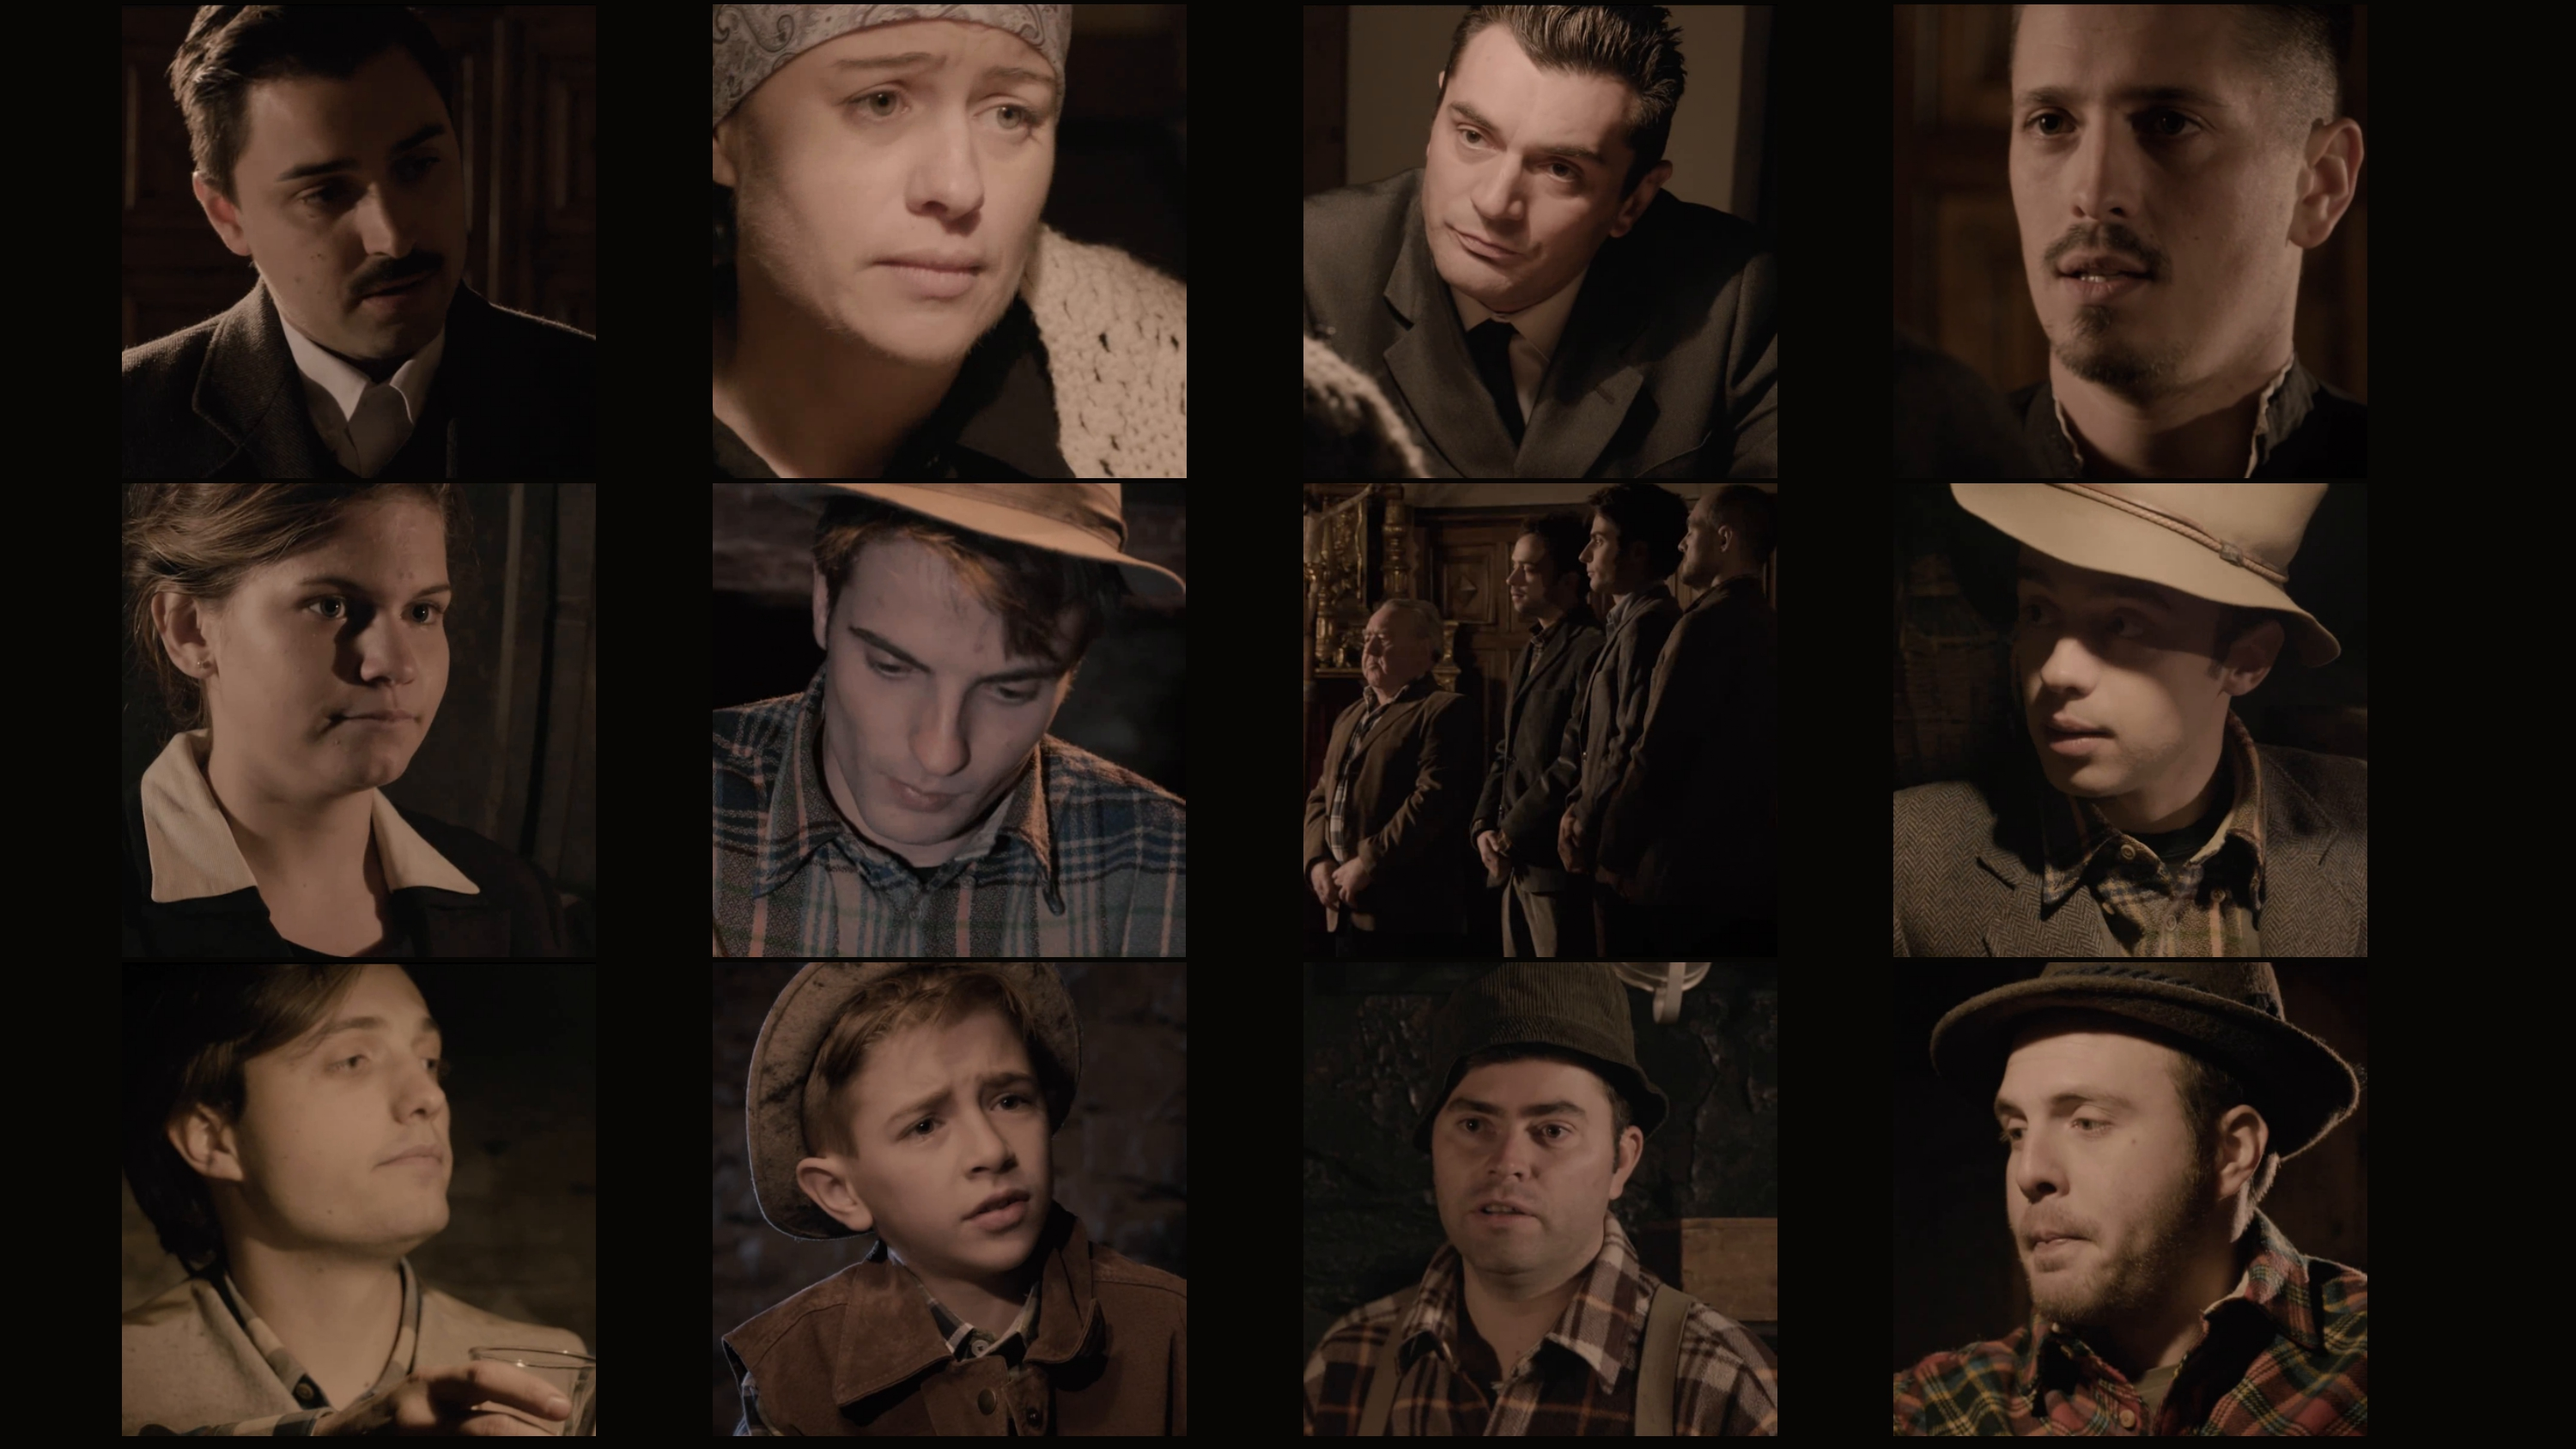
\includegraphics[height=4cm,keepaspectratio]{Foto/2017/gruppo.jpg}
}
\end{figure}
\noindent
\textbf{Dameun}: \textit{Paolo Dall'Ara, Jo\"{e}lle Bollon, Paolo Cima Sander, Marco Ducly.}
\newline
\newline
\textbf{I mentèn}: \textit{Marlène Jorrioz, André Comé, la tsantiì avouì Renzo Bollon, Jordy Bollon,  André Comé é Ronny Borbey, Jordy Bollon.}
\newline
\newline
\textbf{Dézò}: \textit{Richard Cunéaz, Aimé Squinabol, Jo\"{e}l Albaney, Simone Roveyaz.}

\LinkPiese{RECONSTITUTION\\ La vèille di gran dz\^{o}}{https://www.youtube.com/watch?v=A096ZsJ-N0k&t=10s}{.5}

\section*{Eun \textit{court-métrage}?}
Deun l'aout\'on di 2016, l'ie pa eunc\'o cheur que lo Printemps Thé\^atral sarie it\'o organizoù. I mimo ten, le Digourdì l'ayoon resì pe l'Administrach\'on comunale la propozich\'on de réalizé eun courmétradzo avouì eunna équipe de professioniste. L'ie cheur eun projé pa seumplo pe eunna pégna compagnì de téatre sensa espérianse deun lo mondo di \textit{cinéma}. Mi, i mimo ten, l'ie eun projé que l'arie baillà i Digourdì eunna noua voya de recomenchì, aprì eunna dériye pièse, ``N'en pa lo ten", que l'ayè eunna mia tchoué l'entouziasme dedeun la compagnì. 
\\Donque, lo directif l'ayè désidoù de pa partisipé i Printemps Thé\^atral di 2017, deun lo cas que fuche it\'o organizoù\footnote{ \textit{Heuresement} l'è itoù organizoù.}, pe pouèi bouré totte le-z-énerjì deun la produch\'on di premì \textit{court-métrage} di Digourdì.

\section*{Lo souvenir di Seunteucco}
\og N'en voulì counté l'istouére moderne de noutra Quemeua avouì eun langadzo directe, \textit{visuel}, eun proupouzèn i Digourdì eun défì: dzoure leur caletaye é leur espérianse téatrale pe réalizé eun \textit{court-métrage}. Imajin-ì la vèille di premiye-z-éléch\'on tsarvensolentse aprì la Secounda Guerà mondiale, l'a bailla-no la possibilitoù de rappelé tcheu sise que l'an i a queur Tsarvensoù, mimo aprì le-z-àn teuppe di \textit{fascisme}; mi surtoù de commémoré le sinque Père de Tsarvensoù (comme lamo le querì mé!), que l'an portoù la Quemeua i premiye-z-éléch\'on de Tsarvensoù reconstituite.
\\Personellamente, l'è it\'o émouvàn veure comme se pou baillì viya a eun boc\'on d'istouére avouì l'\textit{art cinématographique}. Mimo lo fé que le-z-atteur sayoon de dzouveun-o Tsarvensolèn l'è eun souvenir prèsieu que n'i\ldots pequé, eunsemblo, n'en cougnì, é eun caque magniye viquì, eunna padze eumpourtanta de noutra Communoté.
%Anche il fatto che gli attori fossero tutti giovani e del territorio ha permesso che anche loro venissero a conoscenza di una pagina che ignoravano.
%Personalmente, è stato emozionante veder ricostruire all'interno di un set cinematograrica la storia del nostro comune
%Perché abbiamo voluto raccontare la storia moderna del nostro comune utilizzando un linguaggio immediato e proponendo ai diogurdì una sfida, ossia di cimentarsi nella realizzazione di una pièce teatrale.
%Ripercorre la storia della notte prima delle elezioni, ci ha permesso di ricrodare tutti coloro chehanno sempre avuoto a cuore il nostro comune nonostante gli anni bui della sopressione e soprattutto i cinque,c he amo def padri fondagori, che in prima persona hanno portato il comune alle libere elezioni del 46 continuando per la maggior parte l'impegno nella legislatura successiva.
\fg{}
\newline
\newline
\hspace*{\fill} \textit{Ronny Borbey}

%

\queriaouzitou{
\begin{itemize}
\item[$\bullet$]  \og La vèille di grand dz\^o \fg{} l'è it\'o lo premì \textit{court-métrage} de la compagnì Le Digourdì.\vfill

\item[$\bullet$] \og La vèille di grand dz\^o \fg{} l'è eunc\'o lo débù de Aimé Squinabol deun Le Digourdì comme acteur. L'ie dza pouyà si lo palque deun l'an 2012, mi maque avouì eunna pégna apparich\'on sensa battiye.\vfill

\item[$\bullet$] Renzo, que eunterprète eun tsantre de la parotse, sayè pa qué que sarè itoù reprèi. Jordy l'ayè maque deu-lei que dèijè baillì eunna man pe tramé de moublo.
\end{itemize}
}

\Scenographie
\begin{itemize}
\item[$\bullet$] \'Eillize de \textit{Sainte Colombe} - Tsarvensoù;
\item[$\bullet$] Lèitì di veladzo di Plan - Euntroù;
\item[$\bullet$] \textit{Maison} Bruil d'Euntroù - Crotta avouì 1 tabla, 3 caèye, 1 botéill\'on, 3 vèyo é eunna bocon-où;
\item[$\bullet$] Pailleu avouì 1 banquetta;
\item[$\bullet$] 1 tsaèn avouì de boate;
\item[$\bullet$] \textit{Centre d'études francoprovençales} René Willien - Quezeun-a di-z-àn '40 avouì 1 tabla é 2 caèye. 
\end{itemize}

\setlength{\lengthchar}{3.40cm}

\Character[EMERICO]{}{g}{Emerico Comé, Tsarvensolèn classe 1890, directeur de la tsantiì deun le-z-àn '40, \name{Paolo Dall'Ara}}

\Character[Tsantre I]{}{g}{Tsantre de la parotse de Tsarvensoù, \name{Jordy Bollon}}

\Character[Tsantre II]{}{g}{Tsantre de la parotse de Tsarvensoù, \name{Renzo Bollon}}

\Character[Tsantre III]{}{g}{Tsantre de la parotse de Tsarvensoù, \name{Ronny Borbey}}

\Character[Tsantre IV]{}{g}{Tsantre de la parotse de Tsarvensoù, \name{André Comé}}

\Character[PRIYE]{}{g}{Abbé Hilarion Vection, priye de Tsarvensoù, \name{Marco Ducly}}

\Character[LOUIS]{}{g}{Louis Lucianaz, Tsarvensolèn classe 1901, \name{Jo\"{e}l Albaney}}

\Character[ADELLINE]{}{g}{Adelline Lucianaz, métressa de l'icoula de Tsarvensoù deun le-z-àn '40, \nameF{Marlène Jorrioz}}

\Character[AMÌ DE AIMÉ I]{}{g}{Eun Tsarvensolèn que lame djouì a la moura, \name{Richard Cunéaz}}

\Character[AMÌ DE AIMÉ II]{}{g}{Eun Tsarvensolèn que lame djouì a la moura, \name{Simone Roveyaz}}

\Character[AIMÉ]{}{g}{Aimé Damien Borbey, Tsarvensolèn classe 1897, \name{Jordy Bollon}}

\Character[JOSEPH]{}{g}{Mèinoù tsarvensolèn di-z-àn '40, \name{Aimé Squinabol}}

\Character[JUSTIN]{}{g}{Justin Donzel, Tsarvensolèn classe 1898, \name{André Comé}}

\Character[SABINE]{}{g}{Sabine Lucianaz Savioz, fenna de César Savioz, \nameF{Jo\"{e}lle Bollon}}

\Character[C\'ESAR ]{}{g}{César Savioz, Tsarvensolèn classe 1897,  \name{Paolo Cima Sander}}

\DramPer

\act[RECONSTITUTION\\ La vèille di gran dz\^{o}]

Aprì la Secounda Guèra mondiale, lo 17 di mèis de mi di 1945, lo préfé de Veulla Alessandro Passerin d'Entrèves publiye eunna \textit{circulaire} pe la reconstituch\'on de totte le Quemeue ran\-tchaye pe lo réjime fasiste.

Lo 27 janvieur 1946, 424 Tsarvensolèn é Tsarvensolentse dimandon a la Préfetteua de Veulla la reconstituch\'on de la Quemeua de Tsarvensoù. Lo 30 avrì 1946, lo prof. Federico Chabod, Prézidàn di Conseille de la Val d'Outa, décllare la reconstituch\'on de Tsarvensoù.

Lo 30 joueun 1946, son élì sinque \textit{membre} de la jeunte eun\-tsardjaye de refondé la Quemeua: Aimé Borbey, Emerico Comé, Justin Donzel, Louis Lucianaz é César Savioz.

Lo 23 novembre 1946, vèille di premiye-z-éléch\'on comunale de Tsarvensoù reconstituiya, Aimé, Emerico, Justin, Louis é César viquèison Tsarvensoù comme totte le-z-atre nite, mi avouì lo queur que  boueuche i dzor aprì, lo gran dzor. Eunna nite coloraye avouì salle attivitoù jénuine d'eunna pégna communoté: le proue de la tsantiì, la lèitì, le counte avouì le-z-amì, le traille de la véillà, la chaleur de la fameuille. Eunna nite icllériaye di fouà de la spéranse que brille deun le joueu  queriaou di pégno Joseph. Demàn se recomenche, \textit{démocratiquement}, avouì eun Consèille tsarvensolèn.

\DeriLeRido
\RoleNoms{Sujé é teste}{Le Digourdì,
Chiara Bernardi, Ronny Borbey}
\RoleNoms{Traduch\'on}{Raffaella Lucianaz}
\RoleNoms{Son}{Giovanni Corona, Raffaele D'Anello}
\RoleNoms{Produch\'on ézécutive}{Giulia Di Francescantonio}
\RoleNoms{Produch\'on}{\textit{Ezechiele} 25$:$17}
\RoleNoms{Fotografie é réjì}{Alessandro Stevanon}
%\title{TODZO PI DIGOURDÌ}
\author{Pièse icrita pe Le Digourdì}
\date{Téatro Splendor de Veulla, 10 marse 2018}

\maketitle

\fotocopertina{Foto/2018/gruppo_red.jpg}{Sophie Comé, Ronny Borbey, Francesca Lucianaz, Paolo Cima Sander, Julie Squinabol, Jo\"{e}l Albaney, Michel Comé, Marco Ducly, Stephanie Albaney, Thierry Jorrioz, Simone Roveyaz, Aimé squinabol, Marlène Jorrioz, Paolo Dall'Ara, Richard Cunéaz}{Evi Garbolino, Jo\"{e}lle Bollon, Pierre Savioz, Jordy Bollon, Laurent Chuc, André Comé}{2018}

\LinkPiese{Avanspettaclle, Todzo pi Digourdì}{https://www.youtube.com/watch?v=IaFisR_YuYo&list=PLBofM-NS_eLJUln45l7VH457fGak_Bk5O&index=4, https://www.youtube.com/watch?v=MiAzDgBoOTY}{.45}

\souvenir{La pièse \og Todzo pi Digourdì \fg l'è itaye icrita eugn'occaj\'on di dji-z-àn de la Compagnì. Lo sujé di teste l'è la \textit{biographie ironique} di Digourdì.
Personellamente \og Todzo pi Digourdì\fg resterè todzor deun mon queur, pe bièn de rèizón.

L'è itaye la dériye pièse comme Prézidàn di Digourdì; l'è eunna pièse avouì laquella eugn  itrandjì pou comprendre amod\-do sen que vou deue itre Digourdì, di momàn que lo \textit{fil rouge} de la counta l'è l'esprì comique de totta la compagnì, avouì voya de riye pe fée riye; l'è itoù lo premì cou iaou la Compagnì l'a prooù a tsandjì \textit{style} téatral: \textit{scénographie} redouite i \textit{minimum}, \textit{scène} reprézentaye deun difièn conteste \textit{espace-temps}\footnote{ Eun premì tentatif l'ie itoù fé avouì la pièse \og Matte\ldots sen tcheut matte\fg{} deun lo 2013.}, \textit{mimétisme} é surtoù bièn de \textit{métathéâtre}.}{Jordy Bollon}
\queriaouzitou{
\begin{itemize}
\item[$\bullet$] La grafie di titre de la pièse l'è pa correcte:  \og Todzo\fg{} se devriye icriye \og Todzor\fg{}. Dièn pa lo non di/de la responsablo/a de seutta erreur pe pa provoqué de discuch\'on inutile. Can mimo, va la pèin-a de soulignì pequé n’en desidoù de vardé lo titre trompoù. Pe doe rèiz\'on: premì, pe no rappelé de fé pi attenchón avouì la grafiye di teste que no publièn; secón, di momàn que la pièse counte de fasón \textit{autoironique} sen que vou deu itre Digourdì, eun titre avouì eunna petchouda erreur l'ie bièn reprézentatif di sujé de la pièse mima.\\

\item[$\bullet$] Deun la scène X - La Nite di-z-Oscar, noutro Paolo Cima Sander repette, deun eunna meneutta é demì, nou cou \og can mimo\fg{} é chouì cou \og eumpourtàn\fg{}!

\refstepcounter{videos}
\begin{figure}[H]
\vspace*{-5pt}
\centering
\begin{subfigure}{.75\textwidth}
\centering
\video\hspace*{0.5mm} \textsc{\small Can mimo vs Eumpourtan}\hspace*{0.5mm} \video\\\vspace*{1mm}
    \qrcode[hyperlink, height=0.5in]{https://www.youtube.com/watch?v=tCJzWhbbfCQ}
\end{subfigure}%
\addcontentsline{vds}{section}{Canmimo vs Eumpourtàn}
\end{figure}

\item[$\bullet$] Deun l'avanspettaclle, le dou prézentateur son réel\-la\-men\-te lo Seunteucco é lo Vise Seunteucco de la Quemeua de Tsarvensoù. 
\end{itemize}
}

\Scenographie
\begin{itemize}
\item[$\bullet$] 1 poltronna moderna;
\item[$\bullet$] 1 chofà;
\item[$\bullet$] 1 peuccapoussa \aspirapolvere\ \textit{automatique};
\item[$\bullet$] 1 \textit{hoverboard};
\item[$\bullet$] 1 \textit{album} di foto;
\item[$\bullet$] 1 ban de eunna cantin-a iaou aprésté lo bèye pe le clliàn;
\item[$\bullet$] 2 pégne table, comme salle di cantin-e ;
\item[$\bullet$] 15 caèye que se pouon pléì, comodde pe itre tramaye eun pocca ten;
\item[$\bullet$] 1 volàn di poulmeun;
\item[$\bullet$] 1 \textit{pupitre};
\item[$\bullet$] 1 busta;
\item[$\bullet$]1 Oscar.
\end{itemize}

\setlength{\lengthchar}{3.5cm}

\Character[LAURENT]{LAURENT}{Laurent}{Premì prézentateur, lo Vise Seunteucco de Tsarvensoù, \name{Laurent Chuc}}

\Character[RONNY]{RONNY}{Ronny}{Sec\'on prézentateur, lo Seunteucco de Tsarvensoù, \name{Ronny Borbey}}

\Character[MAGÀN]{MAGÀN}{Magan}{Magàn Sophie \viille, sa eumpléì amoddo lo téléfonne é la tecnolojì, \nameF{Sophie Comé}}

\Character[PAGÀN]{PAGÀN}{Pagan}{Pagàn Paul \viou, euncó llou bièn tecnolojique, \name{Paolo Dall'Ara}}

\Character[NEVAOU]{NEVAOU}{Nevaou}{Nevaou de pagàn Paul é magàn Sophie, \name{Aimé Squinabol}}

\Character[NEVAOUZA]{NEVAOUZA}{Nevaousa}{Nevaouza de pagàn Paul é magàn Sophie, \nameF{Julie Squinabol}}

\Character[SERVENTA]{SERVENTA}{Serventa}{Serventa d'eunna cantin-a de Tsarvensoù,  \nameF{Stéphanie Albaney}}

\Character[FRANCESCA]{FRANCESCA}{Francesca}{La vrèya Francesca Lucianaz di Chef-Lieu, \nameF{Marlène Jorrioz}}

\Character[PIERRE]{PIERRE}{Pierre}{Lo vrèi Pierre Savioz di Tsatì, \name{Pierre Savioz}}

\Character[JO\"{E}LLE]{JO\"{E}LLE}{Joelle}{La vrèya Jo\"{e}lle Bollon di Chef-Lieu, \nameF{Jo\"{e}lle Bollon}}

\Character[JO\"{E}L]{JO\"{E}L}{Joel}{Lo vrèi Jo\"{e}l Albaney d'Ampaillan, \name{Jo\"{e}l Albaney}}

\Character[VÉTCHOT]{VÉTCHOT}{Vetchot}{Eun vétchot \viou\ di péì, tchica boutro, \name{Richard Cunéaz}}

\Character[CIMA]{CIMA}{Cima}{Lo vrèi Paolo Cima Sander de Feleunna, \name{Paolo Cima Sander}}

\Character[MARCO]{MARCO}{Marco}{Lo vrèi Marco Ducly de Feleunna, \name{Marco Ducly}}

\Character[SIMONE]{SIMONE}{Simone}{Lo vrèi Simone Roveyaz di Pon-Sià, \name{Simone Roveyaz}}

\Character[ÉLEVEUR]{ÉLEVEUR}{Spectateur}{\'Eleveur tsarvensolèn, \name{Thierry Jorrioz}}

\Character[MAMMA]{MAMMA}{Mamma}{Eunna mamma d'eun atteur di Digourdì, \nameF{Stéphanie Albaney}}

\Character[TSACHAOU I]{TSACHAOU I}{TsachaouI}{Eun tsachaou de Tsarvensoù, \name{Jordy Bollon}}

\Character[TSACHAOU II]{TSACHAOU II}{TsachaouII}{Eungn atro tsachaou de Tsarvensoù, \name{André Comé}}

\Character[FOTOGRAFE]{FOTOGRAFE}{Fotografe}{Vioù fotografe di Printemps Thé\^atral, an mia trambelìn, \name{Thierry Jorrioz}}

\Character[CHAUFFEUR]{CHAUFFEUR}{Chauffeur}{\textit{Chauffeur} di poulmeun pe la chortia annuella di Digourdì, \name{André Comé}}

\Character[JORDY]{JORDY}{Jordy}{Lo vrèi Jordy Bollon di Chef-Lieu, \name{Jordy Bollon}}

\Character[THIERRY]{THIERRY}{Thierry}{Lo vrèi Thierry Jorrioz di Chef-Lieu, \name{Thierry Jorrioz}}

\Character[STEPHANIE]{STEPHANIE}{Stephanie}{La vrèya Stephanie Albaney d'Ampaillan, \nameF{Stéphanie Albaney}}

\Character[CONDUCTEUR]{CONDUCTEUR}{Conducteur}{Conducteur télévizif de la nite di-z-Oscar, \name{Richard Cunéaz}}

\Character[ASSISTANTA]{ASSISTANTA}{Valletta}{Assistanta di conducteur télévizif, \nameF{Stéphanie Albaney}}

\Character[]{LE DOU NEVAOU}{Ledou}{\quad}

\Character[]{TCHEUTTE}{Tcheutte}{\quad}

\DramPer

\act[\avanSpect\ Avanspettaclle   \avanSpect]

\StageDir{\hspace*{2.5em}Lemie \lemieSi.}

\StageDir{\hspace*{2.5em}Laurent l'è si \textit{proscenium} que avèitse lo pebleuque.}

\begin{drama}

\Laurentspeaks Bonsouar é bienvenù a tcheutte a seutta souaré di Printemps Thé$\hat{a}$tral avouì le Digourdì de Tsarvensoù. Me semble ieur can no sen acapó lo premì cou comme compagnì é n'en désidoù de beté si le Digourdì. Dèi si dzor lé n'en fé tan de souaré é de chortie, todzor eun vardèn lo mimo esprì, la mima voya de riye é de fé riye. Donque, eugn'occajón de noutro anniverséo, n’ayòn désidó de pourté inque si lo palque eun momàn bièn tipique, é sourtoù bièn téatral, de sen que l'iye la viya valdoténa: lo Consèille réjonal. Mi aprì no no sen deu: mi le dzi veugnon sé pe riye ou pe plaoué? Pe riye! É ad\'on no no sen deu: na, na, na! L'è vrèi que lo téatro é la poleteucca son bièn gropoù; bièn de cou te comprèn pa qui fé la poleteucca é qui fé lo téatro. Mi i mimo ten, euncó no Digourdì pouèn pa tan cretequì la poleteucca; euncó no n'en noutro pégno euntsardzo eun poleteucca. La Joueunte comunalla de Tsarvensoù l'è compozaye pe cattro Digourdì si sinque! N'en la majoranse! \'E l'unique que l'è pa eun Digourdì, lo seul que l'a jamì resitó desì si palque (é de so dèi se baillì lagne)\ldots l'è noutro Seunteucco! Seunteucco, que comme tcheu le vrèi politisièn, l'è vin-ì eun salle de téatro, l'a saroù la man a tcheutte, l'è fé-se vére, l'a fé de grou sourì\ldots é ara iaou l'è aloù? L'è aloù ià! Mi l'a pa comprèi que sise que l'an resitoù devàn sayòn sise de Brutchón! Pa de Tsarvensoù! Mi se pou beté Seunteucco eun que prèdze gnenca noutro patoué? Mé ara dimando a tcheu vo\ldots mi se pou voté eun Seunteucco que\ldots

\StageDir{Ronny Borbey, Seunteucco de Tsarvensoù, entre eun \textit{scène}.}

\Ronnyspeaks Laurent! Avèitsa que\ldots se te vou conten-ì a fé lo Vise Seunteucco tanque lo 2020\ldots fé attench\'on a sen que te di!

\Laurentspeaks Mi té de iaou t’i entroù?

\Ronnyspeaks N'a pa d'eumpourtanse de iaou si entroù! Te semble lo case  de diye de bague di janre?

\Laurentspeaks T'a rèiz\'on\ldots

\Ronnyspeaks Ouè que n'i rèiz\'on!

\Laurentspeaks Mi ara que sanse l'a deusqueté douàn a totte seutte personne?

\Ronnyspeaks Na l'a pa de sanse. Surtoù pequé fa planté-la lé de deusqueté comme eun Consèille réjonal. Se comprèn jamì ren: eun chor de la majoranse, l'atro entre deun la majoranse, aprì l'atro euncoa chor de la minoranse, si de douàn entre eun minoranse\ldots se comprèn pamì ren! Mi prao, fa avèitchì i futur, djeusto?

\Laurentspeaks Ouè! Mé diyo: pequé profitèn pa de totte seutte personne pe comenché a icriye lo programme di prochèn-e-z-éléchón?

\Ronnyspeaks Djeusto! Mi te diyo eungn atra baga: fièn comme fan le Grilleun!

\Laurentspeaks Ah ouè le sinque-z-itèile!

\Ronnyspeaks Djeusto! Leu senque fan? Demandon i dzi se son d’acor, beutton eun votach\'on, fan le \textit{parlamentarie}. Comme lo PD que fé le \textit{primarie}.

\Laurentspeaks \ldots é ad\'on no senque fièn?

\Ronnyspeaks Fièn le tsarvensarie! Demandèn i dzi se son d’acor.

\Laurentspeaks Va bièn, comenchèn!

\Ronnyspeaks Té pensa a doe bague: i spor é a l'imondicha\ldots

\Laurentspeaks Ah l'imondicha! N'i dza deu-lo eun Consèille, a la majoranse é a la minoranse que l'imondicha l'è pa eunna compétanse de la Quemeua, mi de l'Unité!

\Ronnyspeaks \ldots é ad\'on pensa i tourisme. Va bièn?

\Laurentspeaks Ouè; é té pensa a la queulteua é i travó poubleucco.

\Ronnyspeaks Va bièn. Ad\'on atacca té!

\Laurentspeaks Atacco\ldots ad\'on\ldots spor\ldots n'i eunna idé dèi can sayò ate pouèi \direct{avouì la man moutre l'atchaou}, dièn dèi can sayò pégno: eunna grousa manifestach\'on, bièn eumpourtanta\ldots

\Ronnyspeaks \ldots pa la Becca!

\Laurentspeaks Na bièn pi grou! Vouillo pourté a Tsarvensoù le Jeux Olympiques!

\Ronnyspeaks A Tsarvensoù? Mi se pou pa! N'en lo caro pe totte le streutteue?

\Laurentspeaks Ouè! Fé-me esplequì! N'en tot: ba pe la plan-a, protso de la grandze, protso di mitcho de Franco Lucianaz fièn eunna grousa streutteua pe saouté avouì le-z-esquì; aprì fièn lo restoràn iaou betèn traillì tcheu sise de Valpettaz!

\Ronnyspeaks Ah pouèi areuvvon le vouése de Valpettaz!

\Laurentspeaks Ouè,  30 ou 40 vouése! Aprì lo fondo\ldots lo fièn si a Tsan-Plan; betèn eunna grousa cabouetta pe le beillette, eunna dzenta cantin-a iaou fièn traillì sise di Combes é di Tsatì!

\Ronnyspeaks \ldots é lé d'atre vouése!

\Laurentspeaks Son 200 vouése! Aprì lo bob: lo fièn partì si i rascar de Combatechiye\ldots

\Ronnyspeaks Mi gneun reste si pe de lé! Queunte vouése prégnèn?

\Laurentspeaks Ouè mi la feun de la pista di bob la fièn devàn lo mitcho de Diego Bollon! Countèn Diego countèn le Bollon, countèn le Bollon countèn Sen-Sal\'o !

\Ronnyspeaks Le Bollon son tan é no voton tcheutte!

\Laurentspeaks Mi pe gagnì le-z-éléch\'on fa euncó avèitchì la partia basa. Lé fièn eunna grousa \textit{patinoire} é la fièn jéré a Franco Lombardo!

\Ronnyspeaks Lé son 300 vouése! Sen a poste! 

\Laurentspeaks Garantì,  300 vouése!

\Ronnyspeaks Me plé!

\Laurentspeaks Mé avouì lo spor si a poste. Ara té pensa a la queulteua.

\Ronnyspeaks Acouta-mé: no n'en cherdì le Digourdì pe fé lo \textit{court-métrage} si la Reconstituch\'on de la Quemeua; le DVD l'an i eun gran sucsé! Ad\'on senque fièn? Pourtèn a Tsarvensoù lo festival di \textit{cinéma} de Cannes é de Venize! Imajina-té le journal:\fg Festival di \textit{cinéma} de Tsarvensoù\og{}!

\Laurentspeaks Wow!

\Ronnyspeaks Imajina le \textit{star} que se fan le \textit{selfie} si la promenade!

\Laurentspeaks Ah ah ah! Mi iaou sarie noutra promenade?

\Ronnyspeaks Mi n'en euncó no la promenade: lo tsemeun de Veulla! Imajina-té le \textit{star} que van si é ba pe lo tsemeun de Veulla!

\Laurentspeaks Si é ba, ba é si!

\Ronnyspeaks Se fan le \textit{selfie} é aprì fièn finque la directe avouì Barbara d'Urso, avouì lo programme \og Iproù 5\fg{}!

\Laurentspeaks Pa mal!

\Ronnyspeaks Pouèi acapèn euncó le vouése di fenne que steurion!

\Laurentspeaks Ouè, djeusto, salle son de tsaplette.

\Ronnyspeaks Ara té pensa i tourisme\ldots

\Laurentspeaks Tourisme\ldots sel\'on mé fa fé eunna téléférique que partèi de Plase Chanoux, areuvve si i Chef-Lieu, aprì pase euncó protso sen di Borbey, conteneuvve tanque si i val\'on de Combouì é a la feun s'arite si i refuje Arbolle.

\Ronnyspeaks Pa mal!

\Laurentspeaks Ouè, pouèi le portèn tcheutte si eugn Arbolle, bèyon lo cafì pi bon i mondo (lo Cafì Ollietti), mi surtoù\ldots payon! Le fièn paì la tasse de \textit{soggiorno}!

\Ronnyspeaks Pequé sise no voton pa, pequé iton pa a Tsarvensoù.

\Laurentspeaks Ouè, no voton pa mi payon! Baillon de sou a la Quemeua, la Quemeua baille de sou i sitouayèn, le sitouayèn son contèn é le sitouayèn contèn no voton!

\Ronnyspeaks Sen a poste.

\Laurentspeaks Ouè! Mi pe gagnì fa todzor prendre eun considérach\'on eunna baga: le trav\'o poubleucco. Si so, queutto la paolla a té.

\Ronnyspeaks Donque fé-me pensì\ldots n'i pensoù. Ad\'on té te cougnì amoddo la Becca, mi te feré pi eugn'atra manifestach\'on: Veulla - Tsarvensoù - Mont-Emilius, pouèi te va euncó pi si!

\Laurentspeaks Na si pa d'acor!

\Ronnyspeaks Atèn que t'euspleucco. Te sa senque fièn de la poueunte de la Becca?  La copèn!

\Laurentspeaks Naaa! Comèn copé la Becca?

\Ronnyspeaks Ouè!

\Laurentspeaks \direct{Dispéoù} Na! Copé la Becca! Na votade pa! Na!

\Ronnyspeaks Acoutta! Copèn la Becca pequé pouèi portèn lo solèi a Roulaz é prégnèn totte le vouése de Roulaz; no vote finque Anselmino que la jamì votou-no! Portèn aprì lo solèi a Feleunna! Counta véo de vouése a Feleunna!

\Laurentspeaks Mondjemé! Eunna sentèin-a!

\Ronnyspeaks \ldots é pourtèn finque lo solèi a Plan-Feleunna! Counta le vouése\ldots

\Laurentspeaks N'i pa praou de dèi! Va bièn, si caze d'acor; mi la Becca iaou la betèn?

\Ronnyspeaks N'i pensoù euncó a so: lo pro de la grandze de Plan-Feleunna. Atsetèn lo pro (le tsanéno l'an fata de sou pe se paì la \textit{badante}), plachèn la Becca é fièn Charvland, lo Gardaland de Tsarvensoù! L'è pa eunna dzenta idoù?

\Laurentspeaks L'è eunna idoù euncrouayabla! A Charvland lèi betèn a traillì sise de la Giradaz, sise d'Ampaillan, sise di Pont-Suaz. Aprì totte le-z-attivitoù di Pon travaillon de pi é se travaillon no voton!

\Ronnyspeaks Eh ouè!

\Laurentspeaks Mé diyo que sel\'on mé n'a la caèya pe 30 an!

\Ronnyspeaks Cheur\ldots mi n'en deu devàn que fa demandé i dzi se son d'acor: fa fé le Tsarvensarie.

\Laurentspeaks Mi n'a pa fata avouì si programme!

\Ronnyspeaks Fien-leu pequé no sen comme le Grilleun démocratique\ldots é propozèn eun programme fattiblo!

\Laurentspeaks No sen de Valdotèn, sen pa sé pe counté de counte foule! Sen que dièn lo fièn!

\Ronnyspeaks Se pou fiye! Ad\'on mé beutto eun votach\'on: countréo?

\StageDir{Ronny é Laurent avèitson lo poubleucco.}

\Laurentspeaks Me semble gneun\ldots té avèitsa si, que mé avèitso ba.

\Ronnyspeaks Gneun! Amoddo! Ara demando: favorable?

\StageDir{Ronny é Laurent avèitson tourna lo poubleucco.}

\Laurentspeaks Avèitsa qui la votou-no! La votou-no finque Siro Viérin! Mi demàn nèi!

\Ronnyspeaks N'en l'unanimitoù. Saren-no la man pe la fotografie avouì le journaliste\ldots

\StageDir{Ronny é Laurent se saron la man é sourion pe se fé fé eunna foto. Aprì chorton.}

\Laurentspeaks Ah na!

\StageDir{Ronny é Laurent tornon i mentèn di palque.}

\Ronnyspeaks Na sen oublia-no di Digourdì!

\Laurentspeaks Donque vo quetèn avouì lo spettaclle di Digourdì icrì eun occaj\'on di djijimo anniverséo de la compagnì! A vo\ldots

\Ronnyspeaks Todzor pi\ldots

\Tcheuttespeaks \ldots Digourdì!

\act[Acte I]

\ridoiver

\scene[-- L'\textit{album} di Digourdì]

\StageDir{Lemie \lemieSi\ a drèite di palque, iaou acapèn eun chofà é magàn protso d'eunna poltronna.\\ \Fv{Tsarvensoù, 4 janvieu 2050}
}

\Maganspeaks \direct{Eun se achouatèn si la poltronna} Oh\ldots si belle lagnaye! Ara m'achouatto eun momàn. Ah na! Me fa euncó poulité lé pe tèra. Ah! Mi n'i la soluch\'on! Lola!

\StageDir{Eun peuccapoussa \textit{automatique} chor foua di chofà é poulite sel\'on sen que comande Magàn.}

\Maganspeaks Oh saye! Voualà, poulita an mia pi a drèite\ldots pi a gotse\ldots Stop! Ara tourna i teun poste, a coutcha!

\StageDir{Lo peuccapoussa se bloque.}

\Maganspeaks Seutte baradziye, martson pa. Le beutto a poste mé.

\StageDir{Magàn se levve é catse lo peuccapoussa dézò lo chofà. Aprì s'achouatte tourna si la poltronna é teurie foua lo portable.}

\Maganspeaks\direct{Eun lièn} Véyèn sen que conte-tì lo moundo oueu\ldots

\StageDir{Entre pagàn avouì l’\textit{hoverboard}.}

\Paganspeaks Sophie! Si arevoù!

\Maganspeaks L'iye l’aoua bon!

\Paganspeaks \direct{Eun se boudzèn avouì l’\textit{hoverboard}} N'i fé eunna dzenta promin-ada oueu\ldots avouì la dzenta mezeucca de l’Orage n'i fé belle dou \textit{kilomètre}!

\Maganspeaks \ldots é t'i nienca tsizì! T'i fran eun gamba!

\StageDir{Pagàn fé dou tor si lo poste é aprì bèiche ba de l’\textit{hoverboard}.}

\Paganspeaks \`Eitsa que mé si eungn esper de seutte machine! Pa comme té, todzor dérì a si portablo é a Facebook é iPhone!

\Maganspeaks \`Eitsa que mé oueu n'i dza to fé, n'i dza to poulit\'o !

\StageDir{Pagàn s'achouatte si lo chofà.}

\Paganspeaks Ouè, poulit\'o avouì salle machine que t'a pe lo mitcho\ldots que nen si mé sen que te combeun-e pe lo mitcho! \direct{Eun terièn foua lo portablo} Ara fé-me lie lo journal.

\Paganspeaks \`Eitsa Sophie! Amélie Viérin noua Prézidante de la Réj\'on\ldots eh, Sophie, dza lo pappa Laurent l'ayè fé lo Prézidàn 30 an fé!

\Maganspeaks \ldots é lo pappagràn l'ayè fé-lo dza i seun ten!

\Paganspeaks Ouè, que dzen veure comèn le mitchì se tramandon, l'è dzen so!

\Maganspeaks T'a fran rèiz\'on!

\StageDir{Le dou nevaou entron eun galopèn avouì eun man eun grou album di fotografie. S'achouatton protso de pagàn.}

\Ledouspeaks Pagàn, pagàn! Senque l'è si grou livro?

\Nevaousaspeaks L'è icrì: \og Le Digourdì! \fg{}

\Paganspeaks Aimé, Julie! Mi iaou v'ouèide acapoù so?  

\StageDir{Pagàn pren lo livro eun man é lèi souffle desì pe lèi gavé ià la poussa\footnote{ Commé éffé spésial n'en betoù bièn de \textit{borotalco} deun l'\textit{album}, pe fé vère la poussa can pagàn lèi soufflè desì.}.}

\Paganspeaks\direct{Eton-où \ouaou} Mi sit\ldots \direct{avèitse Magàn} té t'a catcha-lo!

\Maganspeaks Na!

\Paganspeaks Si l'è lo livro avouì totte le foto di Digourdì! La pi renoumaye compagnì de téatro de la Val d’Ousta!

\Nevaouspeaks Mi Digourdì qui?!

\Paganspeaks Deh Aimé! Pourta de reuspé pe Le Digourdì! Le Digourdì l'an port\'o lo nom de Tsarvensoù ià pe to lo moundo!

\Nevaousaspeaks Ah ouè? Comèn l'arian fé? Ara éziston-tì eunc\'o ? Can son nèisì?

\Paganspeaks\direct{Bièn fier \tipoconocchiali} Ad\'on\ldots vegnade seu\ldots

\StageDir{Pagàn fé de caro si lo chofà i dou nevaou. Le nevaou s'achouatton.}

\Paganspeaks \ldots ara vo fiyo la conta\ldots l'iye l'an 2000 é\ldots ouette é\ldots

\StageDir{Teuppe \lemieBa\ si la drèite di palque. Lemie \lemieSi\ a gotse é i mentèn di palque.}

\scene[-- La nésanse di Digourdì]

\StageDir{Eun \textit{scène} n'at eun banc\'on é doe pégne table avouì eun per de caèye. N'a la serventa que poulite lo banc\'on é eun vétchot achouatoù a gotse que li lo journal pe son contcho.\\ Entron deun la cantin-a  Jo\"{e}l, Jo\"{e}lle, Pierre é Francesca.}

\Francescaspeaks\direct{A la serventa} Bondzor! T'a eunna plase pe cattro?

\Serventaspeaks Ouè, salla tabla \direct{eun moutrèn la tabla a drèite} va-tì amoddo?

\Francescaspeaks Ouè.

\StageDir{Le cattro-z-amì s'achouatton.}

\Serventaspeaks Sade dza senque bèye?

\Pierrespeaks Féo mé pe tcheutte, fièn cattro bire!

\Francescaspeaks  Na, pe mé te me fé eun ju de frouì i marteun sèque!

\Joellespeaks \ldots é pe mé i-z-ambrocalle!

\Joelspeaks\direct{Eun rièn} I marteun sèque, i-z-ambrocalle! Desandro bèyavade pa tan de ju de frouì\ldots ou mioù: ambrocalle é marteun sèque ouè, mi l'ian dedeun l'éve de viya!

\StageDir{Pierre ri eunsemblo a Jo\"{e}l.}

\Francescaspeaks Euh Jo\"{e}l Albaney! Fa-tì te rapélé que n'i portó té é llou \direct{eun moutrèn Pierre} i mitcho? \'E pe terì si sitta tanque si la Basteuille n'en finque rechà Viro!

\Vetchotspeaks Ouè! Mé alao si i fèye é sise se retèriaon!

\Pierrespeaks\direct{I vétchot} Conteneuvva a lie lo journal! Euncó té can t'ie dzoueun-o t'a fé de fite!

\Vetchotspeaks Penso beun! Mi l'an jamì pourto-me i mitcho le femalle! Todzor arrevó i mitcho avouì l’ape; é pe to diye, i ten de mé le femalle servichaoun pe d’atro!

\Joelspeaks Mi soplé! Li lo journal!

\StageDir{La serventa pourte lo bèye pe le-z-amì.}

\Serventaspeaks Ah ouè \ldots me fiade fran riye: acouté vo me semble de vère lo Charaban!

\StageDir{Silanse. Le cattro-z-amì penson.}

\Joellespeaks Ah lo Charaban\ldots sarie pa mal beté si eunna compagnì de téatro a Tsarvensoù!

\Joelspeaks Pierre! Pourian beté si eunna compagnì de téatro!
 
\Pierrespeaks Pequé pa? Pa mal comme idoù. 

\Joelspeaks\direct{Todzor a Pierre} N'arian djeusto fata de fenne!

\Pierrespeaks Eh ouè sen maque mé é té!

\StageDir{Le dou penson eun momàn dimèn que Jo\"{e}lle é Marlène comenchon a se amalechì pe pa itre considéraye.}

\Pierrespeaks\direct{A la serventa} Squeuza! Té te prèdze beun tchica patoué\ldots

\Serventaspeaks  Pa pi tan\ldots

\Joelspeaks Na mi te lo prèdze bièn! Amoddo!

\Pierrespeaks \ldots é sen a trèi! 

\Joelspeaks Mi n'a pa praou!

\Pierrespeaks\direct{I vetchot} A propoù, té que le femalle te le-z-eumpléyae pe d'atro\ldots

\Vetchotspeaks  Senque?

\Pierrespeaks\direct{I vetchot} Té que t'i plen de femalle, te sarie no deu se n'a de fenne que pouon itre euntéressaye a fé téatro?

\Vetchotspeaks  Argh! Que counte foule, n'i pa lo ten, n'i d’atro pe la tita. Aprì vo senque vouillade fiye? V'ouite cattro rabadàn nèisì ieur, senque nen sade vo de téatro? Soplé!
 
\Joelspeaks  Rappella-té que no dzouin-o fièn sen que n'en voya se n'en la pach\'on! \direct{A Pierre} Mé é té sen prest, n'arian fran voya de comenchì!

\Francescaspeaks Can mimo v'ouite fran pa seumpateucco! Lèi sen mé é Jo\"{e}lle! 

\Pierrespeaks  Mi ouè, té é Jo\"{e}lle! Djeusto, Jo\"{e}lle! Pe case te cougnì pa caque feuille que l'a voya de fé téatro?
 
\Joellespeaks \direct{Malechaye \malechaa} Mi fé-té feun! Mé é Francesca pouèn pa resité avouì vo?
  
\Joelspeaks Say\'on eun tren de squersé!

\Pierrespeaks L'iye pe riye.

\Francescaspeaks\direct{Ironique} Que riye!
\Joellespeaks\direct{Offenchaye} Fran seumpateucco! 

\Pierrespeaks Ad\'on fiade-mé fiye le contcho. \direct{Counte le-z-atteur  de la compagnì} Eun, dou, trèi, cattro é sinque avouì la serventa\ldots pe fé eunna compagnì no manque euncó caqueun.

\Joelspeaks Sen pocca pe ara\ldots

\Pierrespeaks  Ah! L'è vin-i-me eunna idoù! Le premì trèi que entron eun cantin-a le térièn dedeun!

\Joelspeaks Na Pierre n'i pouiye! Avèitsa que reusquèn!

\Pierrespeaks Mi ouè! Sen que capite, capite! A Tsarvensoù sen tcheut amoddo!

\Joelspeaks Na, na, na! \direct{Ver le feuille} Vo v'ouite chiye?

\Joellespeaks Si pa, prouèn.

\Pierrespeaks\direct{A tcheutte} Vo fiade de mé?

\Francescaspeaks Renque pe si cou.

\Joelspeaks Prouèn!

\StageDir{Entre Cima. Le cattro-z-amì se beutton le man pe le pèi.}

\Cimaspeaks \direct{Ver la serventa avouì pach\'on} Bonsouar! Tot amoddo? Te me fé eun dzén-epì tsa? Mi tsa! Maque comme t'i boun-a té a lo fiye \malisieu .

\Serventaspeaks Ouè va bièn.

\Francescaspeaks  Ouè mi sitte l'è de Feleunna é sa gnenca lo patoué!

\Cimaspeaks Feleunna? Feleunna! Mi té can te di Feleunna te di Paolo Cima Sander! Mi gars\'on, chourtade eunna mia de sise \textit{schemi}! Chortade de Tsarvensoù, bèichade ba de salla montagne, ivrade le joueu, végnade avouì no que n’en lo solèi to l’an!

\Joellespeaks\direct{Eun rièn} Na, na\ldots sitte l'è tro rabadàn, l'è eun de no!

\Cimaspeaks Rabadàn? Jo\"{e}llina, mé que n'i pasoù totta la viya a te prédjì, mi reusta quèya\ldots can mimo\ldots

\Pierrespeaks\direct{I seun-z-amì} Vo dimando squiza mi si cheur que le prochèn dou\ldots

\Joelspeaks Na Pierre! Mé n'i tourna  pouiye!

\StageDir{Entron Simone é Marco eun rièn é squersèn. Pierre l'è dispéoù.}

\Joelspeaks\direct{Eun rièn pe pa plaoué} Ah ébeun! L'è pa pi que t'i aloù eun meillorèn!

\Marcospeaks\direct{A Simone} \ldots é desando nite iaou t'i sparì?

\Simonespeaks Ouè Marco, n’ayoù mioù a fiye que itì avouì vo!

\Marcospeaks  Ouè va bièn mi t'a quetou-me a pià a l’Inside \malecha !

\Simonespeaks Veullanoua-Tsarvensoù a pià l'è pa que te lèi beutte tan\ldots

\Marcospeaks Ouè doe meneutte!

\Serventaspeaks Senque béyade?

\Simonespeaks Beutta maque doe bire.

\Pierrespeaks\direct{Ver lo banc\'on} Marco, Simone! Vo laméria fé téatro avouì no?

\Marcospeaks Acoutta mi de feuille nen v'ouèide?

\Joelspeaks Plen pèi!

\Simonespeaks Eunna baga eumpourtanta\ldots de chortie foua Val d'Ousta nen fièn?

\Pierrespeaks Ouè cheur! Tcheu le mèis!

\Marcospeaks Pe mé se pou fiye!

\Pierrespeaks Ad\'on gars\'on, vegnade tcheu seuilla!

\StageDir{Tcheutte se plachon a l'entor de la tabla avouì lo vèyo levoù.}

\Joelspeaks Fièn eun santé a la noua Compagnì de Tsarvensoù!

\Tcheuttespeaks Santé!

\StageDir{Teuppe \lemieBa\ a gotse é i mentèn di palque.}

\StageDir{Lemie \lemieSi\ a drèite di palque.}

\scene[-- Pe to lo moundo \moundo!]

\Paganspeaks Véo d'émoch\'on; 4son dza belle pasoù 40 an!

\Nevaouspeaks\direct{Eunna mia tro savèn} Seutta l'iye pa eunna compagnì de téatre! V'ouyavade eunna compagnì de la crotta!

\Paganspeaks Grama lenva que t'a té!  Pourta reuspé pe le Digourdì! Totsa-meu pa le Digourdì!

\Nevaousaspeaks Squeza-mé pagàn, poui-dze te dimandé eunna baga? Péqué lo nom Digourdì? 

\Paganspeaks\direct{Fier de seutta dimanda} Ah!  Seutta l'è eunna dzenta counta: ad\'on, eun dzor\ldots \direct{comenche a borboté, vague} dou de no son partì ià pe eun mariadzo; aprì can son tournoù i mitcho l'iye tar é l'ay\'on fata de pantchì d'éve\ldots se son betoù protso d'eun meur, mi l'è chortia la mamma de eun de sise dou\ldots la mamma l'a vouaillà : \og Deh! Me raccomando\ldots fiade pa tro le Digourdì! \fg{} . Voualà! De si momàn la Compagnì l'ayè son nom!

\Nevaouspeaks Ouè mi pagàn, se sitte l'è lo nom, vouillo pa imajin-ì le pièse que v'ouèide fé!

\Paganspeaks Aimé! Pourta de reuspé pe le Digourdì é rappella-té que le Digourdì l'an pourtoù lo nom de Tsarvensoù ià pe to lo moundo!

\StageDir{Pagàn se levve.}

\Paganspeaks Té pensa que can n'en fé la premiye pièse,  n’ayè plen de dzi, n’ayè de machine tanque i mentèn de Veulla, n'ayè finque de pompì volontéo de Cogne é Perloz, n’ayè 600 volontéo de totta la Val d'Ousta que l'an édja-no pe fé la premiye! Tourno diye: la premiye!

\Ledouspeaks \direct{Sourprì \ouaou} Pe la premiye 600 volontéo? 

\Maganspeaks\direct{Eun se levèn} Mi senque te counte? \direct{Eun prégnèn l’album é eun s'achouatèn} Acoutade mèinoù, de sen que counte pagàn coppade la mèitchà, vardade eun car é tsapotade euncó eunna mia! Vegnade seuilla  que vo counto mé\ldots

\StageDir{Teuppe \lemieBa\ a drèite di palque.}

\StageDir{Lemie \lemieSi\ a gotse é i mentèn di palque.}

\scene[-- Catro tsatte \gatto\ \gatto\ \gatto\ \gatto]

\StageDir{Si lo palque n'a 15 caèye plachaye si trèi feulle. Eun vétchot é eun éleveur bièn annouiyà son achouatoù si la secounda feulla.}

\StageDir{Eunna mamma entre to de coursa.}

\Mammaspeaks\direct{I vétchot, avouì lo flo queur} Squizade-mé! L'è-tì dza comenchà? 

\Spectateurspeaks Comme tcheu le demicro ataque a ouette é demì!

\Vetchotspeaks  N'a pa de prisa!

\Mammaspeaks Amoddo! Mé ara dèyo vardé eun per de plase pe de paèn.

\StageDir{La mamma comenche a se dizarbeillì pe vardé la plase i seun paèn. Se gave lo palt\'o, eunna maille, eunna botta é le plache si le caèye.}

\Mammaspeaks So pe tanta Filoméne, la siaou, lo botcha\ldots é l'onclle Gene! \direct{Eun gavèn ià eunna caèya é eun se gavèn eunna botta} Pe llou  que areuvve avouì la caèya avouì le raoue queutto eunna botta! 

\StageDir{La mamma finalemàn s'achouatte si la premì  feulla, totta émochon-aye. I contréo, lo vétchot é l'allévateur avèitson torse la mamma.\\ Silanse.}

\Mammaspeaks  Bon mancon seun meneutte! Spéèn que arrevisan tcheutte!

\StageDir{Silanse. Entron dou tsachaou. Eun de leur seuble eunna tsans\'on.}

\TsachaouIspeaks\direct{Eun quetèn  de seblé} N'i la fèi que n'en trompoù poste! \direct{I vétchot} Squezade, l'è-tì seuilla la réuni\'on pe la tsasse? 

\Vetchotspeaks Véyade-tì pa que l'è la réuni\'on di Comité di Bataille?

\TsachaouIIspeaks Mi v'ouèide robo-no la plase? Oueu totse a no, vo v'ouyavade devàn ieur, oueu totse a no! Lo devendro totse a no!

\Vetchotspeaks Na, na, na.

\Spectateurspeaks \ldots é oueu que dzor l'et?

\TsachaouIIspeaks Oueu l’è devendro.

\Vetchotspeaks Oh la fèi n'i pa verià lo calandrì!

\TsachaouIIspeaks T’ou veure que n'en trompoù tcheu dou é sen vin-ì de desandro!

\Mammaspeaks\direct{I tsachaou} Sssht! Te vèi pa que sen a téatro!

\TsachaouIIspeaks Téatro? A Tsarvensoù? Sarè 20 an que n'a pamì lo téatro a Tsarvensoù!

\Mammaspeaks Ouè mi seutta l'è totta eunna noua Compagnì! Le dzoueunno de ara l'an désidoù de beté torna si lo téatro a Tsarvensoù.

\StageDir{Le tsachaou, lo vétchot é l'allévateur son sensa paolle.}

\Mammaspeaks Lèi crèyo pa que sade ren de to sen!

\TsachaouIspeaks Na.

\Mammaspeaks L'an reumplì lo veladzo de manifeste, de volanteun, ià pe totta la parotse!

\TsachaouIspeaks Pa vi ren.

\Mammaspeaks L'an finque betoù-le si le-z-annonse di mor!

\TsachaouIspeaks\direct{\'Eton-où , ver l'atro tsachaou} Ah t'a comprèi ara qui l'iye si Digourdì! Mé pensò que l'iye eun rabadàn que l'iye mancoù.

\TsachaouIIspeaks Mi son ià de tita! Mé n'i vi icrì ouette é demì di nite é n'i pensoù: \og mi sarè-tì pa seutta l'aoua de fé le sépolteue! \fg .

\TsachaouIspeaks Ad\'on l'è nèisia eunna noua Compagnì\ldots ad\'on avèitsen-la!

\Vetchotspeaks Na, na, na, mé vou belle que i mitcho.

\TsachaouIspeaks\direct{Eugn aritèn lo vétchot} Mi na fièn eunna mia de prézanse, n'a gneun!

\StageDir{Le dou tsachaou s'achouatton si la trèijima feulla.\\ Bèichon eunna mia le lemie.}

\Mammaspeaks Oh comenchon!

\StageDir{La mamma, le tsachaou, lo vétchot é l'allévateur boueuchon di man \bouechiman .}

\StageDir{Silanse. Tcheut avèitson lo spettaclle.}

\Vetchotspeaks\direct{A l'allévateur} Mi senque l'è-tì salla beurta baga lé?

\StageDir{Lo vétchot moutre avouì lo dèi eunna personna douàn llou.}

\Spectateurspeaks Que rotobala!

\Vetchotspeaks Se comprèn pa se l'è eugn ommo ou eunna fenna!

\Spectateurspeaks Na.

\Vetchotspeaks Eunna baga pai\ldots clloure i mitcho é templì ià la cllo!

\Mammaspeaks\direct{Inervaye, ver le dou que son eun tren de prédjì} Deh! \`Eitsade que v'ouite eun tren de prédjì de la feuille de mé! Itade quèi! Grame lenve!

\StageDir{Silanse. Lo secón tsachaou comenche a tossèi for, caze s'apeutre. Son compagnón lèi baille de patèle si l'itseun-a, mi servèison a ren.}

\Spectateurspeaks\direct{Eun tapèn eun bombón i tsachaou} Tchappa eun bombón di prée é quèi!

\TsachaouIIspeaks Mersì!

\StageDir{Lo tsachaou meudze lo bombón é se calme. Silanse.}

\StageDir{Lo premì tsachaou tchoppe a riye bièn for. Tcheu le-z-atre riyon pa é avèitson mal lo tsachaou que molle pa de riye. Silanse.}

\Vetchotspeaks\direct{Eun sarèn le joueu} Mi! \direct{Ver lo spettateur} L'è-tì pa de Feleunna si lé?

\Spectateurspeaks\direct{Eun sarèn le joueu} Orco can ouè!

\Vetchotspeaks\direct{Digout\'o} San-tì pa que son tcheu de-z-itrandjì?

\Spectateurspeaks L'an fran recoilla-le tcheutte!

\Vetchotspeaks Se san dza l'italièn l'è dza eun méacllo! Prétègnon de vin-ì inque prédjì patoué!

\TsachaouIIspeaks Sssht! Mal polì que v'ouite pa d'atro!

\StageDir{Silanse. Tcheu stchoppon a riye mouèn que lo premì tsachaou, que se sen eunna mia foua plase. Silanse.}

\TsachaouIIspeaks \direct{A l'atro tsachaou} Salla lé i caro\ldots

\TsachaouIspeaks Sssht prèdza plan.

\TsachaouIIspeaks \ldots l'è-tì pa la feuille de Diego? La blonda aoutre lé!

\TsachaouIspeaks Ouè, ouè, l'è lleu\ldots que couése!\ok

\StageDir{Silanse. Lo vétchot s'eundrime. Se avion le lemie \lemieSi .}

\Mammaspeaks\direct{Eun se levèn é eun bouéchèn le man} L'è fenì! \direct{Ver l'allévateur} Oh l'è fenì!

\StageDir{L'allévateur l'è eunna mia dizorientoù, mi can mimo se levve é eun bouéchèn di man rèche lo vétchot.}

\Spectateurspeaks\direct{I tsachaou} L'è fenì! 

\StageDir{Lo vétchot se rèche. Le tsachaou se levvon é tcheut eunsemblo boueuchon di man pe fé compagnì a la mamma, totta euntuziasta de la pièse.}

\StageDir{Teuppe \lemieBa\ a gotse é i mentèn di palque.}

\StageDir{Lemie \lemieSi\ a drèite di palque.}

\scene[-- Fran de-z-atteur proféssionel!]

\Nevaousaspeaks Magàn, n'ayè fran eun pebleuque mal polì\ldots

\Maganspeaks Ouè pebleuque! Se te vou queri-lo pebleuque! N'ayè catro tsatte!

\Paganspeaks Mi senque te nen sa té? Sophie tourna aoutre a moungouì avouì salla baga lé, lo portable, Facebook, Amazon\ldots

\StageDir{Pagàn gave ià di man l'album a magàn. Magàn se levve é tourne s'achouatté si la poltronna. Pagàn s'achouatte si le chofà, todzor i mentèn di dou nevaou.}

\Maganspeaks \`Eitsa, pitoù d'acouté salle counte foule de té, ito pi belle achouataye inque tranquila.

\Paganspeaks\direct{I nevaou} Magàn l'è an mia viille é ad\'on se rappelle pa tan comèn son alaye le bague. Aprì sitte l'iye maque lo comenchemèn! Alèn eun devàn\ldots

\StageDir{Pagàn vionde le padze de l'album.}

\Nevaouspeaks\direct{Eun moutrèn eunna fotografie}  Seuilla? Senque fiavade?

\Paganspeaks Seuilla? Sé l'iye lo premì Printemps Thé\^atral, i téatro Giacosa de Veulla! Que sucsé! Que bouéchì di man! N'ayoon fé fran eunna dzenta pièse.

\Nevaousaspeaks Wow! Vo douàn d'entré si lo palque comèn vo aprèstavade? Senque fiavade douàn d'entrì?

\Paganspeaks\direct{Eunna mia surprì de seutta dimanda} No sayon de professioniste! Tsaqueun s'aprestave, prouave sa partiya, aprì n'ayè de \textit{coiffeur}, caqueun que fiè an mia de méditach\'on pe\ldots

\Maganspeaks \ldots senque t'i eun tren de countì? Todzor de counte foule. Mi soplè! Ara vo counto mé  sen que capitave dérì le rid\'o .

\StageDir{Teuppe \lemieBa\ a drèite di palque.}

\StageDir{Lemie \lemieSi\ a gotse é i mentèn di palque.}

\scene[-- Dérì le rid\'o]

\StageDir{No no trouèn dérì le rid\'o di Téatro Giacosa. Deun seutta scène tcheu le-z-atteur fan semblàn que lo rid\'o di fon di palque sisa lo rid\'o rodzo di téatro, de fas\'on que lo pebleuque sisa dérì le rid\'o eunsemblo i-z-atteur mimo.\\ Tcheu l'an lo tecste de la pièse eun man, caqueun l'è ajitoù, d'atre relassoù é caqueun d'atro finque tro relassoù!\\ Eun scène n'a Cima achouat\'o si eunna caèya.}

\Cimaspeaks \direct{Eun se levèn, bièn ajitoù, eun troulèn comme eun pedzeun} Na, na me rappello pa la battiya, pouì pa! Ad\'on l'iye seumpla: \og Mé te diyo qu'areuvvo de Feleunna\ldots caco, peucho, avèitso la leunna\fg\ldots na, na, na, si tro ajitoù!

\StageDir{Entre Pierre arbeillà comme eun prie, eun béyèn eun ju de frouite. Cima s'achouatte.}

\Pierrespeaks\direct{Bièn relassoù} Paolo! Senque t'a? Te me semble preste a partì eun guèra!

\Cimaspeaks Na, na, na, si tro ajitoù!

\Pierrespeaks Ita tranquilo.

\Cimaspeaks\direct{Eun tremblèn} Na, na, na, si tro ajitoù!

\Pierrespeaks Te la sa la partia?

\Cimaspeaks Na! N'i eunna battiya seumpla: \og Mé dze si de Feleunna\ldots \fg voualà n'i oublia-la.

\StageDir{Entron Marco é Jo\"{e}l. Eunna mia pi\'on \pion, se teugnon si eun avouì l'atro.}

\Joelspeaks\direct{Eun tsemièn torse avouì Marco} Marco! Tourna fiye salla de douàn que te fiyè bièn.

\Marcospeaks\direct{Eun se medzèn le paolle} Queunta? Ah ouè, \direct{eun tsantèn} \og eun desì meulle lèi l'a fi!\fg.

\Joelspeaks Mi brao! Mi t'i meilloroù! Ara te boueucho lo ten\ldots

\StageDir{Jo\"{e}l se baille de patèle si la tsamba pe bouéchì lo ten. Paolo é Pierre avèiston la scène dispéroù.}

\Marcospeaks\direct{Eun tsantèn (caze) a ten avouì Jo\"{e}l} \og Eun desì meulle lèi l'a fi!\fg .

\Joelspeaks Mi brao!

\Marcospeaks Mersì, mi ara fièn eunna baga? Prouèn la pièse.

\Joelspeaks Ouè!

\Cimaspeaks Mi senque prouèn?! Viade pa comèn v'ouite combinoù?

\Joelspeaks\direct{Eun se medzèn le paolle} Senque n'at? N'a quetsouza que va pa?

\Cimaspeaks Te vèi pa comèn ti combinoù?

\Joelspeaks\direct{Comme douàn} Pequé té t'i combinoù mioù de mé?

\Cimaspeaks Quetèn pédre\ldots \direct{eun braillèn} n'en lo spettaclle seutta nite!

\Joelspeaks Bon sen beun a poste; sen aloù bèye eunna goloù é sen arrevoù lo pi vito poussiblo é sen arevoù ara\ldots é ara prouèn\ldots

\Cimaspeaks Mi v'ouite deun eun stat! Iaou v'ouite aloù? Di Moldave?

\Marcospeaks Na, sen aloù i Café du Téatro, que l'è pi protso!

\Cimaspeaks Quetèn pédre. Na, na, na!

\Joelspeaks Te comprègno pa. Tcheu le cou t'i ajitoù. Lé de foua \direct{moutre lo rid\'o di fon} lèi seràn catro tsatte.

\Cimaspeaks Catro tsatte?! Mi té t'i ià de tita! T'aré bi eunna \textit{cisterna} de rodzo!

\Marcospeaks\direct{A Jo\"{e}l} Va vère véo de dzi n'at.

\Joelspeaks\direct{Eun s'aprotsèn i rid\'o di fon} N'aré catro dzi\ldots

\StageDir{Jo\"{e}l se beutte a dziill\'on é avèitse déz\'o lo rid\'o .}

\Joelspeaks\direct{Eun rièn} Mondjeu! Mondjeu! L'è plen de dzi!

\Cimaspeaks\direct{Malechà} Mi t'i té plen!

\Joelspeaks N'i jamì vi tan de dzi pouèi! Gnenca a la fèira de Sent-Or.

\Cimaspeaks Oh mondjeu, na, na, na!

\Marcospeaks\direct{A Cima} Ita tranquilo! Acoutta, fièn an baga\ldots vou mé vère véo de dzi n'at\ldots llou \direct{moutre Jo\"{e}l} l'è normal que l'a vi-nèn an matse: vèi doblo!

\StageDir{Marco s'aprotse i rid\'o di fon é, can beutte la tita i mentèn di rid\'o, Jo\"{e}l lo pouche. Marco fenèi foua di rid\'o , mi to de chouite tourne dedeun, iao acappe Jo\"{e}l eun tren de riye.}

\Marcospeaks\direct{Malechà} Mi t'i mar\'on! Mi queunte fegueue te me fi fiye?!

\Pierrespeaks Sssht!

\Joelspeaks Mi se squerse!

\StageDir{Entre Francesca.}

\Francescaspeaks Ad\'on, mi senque l'è to si vacarno? Vo siade panco tsandjà? Senque v'ouite eun tren de fiye? Dji meneutte é comenchèn! I galoppe, vito vo tsandjì!

\Marcospeaks Ouè Francesca, eunna maille é eun per de pantal\'on é sen preste.

\Joelspeaks Eunna mailletta é si preste!

\StageDir{Marco, Pierre é Jo\"{e}l chorton.}

\Francescaspeaks \ldots é tcheu le-z-atre iaou son?

\Cimaspeaks Mi que nen si. Oh na, na, lèi la fièn pa! Na, na, na!

\Francescaspeaks Oh Cima! Calma té\ldots ouè\ldots sit l'è \textit{andait}! 

\StageDir{Entre Simone eun saoutèn é avouì eun vazet de \textit{zuccherini} alcolique.}

\Simonespeaks\direct{To contèn} Ouélla Franci! Agouta euncó té eun \textit{zuccherino}!

\StageDir{Simone soum\'on eun \textit{zuccherino} a Francesca.}

\Cimaspeaks\direct{Todzor pi ajitoù} Ouè senque l'è oueu? L'è fita?

\Francescaspeaks Euh Simone Roveyaz! Soplé, dji meneutte é comenchèn!

\Simonespeaks\direct{Eun moutrèn Cima} \ldots é sitte? T'a pouiye eh?

\StageDir{Simone, comme se Cima fuche eun petchoù tseun, lèi tappe i vol de \textit{zuccherini}. Cima tsertse de le medjì i vol.}

\StageDir{Entre Jo\"{e}lle eun galopèn, an mia inervaye.}

\Joellespeaks Sssht! Oh mi prédzade plan! Se sen totte lé dérì! \direct{A Francesca}  A propoù, Jo\"{e}l iaou l'è? Dièn proué eun per de bague.

\Francescaspeaks N'i spedi-lo se tsandjì eunsemblo i-z-atre é l'a deu-me \og eunna mailletta é si preste\fg \ldots panco vi-lo!

\Joellespeaks Oh mondjeu!

\Cimaspeaks\direct{Eun tremblèn todzor si la caèya} Na, na, na, la spountèn pa si cou!

\Francescaspeaks Sen stra eun retar!

\Joellespeaks Lo si\ldots é aprì fa co fé la foto comme souvenir de la première i Giacosa!

\Francescaspeaks Oue la ferèn se n'en lo ten!

 \Joellespeaks Pouèn euncó pa la fiye! Pe comèn pouriye chotre seutta foto: sitta \direct{eun moutrèn Cima} que tremble comme eun pedzeun, l’atro lé \direct{moutre Simone} que areuvve pa a resté rito, l'atro que molle pa de bèye!
 
 \Francescaspeaks Si pa sen que te diye. Euncó mé me fa lie lo boc\'on de mé\ldots
 
\StageDir{Entre Jo\"{e}l.}

\Joelspeaks\direct{Eun fièn eunna pirouette pe se moutré} Me voualà preste pe lo \textit{referendum}!

\Joellespeaks Ouè mi Jo\"{e}l, mi comèn t'i arbeillà?

\Joelspeaks Pequé? Pe la pièse di \textit{referendum}.

\Joellespeaks T'i arbeilla-te pe la pièse de l'an passoù! Seutta l'è la noua pièse, l’opetaillo moderno.

\Joelspeaks Isto! La noua pièse! L'opetaillo moderno.

\Joellespeaks Rècha-té va! Soplé, galoppa te betì eun pijama ou quetsouza que semblise a eun pijama!

\Joelspeaks Mi so semble eun pijama!

\StageDir{Jo\"{e}l comenche a chotre di palque.}

\Francescaspeaks\direct{Ver Jo\"{e}l} Na, Jo\"{e}l iaou t'i eun tren d'alé? Ara restèn tcheutte seu que de sé a dji meneutte no fa fé la fotografie. 

\StageDir{Entre Pierre.}

\Francescaspeaks Boneur que l'è arrevoù euncó Pierre. \direct{Ver Pierre} A propoù Pierre Savioz: t'a pensoù té i souffleur?

\Pierrespeaks Ouè le joueur. Aprì areuvvon Marco é Simon.

\Francescaspeaks Na le souffleur!
 
\Pierrespeaks Ah le souffleur. Mi Francesca! Sel\'on té no n'en fata di souffleur? Mi na, n'i pa crià gneun, no n'en pa fata!
 
\Cimaspeaks Senque? N'en pa le souffleur, voualà l'è feniya. T'ayè eunna baga a fiye, eunna! \direct{Tsache ià Pierre} Mi va ià soplé! \direct{Ver Jo\"{e}lle} Euh Giada, na euh Esterina, na Jasmine\ldots

\Joellespeaks Jo\"{e}lle.

\Cimaspeaks Soplé va querì Pepe é Paoletta, dimanda-lèi se pouon fé le souffleur vi que leur cougnisson la pièse.

\Joellespeaks Ouè, ouè mi té achoutta-té é calma-té\ldots \direct{Ver tcheutte} mé vou tsertchì Pepe é Paoletta é tcheu le-z-atre pe la foto\ldots \direct{Ver Simone} é té Simone planta-la-lé de tsemin-ì é de rempleure le dzi de seucro que aprì san pa iaou van!

\StageDir{Jo\"{e}lle chor é entre Richard, lo fotografe avouì eunna grousa machina di foto de la Kodak.}

\Fotografespeaks Voué gars\'on, v'ouite preste pe la fotografie?

\Joelspeaks Oh l'è arrevoù Richard pe la fotografie! Veun maque.

\Joellespeaks \direct{Dèi foua scène} Arrevèn euncó no!

\StageDir{Avouì Jo\"{e}lle entron d'atre atteur de la pièse: Francesca Lucianaz, Giada Grivon, Jasmine Comé, Laurent Chuc, Ester Bollon, Ilaria Linty. Tcheutte se beutton eun pozech\'on: se plachon eun demisercllo eun baillèn le-z-ipale i pebleuque. Richard l'et i fon di palque.}

\Fotografespeaks Le pi ate protso i pi base.

\Joelspeaks Senque vou diye?

\Fotografespeaks I meun trèi diade fromadzo! Eun, dou\ldots trèi!

\Tcheuttespeaks \direct{Eugn eurlèn} Fromadzo!

\Fotografespeaks Na l'a pa martchà! Fa refiye.

\Cimaspeaks Mi eun pi feun pouavade pa lo acapé?

\Fotografespeaks I meun trèi: eun, dou\ldots trèi!

\Tcheuttespeaks \direct{Eugn eurlèn} Fromadzo!

\Fotografespeaks A poste!

\StageDir{Jo\"{e}l accompagne foua Richard. Dimèn tcheu le-z-atre se beutton eun demisercllo ver lo pebleuque é s'apreston pe lo motte final.}

\Joelspeaks Ad\'on Richard mersì de totte é a la prochène.

\StageDir{Richard chor é Jo\"{e}l rejouèn le-z-atre.}

\Joelspeaks Alé Gars\'on, ara si reprèi-me eunna mietta! Mondjeu! V'ouite preste? I meun trèi, noutre motte\ldots eun, dou\ldots

\StageDir{Dimèn entre eun scène Richard é se tappe i mentèn di demisercllo.}

\Fotografespeaks\direct{Eun braillèn} Fromadzo!

\Tcheuttespeaks \direct{Bièn malechà} Mi va ià! Feulla ià!

\StageDir{Richard veun tchachà foua. Lo groupe tourne se betì eun demisercllo, tcheutte avouì eunna man pouzaye desì salla de Jo\"{e}l.}

\Joelspeaks Eun, dou, trèi\ldots

\Tcheuttespeaks\direct{Eun braillèn} Todzor pi Digourdì!

\StageDir{Tcheutte chorton a gotse, mouèn que Jo\"{e}l que chor ver lo fon, dérì lo rido, pe baillì lo bienvenù i pebleuque é pe prézenté la pièse l'\og Opetaillo Moderno\fg{}.}

\StageDir{Teuppe \lemieBa\ a gotse é i mentèn di palque.}

\Joelspeaks Bonsoir a tcheutte. Oueu n'en la Compagnì di Digourdì de Tsarvensoù que pe lo premì cou deun l'istouére pouye si lo palque di Giacosa. Vo queutto donque a la pièse icrita pe leur \og L'opetaillo moderno\fg{}!

\StageDir{ Lemie \lemieSi\ a drèite.}

\scene[-- Plen de sou!]

\Maganspeaks Voualà: sen l'è sen que l'è capitoù dérì le rid\'o di premì Printemps!

\Nevaouspeaks\direct{Ver pagàn} Ouè, v'ouyavade cheur pa de esper de téatro!

\Maganspeaks Na! Digourdì pa pe ren!

\Paganspeaks\direct{Ver magàn}  Mi té te dèi todzor betì lo bèque i mentèn! Acoutta, va aoutre a lavé le-z-éze.

\Maganspeaks Le-z-éze? Mi te sa pa que le-z-éze se lavon pamì a man?

\Paganspeaks Comèn na? Comèn se fé?

\Maganspeaks Te féo vère. \direct{Eun terièn foua son téléfonne} N'i djeusto ditsardjà eunna applicach\'on.

\StageDir{Magàn gnaque eun bot\'on si son téléfonne.}

\Maganspeaks\direct{A vouése ata} Fuffi!

\StageDir{\Fv{Ouè Sophie}}

\Maganspeaks\direct{Comme douàn} Lava le-z-éze!

\StageDir{\Fv{Va bièn}}

\Maganspeaks\direct{A pagàn} Té te sen de tapadzo di platte que se lavon?

\Paganspeaks Mi sentì senque? Sento té que t'i matta!

\Nevaousaspeaks Magàn! Ouè, la lavaplatte l'è eun martse.

\Maganspeaks Vou aoutre vère. Si pa tan chiya de seutta modernitoù.

\StageDir{Magàn chor.}

\Paganspeaks Mondjemé! Sen mal betoù. \direct{I nevaou} Acoutade, magàn l'è eunna mia ià de tita. Can mimo, Aimé é Julie\ldots sitte l'iye maque lo comenchemèn. Aprì n'en fé eunna matse de spettaclle, sen fé-no eunna matse de sou é avouì sise sou n'en fé de fite, de maende, de sin-e é pi finque de dzente chortiye!

\Nevaousaspeaks De chortiye? Wow! Iaou v'ouite aloù?

\Paganspeaks Sen aloù ba a Pollein\ldots na\ldots Polonia! Aprì Londra, San Francisco,  Mosca, Dubai é pi finque Rio! Mi ara vo counto de can sen aloù eun Piém\'on!

\Nevaouspeaks Na, na, counta-no vèi de can t'i aloù a Dubai ou a Rio.

\StageDir{Entre magàn.}
 
\Maganspeaks Ouè Paul, counta vèi de can t'i aloù a Rio, té que t'a tan pouiye de l’avi\'on.

\Paganspeaks\direct{Malechà} Ara itade quèi tcheutte! Ara vo counto de can sen aloù i Ca' Brusà ba pe Alba! 

\StageDir{Teuppe \lemieBa\ a drèite.}

\StageDir{Lemie \lemieSi\ a gotse é i mentèn di palque.}

\scene[-- Chortiya bièn digourdia]

\StageDir{Acapèn nou caèye plachaye pe reprézenté eun poulmeun. Douàn lo sédil di chauffeur, l'iè  eun volàn. Totte le-z-ach\'on di-z-atteur que dèyon euntérajì avouì lo poulmeun (iverteua di pourte ou di finestreun) seràn mimaye.}

\StageDir{Lo chauffeur l'è achouatoù deun lo poulmeun to solette, eunna mia eunfastedjà.}

\Chauffeurspeaks Sise de Tsarvensoù son todzor eun retar: pe la chortiya di For\ldots eun car d'aoua, le pompì volontéo demì aoua\ldots é ara sise di téatro l'an dza trèi car d'aoua bondàn! Atégnèn euncoa. Dimèn controlèn que sise totte a poste: le lemie lèi son, lo clacson martse é le panavèyo martson\ldots se fé lo temporal sen a poste. Ara atégnèn.

\StageDir{Entron Jordy é Simone. S'aprotson i finestreun, prouon a prédjì i chauffeur mi se sen ren.}

\Chauffeurspeaks Sento pa!

\StageDir{Lo chauffeur teurie ba lo finestreun.}

\Jordyspeaks Mé é Simone sen arrevoù! Atégnèn seuilla de foua le-z-atre.

\Chauffeurspeaks Na, na vegnade si! Pouyade maque si que aprì alade a bèye eun cafì é vo vèyo pamì; si beun comèn martson le bague.

\StageDir{Simone ivre lo:}

\effet{https://soundcloud.com/user-234168361/portellone-posteriore}{Portell\'on}

\StageDir{Simone é Jordy entron deun lo poulmeun. Jordy cllou lo portell\'on\footnote{ Dèi-z-ara tcheu le cou que lo portell\'on se ivre ou se cllou, se sen lo son di portell\'on.}. Entron eun \textit{scène} Thierry é Jo\"{e}l. Jo\"{e}l l'at eun petchoù saque pe la mordiya.}

\Chauffeurspeaks\direct{Eugn avèitsèn Thierry é Jo\"{e}l} Sise? Sarèn pa de vo sise?

\Jordyspeaks Ouè, son de no!

\StageDir{Thierry ivre lo portell\'on.}

\Joelspeaks Bondzor, pouèn entré?

\Chauffeurspeaks Vo v'ouèide pa comprèi. Vo v'achouatade devàn.

\Joelspeaks Pequé?

\Chauffeurspeaks Pequé se itade mal, se vo tourne si to sen que v'ouèide bi ieur, oumouèn n'a lo finestreun! 

\Joelspeaks Que stoufiàn!

\StageDir{Thierry cllou lo portell\'on.}

\Thierryspeaks Que boutro!

\StageDir{Jo\"{e}l ivre la pourta di poulmeun. Thierry entre pe premì pe se plachì protso di finestreun. Eun passèn desì Thierry, Jo\"{e}l entre  é se plache i mentèn. Thierry cllou la pourta.}

\Chauffeurspeaks\direct{Eun moutrèn lo saque de Jo\"{e}l} So senque l'è?

\Joelspeaks So l'è la mordiya.

\Chauffeurspeaks Ad\'on la mordiya va dérì!

\StageDir{Lo chauffeur tchappe lo saque é lo tappe dérì.}

\Joelspeaks Mi pequé?

\Chauffeurspeaks Pequé se no ariton fan de counte!

\Thierryspeaks\direct{Dezò vouése a Jo\"{e}l} Que malpolì si chauffeur!

\Joelspeaks Ouè t'a rèiz\'on.

\StageDir{Entron eun scène trèi feuille: Marlène, Jo\"{e}lle é Stephanie. Se plachon douàn lo poulmeun pe se fé eun selfie.}

\Joelspeaks\direct{I chauffeur} Seutte son avouì no.

\Chauffeurspeaks Bièn, eunna mia de feuille fa beun!

\Joelspeaks Ouè nen n'en maque trèi. Fan todzor de foto! Ara pouèn diye sen que n'en voya, mi can entron fa fé attench\'on.

\StageDir{Le feuille prouon a ivrì lo portell\'on, mi areuvvon pa. Simone se levve é lo ivre. Le trèi feuille entron é salion tcheutte.}

\Stephaniespeaks Squezade lo retar, mi n'ayé lo passadzo a livel d’Ampallian ba\ldots

\Simonespeaks Ouè, fa clloure lo portell\'on!

\StageDir{Simone se levve é comme douàn cllou lo portell\'on.}

\Chauffeurspeaks\direct{Ironique ver le feuille} Ouè é euncó finque lo \textit{semaforo} di Bournì! Can mimo, pouèn partì? N'at euncó eun poste vouido\ldots

\Simonespeaks Ouè pequé fa passé prendre Marco a Feleunna.

\Chauffeurspeaks Ah, va bièn.

\Joelspeaks\direct{I chauffeur} Feleunna l'è djeusto douàn d'arrevé a Pollein.

\Chauffeurspeaks Si beun iaou l'è Feleunna!

\StageDir{Lo chauffeur aleumme lo poulmeun, mi lo moteur vou pa nen sèi de partì.}

\effet{https://soundcloud.com/user-234168361/motorino-davviamento}{Tentatif aviemàn moteur}

\Joelspeaks\direct{Eun rièn} Comenchèn bièn!

\StageDir{Lo chauffeur reproue.}

\effet{https://soundcloud.com/user-234168361/accensione}{Aviemàn moteur}

\StageDir{Finalemàn lo moteur s'aleumme.}

\StageDir{Lo chauffeur beutte la rétro.}

\Chauffeurspeaks Vo que v'ouite ba i fon, diade-mé se n'i de caro dérì.

\Jordyspeaks Ouè te diyo mé. Veun maque! Veun, veun, veun\ldots

\StageDir{Lo poulmeun totse contre lo meur é tcheutte boueuchon la tita countre lo sédil.}

\Jordyspeaks Praou pouèi!

\Chauffeurspeaks Ouè n'i praou sentì! Tacaleun!

\StageDir{Lo chauffeur beutte la premiye é partèi.}

\Joelspeaks Sen belle partì, alèn ba pe lo Piém\'on, medjì de tseur\ldots 

\StageDir{Silanse.}

\Joelspeaks N'at an mia de silanse desì si poulmeun\ldots

\Thierryspeaks Beteun de mezeucca!

\StageDir{Thierry alondze la man pe avì la radi\'o, mi lo chauffeur lèi baille eunna dzifla.}

\Chauffeur Na, beutto mé!

\StageDir{Lo chauffeur tsertse eun per de canal mi n'a maque de publisit\'o.}

\Chauffeurspeaks Tchouéyèn, maque de publisitò.

\Joelspeaks Ad\'on fièn eunna tsans\'on no! Jo\"{e}lle attaca-là té!

\Joellespeaks Va bièn. \direct{Eun tsantèn} Le Digourdì\ldots

\Tcheuttespeaks\direct{Eun tsantèn} \ldots le Digourdì, le Digourdì de Tsarvensoù, le Digourdì de Tsarvensoù, le Digourdì de Tsarvensoù.

\Joelspeaks Seutta l'è fran dzenta, la fièn euncó can vegnèn si.

\Chauffeurspeaks Va bièn. Can mimo no aprotsèn\ldots èitade: lé n'a lo premì sate de Feleunna. Ouè l'an fé-lo fran ate\ldots

\StageDir{Tcheutte (douàn la premiye feulla, aprì la secounda é a la feun la trèijima) sauton si can lo poulmeun pase desì lo \textit{dosso}.}

\Joelspeaks Ouè son fran ate, sourtoù ara que l'an levou-lo. Son beun dzen é comoddo; mi n'a todzor de dzi que se lamenton\ldots

\Chauffeurspeaks Djèique! Baillon maque de problème\ldots

\Joelspeaks\direct{Eun contegnèn son discoù} \ldots pren eunna Jeep se te ite eun Val d'Outa.

\Chauffeurspeaks\direct{Eun contegnèn son discoù} \ldots ou te va a 15 a l'aoua ou te difé la machina\ldots

\Joelspeaks Djèique.

\Chauffeurspeaks Nen fan eun tsaque 100 mètre!

\Joelspeaks Vrèi! Djeusto pouèi. Ah! Arrevèn protso de Feleunna.

\StageDir{Dimèn, tcheu le-z-atre s'arbeuillon pe se toppé di frette que comenche a lèi itre.}

\Chauffeurspeaks Iaou ite Marco?

\Joelspeaks Ba lé, 50 mètre a drèite.

\Thierryspeaks\direct{A Jo\"{e}l} Toppa-té que fé frette.

\StageDir{Jo\"{e}l, eunsemblo a tcheu le-z-atre, teurie foua di saque de palt\'o, de gan, de bounet pe se toppé di frette. Dimèn lo polmeun s'arite.}

\Chauffeurspeaks Mondjeu que frette! Tsandze fran l'er! Mé n'i pa prèi ren dérì.

\StageDir{Caqueun baille i chauffeur eun bounet.}

\Joelspeaks\direct{Eun fenissèn de s'arbeillì} Mé si organizou-me bièn, pequé avouì lo frette que fé seu i mèis d'avrì fa pa squersé!

\Chauffeurspeaks Ouè pensade de alé lo querì? Seu fé frette!

\Joelspeaks Ouè, ouè vou mé! Vo itade seuilla!

\StageDir{Jo\"{e}l bèiche ba di poulmeun. Se sen eugn:}

\effet{https://on.soundcloud.com/2ZWj9FGPMw3ZSJAD6}{Oua frèide}

\Joelspeaks\direct{Eun braillèn} Marco! Marco!

\StageDir{Entre Marco eun mailletta.}

\Marcospeaks\direct{A Jo\"{e}l} T'a fenì de fé lo mar\'on?

\Joelspeaks Mi comèn te fé sensa eun palt\'o? Beutta eun palt\'o que fé frette!

\Marcospeaks Ah, ah! Tcheu le-z-àn la mima battiya\ldots sen a avrì mar\'on!

\Joelspeaks Ouè, pouya si que fé frette!

\StageDir{Marco ivre lo portell\'on é pouye si lo poulmeun. Jo\"{e}l, tot i galoppe, cllou lo portell\'on, ivre la pourta é se tappe desì a Thierry pe entré.}

\Thierryspeaks\direct{A Jo\"{e}l} Ouè mi que couése dzalaye!

\Joelspeaks T'a sentì?

\StageDir{Thierry cllou la pourta. Se sen pamì lo ravadzo de l'oua dzalaye que soufflè foua di poulmeun. Le chauffeur partèi. Tcheutte se dizarbeuillon.}

\Joelspeaks Comenche l'Adret. Fenì Feleunna comenche a fé tsa. Te pase lo pon é te reste dza mioù.

\Chauffeurspeaks\direct{Eun avèitsèn douàn} Grousa seutta rionda! L'è noua?

\Joelspeaks Na l'è tchica que l'an fé-la.

\StageDir{Lo chauffeur entre deun la rionda avouì bièn de vélosité. Vionde lo volàn é tcheutte se plèyon ba a leur drèite.}

\Thierryspeaks Plan, va plan!

\Joelspeaks Ara praou chor foua!

\Chauffeurspeaks Fièn euncó eun tor!

\Tcheuttespeaks Na, na, na!

\Thierryspeaks Plan, va plan!

\StageDir{Lo chauffeur vionde de l'atro coutì lo volàn é tcheutte tournon a itre achouatoù drette.}

\Joelspeaks\direct{I chauffeur} Mi comèn se fé a prendre de rionde pouai! Can te entre te rallente!

\Chauffeurspeaks Mi n'i pa fé-la mé seutta rionda!

\Joelspeaks Mi soplé di pa de counte foule!

\Thierryspeaks Penson de itre i couscrì!

\Chauffeurspeaks Ouè avouì vo desì semble beun de itre i couscrì. Can mimo ara tanque a Muntal Deura no ariterè pa gneun.

\Joelspeaks Spéèn.

\StageDir{Silanse.}

\StageDir{To d'eun creppe, le Digourdì achouatoù dérì lo chauffeur sauton si pe l'er comme se quetsouza sise pasoù dézò le ràoue di poulmeun. Lo chauffeur arite to de chouite lo poulmeun.}

\Joelspeaks Mi senque l'è capitoù?

\Chauffeurspeaks Si pa. Avèitsèn dérì se n'a quetsouza.

\StageDir{Tcheutte se viondon pe avèitchì. Gneun vèi ren.}

\Joelspeaks Mi avèitsèn euncó eun cou.

\StageDir{Tcheutte eunsemblo se viondon pe avèitchì. Gneun vèi quetsouza.}

\Chauffeurspeaks Ad\'on bèicho ba pe vère.

\StageDir{Lo chauffeur ivre la pourta é bèiche ba di poulmeun. Can cllou la pourta Jo\"{e}l ataque a prédjì. Dimèn lo chauffeur mioule sen que n'a dérì lo poulmeun.}

\Joelspeaks Jordy eun \textit{chauffeur} pouèi te pouè accapi-lo maque té!

\Jordyspeaks N'en voulì reusparmì pe pa prendre Pelanda? 

\Joelspeaks Ouè mi se pou pa prendre de \textit{chauffeur} comme sitte!

\Thierryspeaks\direct{A Jo\"{e}l} Ah can t'ie té Prézidàn!

\StageDir{Lo chauffeur ivre la pourta.}

\Chauffeurspeaks Gars\'on\ldots n'i sétchà eun tèiss\'on.

\Joelspeaks Eun tèiss\'on? N'at eun deun to lo Piém\'on é t'a tchapou-lo té?

\Chauffeurspeaks Eh ouè.

\Joelspeaks Ara vèi té sen que fa fiye.

\Chauffeurspeaks Ara l'è mioù querì le Garde Forestier pe pa èi de counte.

\StageDir{Can lo chauffeur cllou la pourta Jo\"{e}l ataque a prédjì.}

\Joelspeaks Mi l'è pa poussiblo. A té, Jordy, te baillèn pamì de-z-entsardzo.

\Thierryspeaks\direct{A Jo\"{e}l} Pregnèn no lo moublo?

\Joelspeaks Te di?

\Thierryspeaks  Mi ouè tante sitte l'è pa bon a gueudé.

\Jordyspeaks Senque?

\Joelspeaks\direct{Ver tcheutte} Mé é Thierry n'en i eunna idou! Se prégnèn no lo poulmeun é ataquèn ba?

\StageDir{Tcheutte, mouèn que Jo\"{e}lle, son d'acor é entuziaste. Lo chauffeur l'è euncó eun tren de prédjì i téléfonne. Jo\"{e}l pouye si lo poste di chauffeur.}

\Joellespeaks\direct{Dispéraye} Jo\"{e}l soplé, fièn pa le Digourdì!

\StageDir{Jo\"{e}l beutte eun martse. I mimo ten areuvve lo chauffeur.}

\Chauffeurspeaks Mi senque v'ouite eun tren de\ldots

\StageDir{Partèi lo refrain de:}

\sound{https://www.youtube.com/watch?v=tgw1yEcWpTU}{Ruda tańczy jak szalona - Czadoman}

\StageDir{Lo poulmeun partèi ià a flama. Lo chauffeur lèi galoppe dérì.}

\StageDir{Aprì eun per de seconde a totta vélositoù, la mezeucca se tchoué, totta l'ach\'on rallente.}

\Joellespeaks\direct{Lentamente, a Jo\"{e}l} Attench\'on, la viille!

\StageDir{A drèite entre eunna viille madama. L'et eun tren de traversì la rotta. Tot a rallentateur, Jo\"{e}l frène, tcheutte boueuchon la tita countre le véyo ou le sédil. Dimèn, areuvve euncó lo chauffeur tot a galoppe, mi boueuche la tita countre lo dérì di poulmeun.}

\StageDir{Teuppe \lemieBa\ a gotse é i mentèn di palque.}

\StageDir{Lemie \lemieSi\ a drèite.}

\scene[-- Hollywood]

\Nevaouspeaks Ad\'on te vèi que sise Digourdì son pa itò de super star. V'ouite nèisì pe eunna cantin-a, lo voutro nom l'è chortì pe eunna souaré de fita, pe la premiye pièse n'ayè catro tsatte, i premì Printemps fiavade  maque de confuj\'on é di chortie\ldots prédzen-nen pa!

\Paganspeaks \'Eitsa que grama lenva que t'a! Fiade attench\'on: pourtade reuspé pe le Digourdì! Rappelade-v\'o  que le Digourdì l'an\ldots

\Ledouspeaks \ldots pourtoù lo nom de Tsarvensoù pe to lo moundo!

\Paganspeaks Ouè fran pai!\direct{Eun viondèn la padze de l'album} Avèitsade vèi sen que l'è capitoù aprì. Aprì eun per de-z-àn n'en fé eunna matse de sou é la Val d’Outa l'iye viin-a tro petchouda pe no é sen partì aoutre pe l’Amérique!

\Nevaousaspeaks Comèn v'ouite aloù aoutre pe l’Amérique?

\Paganspeaks  Totte l'è comenchà mersì a eun \textit{court-métrage} que n'en fé avouì Alessandro Stevanon. To lo moundo l'a vu si \textit{court-métrage} é l'an euncó finque queria-no a Hollywood; mi ara lamerio sentì la vouése de magàn\ldots di vèi se l'è pa vrèya seutta counta?

\Maganspeaks Ouè, pe eun cou me totse bailli-te rèiz\'on. Mi can mimo n'i pa comprèi sen que l'an vi eun vo sise de Hollywood pe finque vo baillì eugn Oscar!

\Nevaousaspeaks Eugn Oscar? Qui de vo la gagnà l’Oscar?

\Paganspeaks Se me rappello amoddo\ldots

\StageDir{Teuppe \lemieBa\ a drèite.}

\StageDir{Lemie \lemieSi\ a gotse é i mentèn di palque.}

\scene[-- La nite di-z-Oscar \oscar]

\StageDir{Eun scène, arbeillà bièn élégàn, n'a lo prézentateur de la nite di-z-Oscar. L'a douàn llou eun pupitre.}

\Conducteurspeaks Bonsouar, mersì a tcheutte, voutro \textit{acceuil} toujour si chalereu m'émochoun-e todzor. Mi l'è pa pe mé que v'ouite inque, tellamente nombreu pe reumplire totte le caèye di si magnifique téatro. V'ouite inque, \textit{mesdames} é \textit{messieurs}, pequé l'è arrevoù lo momàn que tcheu no, que to lo mondo l'è eun tren d'attendre: l'asségnach\'on de l'Oscar pe lo meillaou atteur protagoniste. L'è itaye bièn bataillaye. Vo rappello ara le sinque finaliste, euncó se vo sade bièn que maque eun de leur gagneré, maque eun nom l'è icrì deun la busta, maque eun de leur entrerè deun l'istouére. Le sinque finaliste son:
\begin{enumerate}
\item Leonardo DiCaprio;
\item Julia Roberts;
\item George Clooney;
\item Angelina Jolie;
\item Paolo Cima Sander.
\end{enumerate}

Complemèn a tcheu leur. De caque momàn devrie arrevé la busta é finalemèn noutra queriaouzitoù serè satisfète.

\StageDir{Entre eunna feuille élégante avouì eunna busta rodze é l'Oscar. Lo conducteur can la vèi se émochoun-e é la bèije eun per de cou. Aprì pren la busta.}

\Conducteurspeaks\direct{A la feuille} L'è salla djeusta? Pa comme l'atro an que l'iye eugn'atra busta?

\Vallettaspeaks Spéèn!

\Conducteurspeaks L'Oscar pe lo meillaou atteur protagoniste va a\ldots

\StageDir{Lo conducteur ivre la busta é teurie foua eun papì.}

\Conducteurspeaks \ldots Paolo Cima Sander!

\StageDir{Paolo Cima Sander l'è achouatoù i mentèn di pebleuque. Can sen son nom se levve eun pià tot émochon-où. Eunna lemie s'aleumme fran iaou l'è achouatoù.}

\Cimaspeaks\direct{Bièn émochon-où} Oh mondjeu, mi na, lèi crèyo pa, mi fran mé. Attégnade que areuvvo ba. 

\StageDir{Partèi la tsans\'on:}

\sound{https://www.youtube.com/watch?v=Ycg5oOSdpPQ}{Katchi - Ofenbach vs. Nick Waterhouse}\label{katchi}

\StageDir{Paolo, tellamente ajitoù, miclle eunna mia d'anglé avouì lo patoué.}

\Cimaspeaks Areuvvo! \textit{Oh my God}! Mersì a \textit{everybody}!

\Conducteurspeaks Ouè t'attégnèn!

\StageDir{Paolo s'aprotse i palque.}

\Cimaspeaks Me l'attégnavo pa!

\StageDir{A couza de l'émoch\'on, Paolo lèi beutte bièn de ten pe arrevé . Lo conducteur, ad\'on, tsertse de fé passé lo ten.}

\Conducteurspeaks Ad\'on lo attégnèn. Qui se l'attégnave? Complemèn a Paolo, mi euncó a tcheu le-z-atre que se refàn pi eugn atro an\ldots

\Cimaspeaks\direct{Eun braillèn} N'i sbaillà chortiya! Areuvvo!

\Conducteurspeaks Ouè t'attégnèn. Eugn éffé seutta l'è sa souaré; l'attégnèn volontchì, n'en pa de prisa.

\Cimaspeaks\direct{Comme douàn} Areuvvo!

\Conducteurspeaks\direct{A la feuille, pe fé pasé lo ten} Aprì pensa que dzen: pe eunna personna, que tanque ieur itave deun petchoù veladzo de montagne, arrevé inque a Hollywood, arrevé i \textit{temple}, i Mont Olympe, a l'éillize di \textit{cinéma} mondial.

\Vallettaspeaks Euncrouayablo!

\Conducteurspeaks Ah, voualà Paolo Cima Sander!

\StageDir{Paolo areuvve dézò lo palque é comenche a saliì le dzi. La mezeucca s'arite.}

\Cimaspeaks\direct{Avouì la ranfan-a} Me voualà! \textit{Of course, ok, ok}. \textit{I don't} me l'attégnavo pa. \direct{Eugn eumbrachèn eunna madama} Oh madama moratsade-me vèi!

\StageDir{Paolo conteneuvve a saliì le dzi.}

\Cimaspeaks Mersì, mersì, \textit{one, two, three}\ldots \textit{don't worry be happy}!

\Conducteurspeaks Prèdza maque patoué Paolo!

\Cimaspeaks\direct{Eun calabrot} \textit{Ni vidimu ndu giardinu}! Mersì! \direct{Ver lo conducteur} Iaou son le-z-itchilì?

\StageDir{Lo conducteur moutre iaou son.}

\Cimaspeaks\direct{Eun pouyèn si lo palque} Mondjeu di paadì!

\StageDir{Paolo areuvve si lo palque é salie lo conducteur é la feuille que lèi baille l'Oscar.}

\Cimaspeaks Oh mondjeu! Mi comèn diade seu a Hollywood \og \textit{tutto bagnato di caldo}\fg{}?

\Conducteurspeaks Blet de tsa!

\Cimaspeaks Ad\'on si fran blet de tsa! \direct{Eugn avèitsèn l'Oscar} Mi eunc\'o finque Oscar\ldots pensao pa a eunna baga pouai aprì itre itoù Secretéo di Consor de l'\'Eve de Feleunna.

\StageDir{La feuille chor.}

\Cimaspeaks Ara senque fa diye?

\Conducteurspeaks Sen que t'a voya, lo palque l'è de té.

\Cimaspeaks\direct{Todzor émochon-où} Na, na, trop eumpourtàn si Oscar. Fa remersì la fameuille: Mami Roby é Papi Tony\ldots 

\StageDir{La feuille entre é dézò vouése baille eun mésadzo i conducteur, dimèn que Paolo conteneuvve avouì le remersiemèn.}

\Cimaspeaks \ldots trop eumpourtàn Oscar; se sit an l'è l'Oscar eugn atro an seré lo Nobel!

\Conducteurspeaks Ouè cheur!

 \Cimaspeaks\direct{Todzor bièn émù é ajitoù} Ad\'on fa remersì euncó le vezeun! La vezin-a Miranda, Armando é Lucia que son bièn eumpourtàn; mi sourtoù comèn pa remersì le-z-amì de mé de Feleunna é Plan-Feleunna, le-z-amì valdotèn crèisì avouì mé: Rocco, Turi, Mimmu \textit{u pulici}, Tommaso Buscetta, Salvatore Savastano, Tommaso \textit{u pistulero} é Johnny \textit{a munnezza}. Mi can mimo\ldots Oscar! Que dzen! Can mimo si arrevoù seuilla avouì la fameuille, le-z-amì\ldots mi comèn pa remersì le-z-amì Digourdì! L'an édja-me, son restou-me protso, l'an pourto-me seuilla a Hollywood, djeusto?

\Conducteurspeaks Ouè Hollywood!

\Cimaspeaks Le Digourdì que son crèisì avouì mé!

\Conducteurspeaks L'è to vrèi Paolo é te pou le remersì, te pou lo braillì a tcheutte! Pequé me diyon ara de la réjì que n'en eunna sourprèiza pe té: Paolo, \textit{mesdames} é \textit{messieurs}, n'i fran l'onneur de querì inque si lo palque tcheu le Digourdì, totta la compagnì deun laquelle Paolo l'è crèisì é que la fé-lo vin-ì lo bon atteur que ara l'è douàn no! Réjì! Mezeucca!

\sound{https://www.youtube.com/watch?v=Ycg5oOSdpPQ}{Katchi - Ofenbach vs. Nick Waterhouse}[false]

\StageDir{Lo conducteur queurie, eun aprì l'atro, tcheu le Digourdì si lo palque. Tsaque Digourdì, arbeillà élégàn pe la nite di-z-oscar, attraverse lo parterre eun salièn lo pebleuque é pouye si lo palque pe saliì Paolo.}

\Conducteurspeaks N'i lo plèizì de querì si lo palque:
\begin{itemize}
\item[$\bullet$] Pierre Savioz;
\item[$\bullet$] Ester Bollon;
\item[$\bullet$] Giada Grivon;
\item[$\bullet$] Laurent Chuc;
\item[$\bullet$] Jasmine Comé;
\item[$\bullet$] Francesca Lucianaz;
\item[$\bullet$] Marco Ducly;
\item[$\bullet$] Ilaria Linty;
\item[$\bullet$] Marlène Jorrioz;
\item[$\bullet$] André Comé;
\item[$\bullet$] Jo\"{e}lle Bollon;
\item[$\bullet$] Jo\"{e}l Albaney;
\item[$\bullet$] Jordy Bollon;
\item[$\bullet$] Simone Roveyaz;
\item[$\bullet$] Thierry Jorrioz.
\end{itemize}

\StageDir{La mezeucca s'arite.}

\Conducteurspeaks Voualà son tcheue inque. \textit{Mesdames} é \textit{messieurs}, a vo le Digourdì!

\StageDir{Teuppe \lemieBa\ a gotse é i mentèn di palque.}

\StageDir{Lemie \lemieSi\ a drèite.}

\scene[-- An matse de DVD]

\Nevaouspeaks \ldots é queun l'iye lo titre de si \textit{court-métrage} que l'a fé gagnì l’Oscar a Cima?

\Paganspeaks L'iye\ldots \og RECONSTITUTION – La vèille di gran dz\^o\fg.

\Nevaousaspeaks \ldots é senque counte?

\Paganspeaks L'iye la counta\ldots \direct{Ver Sophie} de senque counte?

\Maganspeaks L'iye la counta de la \textit{reconstitution} de noutra Quemeua: sinque Tsarvensolèn, deun lo 1946, l'an preì eun man Tsarvensoù.

\Nevaouspeaks Se pou veure?

\Paganspeaks Ouè! N'en euncó lo DVD!\direct{A Sophie} Iaou t'a catcha-lo?

\Maganspeaks Lé avouì le bague de té!

\Paganspeaks Ouè, t'aré caya-lo ià!

\Nevaousaspeaks Eun DVD? Ad\'on to lo moundo l'arè vi-lo!

\Paganspeaks To lo moundo! L'atsetavon si Amazon, l'avèitsavon si l'iPhone, l'atsetavon euntchì no; mi lo cou que n'en vendi-nen de pi l'iye l'an que n'en fé la pièse pe le dji-z-àn di Digourdì! L'iye lo 10 marse 2018 i Téatro Splendor!

\Nevaouspeaks Mi iaou i Splendor?

\Paganspeaks Iaou? \direct{Eugn avèitsèn amoddo lo pebleuque} Lé! Can te chor a gotse! Me rappello que l'an bailla-no eunna matse de sou! N'en to vendì é vo sade senque l'è capitoù? L'è arrevoù eugn ommo que l'a bailla-no pe eun DVD 100 euro!

\Nevaousaspeaks Mi qui l'iye si matte?

\Maganspeaks L'iye lo Seunteucco deun cou: Ronny Borbey!

\Paganspeaks Que matte Ronny! L'è belle aloù eun pench\'on euncó llou ara\ldots

\Maganspeaks Ouè!

\Nevaouspeaks Ah ouè. V'ouyavade fran feun vo Digourdì, v'ouite itoù todzor de Digourdì!

\Paganspeaks Ouè. Aimè, te sa pequé?\direct{Eun se levèn} Pequé itre Digourdì vou deu itre: abile, actif é euntelledzèn! \'E no lo sen todzor itoù, dèi can sen nèisì! No sen todzor\ldots 

\StageDir{Se avion le lemie \lemieSi\ si to lo palque. A gotse n'a tcheu le Digourdì, que, eunsemblo avouì pagàn, magàn é le dou nevaou, eurlon ver lo pebleuque:\
\begin{center}
\ldots pi Digourdì!
\end{center}
}

\ridocliou

\DeriLeRido

\RoleNoms{Mezeucca, éffé sonore}{Michel Comé}

\RoleNoms{Lemie}{Alessandro Chiono}

\RoleNoms{Mijì}{Renzo Bollon}

\end{drama}
 
\queriaouzitou{
\begin{itemize}
\item[$\bullet$] Lo titre\footnote{ Pe la grafie di BREL lo titre sarie ``SÈIDEPOU(VO)ER". Lo dérì acsàn l'è pa nésesséo, mi l'è gneunca eugn erreur.} de la pièse l'è eun djouà de paolle que souligne dou élémàn di mal gouvernemèn de la classe dirijante: la sèi de pouvoer (SÈI DE POUVOÈR) é la corruch\'on, l'itre pouer (SÈIDE POUÈR);

\item[$\bullet$] Lo final de la pièse l'è it\'o icrì é ricrì pi de dji cou\ldots é prooù pi de 100 cou! L'è itaye la \textit{scène} pi traillaye de totta l'istouére di Digourdì;

\item[$\bullet$] Lo dzor di spettaclle, la Compagnì l'è itaye prémiaye pe la seconda plase di Prix Magui Bétemps pe la pièse di 2018 ``Todzo pi Digourdì''! Eunna grousa soddisfach\'on pe le Digourdì, di momàn que sayòn jamì it\'o prémià pe si Concour.

\item[$\bullet$] Pe lo premì (é for probablo pe lo dérì cou) l'è pouyà si lo palque eun noutro cher collaborateur é \textit{auteur}. No spéèn todzor que tournise si lo palque, mi llou préfée partisipé foua di téatre, eun no baillen de jénialle-z-idoù pe réalizé de counte comique.

\item[$\bullet$] L'élémàn lo pi métatéatral de SÈIDEPOUVOÈR l'è, sensa doute, la campagne électorale que tcheu le-z-atteur l'an fé lo lon di senà devàn de la pièse. Le doe fach\'on l'an pa mol\'o de baillì de \textit{santini} ià pe la parotse, pe convencre le dzi a vin-ì a téatre pe voté lo nouo Prézidàn di Digourdì. A témouagnadzo de la pressante propagande féta pe la fach\'on de la lista numér\'o dou n'a seutta \textit{vidéo}:

\begin{figure}[H]
\centering
\video\hspace*{0.5mm} \textsc{\small Vota Jordy di Digourdì}\hspace*{0.5mm} \video\\\vspace*{2mm}
\qrcode[hyperlink, height=0.5in]{https://www.instagram.com/p/Bul3B3loADp/}
\addcontentsline{vds}{section}{Vota Jordy di Digourdì}
\end{figure}


\end{itemize}
}

\backmatter
\chapter*{Appendix}
\pagestyle{plain}
\subsection*{Versione digitale}
Nel seguente \textit{repository} :
\begin{center}
\centering
\github\ \hspace*{0.5mm} \href{\detokenize{https://github.com/jbollon/Dji-cou-Digourdi}}{\color{RawSienna}{\textsc{GitHub}}} \hspace*{0.5mm} \github\\
%\vspace{-5pt}
 \vspace*{2mm}
\qrcode[hyperlink, height=0.5in]{\detokenize{https://github.com/jbollon/Dji-cou-Digourdi}}
\end{center}
\noindent è archiviato tutto il codice utilizzato per realizzare Dji cou Digourdì, nonché la sua versione in pdf. Dalla versione digitale è possibile accedere ai file originali utilizzati dalla Digourdì per riprodurre gli effetti sonori e i brani musicali all'interno delle pièce. Sarà sufficiente cliccare sul titolo dell'effetto sonoro o del brano.
Inoltre, la versione digitale ci consentirà di  tenere aggiornati i link e i qrcode di tutti i contenuti multimediali, qualora venissero modificati per qualsivoglia ragione.

\newpage
\subsection*{Statistique}
%\documentclass{article}
\usepackage[utf8]{inputenc}
\usepackage{booktabs}
\begin{document}

\section*{Top 10 parole più frequenti (escluse parole brevi e comuni)}

\begin{tabular}{ll}
\toprule
\textbf{Parola} & \textbf{Frequenza} \\
\midrule
digourdì & 47 \\
tsarvensoù & 33 \\
feleunna & 22 \\
téatro & 20 \\
lle & 19 \\
ouite & 19 \\
marco & 15 \\
paolo & 14 \\
bollon & 14 \\
oscar & 14 \\
compagnì & 14 \\
aloù & 14 \\
pièse & 14 \\
pierre & 13 \\
atro & 13 \\
finque & 13 \\
francesca & 12 \\
cima & 12 \\
thierry & 12 \\
magàn & 12 \\
\bottomrule
\end{tabular}

\end{document}


\vfill
\begin{table}[h]
\centering
\caption{Les chiffres de Dji cou Digourdì.}
\begin{tabular}{lr}
    \toprule
Paroles & 42588 \\
Paroles non répétés & 4407 \\
Répliques & 3586 \\
Acteurs & 38 \\
Vidéos & 12 \\
Effets sonores & 12 \\
Musiques & 32 \\
\bottomrule
\end{tabular}%
\end{table}
\vfill
\newpage
\vfill
\begin{table}[h]
\centering
\caption{Les 10 mots les plus prononcés.}
\begin{tabular}{lr}
    \toprule

\multicolumn{1}{l}{Mesieu} &107\\
\multicolumn{1}{l}{Dzor} &93\\
\multicolumn{1}{l}{Djeusto} &76\\
\multicolumn{1}{l}{Bague} &76\\
\multicolumn{1}{l}{Dzen} &75\\
\multicolumn{1}{l}{Pappa} &69\\
\multicolumn{1}{l}{Éve} &67\\
\multicolumn{1}{l}{Dzenta} &64\\
\multicolumn{1}{l}{Ten} &61\\
\multicolumn{1}{l}{Man} &59\\
%\multicolumn{1}{l}{Mitcho} &57\\
\bottomrule
\end{tabular}%
\end{table}
\vfill
\newpage
\scriptsize
\begin{longtable}{llrrr}
\caption{\small Ce tableau présente tous les acteurs de Dji cou Digourdì, accompagnés par leurs nombre de participation aux pièces, répliques, paroles et leurs trois mots les plus fréquemment prononcés. L'absence de trois mots s'explique par l'impossibilité d'identifier les trois plus fréquents.}\\
\toprule
\textbf{Acteurs} & \textbf{Top 3 mots} & \textbf{Pièces} & \textbf{Répliques} & \textbf{Paroles} \\
    \midrule
Albaney Joël &Djeusto & 10 & 518 & 5725\\
Albaney Stéphanie &Mamma & 5 & 109 & 1169\\
Bollon Ester &Dzor & 4 & 64 & 656\\
Bollon Jordy &Prézidàn, Mamma & 7 & 212 & 2475\\
Bollon Joëlle &Mesieu, Dzen & 8 & 243 & 2533\\
Borbey Denise &Vèyo, Pappa & 1 & 63 & 933\\
Borbey Ronny & & 1 & 1 & 9\\
Brunod Christian & & 1 & 43 & 335\\
Chuc Laurent &Pappa, Mesieu, John & 7 & 170 & 2621\\
Cima Sander Paolo &Bague, Dzor & 10 & 441 & 4893\\
Comé André &Dérì, Aoua & 7 & 150 & 1777\\
Comé Jasmine &Blan & 2 & 25 & 290\\
Comé Michel &Pizze & 1 & 5 & 76\\
Comé Sophie &Mesieu, Busta & 6 & 108 & 1419\\
Cunéaz Richard &Mitcho, Fenna & 2 & 68 & 1008\\
Dalbard Aline & & 1 & 16 & 120\\
Dall'Ara Paolo & & 2 & 88 & 1669\\
Ducly Marco &Mesieu, Djeusto, Bou & 10 & 251 & 2277\\
Giannino Tania & & 1 & 16 & 414\\
Grivon Giada &Vatse & 2 & 15 & 154\\
Jorrioz Marlène &Petchoudacllenda, Dji & 4 & 104 & 1458\\
Jorrioz Thierry &Plan & 2 & 35 & 230\\
Linty Ilaria &Documàn, Vétérinéro & 5 & 55 & 781\\
Lucianaz Eyvia & & 1 & 2 & 37\\
Lucianaz Fabien &Dzor, Prézidàn & 1 & 12 & 200\\
Lucianaz Francesca &Éve, Pascal, Aoue & 8 & 155 & 2329\\
Marguerettaz Valérie &Vèyo & 1 & 33 & 354\\
Roveyaz Simone &Dzor & 8 & 79 & 943\\
Savioz Pierre &Mesieu, Dzor & 8 & 356 & 4372\\
Squinabol Aimé & & 1 & 11 & 153\\
Squinabol Federico & & 1 & 14 & 148\\
Squinabol Ilenia &Mitcho, Mamma & 1 & 3 & 63\\
Squinabol Julie & & 1 & 12 & 106\\
Squinabol Michel &Atro & 1 & 13 & 115\\
Ventrice Michel & & 1 & 3 & 20\\
Vermillon Stefano & & 1 & 19 & 126\\
Viérin Elisa &Vèyo & 1 & 35 & 193\\
Yeuillaz Alain &Martini, Danche & 1 & 39 & 407\\
\bottomrule
\end{longtable}
\begin{table}[]
\centering
\caption{Les trois acteurs comptant le plus de répliques.}
\begin{tabular}{l|r}
\toprule
\multicolumn{1}{l}{\textbf{Acteur}} & \textbf{Répliques} \\

\multicolumn{1}{l}{Joël Albaney} &518\\
\multicolumn{1}{l}{Paolo Cima Sander} &441\\
\multicolumn{1}{l}{Pierre Savioz} &356\\
%\multicolumn{1}{l}{Marco Ducly} &251\\
\bottomrule
\end{tabular}%
\end{table}
\newpage
\begin{table}[]
\centering
\caption{Les trois acteurs comptant le plus de mots prononcés.}
\begin{tabular}{l|r}
    \toprule
\multicolumn{1}{l}{\textbf{Acteurs}} & \textbf{Paroles} \\
    \midrule
\multicolumn{1}{l}{Joël Albaney} &5725\\
\multicolumn{1}{l}{Paolo Cima Sander} &4893\\
\multicolumn{1}{l}{Pierre Savioz} &4372\\
%\multicolumn{1}{l}{Laurent Chuc} &2621\\
\bottomrule
\end{tabular}%
\end{table}
\begin{table}[]
\centering
\caption{Les trois acteurs les plus présents.}
\begin{tabular}{lr}
    \toprule
\multicolumn{1}{l}{\textbf{Acteur}} & \textbf{Pièces} \\
    \midrule
\multicolumn{1}{l}{Albaney Joël} &10\\
\multicolumn{1}{l}{Ducly Marco} &10\\
\multicolumn{1}{l}{Cima Sander Paolo} &10\\
%\multicolumn{1}{l}{Bollon Joëlle} &8\\
\bottomrule
\end{tabular}%
\end{table}
\newpage
    \begin{table}[]
    \centering
    \caption{}
    \begin{tabular}{lr}\toprule\multicolumn{2}{c}{L’OPETAILLE MODERNO} \\\midrule
\multicolumn{1}{l}{Durée (min)}&36\\
\multicolumn{1}{l}{Nombre d'acteurs}&10\\
\multicolumn{1}{l}{Nombre de vidéos}&0\\
\multicolumn{1}{l}{Nombre de musiques}&3\\
\multicolumn{1}{l}{Nombre d'effets sonores}&0\\
\multicolumn{1}{l}{Nombre de paroles}&2758\\
\multicolumn{1}{l}{Nombre de répliques}&302\\
\multicolumn{1}{l}{Acteur avec le plus de paroles}&Albaney Joël (666)\\
\multicolumn{1}{l}{Acteur avec le plus de répliques}&Albaney Joël (67)\\
\multicolumn{1}{l}{Mots les plus prononcés}&Mesieu, Medeseun, Dzor\\
    \bottomrule
    \end{tabular}%
    \end{table}
    \begin{table}[]
    \centering
    \caption{}
    \begin{tabular}{lr}\toprule\multicolumn{2}{c}{FORUM VALDOTÈN} \\\midrule
\multicolumn{1}{l}{Durée (min)}&42\\
\multicolumn{1}{l}{Nombre d'acteurs}&10\\
\multicolumn{1}{l}{Nombre de vidéos}&3\\
\multicolumn{1}{l}{Nombre de musiques}&1\\
\multicolumn{1}{l}{Nombre d'effets sonores}&0\\
\multicolumn{1}{l}{Nombre de paroles}&3981\\
\multicolumn{1}{l}{Nombre de répliques}&219\\
\multicolumn{1}{l}{Acteur avec le plus de paroles}&Chuc Laurent (716)\\
\multicolumn{1}{l}{Acteur avec plus de répliques}&Lucianaz Francesca (41)\\
\multicolumn{1}{l}{Mots les plus prononcés}&Mesieu, Dzeudzo, Dzor\\
    \bottomrule
    \end{tabular}%
    \end{table}
    \begin{table}[]
    \centering
    \caption{}
    \begin{tabular}{lr}\toprule\multicolumn{2}{c}{LA VATSE DE L’UNIVERSITOÙ} \\\midrule
\multicolumn{1}{l}{Durée (min)}&50\\
\multicolumn{1}{l}{Nombre d'acteurs}&12\\
\multicolumn{1}{l}{Nombre de vidéos}&1\\
\multicolumn{1}{l}{Nombre de musiques}&4\\
\multicolumn{1}{l}{Nombre d'effets sonores}&1\\
\multicolumn{1}{l}{Nombre de paroles}&4423\\
\multicolumn{1}{l}{Nombre de répliques}&334\\
\multicolumn{1}{l}{Acteur avec le plus de paroles}&Savioz Pierre (1271)\\
\multicolumn{1}{l}{Acteur avec le plus de répliques}&Savioz Pierre (97)\\
\multicolumn{1}{l}{Mots les plus prononcés}&Pappa, Vatse, Vétérinéro\\
    \bottomrule
    \end{tabular}%
    \end{table}
    \begin{table}[]
    \centering
    \caption{}
    \begin{tabular}{lr}\toprule\multicolumn{2}{c}{EUN DROLO DE DISTRIBUTEUR} \\\midrule
\multicolumn{1}{l}{Durée (min)}&44\\
\multicolumn{1}{l}{Nombre d'acteurs}&16\\
\multicolumn{1}{l}{Nombre de vidéos}&0\\
\multicolumn{1}{l}{Nombre de musiques}&1\\
\multicolumn{1}{l}{Nombre d'effets sonores}&1\\
\multicolumn{1}{l}{Nombre de paroles}&3718\\
\multicolumn{1}{l}{Nombre de répliques}&280\\
\multicolumn{1}{l}{Acteur avec le plus de paroles}&Albaney Joël (742)\\
\multicolumn{1}{l}{Acteur avec le plus de répliques}&Albaney Joël (63)\\
\multicolumn{1}{l}{Mots les plus prononcés}&Éve, Litre, Mesieu\\
    \bottomrule
    \end{tabular}%
    \end{table}
    \begin{table}[]
    \centering
    \caption{}
    \begin{tabular}{lr}\toprule\multicolumn{2}{c}{MATTE\ldots SEN TCHEUTTE MATTE} \\\midrule
\multicolumn{1}{l}{Durée (min)}&54\\
\multicolumn{1}{l}{Nombre d'acteurs}&13\\
\multicolumn{1}{l}{Nombre de vidéos}&3\\
\multicolumn{1}{l}{Nombre de musiques}&5\\
\multicolumn{1}{l}{Nombre d'effets sonores}&2\\
\multicolumn{1}{l}{Nombre de paroles}&4746\\
\multicolumn{1}{l}{Nombre de répliques}&405\\
\multicolumn{1}{l}{Acteur avec le plus de paroles}&Bollon Jordy (898)\\
\multicolumn{1}{l}{Acteur avec le plus de répliques}&Cima Sander Paolo (71)\\
\multicolumn{1}{l}{Mots les plus prononcés}&Bague, Dzen, Ommo\\
    \bottomrule
    \end{tabular}%
    \end{table}
    \begin{table}[]
    \centering
    \caption{}
    \begin{tabular}{lr}\toprule\multicolumn{2}{c}{TANTA BETSII} \\\midrule
\multicolumn{1}{l}{Durée (min)}&34\\
\multicolumn{1}{l}{Nombre d'acteurs}&10\\
\multicolumn{1}{l}{Nombre de vidéos}&0\\
\multicolumn{1}{l}{Nombre de musiques}&1\\
\multicolumn{1}{l}{Nombre d'effets sonores}&2\\
\multicolumn{1}{l}{Nombre de paroles}&3179\\
\multicolumn{1}{l}{Nombre de répliques}&290\\
\multicolumn{1}{l}{Acteur avec le plus de paroles}&Savioz Pierre (1214)\\
\multicolumn{1}{l}{Acteur avec le plus de répliques}&Savioz Pierre (100)\\
\multicolumn{1}{l}{Mots les plus prononcés}&Tanta, Dzor, Mamma\\
    \bottomrule
    \end{tabular}%
    \end{table}
    \begin{table}[]
    \centering
    \caption{}
    \begin{tabular}{lr}\toprule\multicolumn{2}{c}{DISCO FLAMA} \\\midrule
\multicolumn{1}{l}{Durée (min)}&74\\
\multicolumn{1}{l}{Nombre d'acteurs}&22\\
\multicolumn{1}{l}{Nombre de vidéos}&0\\
\multicolumn{1}{l}{Nombre de musiques}&9\\
\multicolumn{1}{l}{Nombre d'effets sonores}&0\\
\multicolumn{1}{l}{Nombre de paroles}&5369\\
\multicolumn{1}{l}{Nombre de répliques}&514\\
\multicolumn{1}{l}{Acteur avec le plus de paroles}&Borbey Denise (933)\\
\multicolumn{1}{l}{Acteur avec le plus de répliques}&Borbey Denise (63)\\
\multicolumn{1}{l}{Mots les plus prononcés}&Vèyo, Doe, Pappa\\
    \bottomrule
    \end{tabular}%
    \end{table}
    \begin{table}[]
    \centering
    \caption{}
    \begin{tabular}{lr}\toprule\multicolumn{2}{c}{N'EN PA LO TEN} \\\midrule
\multicolumn{1}{l}{Durée (min)}&68\\
\multicolumn{1}{l}{Nombre d'acteurs}&11\\
\multicolumn{1}{l}{Nombre de vidéos}&2\\
\multicolumn{1}{l}{Nombre de musiques}&3\\
\multicolumn{1}{l}{Nombre d'effets sonores}&1\\
\multicolumn{1}{l}{Nombre de paroles}&4049\\
\multicolumn{1}{l}{Nombre de répliques}&424\\
\multicolumn{1}{l}{Acteur avec le plus de paroles}&Albaney Joël (942)\\
\multicolumn{1}{l}{Acteur avec le plus de répliques}&Cima Sander Paolo (86)\\
\multicolumn{1}{l}{Mots les plus prononcés}&Ten, Petchoudacllenda, Baga\\
    \bottomrule
    \end{tabular}%
    \end{table}
    \begin{table}[]
    \centering
    \caption{}
    \begin{tabular}{lr}\toprule\multicolumn{2}{c}{TODZO PI DIGOURDÌ} \\\midrule
\multicolumn{1}{l}{Durée (min)}&59\\
\multicolumn{1}{l}{Nombre d'acteurs}&16\\
\multicolumn{1}{l}{Nombre de vidéos}&0\\
\multicolumn{1}{l}{Nombre de musiques}&2\\
\multicolumn{1}{l}{Nombre d'effets sonores}&4\\
\multicolumn{1}{l}{Nombre de paroles}&4865\\
\multicolumn{1}{l}{Nombre de répliques}&423\\
\multicolumn{1}{l}{Acteur avec le plus de paroles}&Dall'Ara Paolo (884)\\
\multicolumn{1}{l}{Acteur avec le plus de répliques}&Albaney Joël (79)\\
\multicolumn{1}{l}{Mots les plus prononcés}&Téatro, Pièse, Compagnì\\
    \bottomrule
    \end{tabular}%
    \end{table}
    \begin{table}[]
    \centering
    \caption{}
    \begin{tabular}{lr}\toprule\multicolumn{2}{c}{SÈIDEPOU(VO)ÈR} \\\midrule
\multicolumn{1}{l}{Durée (min)}&61\\
\multicolumn{1}{l}{Nombre d'acteurs}&15\\
\multicolumn{1}{l}{Nombre de vidéos}&3\\
\multicolumn{1}{l}{Nombre de musiques}&3\\
\multicolumn{1}{l}{Nombre d'effets sonores}&1\\
\multicolumn{1}{l}{Nombre de paroles}&5500\\
\multicolumn{1}{l}{Nombre de répliques}&395\\
\multicolumn{1}{l}{Acteur avec le plus de paroles}&Albaney Joël (878)\\
\multicolumn{1}{l}{Acteur avec le plus de répliques}&Albaney Joël (67)\\
\multicolumn{1}{l}{Mots les plus prononcés}&Dzen, Prézidàn, Madama\\
    \bottomrule
    \end{tabular}%
    \end{table}
\begin{table}[h]
\centering
\caption{Résumé des pièces.}
\begin{tabular}{lr}
    \toprule
La plus longue (min) & DISCO FLAMA (74) \\
La plus courte (min) & TANTA BETSII (34) \\
Top répliques/min & TANTA BETSII (8.5) \\
Top paroles/min & FORUM VALDOTÈN (94.8) \\
\bottomrule
\end{tabular}%
\end{table}

%AGGIUNGERE STAT per attore (quello con più batture, con più parole, con meno parole, con meno battute) Gli attori con più presenze

\end{document}